% BU ECE template for MS thesis and PhD dissertation.
%
%==========================================================================%
% MAIN PREAMBLE 
%==========================================================================%
\documentclass[12pt,letterpaper]{report}          % Single-sided printing for the library
%\documentclass[12pt,twoside]{report} % Double-sided printing
\usepackage[intlimits]{amsmath}
\usepackage{amsfonts,amssymb}
\DeclareSymbolFontAlphabet{\mathbb}{AMSb}
% \usepackage{natbib}
% \usepackage{apalike}
\usepackage{float}
% \usepackage{subcaption}
\usepackage[bf]{caption}       
\captionsetup{margin=0.5in}
\usepackage{fancyhdr}
%\usepackage{fancyheadings}
\usepackage{fancybox}
\usepackage{ifthen}
\usepackage{bu_ece_thesis}
\usepackage{url}
\usepackage{lscape,afterpage}
\usepackage{xspace}
\usepackage{epstopdf} 
\usepackage{subfig}
\usepackage{cite}
\usepackage{rotating}
% \usepackage[colorlinks=false]{hyperref}

%==========================================================================%
%%% graphicx and pdf creation
\usepackage{graphicx}
\usepackage{appendix}
\usepackage{multirow}
%\usepackage{psfrag}
%\DeclareGraphicsExtensions{.eps}   % extension for included graphics
%\usepackage{thumbpdf}              % thumbnails for ps2pdf
%\usepackage[ps2pdf,                % hyper-references for ps2pdf
%bookmarks=true,%                   % generate bookmarks ...
%bookmarksnumbered=true,%           % ... with numbers
%hypertexnames=false,%              % needed for correct links to figures !!!
%breaklinks=true,%                  % breaks lines, but links are very small
%linkbordercolor={0 0 1},%          % blue frames around links
%pdfborder={0 0 112.0}]{hyperref}%  % border-width of frames 
%                                   % will be multiplied with 0.009 by ps2pdf
%\hypersetup{
%  pdfauthor   = {Joe Graduate <joe.graduate@bu.edu>},
%  pdftitle    = {dissertation.pdf},
%  pdfsubject  = {doctoral dissertations},
%  pdfkeywords = {mathematics, science, technology},
%  pdfcreator  = {LaTeX with hyperref package},
%  pdfproducer = {dvips + ps2pdf}
%}
%==========================================================================%
% customized commands can be placed here
%\newcommand{\figref}[1]{Figure~\ref{#1}}
%\newcommand{\chapref}[1]{Chapter~\ref{#1}}
%\newcommand{\latex}{\LaTeX\xspace}
%==========================================================================%

%==========================================================================%
% BEGIN
%==========================================================================%
\begin{document}

% Commands
\newcommand{\hinv}{\ensuremath{H \rightarrow inv.}\xspace}
\newcommand{\brhinv}{\ensuremath{{\mathcal{B}(H\rightarrow\text{inv})}}\xspace}
\newcommand{\brinv}{\ensuremath{{\mathcal{B}(H\rightarrow\text{inv})}}\xspace}
\newcommand{\Zmm}{\ensuremath{\mathrm{Z}\to\mu^+\mu^-}}
\newcommand{\Zee}{\ensuremath{\mathrm{Z}\to e^+e^-}}
\newcommand{\Zll}{\ensuremath{\mathrm{Z}\to\ell\ell}}
\newcommand{\Zvv}{\ensuremath{\mathrm{Z}\to\nu\nu}}
\newcommand{\Wlv}{\ensuremath{\mathrm{W}\to \ell\nu}}
\newcommand{\Wmn}{\ensuremath{\mathrm{W}\to \mu\nu}}
\newcommand{\Wen}{\ensuremath{\mathrm{W}\to e\nu}}
\newcommand{\Zmmjets}{\ensuremath{\mathrm{Z}(\mu\mu)+\textrm{jets}}}
\newcommand{\Zeejets}{\ensuremath{\mathrm{Z}(ee)+\textrm{jets}}}
\newcommand{\Zlljets}{\ensuremath{\mathrm{Z}(\ell\ell)+\textrm{jets}}}
\newcommand{\Zjets}{\ensuremath{\mathrm{Z}+\textrm{jets}}}
\newcommand{\Wjets}{\ensuremath{\mathrm{W}+\textrm{jets}}}
\newcommand{\Zvvjets}{\ensuremath{\mathrm{Z}(\nu\nu)+\textrm{jets}}}
\newcommand{\Wlvjets}{\ensuremath{\mathrm{W}(\ell\nu)+\textrm{jets}}}
\newcommand{\Wmvjets}{\ensuremath{\mathrm{W}(\mu\nu)+\textrm{jets}}}
\newcommand{\Wmnjets}{\ensuremath{\mathrm{W}(\mu\nu)+\textrm{jets}}}
\newcommand{\Wevjets}{\ensuremath{\mathrm{W}(e\nu)+\textrm{jets}}}
\newcommand{\Wenjets}{\ensuremath{\mathrm{W}(e\nu)+\textrm{jets}}}
\newcommand{\phojets}{\ensuremath{\gamma+\textrm{jets}}}
\newcommand{\Vjets}{\ensuremath{V\text{+jets}}\xspace}

\newcommand{\kappaz}{\ensuremath{\kappa^{\nu\bar{\nu}}}}
\newcommand{\kappazi}{\ensuremath{\kappa_{i}^{\nu\bar{\nu}}}}

\newcommand{\brhiggs}{\ensuremath{0.62}}
\newcommand{\higgsbr}{\ensuremath{0.62}}
\newcommand{\higgsbrobs}{\ensuremath{0.53}}
\newcommand{\cchiggsbr}{\ensuremath{0.92}}
\newcommand{\Et}{\ensuremath{E_\mathrm{T}}}
\newcommand{\mt}{\ensuremath{M_\mathrm{T}}}
\newcommand{\met}{\ensuremath{\Et^{\mathrm{miss}}}}
\newcommand{\metcalo}{\ensuremath{E_\mathrm{T \ calo}}^{\mathrm{miss}}}
\newcommand{\metpf}{\ensuremath{E_\mathrm{T \ PF}}^{\mathrm{miss}}}
\newcommand{\ptmissnomu}{\ensuremath{p_{T,no-\mu}^{miss}}\xspace}
\newcommand{\htmissnomu}{\ensuremath{H_{T,no-\mu}^{miss}}\xspace}
\newcommand{\Ht}{\ensuremath{H_\mathrm{T}}}
\newcommand{\HT}{\ensuremath{H_\mathrm{T}}}
\newcommand{\sieie}{\ensuremath{\sigma_{i\eta i\eta}} }
\newcommand{\sipip}{\ensuremath{\sigma_{i\phi i\phi}} }
\newcommand{\hfcss}{\ensuremath{CSS_{HF}} }
\newcommand{\vmet}{\ensuremath{\vec{E}_\mathrm{T}}^{\text{miss}}\xspace}
\newcommand{\numberthis}{\addtocounter{equation}{1}\tag{\theequation}}
\newcommand{\mettrig}{\ensuremath{E_{\mathrm{T, trig}}^{\mathrm{miss}}}}
\newcommand{\mhttrig}{\ensuremath{H_{\mathrm{T, trig}}^{\mathrm{miss}}}}
\newcommand{\ptvecjet}{\ensuremath{{\vec p}_{\mathrm{T}}^{\kern1pt\text{jet}}}\xspace}
\newcommand{\pt}{\ensuremath{p_T}\xspace}
\newcommand{\qt}{\ensuremath{{q}_{\rm T}}\xspace}
\newcommand{\vqt}{\ensuremath{\vec{q}_{\rm T}}\xspace}
\newcommand{\vut}{\ensuremath{\vec{u}_{\rm T}}\xspace}
\newcommand{\vpt}{\ensuremath{\vec{p}_{\rm T}}\xspace}

\newcommand{\hatqt}{\ensuremath{{\hat q}_{\rm T}}\xspace}
\newcommand{\hatut}{\ensuremath{{\hat u}_{\rm T}}\xspace}
\newcommand{\hatpt}{\ensuremath{{\hat p}_{\rm T}^\ell}\xspace}
\newcommand{\bisec}{\ensuremath{{\hat b}}\xspace}
\newcommand{\upar}{\ensuremath{u_\Vert}\xspace}
\newcommand{\upara}{\ensuremath{u_\Vert}\xspace}
\newcommand{\uperp}{\ensuremath{u_\perp}\xspace}
\newcommand{\redupara}{\ensuremath{u_\Vert + \qt}\xspace}
\newcommand{\reso}[1]{\ensuremath{ \sigma(#1) }\xspace}
\newcommand{\resp}{\ensuremath{- \langle \upar \rangle / \qt}\xspace}

\newcommand{\ptmisstrig}{\ensuremath{p_{\mathrm{T, trig}}^{\mathrm{miss}}}}
\newcommand{\htmiss}{\ensuremath{H_{\mathrm{T}}^{\mathrm{miss}}}}
\newcommand{\pthat}{\ensuremath{\hat{p}_{\mathrm{T}}}\xspace}
\newcommand{\ptv}{\ensuremath{p_{\mathrm{T},V}}\xspace}

\newcommand{\ptmiss}{\ensuremath{p_T^{miss}}\xspace}
\newcommand{\ptvecmiss}{\ensuremath{\vec{p}_{T}^{\;miss}}\xspace}
\newcommand{\ptveci}{\ensuremath{\vec{p}_{T}^{\;i}}\xspace}

\newcommand{\detajj}{\Delta \eta_{jj}}
\newcommand{\dphijj}{\Delta \phi_{jj}}
\newcommand{\dphi}{\Delta \phi}
\newcommand{\mjj}{\ensuremath{M_{jj}}}

\newcommand{\muz}{\ensuremath{\boldsymbol{\mu}^{\Zvv}}}
\newcommand{\vbf}{\ensuremath{\mathrm{qq}H}}
\newcommand{\ggh}{\ensuremath{\mathrm{gg}H}}
\newcommand{\VBF}{\ensuremath{\mathrm{qq}H}}
\newcommand{\ggH}{\ensuremath{\mathrm{gg}H}}
\newcommand{\vh}{\ensuremath{\mathrm{V}H}}
\newcommand{\tth}{\ensuremath{\mathrm{tt}H}}

\newcommand{\sigmabr}{\ensuremath{(\sigma_{H}/\sigma_{H}^{\mathrm{SM}}) \brhinv}\xspace}

\newcommand{\dphijmet}{\ensuremath{\Delta\phi(\ptvecmiss,\vec{p}_{\mathrm{T}}^{\kern1pt\mathrm{jet}})}\xspace}

% Units
\newcommand{\msq}{\ensuremath{\textrm{m}^2}\xspace}
\newcommand{\lumiunit}{\ensuremath{\textrm{cm}^{-2}\textrm{s}^{-1}}\xspace}

\newcommand{\hfpass}{\text{pass}\xspace}
\newcommand{\hffail}{\text{fail}\xspace}
\newcommand{\hfisnoise}{\text{noise}\xspace}
\newcommand{\hfprobpass}{\ensuremath{P( \hfpass | \hfisnoise )}}
\newcommand{\hfprobfail}{\ensuremath{P( \hffail | \hfisnoise )}}

\providecommand{\cmsTable}[1]{\resizebox{\textwidth}{!}{#1}}

% The preliminary pages
% This file contains all the necessary setup and commands to create
% the preliminary pages according to the buthesis.sty option.

\title{Search for invisible decays of the Higgs boson produced via
vector boson fusion at the LHC with CMS Run 2 data}

\author{Alp Akpinar}

% Type of document prepared for this degree:
%   1 = Master of Science thesis,
%   2 = Doctor of Philosophy dissertation.
\degree=2

\prevdegrees{B.Sc., Bogazici University, 2018}

\department{Department of Physics}

% Degree year is the year the diploma is expected, and defense year is
% the year the dissertation is written up and defended. Often, these
% will be the same, except for January graduation, when your defense
% will be in the fall of year X, and your graduation will be in
% January of year X+1
\defenseyear{2023}
\degreeyear{2023}

% For each reader, specify appropriate label {First, Second, Third},
% then name, and title. IMPORTANT: The title should be:
%   "Professor of Electrical and Computer Engineering",
% or similar, but it MUST NOT be:
%   Professor, Department of Electrical and Computer Engineering"
% or you will be asked to reprint and get new signatures.
% Warning: If you have more than five readers you are out of luck,
% because it will overflow to a new page. You may try to put part of
% the title in with the name.
\reader{First}{Zeynep Demiragli, PhD}{Assistant Professor of Physics}
\reader{Second}{James Rohlf, PhD}{Professor of Physics}

% The Major Professor is the same as the first reader, but must be
% specified again for the abstract page. Up to 4 Major Professors
% (advisors) can be defined. 
\numadvisors=1
\majorprof{Zeynep Demiragli, PhD}{Assistant Professor of Physics}
% \majorprofb{First M. Last, PhD}{{Professor of Astronomy}}
%\majorprofc{First M. Last, PhD}{{Professor of Astronomy}}
%\majorprofd{First M. Last, PhD}{{Professor of Biomedical Engineering}}

%%%%%%%%%%%%%%%%%%%%%%%%%%%%%%%%%%%%%%%%%%%%%%%%%%%%%%%%%%%%%%%%  

%                       PRELIMINARY PAGES
% According to the BU guide the preliminary pages consist of:
% title, copyright (optional), approval,  acknowledgments (opt.),
% abstract, preface (opt.), Table of contents, List of tables (if
% any), List of illustrations (if any). The \tableofcontents,
% \listoffigures, and \listoftables commands can be used in the
% appropriate places. For other things like preface, do it manually
% with something like \newpage\section*{Preface}.

% This is an additional page to print a boxed-in title, author name and
% degree statement so that they are visible through the opening in BU
% covers used for reports. This makes a nicely bound copy. Uncomment only
% if you are printing a hardcopy for such covers. Leave commented out
% when producing PDF for library submission.
%\buecethesistitleboxpage

% Make the titlepage based on the above information.  If you need
% something special and can't use the standard form, you can specify
% the exact text of the titlepage yourself.  Put it in a titlepage
% environment and leave blank lines where you want vertical space.
% The spaces will be adjusted to fill the entire page.
\maketitle
\cleardoublepage

% The copyright page is blank except for the notice at the bottom. You
% must provide your name in capitals.
\copyrightpage
\cleardoublepage

% Now include the approval page based on the readers information
% Once the approval page is approved by the Mugar Library staff, please
% comment out the "\approvalpagewithcomment" line and uncomment "\approvalpage"
\approvalpagewithcomment
%\approvalpage
\cleardoublepage

% Here goes your favorite quote. This page is optional.
\newpage
%\thispagestyle{empty}
\phantom{.}
\vspace{4in}

\begin{singlespace}
\begin{quote}
  \textit{All things are difficult before they are easy.}\\
  \textit{- Dr. Thomas Fuller}\\*
\end{quote}
\end{singlespace}

% \vspace{0.7in}
%
% \noindent
% [The descent to Avernus is easy; the gate of Pluto stands open night
% and day; but to retrace one's steps and return to the upper air, that
% is the toil, that the difficulty.]

\cleardoublepage

% The acknowledgment page should go here. Use something like
% \newpage\section*{Acknowledgments} followed by your text.
\newpage
\section*{\centerline{Acknowledgments}}
I am very grateful to my academic advisor, Prof. Zeynep Demiragli, for all her guidance and support since the start of my PhD. 
Under her influence, I had the chance to learn a lot and work with a lot of great people in very interesting projects. 
I'd also like to thank my committee, Prof. James Rohlf, Prof. David Sperka, Prof. Martin
Schmaltz and Prof. Shyamsunder Erramilli. Also thanks to Prof. Emanuel Katz for attending my preliminary oral exam and departmental seminar. 

I'd like to thank all the faculty, researchers and engineers I worked with in the CMS group at Boston University, 
from whom I learned a lot. Special thanks to Daniel Gastler, for teaching me a lot about C++ programming and good software 
development practices. Also special thanks to Andreas Albert, for
teaching me a lot about physics, communication and other technical skills, and inspiring me in my journey throughout my PhD. I'd also like to thank
Prof. James Rohlf for his very detailed comments on this thesis. In addition, I'd like to thank my student colleagues and friends at the high energy
physics group here at Boston University.

I'd like to thank my family for their support all the way from Turkey, even under the most stressful of situations. I'd also like to thank 
my girlfriend Natalia Valles, for her emotional support throughout my program, and making Boston a beautiful and more fun city to live
for me. 

\vskip 1in

\noindent
\cleardoublepage

% The abstractpage environment sets up everything on the page except
% the text itself.  The title and other header material are put at the
% top of the page, and the supervisors are listed at the bottom.  A
% new page is begun both before and after.  Of course, an abstract may
% be more than one page itself.  If you need more control over the
% format of the page, you can use the abstract environment, which puts
% the word "Abstract" at the beginning and single spaces its text.

\begin{abstractpage}
% ABSTRACT

There are multiple sources of astrophysical evidence which support the presence of dark matter (DM), which stands out as
one of the open questions in the standard model (SM) of particle physics. One avenue to look for DM production is at 
the Large Hadron Collider (LHC), where the production of DM can be detected as events with large missing transverse momentum ($\ptmiss$).
This thesis documents a search for new DM particles using proton-proton collisions at the LHC, recorded with the Compact Muon Solenoid (CMS)
detector, at a center of mass energy of 13 TeV. In this search, the target signature is a Higgs boson, produced via the Vector Boson Fusion (VBF) process, 
decaying into a pair of DM particles, resulting in two energetic jets and large $\ptmiss$ in the final state. To estimate the background processes,
multiple control regions are defined and a simultaneous fit to data over all regions is performed. The data for this search was collected in 2017 and 2018, 
during Run 2 of the LHC. A full result corresponding to an integrated luminosity of $137 \ \textrm{fb}^{-1}$
is also obtained by statistically combining this analysis result with the already published 2016 analysis. No excess of events is observed over
expected SM backgrounds. The results are interpreted in the context of Higgs-portal models, where upper bounds are set on 
the branching ratio for the SM Higgs boson decaying to invisible DM particles.



\end{abstractpage}
\cleardoublepage

% Now you can include a preface. Again, use something like
% \newpage\section*{Preface} followed by your text

% Table of contents comes after preface
\tableofcontents
\cleardoublepage

% If you do not have tables, comment out the following lines
\newpage
\listoftables
\cleardoublepage

% If you have figures, uncomment the following line
\newpage
\listoffigures
\cleardoublepage

% List of Abbrevs is NOT optional (Martha Wellman likes all abbrevs listed)
% \chapter*{List of Abbreviations}

% {\bf The list below must be in alphabetical order as per BU library instructions or it will be returned to you for re-ordering.}

% \begin{center}
%   \begin{tabular}{lll}
%     \hspace*{2em} & \hspace*{1in} & \hspace*{4.5in} \\
%     ALICE & \dotfill & A Large Ion Collider Experiment \\
%     ATLAS & \dotfill & A Toroidal LHC Apparatus \\
%     BR   & \dotfill & Branching ratio \\
%     BSM  & \dotfill & Beyond the Standard Model of Particle Physics \\
%     CERN & \dotfill & European Council for Nuclear Research \\
%     CMS  & \dotfill & Compact Muon Solenoid \\
%     CR   & \dotfill & Control region \\
%     DM   & \dotfill & Dark matter \\
%     ECAL & \dotfill & Electromagnetic calorimeter \\
%     HCAL & \dotfill & Hadronic calorimeter \\
%     HF   & \dotfill & Forward hadronic calorimeter \\
%     JME  & \dotfill & JetMET physics object group \\
%     LHC  & \dotfill & Large Hadron Collider \\
%     LHCb & \dotfill & Large Hadron Collider beauty experiment \\
%     LO   & \dotfill & Leading order \\
%     MC   & \dotfill & Monte Carlo simulation \\
%     MET  & \dotfill & Missing transverse energy \\
%     NLO  & \dotfill & Next-to-leading order \\
%     POG  & \dotfill & Physics object group \\
%     PF   & \dotfill & Particle flow algorithm \\
%     PU   & \dotfill & Pileup \\
%     SF   & \dotfill & Scale factor \\
%     SM   & \dotfill & Standard Model of Particle Physics \\
%     SR   & \dotfill & Signal region \\
%     VBF  & \dotfill & Vector boson fusion \\
%   \end{tabular}
% \end{center}
\cleardoublepage

% END OF THE PRELIMINARY PAGES

\newpage
\endofprelim
        
\cleardoublepage

% -------------------------------------
% CHAPTER 1: THEORY BACKGROUND
% -------------------------------------
\chapter{Theoretical Background}

\section{A brief history of particle physics}

\graphicspath{{1_TheoreticalBackground/Figures}}

The understanding of the fundamental building blocks of the universe, which is known as particle
physics, has undergone a remarkable journey over the course of human history. The idea that all 
different forms of matter is composed of elementary particles is believed to date back to 
6th century BC. These elementary particles
were termed as ``atoms'', which originates from the Greek word ``atomos'' meaning ``indivisible''.
This view of matter is called \textit{atomism}, and it was argued that if it was possible to divide
matter into smaller blocks repeatedly, it would be then possible to reduce matter to nothing.
Hence, fundamental building blocks of matter, atoms, were necessary.
Experimental evidence for the atomic nature of matter started to emerge finally
in 19th century, when in 1815, English chemist William Prout noticed that the atomic masses
of many chemical elements were multiples of the mass of hydrogen, the lightest known element.
Hence, Prout hypothesized that all matter was built from hydrogen, suggesting hydrogen is the 
fundamental building block of matter. Although not being very accurate in today's understanding of atoms,
this was an important step (and the first significant experimental assertion) towards the understanding
of atoms as fundamental building blocks of matter.   

In the early 20th century however, it started to become apparent that
atoms are not indivisible solid entities themselves. J.J. Thomson discovered electrons (1897),
which were fundamental particles carrying negative electric charge~\cite{Thomson:1897cm}.
Shortly after, $\alpha$-particle scattering experiments by E. Rutherford et. al. (1909)~\cite{Rutherford:1911zz} 
revealed that at the center of each atom, a densely packed nucleus
must be located, carrying positive electric charge. From the results of the 
scattering experiments, Rutherford was able to deduce that the size of the nucleus $R_{n}$ must be $< 10^{-14}$ m.
Surrounding this dense nucleus, orbits of negatively charged electrons are located. It soon became clear that
the densely packed nucleus is not an indivisible object either, but is composed of positively charged 
protons~\cite{Rutherford:1919fnt}
and electrically neutral neutrons~\cite{Chadwick:1932ma}.

This model of atoms in which the negatively charged electrons are orbiting the nucleus 
has been challenged once again in 1920s when quantum mechanics (QM) was developed, which completely 
changed the understanding of how particles behave in atomic scales. The development of QM started 
at the turn of the 20th century. In an attempt to explain the photoelectric effect experiment by Hertz,
A. Einstein postulated that electromagnetic waves are composed of indivisible energy quanta, whose energy depends on the
frequency of the wave, $E = h\nu$ (1905)~\cite{Einstein:1905cc}. 
Here, $h$ refers to the Planck's constant (introduced in 1900 by M. Planck) and $\nu$
is the frequency of the electromagnetic wave. This understanding of the electromagnetic waves composed of identical 
particles (now called ``photons'') with small energy quanta led the way to the wave-particle duality, 
where each particle can be associated with a 
``matter wave''\footnote{The hypothesis that each particle has an associated wave with a wavelength inversely
proportional to their momentum, $\lambda = h / p$, is attributed to De Broglie (1924)~\cite{deBroglie:1924ldk}.}. 
E. Schrodinger (1926)~\cite{Schrodinger:1926gei} 
came up with a wave equation that describes the time evolution of this matter wave, denoted as $\Psi(\vec{x}, t)$, 
which is shown in Eq.~\ref{eq:schrodinger_eq}.

\begin{equation}
    i\hbar\frac{\partial \Psi(\vec{x}, t)}{\partial t} = \left(- \frac{\hbar^2}{2m}\nabla^2 + V(\vec{x}, t) \right)\Psi(\vec{x}, t)
    \label{eq:schrodinger_eq}
\end{equation}

where $\hbar = \frac{h}{2\pi}$ and $V(\vec{x}, t)$ describes the potential energy. 
It is worthy of note that Eq.~\ref{eq:schrodinger_eq} is a linear differential equation,
meaning a linear combination of solutions $\{ \Psi_{i} \}$ is itself also a solution.
The physical meaning of $\Psi(\vec{x}, t)$ however,
was not immediately obvious from Eq.~\ref{eq:schrodinger_eq}, it was eventually interpreted by 
M. Born (1926)~\cite{Born:1926uzf}
such that $|\Psi|^2$ is a probability density function that gives the probability to measure the particle
at a volume $V$ at time 
$t=t_{0}$:\footnote{It should be noted that this interpretation of $|\Psi|^2$ is not trivial and imposes important constraints
on possible forms of wave functions. $\Psi(x,t)$ must satisfy the condition 
$N(t) = \int_{-\infty}^{\infty} |\Psi(x,t)|^{2} dx = 1$ for all $t$.
It can be shown that if $\Psi$ satisfies $\lim_{x \rightarrow \pm \infty} \Psi(x,t) = 0$, and
$\lim_{x \rightarrow \pm \infty} \frac{\partial \Psi(x,t)}{\partial x} = K$ where $|K| < \infty$,
$\frac{dN(t)}{dt} = 0$ under the time evolution of $\Psi$ dictated by Eq.~\ref{eq:schrodinger_eq}. 
Hence, if $N(t_0) = 1$, $N(t) = 1$ for all $t > t_0$. The argument above
can be generalized to three space dimensions as well.}.

\begin{equation}
    P(t=t_0)  = \int_{V} d^3 x \ |\Psi(\vec{x}, t=t_0)|^2 
\end{equation}

Hence, with the advent of QM, determinism in the measurement of physical quantities of particles was lost.
One can only predict probabilities of mesaurements using the wave function $\Psi$, which can
be obtained from Eq.~\ref{eq:schrodinger_eq}. It should be noted that this is a very significant change 
of perspective (a ``paradigm shift'') compared to classical physics where each particle can be described
by a deterministic set of position and momenta coordinates $\{\vec{x}_i, \vec{p}_i\}$. 

It soon became apparent that there was a problem with Eq.~\ref{eq:schrodinger_eq}, namely that it was not compatible
with special relativity, which was proposed by A. Einstein (1905)~\cite{Einstein:1905ve} 
and described how the laws of physics are the same
in different frames of reference which move with constant velocities with respect to each other. The incompatibility
can be immediately observed by noticing the second-order space derivatives and the first-order time derivative in
Eq.~\ref{eq:schrodinger_eq}, which shows that the differential equation treats space and time coordinates differently.
P. Dirac (1928)~\cite{Dirac:1928hu} managed to write a differential equation with both first-order space and 
time derivatives, and is compatible
with the energy-momentum relationship from special relativity, $E^2 = p^2 c^2 + m^2 c^4$. This led to the Dirac equation,
shown in Eq.~\ref{eq:dirac_eq}.

\begin{equation}
    \left( i\hbar \gamma^{\mu} \partial_{\mu} - mc \right) \psi = 0
    \label{eq:dirac_eq}
\end{equation}

As with later equations in this thesis, Einstein summation convention is assumed in Eq.~\ref{eq:dirac_eq},
where it is implied that the repeated indices ($\mu$) are summed over.
The $\gamma$-matrices in Eq.~\ref{eq:dirac_eq} are a set of four $4\times 4$ matrices 
which satisfy the anti-commutation relation

\begin{equation}
    \{\gamma^{\mu}, \gamma^{\nu} \} = 2g^{\mu\nu}
    \label{eq:gamma_matrices_anticomm}
\end{equation}

where $g^{\mu\nu}$ is the Minkowski metric tensor.
Dirac equation is a remarkable result and it has very important implications.
It predicts an internal property of particles called spin, 
which refers to the intrinsic angular momentum of a particle and has been
experimentally confirmed~\cite{Dirac:1928hu}. In addition, Eq.~\ref{eq:dirac_eq} has solutions with negative
energies, which was not immediately understood at the time\footnote{It is interesting to note
that the negative energy electron was initially thought to be corresponding to a proton,
for example see~\cite{Weyl:1929fm}. However, Dirac falsified this hypothesis
in 1930~\cite{Dirac:1930ek}.}. 
Ultimately, it was understood that those solutions described
antiparticles, which are counterparts of particles with the opposite electric 
charge\footnote{The physical motivation behind this interpretation can be seen 
in this explanation by Dirac himself~\cite{Dirac:1930ek}: 
``... an electron with negative energy moves in an external
field as though it carries a positive charge.''}. 
In 1932, about four years later, positron (antiparticle of electron) 
was the first antiparticle to be discovered~\cite{Anderson:1932zz}. 
It is worthy of note that by combining principles of QM and special relativity,
Eq.~\ref{eq:dirac_eq} was able to predict these very fundamental physics.
Combination of QM with special relativity ultimately resulted in the development of 
Quantum Field Theory (QFT), which provides the mathematical framework 
of how we understand particles and their interactions to date.

By the beginning of 1960s, larger number of particles including
pions and kaons were discovered. Initially, these particles were all thought to 
be fundamental in nature~\cite{Riordan:1992hr}. 
However, as the number of known particles grew larger and larger, it came into 
question whether there could be
underyling elementary particles that make up all of these observed particles. This led 
Gell-Mann and Zweig to introduce quarks~\cite{Gell-Mann:1964ewy}, which are proposed to
be elementary particles making up the observed particles. Gell-Mann and Zweig proposed 
three types of quarks:
Up (u), down (s) and strange (s) quarks, together with their antiquark counterparts.
The particles made up by combining a quark and an antiquark are called mesons, while the particles made
from combining three quarks are termed baryons. Using this approach, Gell-Mann and Zweig were able to
explain all the known baryons and mesons, they even predicted new particles which would be discovered 
later\cite{Riordan:1992hr}. Going further in time, three more types of quarks (and corresponding 
antiquarks) were measured in addition to u, d and s: The charm quark c in 1974~\cite{E598:1974sol}, the
bottom (or beauty) quark b in 1977~\cite{E288:1977xhf} and finally the top quark t in 1995~\cite{D0:1995jca}.

The current understanding of these particles and their interactions are described by a group of quantum
field theories, which is called the Standard Model (SM). SM describes the electromagnetic, weak and 
strong nuclear interactions between these particles. A brief overview of the SM will be given in the
next section.

\section{The Standard Model of particle physics}

The Standard Model (SM) of particle physics describes different classes of known particles and their interactions
with each other, using QFT as the mathematical framework. It was developed in the second half of the 20th century
and has been very successful in predicting a wide variety of experimental observations. The development of the SM
was led by Chen Ning Yang, Robert Mills, Sheldon Glasgow, Steven Weinberg, and Abdus Salam.

In the SM, the QFT describing the strong nuclear interaction is called Quantum Chronodynamics (QCD). 
Interaction terms for QCD can be derived by requiring the invariance of Eq.~\ref{eq:dirac_eq} under 
local SU(3) phase transformations of the form

\begin{equation}
    \psi(x) \rightarrow \psi'(x) = \text{exp} \left[ i g_S \vec{\alpha}(x) \cdot \hat{\mathbf{T}}  \right]  \psi(x)
\end{equation}

where $\hat{\mathbf{T}} = \{ T^a \}$ are the eight generators of the SU(3) symmetry group and $\alpha^a(x)$ are eight functions
of the space-time coordinate $x$. $g_{S}$ is the coupling constant for the QCD interaction, which describes the strength
of the interaction.
The invariance of Eq.~\ref{eq:dirac_eq} under local SU(3) transformations can be asserted by introducing eight new fields
$G_{\mu}^{a}(x)$, the index $a = 1, \dots, 8$ corresponding to one of the eight generators of the SU(3) 
symmetry\footnote{The gauge invariance is asserted given that the gluon fields $G_{\mu}^{k}$ transform as
$G_{\mu}^{k'} = G_{\mu}^{k} - \partial_{\mu}\alpha_{k} - g_{S}f_{ijk}\alpha_{i}G_{\mu}^{j}$, where $f_{ijk}$ are
the fine structure constants of the SU(3) group. The last term arises due to generators of SU(3) symmetry not commuting
with each other, and gives rise to gluon self-interactions.}. Physically,
$G_{\mu}^{a}(x)$ correspond to the gluon fields for eight possibly different gluon states, where gluon is the boson which
mediates the QCD interaction between 
fermions.

The QCD interaction between quarks and gluon fields $G_{\mu}^{a}$ can be written in terms of the Lagrangian formalism.
The gluon field strength tensor, $G_{\mu\nu}^a$ can be defined as

\begin{equation}
    G_{\mu\nu}^a = \partial_{\mu}G_{\nu}^a - \partial_{\nu}G_{\mu}^a + g_{S} f^{abc} G_{\mu}^{b} G_{\nu}^{c}
    \label{eq:gluon_field_strength}
\end{equation}

where $f^{abc}$ refer to the fine structure constants of the SU(3) group, which can be defined by using the
commutators of the generators of SU(3) group $\{ T^{a} \}$ using the following relation: 
$[ T^{a}, T^{b} ] = i f^{abc} T^{c}$. 
Using the gluon field strength tensor defined in Eq.~\ref{eq:gluon_field_strength}, 
the Lagrangian for the QCD interaction can be written as

% \begin{equation}
%     \mathcal{L}_{QCD} = \bar{\psi_{i}} \left( i \gamma^{\mu} (D_{\mu})_{ij} - m \delta_{ij} \right) \psi_{j} - \frac{1}{4} G_{\mu\nu}^{a} G^{\mu\nu}_{a}
% \end{equation}

\begin{equation}
    \mathcal{L}_{QCD} = \sum_{\psi} \left[ i \gamma^{\mu} \bar{\psi} \left( \partial_{\mu} - i g_{S} G_{\mu}^{a} T^{a} \right) \psi \right] - \frac{1}{4} G_{\mu\nu}^{a} G^{\mu\nu}_{a}
    % \mathcal{L}_{QCD} = \bar{\psi_{i}} \left( i \gamma^{\mu} (D_{\mu})_{ij} - m \delta_{ij} \right) \psi_{j} - \frac{1}{4} G_{\mu\nu}^{a} G^{\mu\nu}_{a}
\end{equation}

$\mathcal{L}_{QCD}$ characterizes the interaction between the gluon fields $G_{\mu}^{a}$ and quark spinors $\psi$.
The sum over $\psi$ indicates the sum over the spinors of quarks from different flavors.
Adjoint spinor $\bar{\psi}$ for each type of quark is defined as $\bar{\psi} = \psi^{\dag} \gamma^0$.
$\gamma^{\mu}$ are the set of four $4 \times 4$ matrices appearing in Eq.~\ref{eq:dirac_eq}, which satisfy the
anti-commutation relation described in Eq.~\ref{eq:gamma_matrices_anticomm}. 

The electroweak sector of the SM describes the electromagnetic and weak interactions between particles in a unified manner. The electroweak interaction
can be derived by requiring the invariance of Eq.~\ref{eq:dirac_eq} under SU(2) x U(1) local phase transformations. 
This invariance can be asserted by introducing four
new fields, $W_{\mu}^{a}$ ($a = 1, 2, 3$) and $B_{\mu}$. The force carrier bosons of the weak interaction, $W^{+}, W^{-}, Z$ and the force carrier boson 
for the electromagnetic interaction, $\gamma$, can be then expressed in terms of these four fields. Fields for the $W^{\pm}$ bosons can be expressed as
linear combinations of the first two fields as

\begin{equation}
    W^{\pm}_{\mu} = \frac{1}{\sqrt{2}} \left( W^{1}_{\mu} \pm i W^{2}_{\mu} \right)
\end{equation}

Fields for $Z$ and $\gamma$ bosons in turn can be written in terms of a mixing between $W_{\mu}^{3}$ and $B_{\mu}$ fields, 
as shown below in Eq.~\ref{eq:z_and_gamma_mixing}.

\begin{equation}
    \begin{pmatrix}
        \gamma_{\mu} \\ Z_{\mu}
    \end{pmatrix}
    = 
    \begin{pmatrix}
        \cos \theta_{W} & \sin \theta_{W} \\ 
        - \sin \theta_{W} & \cos \theta_{W}
    \end{pmatrix}
    \begin{pmatrix}
        B_{\mu} \\ W^{3}_{\mu}
    \end{pmatrix}
    \label{eq:z_and_gamma_mixing}
\end{equation}

where $\theta_{W}$ is the weak mixing angle. $\theta_{W}$ is a free parameter of the Standard Model, which has to be determined
from experiments. Measurements from CMS experiment provide  
$\sin^2 \theta_{W} = 0.23101 \pm 0.00053$~\cite{CMS:WeakMixingAngleMeasurement}.
Similar to gluon field strength tensor $G_{\mu\nu}^{a}$, one can write the field strength tensors for these four fields 
as $W_{\mu\nu}^{a}$ and $B_{\mu\nu}$ as

\begin{equation}
    \begin{split}
        W_{\mu\nu}^{a} &= \partial_{\mu} W_{\nu}^{a} - \partial_{\nu} W_{\mu}^{a} - g_{W} \epsilon^{abc} W_{\mu}^{b} W_{\nu}^{c} \\
        B_{\mu\nu}     &= \partial_{\mu} B_{\nu}     - \partial_{\nu} B_{\mu}
    \end{split}
    \label{eq:field_strength_ew}
\end{equation}

The extra term in $W_{\mu\nu}^{a}$ should be noted to be arising from the non-commuting nature of SU(2) generators.
The Lagrangian describing the interactions of $W_{\mu}^{a}$ and $B_{\mu}$ fields can then be written as

\begin{equation}
    \mathcal{L}_{g} = -\frac{1}{4} W_{\mu\nu}^{a} W^{\mu\nu}_{a} -\frac{1}{4} B_{\mu\nu} B^{\mu\nu}
    \label{eq:lagrangian_kinetic_term}
\end{equation}

The full electroweak Lagrangian describing the electroweak interactions of $W_{\mu}^{a}$ and $B_{\mu}$ fields
with fermion fields can be in turn written as

\begin{equation}
        \mathcal{L}_{f}  = \sum_{\psi} \bar{\psi} \gamma^{\mu} \left( i \partial_{\mu} - g' \frac{1}{2} Y_{W} B_{\mu} - g \frac{1}{2} \sigma_{a} W_{\mu}^{a} \right) \psi
    \label{eq:ew_lagrangian_fermion_interactions}
\end{equation}

where the $B_{\mu}$ term represents the coupling of fermions to $B_{\mu}$ field with coupling strength $g'$, and the $W_{\mu}^{a}$ terms
represent the couplings between fermions and $W_{\mu}^{a}$ fields, with coupling strength $g$.
$\psi$ refers to the SU(2) doublets of chirally left-handed particles and SU(2) singlets
of right-handed particles, highlighting the unequal coupling of $W_{\mu}^{i}$ and $B_{\mu}$ fields to left-handed and right-handed fermions.
This is also a crucial fact that is experimentally verified by C. S. Wu in 1956~\cite{Wu:1957my}. Finally, the full electroweak Lagrangian
$\mathcal{L}_{EW}$ can be written as the sum of Eqs.~\ref{eq:lagrangian_kinetic_term} and~\ref{eq:ew_lagrangian_fermion_interactions}:

\begin{equation}
    \mathcal{L}_{EW} = \sum_{\psi} \bar{\psi} \gamma^{\mu} \left( i \partial_{\mu} - g' \frac{1}{2} Y_{W} B_{\mu} - g \frac{1}{2} \sigma_{a} W_{\mu}^{a} \right) \psi - \frac{1}{4} W_{\mu\nu}^{a} W^{\mu\nu}_{a} -\frac{1}{4} B_{\mu\nu} B^{\mu\nu}
    \label{eq:ew_lagrangian}
\end{equation}

It should be noted that in Eq.~\ref{eq:ew_lagrangian}, there are no mass terms for the $W$ and $Z$ bosons (in the form of $W_{\mu} W^{\mu}$)
which are known to be massive. However, inclusion of such terms in the Lagrangian would break the SU(2) x U(1) symmetry, hence the fermions
and gauge bosons have to acquire mass through a different mechanism. In the SM, this mechanism is called the Higgs mechanism~\cite{Higgs:1964pj}, 
which introduces a new scalar field called Higgs field, which can be written as a doublet as shown below:

\begin{equation}
    \phi = \frac{1}{\sqrt{2}} \begin{pmatrix}
        \phi^{+} \\ \phi^{0}
    \end{pmatrix}
    \label{eq:higgs_doublet}
\end{equation}

With the Higgs doublet $\phi$ defined in Eq.~\ref{eq:higgs_doublet}, the Higgs-sector Lagrangian can be written as

\begin{equation}
    \mathcal{L}_{Higgs} = \left[ \left( \partial_{\mu} - i \frac{g}{2} W_{\mu}^{a} \sigma_{a} - ig' Y_{\phi} B_{\mu} \right) \phi \right]^{2} + \mu^2 \phi^{\dag} \phi - \lambda \left( \phi^{\dag} \phi \right)^{2}
    \label{eq:higgs_lagrangian}
\end{equation}

In the unitarity gauge, one can set $\phi^{+} = 0$ and make $\phi^{0}$ real in the doublet of Eq.~\ref{eq:higgs_doublet}, hence writing $\phi$ as
$\phi(x) = \frac{1}{\sqrt{2}} \begin{pmatrix} 0, & v + h(x) \end{pmatrix}$. 
Then, $\langle \phi^{0} \rangle = v$ is the non-zero vacuum expectation value of the Higgs field, and the fluctuations around $\psi_{0} = v$
(i.e. $h(x)$) describes a new boson, which is called the Higgs boson. Writing Eq.~\ref{eq:higgs_lagrangian} with $\phi$ in the unitary gauge, 
quadratic terms in $W_{\mu}$ and $B_{\mu}$ arise, giving mass to $W$ and $Z$ bosons:

\begin{equation}
    M_{W} = \frac{1}{2} v g, \qquad M_{Z} = \frac{1}{2} v \sqrt{g^2 + g'^{2}}
\end{equation}

The mass of the Higgs boson itself is then given by $M_{H} = \sqrt{2 \mu^2} = \sqrt{2 \lambda v^2}$. Through Yukawa couplings between fermions and the
Higgs field, it can be shown that fermions also acquire mass due to the non-zero expectation value $v$ 
of the Higgs field\footnote{Writing the Higgs doublet as $\phi(x) = \frac{1}{\sqrt{2}} \begin{pmatrix} 0, & v + h(x) \end{pmatrix}$, it can be shown that
Lagrangian acquires terms $\mathcal{L}_{f} = -m_{f} \bar{f} f - \frac{m_f}{v} \bar{f} f h $. Here, the first term is the mass term, which
represents the coupling of the fermion $f$ to the Higgs field through the non-zero expectation value of the Higgs field.
The second term represents the coupling of $f$ to the Higgs boson itself.}. In this way, the observed masses of the weak bosons ($W^{\pm}, Z$)
and fermions can be explained successfully with the SM.

In summary, the Standard Model (SM) can explain the strong and electroweak interactions between particles through the use of QFT as the mathematical framework.
All the known particles in the SM and their interactions are summarized in Fig.~\ref{fig:sm_interactions}. SM has been proven to be a very successful theory,
predicting a variety of physics phenomena that has been observed in particle physics experiments over the last decades.
The detection of $W^{\pm}$ and $Z$ bosons~\cite{UA1:WBosonDiscovery} was a crucial test of the electroweak sector of the SM. In fact,
the mass of these bosons as predicted by the SM, $M_W = 80357 \pm 6$ MeV and $M_Z = 91188 \pm 2$ MeV, 
are in very good agreement with the experimentally measured values~\cite{ATLAS:WMassMeasurement, CMS:ZMassMeasurement}. In addition,
the Higgs boson (H) (predicted by the Higgs mechanism) was observed in 2012 by ATLAS and CMS experiments~\cite{Nisati:2015iwc}, and the 
measured properties of the Higgs boson have so far been consistent with the SM predictions~\cite{CMS:2022dwd}. 

\begin{figure}[htbp]
    \centering
    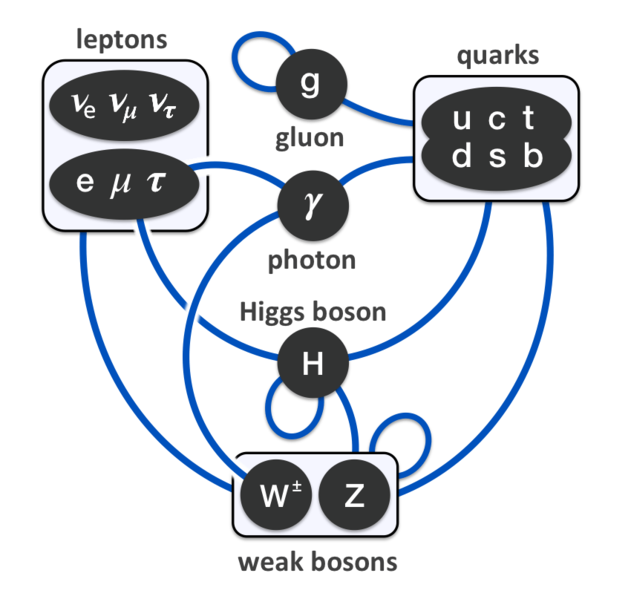
\includegraphics[width=0.9\textwidth]{SM_interactions.png}
    \caption{Schematic illustrating all the known particles in the SM and their interactions. Connections between different
    particles indicate that they interact. For the weak bosons ($W^{\pm}, Z$), gluons and the Higgs boson, self-interactions
    are also shown. Diagram is drawn by Eric Drexler.}
    \label{fig:sm_interactions}
\end{figure}

\clearpage
\section{Beyond the Standard Model: dark matter}

\graphicspath{{1_TheoreticalBackground/Figures/DM}}

Despite its triumphs, the SM fails to explain many astrophysical observations~\cite{Bertone:2004pz}.
One very important question that is closely related to this thesis is the existence of DM, which
refers to a form of matter that does not interact electromagnetically, and therefore neither emits or reflects light.
As will be explained within this section, strong evidence exists for the existence of DM, however the SM
does not have any explanation about this form of matter.
The first subsection below aims to give a brief overview of the evidence for the existence of DM.
The following subsection covers searches of DM in a wide variety of particle physics experiments.

\subsection{Experimental evidence for dark matter}
\label{subsec:dm_evidence}

Evidence for the existence of DM emerged from astrophysical observations within the 20th century. In 1933,
F. Zwicky~\cite{Zwicky:1933gu} observed that galaxies in the Coma cluster are moving faster than what
is expected, requiring a larger amount of gravitational force to keep them in their orbits. Since then, the
same phenomena has been observed within individual galaxies in the 1970s~\cite{Bertone:2004pz}. This can be observed
by looking at the rotation curves of the galaxies, namely the graph of circular velocities of stars and gas
as a function of distance from the galactic center. One such rotation curve, for the NGC 6503 galaxy, is shown in
Fig.~\ref{fig:galaxy_rot_curve}.

\begin{figure}[htbp]
    \centering
    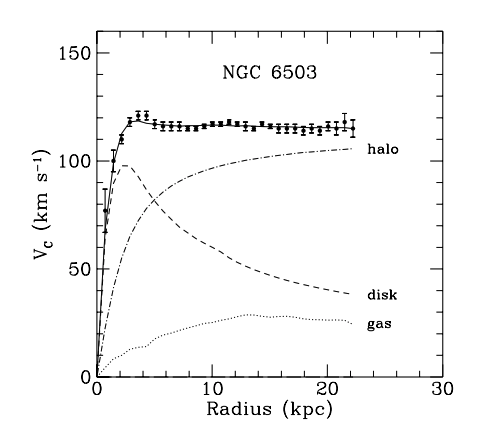
\includegraphics[width=0.7\textwidth]{galaxy_rot_curve.png}
    \caption{Rotation curve for the galaxy NGC 6503. The dashed and dotted lines represent the expected velocity profile
    from the disk (visible matter) and gas contributions, while the dash-dotted line represennts the halo (dark matter)
    contribution, required to explain the observed rotation curve. Taken from~\cite{Bertone:2004pz}.}
    \label{fig:galaxy_rot_curve}
\end{figure}

As can be observed from Fig.~\ref{fig:galaxy_rot_curve}, observed rotation curves usually exhibit a flat behavior at
large distances from the galaxy center. The contributions from the visible
disk and gas alone, however, cannot explain the observed rotation curves. 
From Newtonian dynamics, the expected circular velocity for a galactic object orbiting around a mass profile $M(r)$ 
can be written as

\begin{equation}
    v(r) = \sqrt{\frac{G M(r)}{r}}
\end{equation}
where $M(r) = 4\pi \int \rho(r') r'^{2} dr'$ and $\rho(r)$ is the mass density profile. Assumming visible matter, $v(r) \propto \frac{1}{\sqrt{r}}$,
hence the fact that the rotation curves are approximately flat implies the existence of DM with $M(r) \propto r$~\cite{Bertone:2004pz}.

Another piece of evidence for the existence of DM comes from the gravitational lensing effect~\cite{Mellier:1998pk}, which refers to the
phenomena where the trajectory of light bends in the vicinity of a massive object (``deflector''), due to the curvature in 
space-time near the deflector. The dependence of this bending on the mass density of the deflector implies that gravitational
lensing can probe the mass of deflectors, making it a unique tool to probe the DM distribution in gravitational systems. In other words,
the amount of deflector mass can be measured from the amount of deflection in the trajectory of light. The amount of bending can be
deduced by measuring the angular shift $\Delta\vec{\theta}$ of the source. The amount of lensing effect can also be extracted from
the distortion of the source. As an example, if the image source is a circular galaxy, to first approximation it can be shown that
the gravitational lensing effect transforms it into an ellipse~\cite{Mellier:1998pk}. Using the gravitational lensing technique, the
presence of large non-visible matter clusters was inferred, (see~\cite{1988ApJ...332...75N}).

Evidence on the existence of DM is also present on the galactic scale, coming from the precise measurements of the cosmic
microwave background (CMB) radiation~\cite{Hu:1995kot}. The CMB is the electromagnetic radiation originating from the propagation of photons
in the early Universe, when photons decoupled from baryons. Decades of experimental effort show that the CMB follows 
the spectrum of a blackbody radiation with $T=2.726$ K, and it is nearly isotropic,
with temperature fluctuations reaching only one part in $10^{5}$ of the mean~\cite{Bertone:2004pz}.
The residual anisotropies in the CMB can be studied to extract information about the abundance of baryons and matter in the Universe. 
This is achieved by fitting
a given cosmological model with a fixed number of parameters, $N$, and finding the best-fit parameters from the peak of $N$-dimensional
likelihood. Using the data from Wilkinson Microwave Anisotropy Probe (WMAP), one can obtain the following values for the baryonic matter
density $\Omega_{b} h^{2}$ and total matter density $\Omega_{H} h^{2}$~\cite{Bertone:2004pz}:

\begin{equation}
    \Omega_{b} h^{2} = 0.024 \pm 0.01 \quad \textrm{and} \quad \Omega_{M} h^{2} = 0.14 \pm 0.02
\end{equation}

where $h$ is Hubble's constant. Therefore, it can be inferred that the DM relic density is $\Omega_{DM} h^2 \approx 0.12$, indicating that
predictions based on WMAP data imply that DM is more abundant compared to baryonic matter by a factor of $\approx 6$. In summary, multiple
pieces of evidence, both at galactic and cosmological scales, suggest the existence of DM. 

\subsection{Searches for dark matter}

In an effort to explain the DM observations outlined in Sec.~\ref{subsec:dm_evidence},
multiple hypotheses have been proposed, where the DM is made out of particles that are not
described by the Standard Model (commonly called ``Beyond the Standard Model'', or ``BSM'' for short).
There are a wide range of models, where proposed types of particles include axions and weakly interacting 
massive particles (WIMPs)~\cite{Profumo:2017hqp}.

% In an effort to explain the DM observations outlined in Sec.~\ref{subsec:dm_evidence}, multiple hypotheses have been proposed. 
% Broadly speaking, one line of effort is to extend Newton's gravity and Einstein's general relativity~\cite{Famaey:2011kh}
% to try to explain discrepancies between the measured circular velocities of galactic objects and the corresponding observed mass. 

A WIMP refers to a new elementary particle which interacts via gravity\footnote{It is possible that WIMPs interact
with forces that are not described by the Standard Model, which is as weak as or weaker than the weak nuclear force.}.
Such particles are readily predicted by popular extensions of the Standard Model, including 
supersymmetry~\cite{Jungman:1995df}, models with extra dimensions~\cite{Dienes:1998vh}  
and little Higgs~\cite{Arkani-Hamed:2002ikv}. In the scenario where DM is made up of WIMPs, it is possible to
detect these new particles using a number of techniques in particle detectors. 

One such technique is direct detection, in which experiments look for signals from elastic scattering of DM
particles with ordinary matter. These experiments typically use detectors made out of liquid noble gases or crystals,
which are sensitive material which can generate detectable signals (such as scintillation light) in the event of a WIMP
passing through.
Such experiments include Xenon1T~\cite{XENON:2017vdw}, CRESST-II~\cite{Angloher:2011uu},
CDMSlite~\cite{SuperCDMS:2017nns}, LUX~\cite{LUX:2015abn} and PandaX-II~\cite{PandaX-II:2016vec}.
No evidence has been observed of DM particles through direct detection experiments, however, very stringent constraints
on the DM-nucleuon interaction cross section have been placed as a function of WIMP mass. 
As a notable example, XENON1T was able
to reach an upper bound of $\sigma_{\textrm{DM-nucleon}} < 7.7 \times 10^{47} \textrm{cm}^{-2}$ for a WIMP mass of 
$m_{\textrm{DM}} = 35$ GeV~\cite{XENON:2017vdw}.

Another technique for WIMP detection is indirect detection, in which experiments look 
for evidence of WIMP self-annihilation or decay products,
such as high-energy photons or neutrinos. These experiments look for secondary products coming from the WIMP
self-interactions, as opposed to attempting to directly observe signals from a WIMP itself. One such experiment is
Fermi-LAT~\cite{Fermi-LAT:2011vow}, which is a space-based instrument that detects gamma rays. It searches for an excess
of gamma ray emission that might indicate WIMP self-annihilation or decay. Another such experiment is IceCube~\cite{Iovine:2022aiw},
which is a neutrino observatory in the South Pole. IceCube can detect high-energy neutrinos produced by cosmic-ray interactions,
and observation of an excess of neutrinos can point to WIMP self-annihilation and decay processes. Similar to direct detection results,
no evidence of WIMPs has been observed to date, but stringent limits are placed in WIMP self-annihilation cross sections. 

Finally, another technique for WIMP searches is to produce them in particle detectors, such as the Large Hadron Collider 
(LHC)\footnote{See Sec.~\ref{sec:large_had_collider} for the description of the LHC.}. 
With a very large proton-proton collision
center of mass energy, $\sqrt{s} = 13$ TeV\footnote{The center of mass energy for the pp collision data (2016-2018) 
used in the analysis described in this thesis is $\sqrt{s} = 13$ TeV. 
However, it should be noted that starting from 2022 data-taking, this center of mass
energy has been increased further to $\sqrt{s} = 13.6$ TeV.}, many WIMP models predict that pair production of WIMPs would be
within the kinematic reach, provided that there is some interaction between the SM sector and WIMPs. Hence, at particle colliders,
one can expect to observe the process $\textrm{pp} \rightarrow \chi \bar{\chi} + X$, where $\chi$ refers to the WIMP (and $\bar{\chi}$
its antiparticle), and $X$ is a placeholder for other physics objects in the final state, depending on the model being considered.

One interesting class of models that is relevant to the analysis described in this thesis is the so called Higgs portal models~\cite{Argyropoulos:2021sav}.
Such models hypothesize that there are beyond SM interactions of the Higgs boson with the WIMPs (commonly also called the ``dark sector''),
and proton-proton colliders are excellent machines to probe such interactions of the Higgs boson through its decay products, \textit{i.e.} 
$\textrm{H} \rightarrow \chi \bar{\chi}$, because of the large rates of Higgs bosons being produced. These models are discussed in more detail in the
following section, where Sec.~\ref{subsec:higgs_portal_theory} gives an overview of the theory, and Sec.~\ref{subsec:exp_signatures} gives an overview
of the experimental signatures expected in proton-proton collisions.  





\section{Higgs portal models}

\graphicspath{{1_TheoreticalBackground/Figures/HiggsPortal}}

The discovery of the Standard Model (SM) Higgs boson by ATLAS and CMS experiments~\cite{Nisati:2015iwc} has paved the way for a new direction
in the searches for DM, in which one can explore the potential connections between the Higgs boson and the dark sector.
Dark sector refers to a Beyond the Standard Model (BSM) sector that contains the dark matter (DM) particle, and is almost decoupled from 
the SM. An interesting possibility is that the Higgs boson acting as a portal between the SM and dark sectors through
couplings to both sectors. There are both experimental and theoretical arguments that make this an interesting possibility.
Experimentally, the Higgs sector is far less explored and constrained, compared to the other sectors of the SM. Theoretically,
Higgs field is the only field that allows to write down a renormalizable
coupling to the dark sector, if DM is uncharged under the SM gauge group~\cite{Argyropoulos:2021sav}. Therefore, introducing 
DM-Higgs boson couplings is a well-motivated extension of the SM. Provided that the DM particles are not very heavy,
i.e. $m_{DM} < \frac{m_H}{2}$, such couplings would allow the Higgs boson to decay into DM particle
pairs, $\chi \bar{\chi}$. An example of this process is shown in Fig.~\ref{fig:vbfhinv_signal_diag}, where the SM Higgs boson
is produced via the Vector Boson Fusion (VBF) process, and decays into $\chi\bar{\chi}$ final state.

\begin{figure}[htbp]
    \centering
    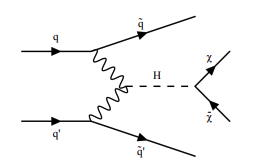
\includegraphics[width=0.4\textwidth]{vbf_signal_diagram.png}
    \caption{VBF production of a SM-like Higgs boson, where Higgs boson decays into a pair of DM particles, $\chi\bar{\chi}$,
    in the context of Higgs portal models. Diagram is taken from~\cite{VBFHinvAnalysisPaper}.}.
    \label{fig:vbfhinv_signal_diag}
\end{figure}

Given that the nature of the dark sector is mostly unknown, there are a multiple number of scenarios for the $H \chi \bar{\chi}$ coupling,
where the DM particle $\chi$ can be a scalar, a vector or a Majorana fermion~\cite{Djouadi:2011aa}. A brief overview of the 
theory of Higgs portal models under these different scenarios is provided in Sec.~\ref{subsec:higgs_portal_theory}, and the experimental
implications in particle colliders are discussed in Sec.~\ref{subsec:exp_signatures}.

\subsection{Theory}
\label{subsec:higgs_portal_theory}

This subsection aims to give a brief overview of the Higgs portal theories for different scenarios, following the footsteps of~\cite{Djouadi:2011aa}.
For the scenarios under which the DM particle is a scalar, vector or a Majorana fermion the corresponding Lagrangian terms are 

\begin{equation}
    \begin{split}
        \mathcal{L}_{S} &= -\frac{1}{2} m_{S}^{2} S^{2} - \frac{1}{4} \lambda_{S} S^{4} - \frac{1}{4} \lambda_{HSS} H^{\dag} H S^{2} \\
        \mathcal{L}_{V} &= -\frac{1}{2} m_{V}^{2} V_{\mu} V^{\mu} - \frac{1}{4} \lambda_{V} (V_{\mu} V^{\mu})^{2} + \frac{1}{4} \lambda_{HVV} H^{\dag} H V_{\mu} V^{\mu} \\
        \mathcal{L}_{f} &= -\frac{1}{2} m_{f} \bar{\chi} \chi - \frac{1}{4} \frac{\lambda_{Hff}}{\Lambda} H^{\dag} H \bar{\chi} \chi
    \end{split}
    \label{eq:higgs_portal_lagrangians}
\end{equation}

where the last terms represent the coupling between the DM-particle and SM-like Higgs boson, with $\lambda_{H\chi\bar{\chi}}$ being the coupling constants for each case.
It should be noted that the $H\chi\bar{\chi}$ coupling is not renormalizable in the fermionic case. The $S^{4}$ and $(V_{\mu} V^{\mu})^{2}$ are self-interaction terms
for scalar and vector DM particles, respectively. The first terms in each Lagrangian correspond to the mass term for the DM particle.

After electroweak symmetry breaking, the doublet field $H$ is written as $\phi(x) = \frac{1}{\sqrt{2}} \begin{pmatrix} 0, & v + h(x) \end{pmatrix}$ with $v = 246$ GeV
being the vacuum expectation value of the Higgs field. In that case, the physical masses of the DM particles can be written as~\cite{Djouadi:2011aa}

\begin{equation}
    \begin{split}
        M_{S}^2 &= m_{S}^2 + \frac{1}{2} \lambda_{hSS} v^{2} \\
        M_{V}^2 &= m_{V}^2 + \frac{1}{2} \lambda_{hVV} v^{2} \\
        M_{f}   &= m_{f}   + \frac{1}{2} \frac{\lambda_{hff}}{\Lambda} v^{2}
    \end{split}
\end{equation}

Provided that the DM particle $\chi$ is light enough for the $H \rightarrow \chi \bar{\chi}$ decay to occur (i.e. $M_{\chi} < M_{H} / 2$), there will be a non-zero
branching fraction for this decay of the Higgs boson, i.e. $B(H \rightarrow \chi \bar{\chi}) = \frac{\Gamma_{\chi\bar{\chi}}}{\Gamma_{H}} \neq 0$. The decay width for
$H \rightarrow \chi \bar{\chi}$ can be written as follows for the different scenarios being considered~\cite{Djouadi:2011aa}

\begin{equation}
    \begin{split}
        \Gamma_{h \rightarrow SS} &= \frac{\lambda_{hSS}^{2} v^{2} \beta_{S}}{64 \pi m_{H}} \\
        \Gamma_{h \rightarrow VV} &= \frac{\lambda_{hVV}^{2} v^{2} m_{h}^{3} \beta_{V}}{256 \pi M_{V}^{4}} \left( 1 - 4 \frac{M_V^2}{m_h^2} + 12 \frac{M_V^4}{m_h^4} \right) \\
        \Gamma_{h \rightarrow ff} &= \frac{\lambda_{hff}^{2} v^{2} m_{h} \beta_{f}^{3}}{32 \pi \Lambda^{2}}
    \end{split}
\end{equation}

where $\beta_{X} = 1 - \sqrt{1 - 4 M_X^2 / m_h^2}$. 
Therefore, observing these decays predicted by the Higgs portal models in particle colliders would be an important
leap towards understanding BSM physics. Observing these decays in particle colliders is the topic of the next subsection.

\subsection{Experimental signatures in colliders}
\label{subsec:exp_signatures}

Under the assumption of the DM particle ($\chi$) being a WIMP candidate, it is assumed that $\chi$ does not have electromagnetic interactions. That would imply
that in particle detectors like ATLAS and CMS, these particles would pass through without interacting with the detector components. Therefore, the event of a
$H \rightarrow \chi \bar{\chi}$ decay can be inferred by a large amount of transverse momentum imbalance in the event, i.e. large $p_T^{miss}$ (provided that there
is visible energy coming from other final state particles). Because of this, such decays are often referred to as ``invisible decays of the Higgs boson'', and very
commonly denoted as $\hinv$ This thesis will follow the same notation.

Such decays can be probed using proton-proton collisions by targeting events with the main production modes of the Higgs boson. Feynman diagrams for these production 
modes are shown in Fig.~\ref{fig:all_higgs_prod}. A very nice overview of all the production modes, 
together with their cross sections and kinematics are given in~\cite{Djouadi:2005gi}.

\begin{figure}
    \centering
    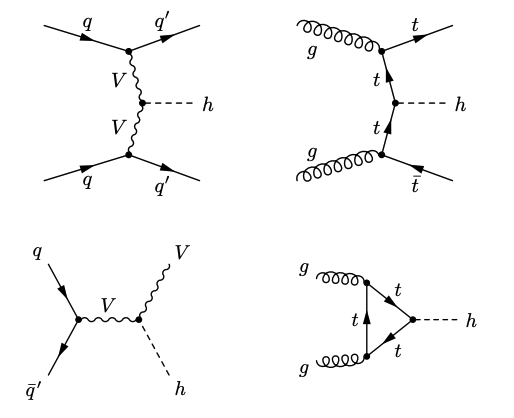
\includegraphics[width=0.7\textwidth]{all_higgs_prod.png}    
    \caption{Main production modes of the Higgs boson at a proton-proton collider. The production modes are vector boson fusion (top left), production in association with
    a pair of top quarks (top right), in association with a vector boson (bottom left), and via gluon-gluon fusion (bottom right). Diagrams are taken from~\cite{Argyropoulos:2021sav}.}
    \label{fig:all_higgs_prod}
\end{figure}

At the Large Hadron Collider (LHC), with a proton-proton collision center of mass energy of $\sqrt{s} = 13$ TeV, the dominating production mode is the gluon-gluon fusion. Events from 
this production mode can be probed by targeting final states with an energetic hadronic jet\footnote{Hadronic jets arise from the hadronization of the
underlying final state quarks. Since individual quarks carry color charge, they cannot be observed individually due to the hypothesis of color confinement,
which arises from the gluon-gluon self interactions. On a mathematical basis, this is explained by the $g_{S} f^{ijk} G_{\mu}^{j} G_{\nu}^{k}$ terms appearing in 
Eq.~\ref{eq:gluon_field_strength}, which arise due to the non-commuting nature of SU(3) generators. Hence, jets are the corresponding 
experimental observables in particle colliders.} 
coming from initial state radiation, together with large $p_T^{miss}$ due to the invisible decay
of the Higgs boson. This is the so called ``monojet'' search, while there was no evidence observed for such events, this channel provided important constraints on the invisible
branching ratio of the Higgs boson, $B(\hinv) < 27.8\%$~\cite{CMS:2021far}. The associated production with a vector boson or a top-antitop quark pair have smaller cross sections,
but still are important final states to probe Higgs portal models, see for example~\cite{CMS:2023sdw}.

Search for $\hinv$ decays through the remaining production mode, vector boson fusion (VBF), is the topic of this thesis.
VBF has a lower production cross section, which is roughly an order of magnitude lower than the gluon-gluon fusion at $\sqrt{s} = 13$ TeV. But, it is still
a very sensitive channel in the searches of new physics. This is due to the uniqueness of the experimental signature of the final state, which comprises of two energetic jets with large
spatial separation in the detector, and a large $p_T^{miss}$ because of the invisible decay of the Higgs. These two jets typically have small scattering angles with respect to the proton-proton
collision axis\footnote{A detailed explanation for this can be found in~\cite{Djouadi:2005gi}. It can be shown that the matrix element $\mathcal{M}$ is bounded by $1 / (p_T^2 + M_V^2)$,
where $p_T$ is the transverse momentum of the outgoing quarks, and $M_V$ is the mass of the vector boson. Hence, while the final state quarks are relatively energetic, the VBF cross-section is
suppressed for $p_{T} \gg M_{V}$, making the quarks (and hence the resulting final state jets from hadronization) more forward.}, 
hence making them more forward in the detector and well-separated from each other. This unique final state signature of the VBF process can be used to reject a large amount of
SM backgrounds, hence making this channel very sensitive to signal. In fact, the previous $\hinv$ searches done by collider experiments showed that VBF is the most sensitive channel, resulting
in the tightest constraints put on the $\brhinv$, see for example~\cite{CMS:2018yfx}. Hence, it is experimentally very motivating to continue the VBF $\hinv$ search with the new data coming in from
the Large Hadron Collider (LHC).

The rest of this thesis is structured as follows. Chapter~\ref{chap:apparatus} will give an overview of the experimental apparatus used to search for VBF $\hinv$ decays, namely the Large
Hadron Collider (LHC) and the Compact Muon Solenoid (CMS) detector. Chapter~\ref{chap:data_analysis} will then describe the analysis strategy, highlighting the analysis selections, the maximum
likelihood fit procedure and systematic uncertainties considered in the analysis. Chapter~\ref{chapter:results} will describe the results of the analysis and it's physics interpretations. Finally,
Chapter~\ref{chapter:outlook} will give perspective on the future direction of the CMS detector and the VBF $\hinv$ analysis, outlining upgrades on the detector and the triggering system, and
the search for new analysis methodologies using novel machine learning techniques.
\cleardoublepage

% -------------------------------------
% CHAPTER 2: THE BODY OF THESIS
% -------------------------------------
\chapter{Experimental Apparatus}
\label{chap:apparatus}

\graphicspath{{2_Experimental_Apparatus/Figures/}}

\section{The Large Hadron Collider}
\label{sec:large_had_collider}

The Large Hadron Collider (LHC), located near Geneva, Switzerland, is a circular particle accelerator, 
consisting of a 27-kilometer ring of superconducting magnets.
Two sets of proton bunches travel along the circular tunnel in opposite directions,
then collide at the experiment sites. The four large experiments located at the LHC ring are CMS, ATLAS, LHCb, and ALICE. The CMS and ATLAS
detectors are multi-purpose, while LHCb focuses on b-quark physics, and ALICE focuses on heavy-ion physics. The center-of-mass energy 
for the proton-proton collision for Run 2 is 13 TeV.

Protons are accelerated through a chain of accelerators before they reach LHC, which is shown in Fig.~\ref{fig:lhc_diagram}.
Each machine boosts the energy of protons before injecting it into the next machine in the sequence. Linear Accelerator 4 (LINAC4)
is the source of protons, accelerating $\textrm{H}^{-}$ ions to 160 MeV to prepare them to enter the Proton Synchotron Booster (PSB). During the injection
to PSB, the electrons are stripped, leaving only the protons. These protons are accelerated to 2 GeV for injection to Proton 
Synchotron (PS), which increases the beam energy to 26 GeV. The proton beams are then sent to Super Proton Synchotron (SPS), where they are accelerated
to an energy of 450 GeV. Finally, the proton beams are transferred to the two beam pipes of the LHC, where it takes 20 minutes for the protons to reach
their maximum energy of 6.5 TeV. 

\begin{figure}[htb]
    \begin{minipage}[t]{\linewidth}\centering
        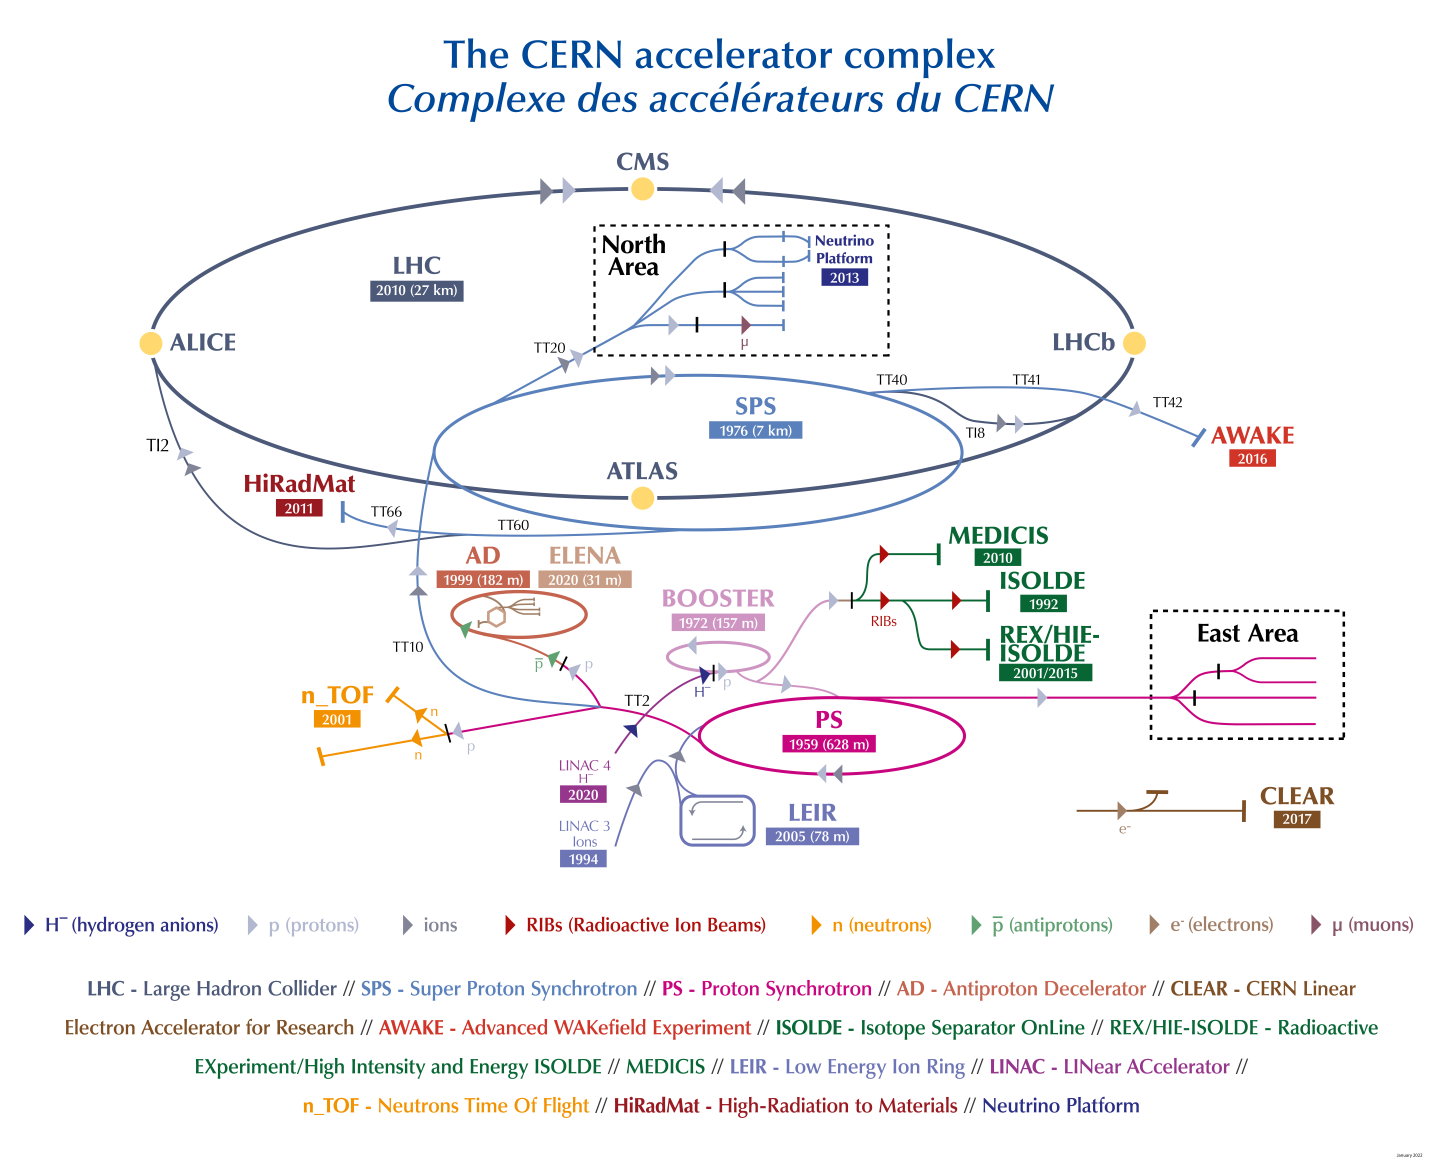
\includegraphics[width=15cm]{lhc_complex.png}
    \end{minipage}
    \caption{Diagram of the CERN accelerator complex, showing the LHC and the chain of other accelerator rings. 
    Each ring boosts the energy of accelerated particles before injecting it into the next ring in the sequence.
    The diagram is taken from \cite{LHCAcceleratorComplex}.}
    \label{fig:lhc_diagram}
\end{figure}

The LHC had a successful Run 1 between 2010 and 2013, where the center-of-mass energy for proton-proton collisions was 8 TeV. This first run was marked 
by the discovery of the Higgs boson by ATLAS and CMS experiments in 2012. After a long shutdown, the center-of-mass energy was increased to 13 TeV, and the LHC
operated from 2016 to 2018 for Run 2 data taking. During Run 2, the instantenous luminosity was about $1 \times 10^{34} \ \lumiunit$, corresponding to around 
25 proton-proton collisions per bunch crossing. The integrated luminosity corresponding to Run 2 data taken by the CMS experiment is measured to be 137 $\fbinv$, 
with 1.6\% overall uncertainty \cite{lumi:2018,lumi:2017,lumi:2016}.

\section{The CMS detector}

The CMS detector is a multi-purpose detector, designed trigger on \cite{cms:l1_paper,cms:hlt_paper} and detect muons, electrons, photons, charged and 
neutral hadrons \cite{cms:elepho_paper,cms:muon_paper,cms:vertex_paper}. To be able to identify this wide range of particles, the CMS detector uses a combination of signals from different sub-detectors. These signals
are then used in the Particle-Flow (PF) algorithm to reconstruct the particles in the event. The sub-detectors in the CMS detector are:

\begin{itemize}
    \item Tracking system
    \item Electromagnetic calorimeter (ECAL)
    \item Hadron calorimeter (HCAL)
    \item Muon system
\end{itemize}

CMS detector also uses a two-level trigger system \cite{cms:l1_paper,cms:hlt_paper}, to make physics-based decisions on the data being saved to disk, 
therefore reducing the output rate. In the following sub-sections, the functionality of these subsystems and the overall design of the CMS detector are discussed.

\subsection{Overall layout}

The CMS detector has an overall length of 28.7 m, and weighs 14000 tonnes. The cylindrical detector
has a diameter of 15 m, as shown in Fig.~\ref{fig:cms_overall_diagram}. The CMS detector has a superconducting solenoid,
which has an internal diameter of 7 m, and creates a magnetic field of 3.8 T. This magnetic field bends the charged particles
as they pass through the detector, enabling the measurement of their momentum from the curvature of their tracks.


\begin{figure}
    \begin{minipage}[t]{\linewidth}\centering
        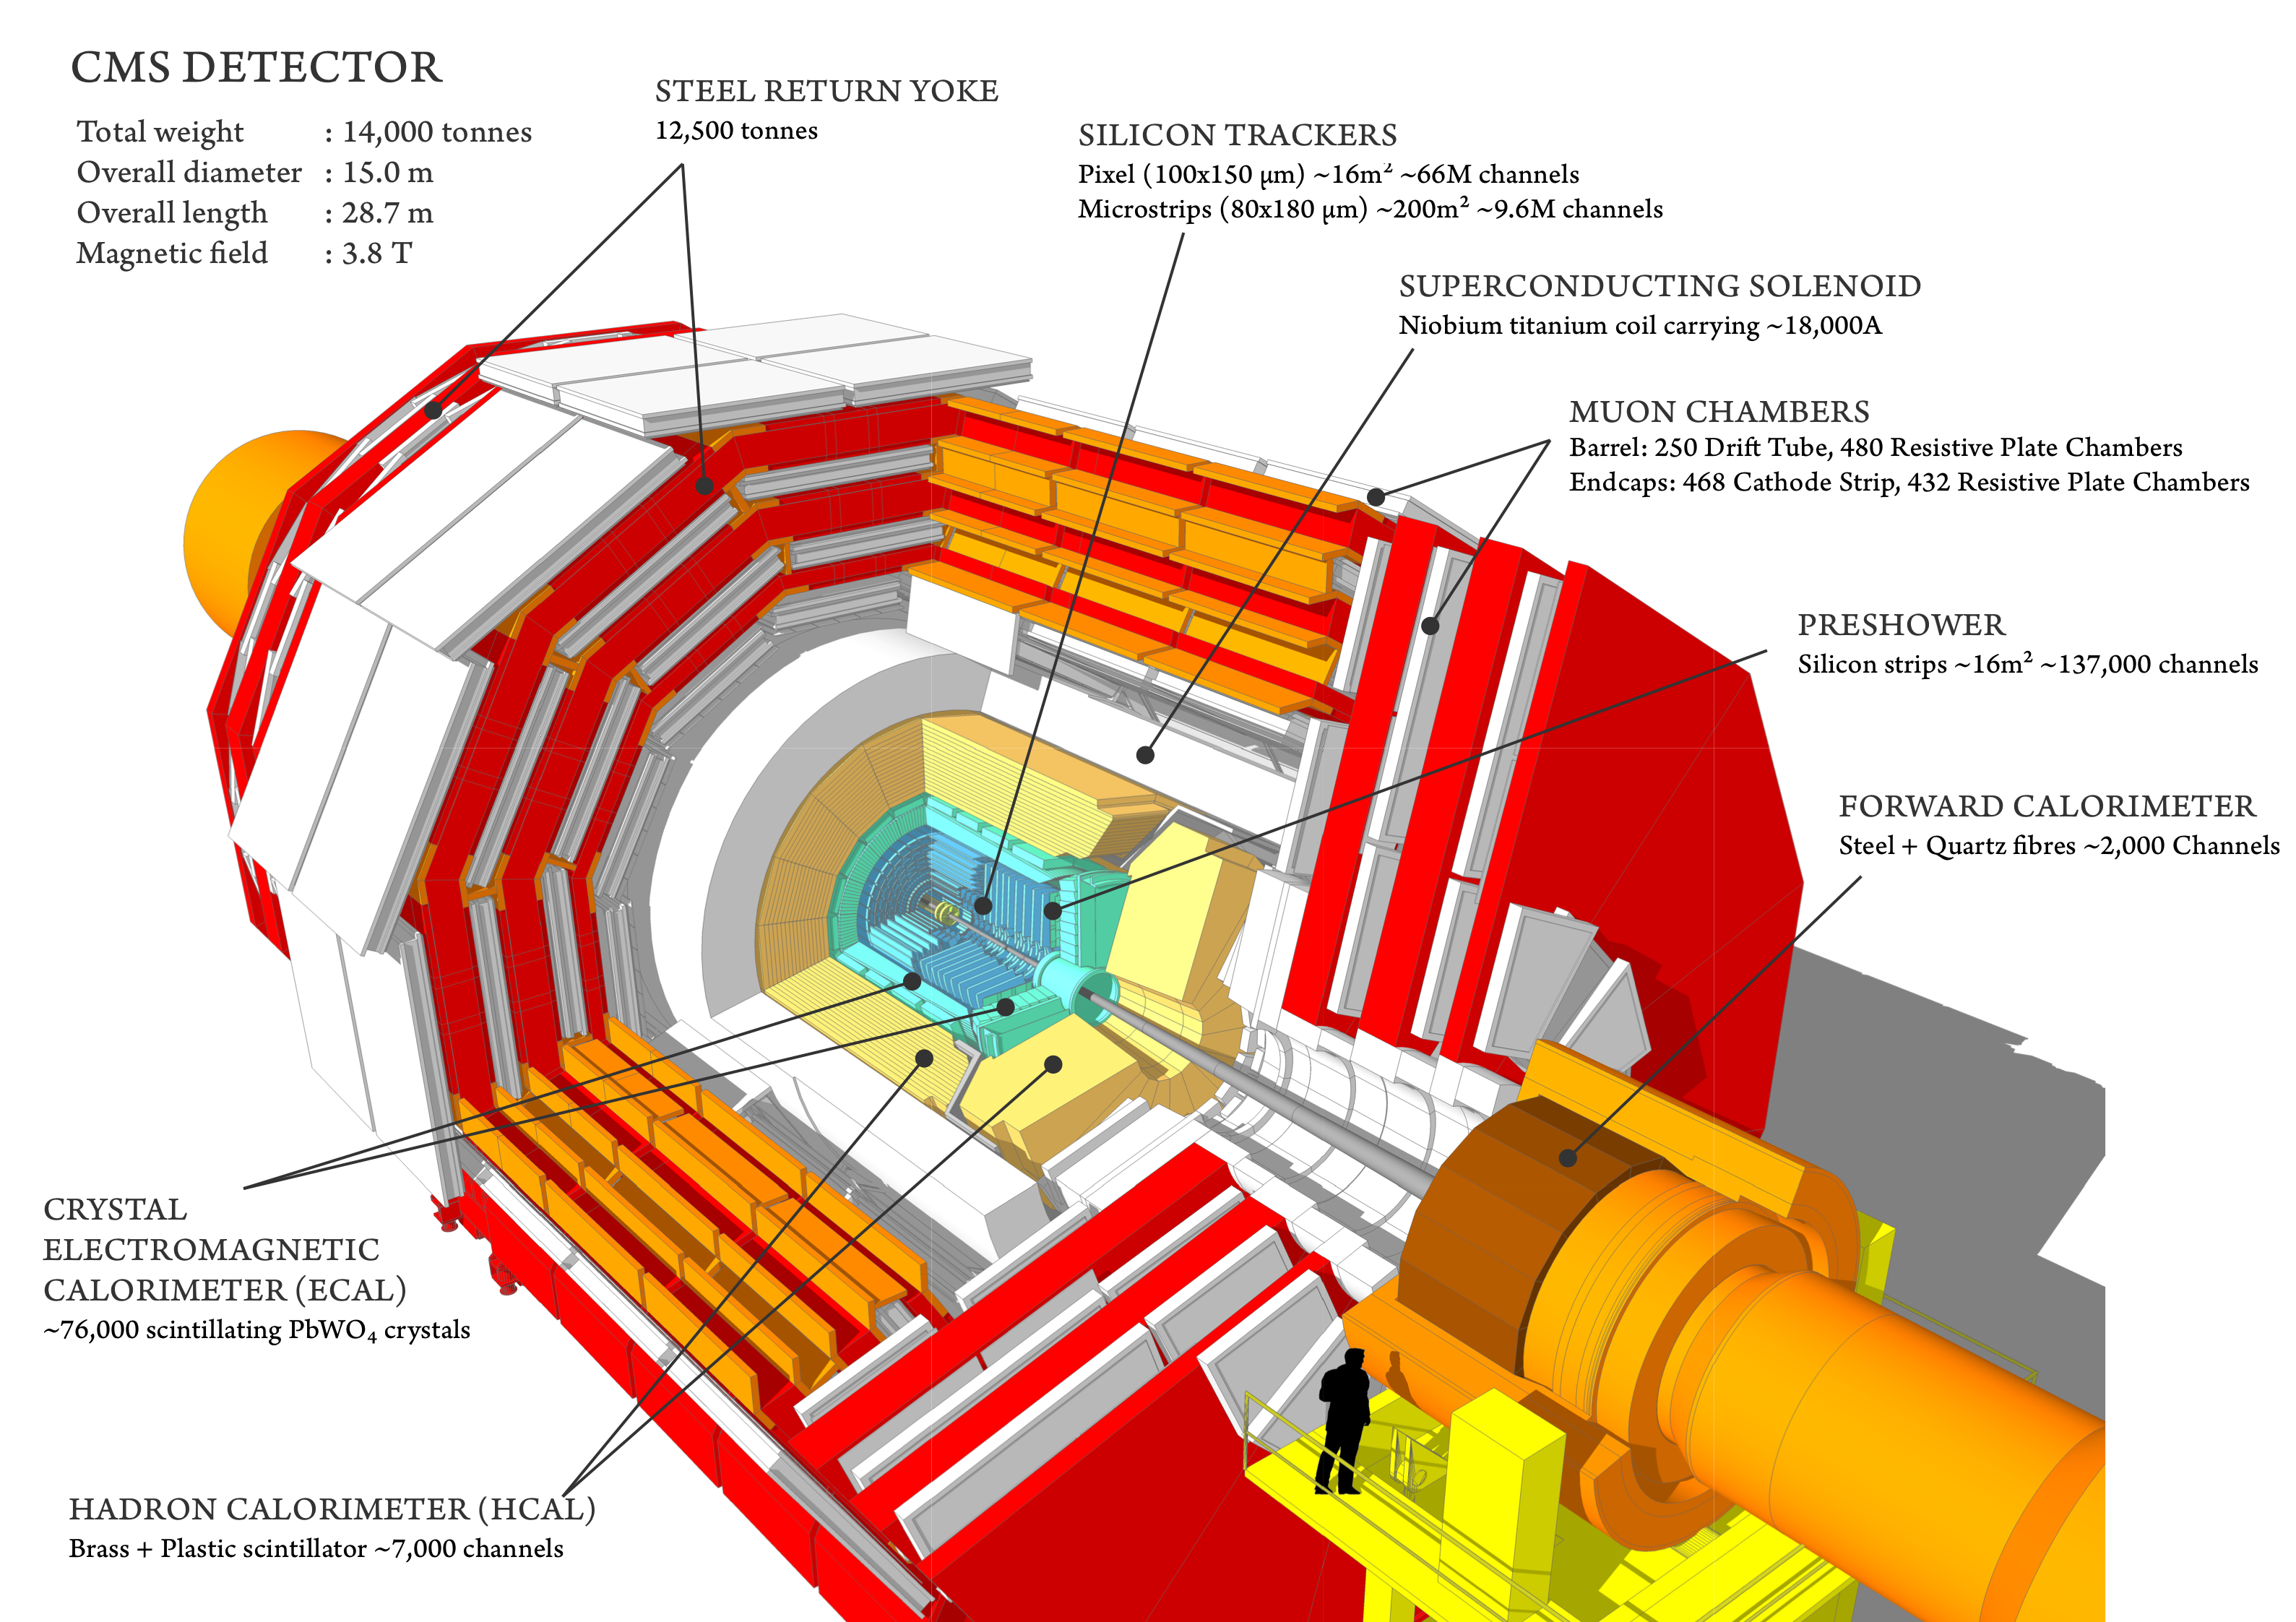
\includegraphics[width=15cm]{cms_detector.png}
    \end{minipage}
    \caption{Sectional view of the CMS detector. The LHC beams travel in opposite directions 
    along the central axis of the CMS cylinder colliding in the middle of the CMS detector \cite{detector:cms_overall}.}
    \label{fig:cms_overall_diagram}
\end{figure}

Within the solenoid volume are a silicon pixel and strip tracker, a lead tungstate crystal electromagnetic calorimeter (ECAL), 
and a brass and scintillator hadron calorimeter (HCAL), each composed of a barrel and two endcap sections. Forward calorimeters
are installed in the high psuedo-rapidity range to extend the coverage of the detector. Outside of the solenoid volume,
a muon detection system is installed, where muons are measured in gas-ionization detectors embedded in the steel flux-return yoke.

In the CMS detector, a right-handed coordinate system is used. The x-axis points to the center of the LHC ring, the y-axis points up, 
and the z-axis point along the beam in the counter-clockwise direction. Due to the cylindrical symmetry of the detector geometry, the angular
coordinates of $\eta$ and $\phi$ are often used to describe event kinematics. $\phi$ is the azimuthal angle, defined to be 0 along the x-axis,
and $\frac{\pi}{2}$ along the y-axis. $\eta$ is the psuedorapidity, which depends on the angle from the z-axis, $\theta$, with the following
equation: $\eta = -\ln[{\tan({\frac{\theta}{2}})}]$. This way, $\eta$ equals to 0 along the z-axis, directly perpendicular to the beam-axis,
and $|\eta| \rightarrow \infty$ as the $\theta \rightarrow \frac{\pi}{2}$, $\textit{i.e.,}$ perpendicular to the beam axis. Most detector coverage
extends to $|\eta| \approxeq 5$. 

\subsection{Tracking system}

The innermost layer of the CMS detector is the tracking system. This tracking system consists of a silicon pixel detector and a silicon strip detector, 
referred to as the inner tracker and the outer tracker, respectively. Both are used to reconstruct tracks of charged particles, under the influence of
the 3.8 T magnetic field generated by the solenoid. The inner pixel detector has higher granularity, therefore it can reconstruct tracks more accurately near
the beam pipe, where the track density is higher.

Tracks of charged particles are crucial objects for CMS, because they allow measurement of the momenta and electrical charge of particles. These particles include
electrons, muons, taus and charged hadrons. The identification of tracks also allow the reconstruction of the proton-proton collision vertices in the event. This enables
the identification of the primary vertex in the event with the highest sum of $p_{\textrm{T,track}}^{2}$. Thus, the rest of the vertices can be identified as pile-up (PU),
and charged particles from these PU vertices can be rejected in object reconstruction. Track reconstruction also allows identification of b-quarks using displaced
vertices. 

The CMS inner tracker was upgraded during the year-end technical stop of the LHC in 2016/2017, referred to as the Phase-1 upgrade \cite{cms:tracker_upgrade},
in order to handle the instantaneous luminosity that exceeds the previously designed maximum value of $1 \times 10^{34} \ \lumiunit$. Utilizing a new 
beam pipe with smaller radius installed during the LHC Long Shutdown 1 (LS1), the Phase-1 pixel detector sits closer to the beam center, with 4 barrel layers 
(L1-L4) at radii of 29, 68, 109, and 160 mm, compared to the original three layers at 44, 73, and 102 mm. There is also an additional endcap disk on each end 
closer to the collision point. Therefore, there are now three disks at each end with distances of 291, 396, and 516 mm from the center of the detector, compared 
to the original three layers at 345 and 465 mm. This new layout is optimized to have 4-hit coverage for tracks within $|\eta| < 2.5$. The original and the upgraded
pixel detector layouts are shown in Fig.~\ref{fig:cms_tracker_upgrade}.

\begin{figure}
    \begin{minipage}[t]{\linewidth}\centering
        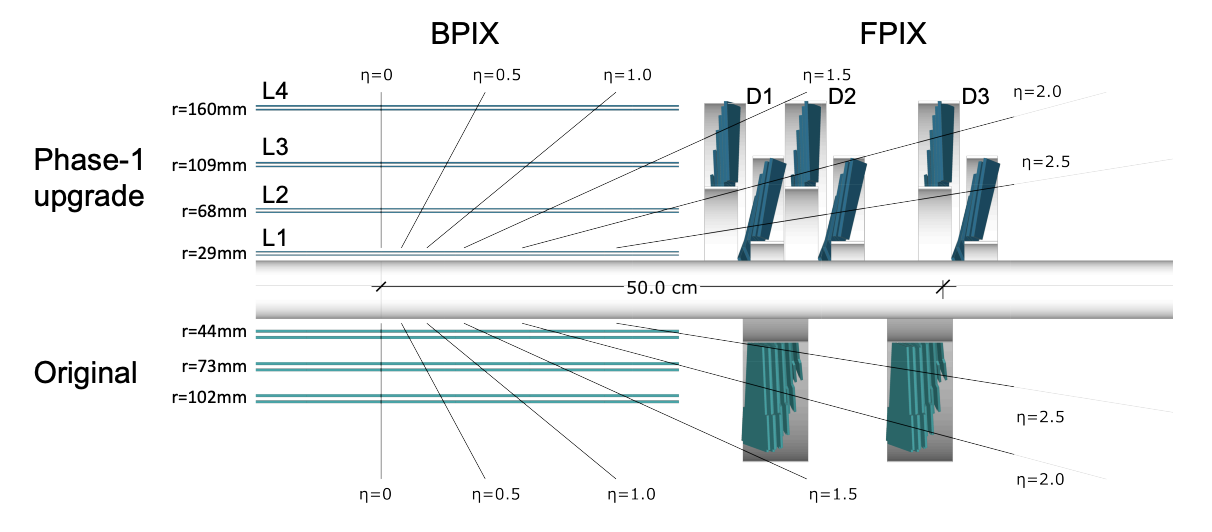
\includegraphics[width=15cm]{inner_tracker_layout.png}
    \end{minipage}
    \caption{Comparison of the layouts between the original pixel detector (bottom) and the Phase-1 upgraded pixel detector (top) \cite{cms:tracker_upgrade}.}
    \label{fig:cms_tracker_upgrade}
\end{figure}

Outside of the pixel detector, the silicon strip tracker is installed, which consists of three subsystems:  the Tracker Inner Barrel and Disks (TIB/TID), 
the Tracker Outer Barrel (TOB), and the the Tracker EndCaps (TEC). Their radii range from 20 cm to 116 cm and are up to 282 cm away from the detector center 
in the z direction. The layout of the silicon strip tracker, together with the 2016 version of the pixel detector, is shown in Fig.~\ref{fig:cms_full_tracker_layout}.

\begin{figure}
    \begin{minipage}[t]{\linewidth}\centering
        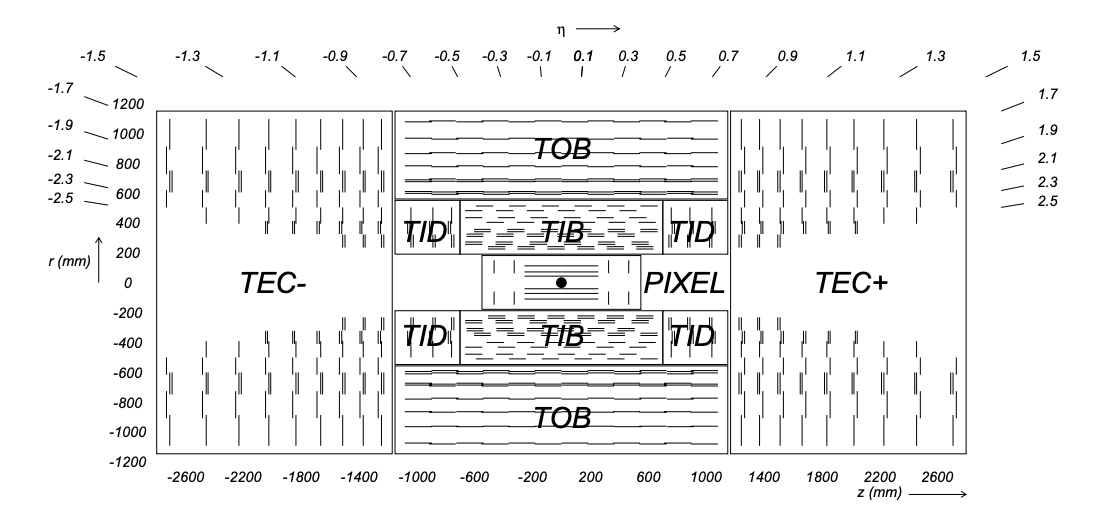
\includegraphics[width=15cm]{full_tracker_layout.png}
    \end{minipage}
    \caption{Schematic cross section through the CMS tracker. Notice that the pixel detector is shown as the 2016 version.
    The image is taken from \cite{cms:cms_experiment}.}
    \label{fig:cms_full_tracker_layout}
\end{figure}

\subsection{Electromagnetic calorimeter}

The electromagnetic calorimeter (ECAL) is installed as the second layer of the detector, outside the inner and outer tracking systems. It is made of
61200 lead tungstate ($\textrm{PbWO}_{4}$) crystals mounted in the barrel (EB), and 7324 of those crystals in each of the 2 endcaps (EE). 
The $\textrm{PbWO}_{4}$ crystals make
a radiation-resistent high-granularity calorimeter, due to it's high density and short radiation length. The EB section covers a psuedorapidity range
$|\eta| < 1.479$, and the two EE sections cover $1.479 < |\eta| < 3.0$.

The energy of particles, primarily electrons and photons, are measured through the scintillation effect. Photons emitted from the scintillation are 
collected by the avalanche photodiodes (APD) in the barrel and vacuum phototriodes (VPT) in the EE. Two preshower detectors are placed on the inner side
of the EEs, which helps to distinguish high-energy photons from pions, which can decay into a pair of closeby photons. The preshower is a sampling 
calorimeter made of two planes on each end. Each plane has a layer of lead radiators to produce electromagnetic showers from incoming photons and electrons, 
and a silicon strip detector to mea- sure the energy and shower profile. The silicon strips are placed with a width of 2 mm, and are oriented in perpendicular 
directions between two layers, giving a much finer granularity than EE and EB. 

The crystals in the barrel section are contained by 1 mm wall of aluminum, which constitues a submodule. Submodules are assembled into a module, 
and every four of each constitute a supermodule. The crystals in the EE are organized in units of identically shaped $5 \times 5$ crystals called supercrystals. 
Each EE is divided into two halves. The structure of the ECAL is shown in Fig.~\ref{fig:ecal_layout}.

\begin{figure}
    \begin{minipage}[t]{\linewidth}\centering
        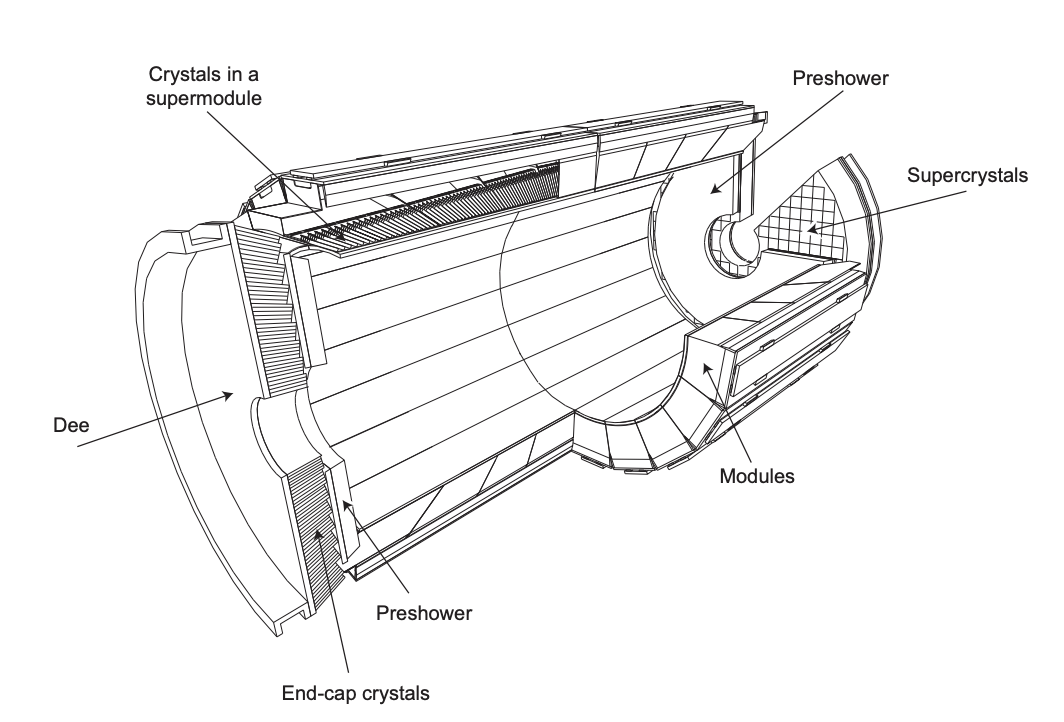
\includegraphics[width=15cm]{ecal_layout.png}
    \end{minipage}
    \caption{Layout of the CMS electromagnetic calorimeter showing the arrangement of crystal
    modules, supermodules and endcaps, with the preshower in front \cite{cms:cms_experiment}.}
    \label{fig:ecal_layout}
\end{figure}


\subsection{Hadron calorimeter}
\label{subsec:hcal}

The hadron calorimeter (HCAL) is designed to measure the energy of hadrons, which is specifically important for reconstructing and measuring the energy of
hadron jets. The HCAL is composed of several parts: 

\begin{itemize}
    \item A barrel part (HB), which sits between the ECAL and the magnet coil, covering $|\eta| < 1.3$. 
    \item An endcap part (HE), covering $1.3 < |\eta|< 3$.
    \item Forward hadron calorimeters (HF), which are placed close to the beam pipe to capture outgoing particles with small angles, covering up to $|\eta| < 5$.
\end{itemize}

Due to the limited space between the ECAL and the magnet coils, additional hadron calorimeters (HO) are placed outside of the magnet coils to help 
contain hadron showers. The layout of the HCAL detector is shown in Fig.~\ref{fig:hcal_layout}.

The majority of HCAL is a sampling calorimeter made of alternating absorbing layers of brass and plastic scintillating layers. 
The forward calorimeter HF utilizes a different design, which consists of a steel absorber and quartz fibers that generate Cherenkov light, 
in order to operate in a much harsher radiation environment, compared to other parts of the calorimeter.

\begin{figure}
    \begin{minipage}[t]{\linewidth}\centering
        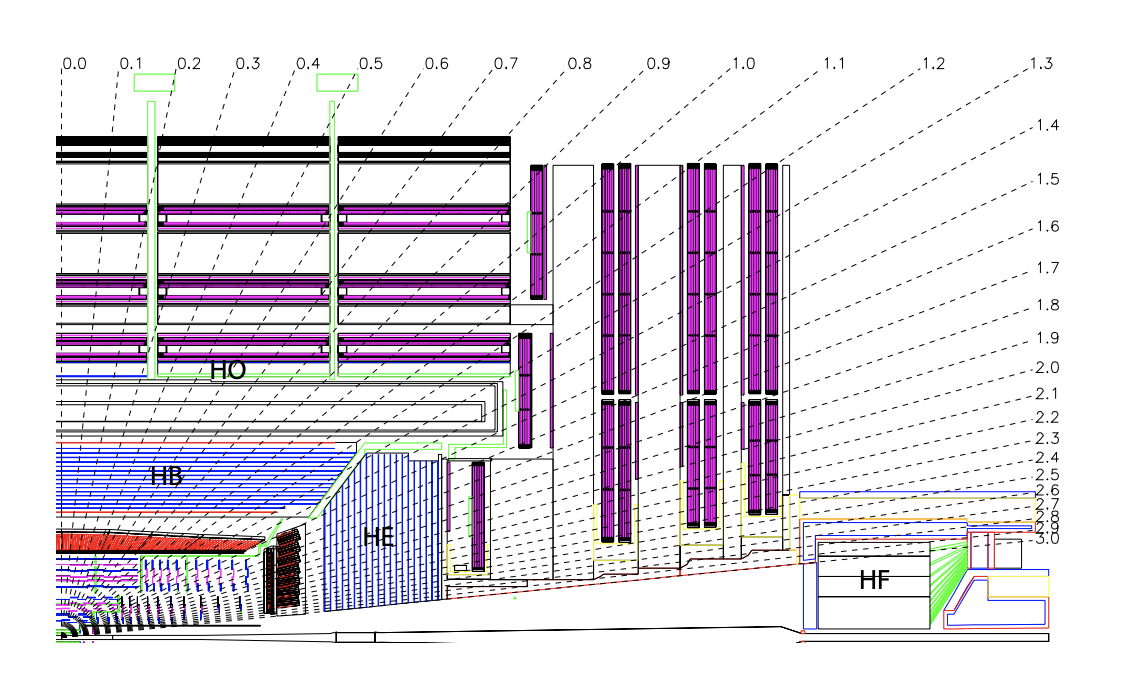
\includegraphics[width=15cm]{hcal_layout.png}
    \end{minipage}
    \caption{Longitudinal view of the CMS detector showing the locations of the hadron barrel (HB), endcap (HE), outer (HO) 
    and forward (HF) calorimeters ~\cite{cms:cms_experiment}.}
    \label{fig:hcal_layout}
\end{figure}

\subsection{Muon system}

Muon detection is of great importance to the CMS, since it is a powerful tool for recognizing signatures of interesting physics processes. Muons also have the
potential to be reconstructed with a larger resolution since they are not affected by radiative losses in the tracker material, compared to electrons. 

The muon system is installed in the psuedo-rapidity range of $|\eta| < 2.4$, consisting of drift tubes (DTs), cathode strip chambers (CSCs) and 
resistive plate chambers (RPCs). The DTs are placed in the barrel and cover $|\eta| < 1.2$, where the particle rate and the 
magnetic field are low. The CSCs, due to their fast response time, fine segmentation, and radiation resistance, are used in the endcap, covering
$0.9 < |\eta| < 2.4$. The RPCs are inserted into both barrel and endcaps to provide redundant trigger system with a time resolution of 1 ns, 
which is much shorter than the bunch crossing interval of 25 ns.

\subsection{Trigger system}
\label{subsec:trigger_system}

With a proton-proton bunch crossing interval of $25$ ns, collecting and saving all collision events at a rate of $400$ MHz in unsustainable, 
due to limitations in both storage space and data transfer rates. 
Storing all the events at this rate is also unnecessary, since interesting events with high-energy physics objects occur at a much
lower rate.

To select the events of interest and reduce the rate of data being saved, a two-tiered trigger system is used in the CMS experiment. The first-level
trigger (L1), is composed of custom hardware processors, which uses event information from the calorimeters and the muon system to select events at a rate
of 100 kHz within a fixed latency of about 4 $\mu s$ \cite{cms:l1_paper}. The second level, known as the high-level trigger (HLT), consists of processors 
running a version of the full event reconstruction software optimized for fast processing, and reduces the event rate to around 1 kHz before data storage 
\cite{cms:hlt_paper}. 
\cleardoublepage


% -------------------------------------
% CHAPTER 3: IMPORTANT DETAILS
% -------------------------------------
\chapter{Data Analysis Strategy}
\label{chap:data_analysis}

\section{Physics objects} \label{sec:objects}

\graphicspath{{3_DataAnalysisStrategy/Figures}}

A global event reconstruction using the Particle Flow (PF) algorithm \cite{cms:particle_flow} is carried out in order to
identify each particle in the 
event\footnote{An event typically refers to a single proton-proton bunch crossing, occuring
every $25$ nanoseconds at the LHC.}. 
The PF algorithm accomplishes this by combining detector hit information
from all different subdetectors within CMS. The specific information used to determine the energy
and momentum of a particle depends on the identity of the particle, whether it is a photon, muon, electron,
neutral hadron or charged hadron. Photons are identified as ECAL energy clusters that are not linked to 
any charged particle tracks (following from the fact that they are electrically neutral). 
Electrons are identified as a primary charged particle track, potentially 
together with ECAL energy clusters that are consistent with either the extrapolation of this track or possible
bremsstrahlung photons emitted when the electron passes through the tracker material. Muons are identified as 
consistent charged particle tracks in both the central tracker and the muon system, as well as potential energy
clusters in the calorimeters that are consistent with the tracks. Tracks that are not already assigned to electrons or muons,
together with calorimeter energy deposits, are identified as charged hadrons. Finally, neutral hadrons are identified using leftover 
HCAL and ECAL clusters after the identification of charged hadrons. A schematic summarizing the particle identification in CMS
is shown in Fig.~\ref{fig:particle_detection_cms}.

\begin{figure}[htbp]
    \centering
    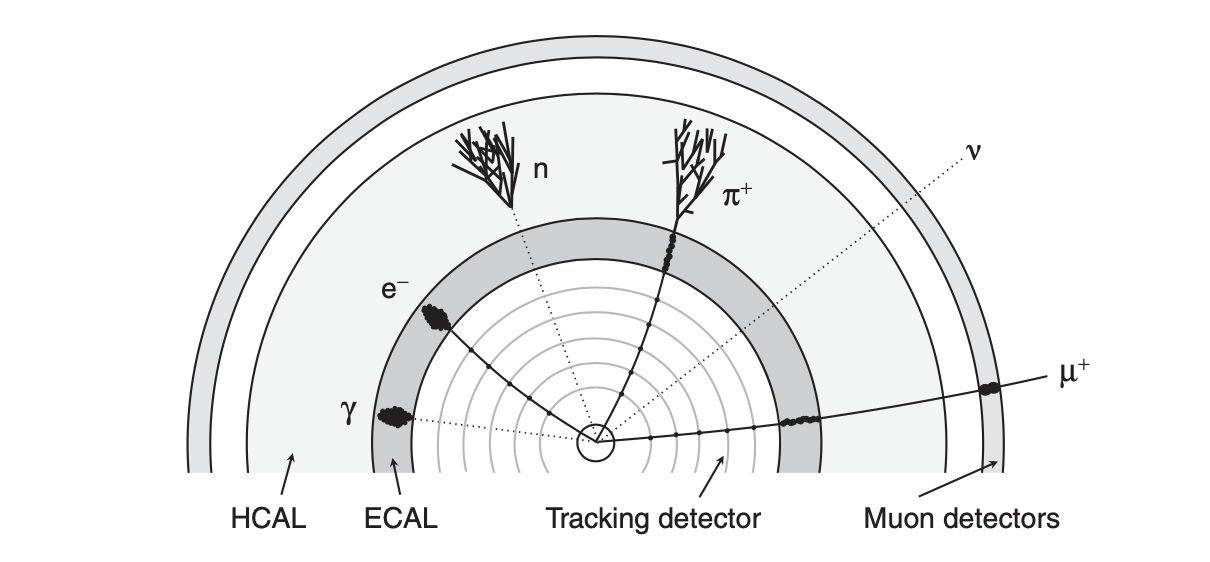
\includegraphics[width=0.7\textwidth]{particle_detection_schematic.png}
    \caption{A schematic representing the particle detection at the CMS detector.
    Hadrons (e.g. $n$, $\pi^{\pm}$) are detected as hadronic showers of particles (jets)
    due to color confinement, and weakly interacting particles such as neutrinos ($\nu$) pass through the
    detector without interaction. Schematic is taken from~\cite{Thomson:2013zua}.}
    \label{fig:particle_detection_cms}
\end{figure}

Since a bunch of protons are collided during each bunch crossing, multiple collision vertices arise
due to multiple interactions within the bunch. The aim of the event reconstruction is to select a primary
collision vertex, which is determined as the vertex containing the largest sum of squared transverse momenta,
$p_{\textrm{T}}^2$, from associated tracks \cite{cms:phase2_upgrade}.
Tracks and energy content from the rest of the vertices are very commonly referred as pileup (PU). With the assignment of the
primary vertex, charged particles can be filtered out from the main event if their tracks are found to be originating 
from a non-primary vertex. This allows to reduce the PU contribution in the reconstructed event. 

In the following subsections, details of how different physics objects are reconstructed will be discussed. To aid the
discussion, signal region (SR) refers to the set of selections used to collect VBF $\hinv$ signal events,
and control regions (CR) refer to the set of selections used to measure and constrain the dominant background yields
in the signal region.

\subsection{Jets}
\label{sec:objects_jets}

A typical jet consists of a shower of hadrons generated by a single quark or gluon.
In this analysis, jets are reconstructed by clustering reconstructed particles
using the anti-$k_{T}$ algorithm~\cite{Cacciari:2008gp}. Jets are
clustered with a distance parameter of $R = 0.4$ and are referred to as AK4
jets. Prior to clustering, charged particles whose tracks are found to be associated
with a non-primary vertex is removed to reduce the energy contributions from other
vertices. This technique is referred to as charged hadron subtraction (CHS)~\cite{CMS:2014ata}. 

Jet momentum is determined as the vector sum of all particle momenta
in the jet, and is found from simulation to be within 5 to 10\% of the
true momentum over the full $\pt$ spectrum and detector acceptance. 
A set of jet energy corrections are applied to correct the jet momenta for various effects,
and bring the reconstructed jet energy to the simulated jet energy ratio closer to $1$.
First, jet energies are further corrected for PU effects, mostly coming from neutral 
particles in the jet after the application of CHS, by using an event-by-event energy density estimation
to derive an offset energy to subtract from the jet energy.
After this, jet momenta are further corrected by using corrections derived from events
where a jet recoils against a well-identified object, including $Z(\ell\ell)\;+$ jet and
$\gamma\;+$ jet events~\cite{Khachatryan:2016kdb}. 
For the analysis that will be explained in this thesis, the
Summer19UL17\_V5 and Summer19UL18\_V5 versions of
the jet energy corrections are used for the 2017 and 2018 datasets,
respectively~\cite{JME:JECRecommendations}. On top of the jet energy corrections,
jet energy resolution (JER) corrections are also applied to correct for differences of 
jet resolution between data and simulation.

The AK4 jets used in this analysis are required to pass the 
loose identification criteria \cite{CMS:JME_jetId}, and AK4 jets with $\pt < 50$ GeV 
must pass the pileup identification (ID) criteria \cite{CMS:JME_jetPuID}. 
Pileup ID criteria aims to reduce the contribution from
pileup by removing jets from the event which contain a large amount of energy from secondary vertices
within the bunch crossing.

% In addition to the pileup ID requirement, jet energy resolution (JER) corrections are applied to all AK4 jets. 
% Application of this correction on all jets is observed to improve the jet modeling, especially at the region near $|\eta| = 2.9$. 
% The effect of JER corrections is shown in Fig.~\ref{fig:jer_correction}, where the $\eta$ distribution is plotted
% for the second-highest $p_{T}$ (subleading) jet in the event, with and without the JER corrections applied.

% \begin{figure}[htb]
%     \begin{minipage}[t]{\linewidth}\centering
%         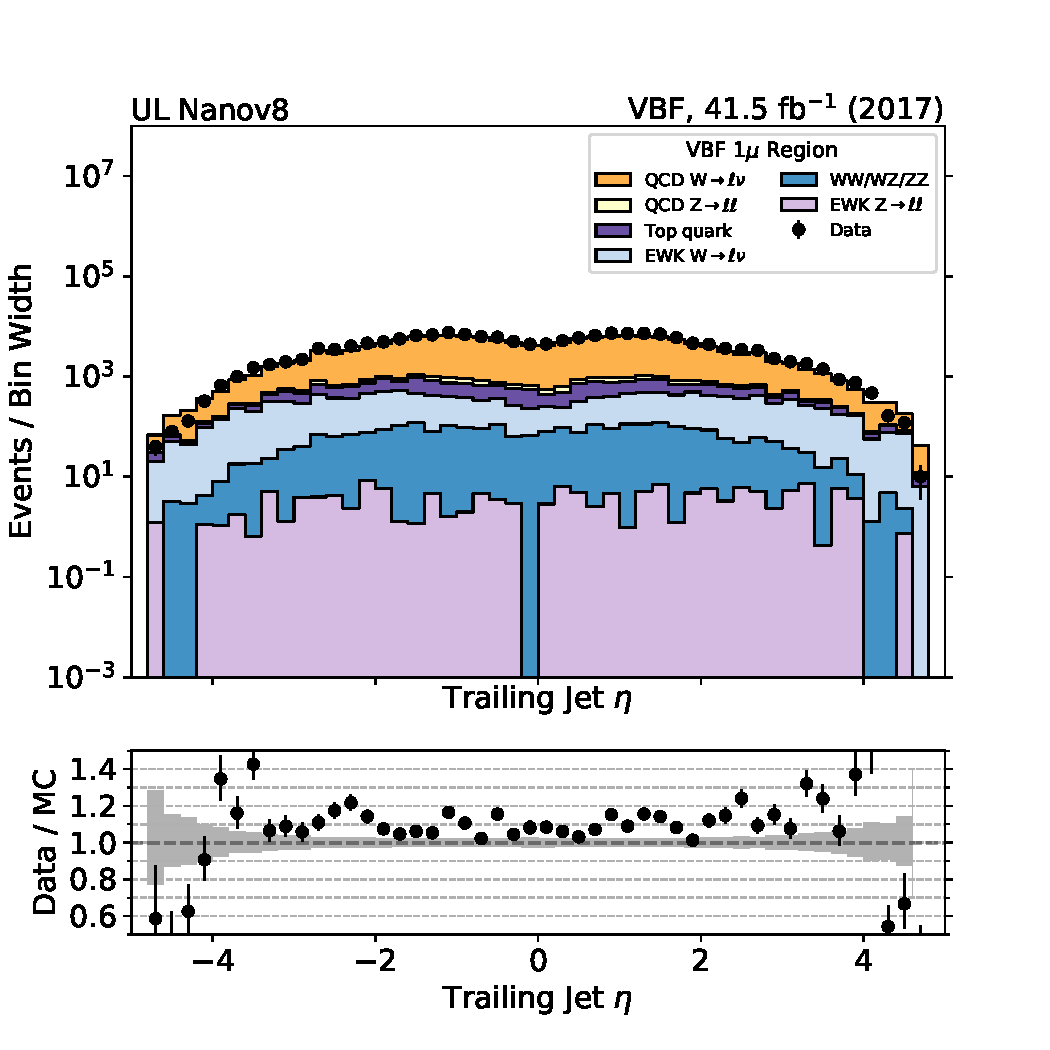
\includegraphics[width=0.45\textwidth]{DataMC/JERImpact/cr_1m_vbf_data_mc_ak4_eta1_2017_withJER.pdf}
%         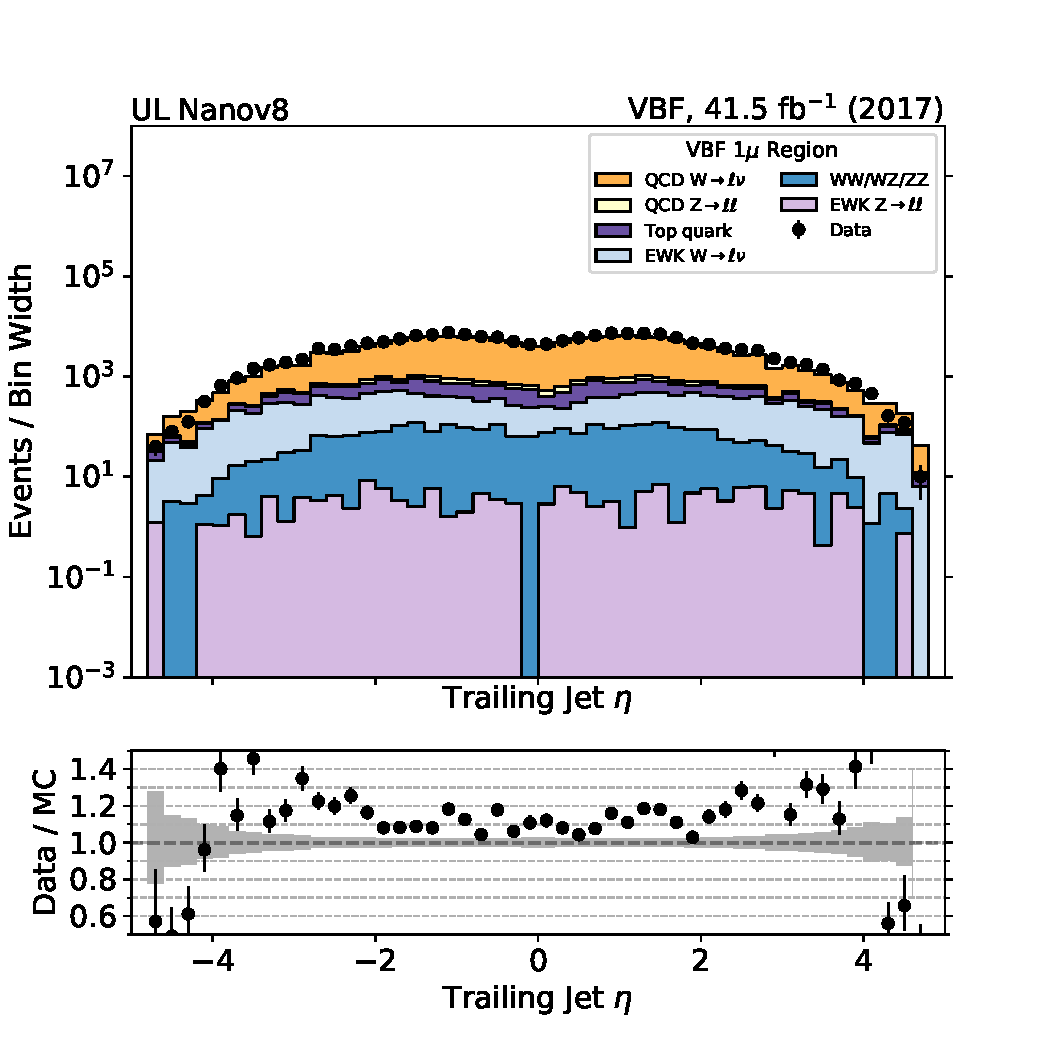
\includegraphics[width=0.45\textwidth]{DataMC/JERImpact/cr_1m_vbf_data_mc_ak4_eta1_2017_noJER.pdf}
%     \end{minipage}
%     \caption{Subleading AK4 jet $\eta$ distribution in single muon control region with JER corrections applied (left) 
%     and without JER corrections applied (right).}
%     \label{fig:jer_correction}
% \end{figure}

In addition, jet-lepton overlap cleaning is done by removing any AK4 jet that is within a cone of radius
$\Delta R = \sqrt{\Delta \eta^2 + \Delta \phi^2} = 0.4$ surrounding a lepton or a photon. Only lepton and 
photon candidates satisfying the object criteria described below are considered during the cleaning.
Lastly, if the leading or the subleading jet is found to be within the tracker coverage (\textit{i.e.,} $|\eta| < 2.5$),
constraints on the charged hadron and neutral hadron energy fractions of the jet ($R_{\textrm{CHEF}}$, $R_{\textrm{NHEF}}$ respectively) 
are placed such that $R_{\textrm{CHEF}} > 0.1$ and 
$R_{\textrm{NHEF}} < 0.8$. If a jet is found to violate these requirements, it is removed from the event.
These additional requirements aid in rejecting misidentified jets with spuriously low charged hadron 
fractions\footnote{On average, one would expect $\approx 60\%$ of jet energy to be in the form of charged particles
(e.g., from charged pions, $\pi^{\pm}$). Hence a reconstructed jet with $<10 \%$ charged energy fraction is highly unexpected and potentially 
due to misidentification of other particles or detector noise.}.

\subsubsection{b-tagged jets}
\label{subsec:objects_bjets}

Identifying jets that originate from a b quark is important in this analysis, since a b quark is not expected in the
final state of the VBF $\hinv$ signal (Fig.~\ref{fig:vbfhinv_signal_diag}), 
and vetoing events with b jets in the final state allows to remove most of the 
backgrounds originating from top quark production.

In this analysis, jets with $\pt > 20$ GeV and $|\eta| < 2.4$ are identified as b jets according to the
DeepCSV algorithm\footnote{Lifetime of hadrons containing b-quarks are
relatively large, $\tau \sim 1.5$ ps, giving rise to a few milimeters of displacement from the primary vertex
before further decay, hence creating a second, displaced vertex. The b tagging algorithms like DeepCSV make use of
this feature to classify a jet as coming from a b quark or not.}~\cite{Sirunyan:2017ezt}. 
A medium working point is adopted, corresponding to correctly identifying a b jet with a
probability of 80\%, and mis-identifying a light-flavor jet with a probability of 10\%. This working point corresponds to the value of 
DeepCSV tagger to be greater than 0.4506 in 2017, and 0.4168 in 2018.

\subsection{Missing transverse momentum}
\label{subsec:objects_met_recoil}

The vector \ptvecmiss is defined as the imbalance in the transverse
momentum of all particles that interact with the detectors.
Due to momentum conservation in the plane transverse to the beam axis, \ptvecmiss
corresponds to the transverse momentum that is carried by undetected particles such as neutrinos.
Large $\ptvecmiss$ can also imply the observation of a $\hinv$ signal, due to the decay products
of the Higgs boson passing undetected through the detector\footnote{Further discussion
on this can be found in the Introduction chapter, please see Sec.~\ref{subsec:exp_signatures}.}.
Therefore, $\ptvecmiss$ is a key variable in this analysis.   
It is computed as the negative of the vectorial sum of transverse
momenta of all PF candidates and is therefore also referred to as PF \ptvecmiss.
The magnitude of the \ptvecmiss is referred to as \ptmiss.

Minimum energy thresholds in the calorimeters, inefficiencies
in the tracker, nonlinearity of the response of the calorimeter
for hadronic particles can lead to an over- or underestimation of \ptmiss.
The bias on the \ptmiss measurement is reduced by propagating the effect of the jet energy
corrections introduced in Sec.~\ref{sec:objects_jets} according to

\begin{equation}
\ptvecmiss(\mathrm{corr})
=\ptvecmiss - \sum_\mathrm{jets} (\vec{p}_\mathrm{T,jet}({\mathrm{corr}})-\vec{p}_\mathrm{T,jet}) \quad ,
\label{eq:Type1MET}
\end{equation}
where the ``corr'' refers to the energy corrected measurements
of the related objects.
This correction for \ptvecmiss uses jet energy scale corrections
for all corrected jets with $\pt > 15$ GeV that have less than $90 \%$
of their energy deposited in the ECAL. Furthermore, if a muon is found in a
jet, its 4-momentum is subtracted from the 4-momentum of the jet
when performing the correction and is added back to a corrected object.

Since VBF \hinv signal events in this analysis contain only jets and no other 
reconstructed visible candidates in the final state,
\ptmiss is equivalent to the total hadronic momentum in the event that is transverse to the proton-proton collision axis. 
For the leading $\Zvvjets$ and $\Wlvjets$ backgrounds which can result in the same final state 
(described in Sec.~\ref{subsec:sr_vbf_selection}), 
$\ptmiss$ corresponds to the transverse momentum of the $\textrm{Z}$ and $\textrm{W}$ boson, respectively. 
To mimic this behavior in in the control regions of this analysis, the hadronic recoil
$\vec{U}$ is used, which is defined as the sum of the transverse
momenta of all particles except the vector boson (or its decay products).
The hadronic recoil $\vec{U}$ is computed as

\begin{equation}
  \vec{U} = \ptvecmiss + \sum _{i\;\in\;\textrm{leptons, photons}}\ptveci \quad ,
  \label{eq:recoil_def}
\end{equation}
where the sum takes into account the leptons and photons used to define the respective control 
region\footnote{Please see Sec.~\ref{sec:event_selection} for the discussion of all control regions
used in the analysis.}.
As an example, in the control region where $\Zmmjets$ events are collected, the recoil $\vec{U}$ can be
computed as $\vec{U} = \ptvecmiss + \sum_{i\;\in\;\textrm{muons}} \ptveci$, where the sum goes over
the two reconstructed muons, which are the decay products of the $Z$ boson. Here, assumming small $\ptvecmiss$
due to the fact that the final state muons will not result in transverse momentum imbalance, 
$\vec{U} \approx \sum_{i\;\in\;\textrm{muons}} \ptveci \approx \vec{p}_T^{\;Z}$. Hence,
in all regions in the analysis, $\vec{U}$ can be thought of as the transverse momentum of the $Z$, $W$ or $\gamma$ 
boson, depending on the control region being considered.
For the signal region, 
since there are no reconstructed leptons in the final state, it should be noted that the sum term
in Eq.~\ref{eq:recoil_def} will be $0$, hence making $\vec{U} = \ptvecmiss$ for the signal 
region\footnote{But still, please note that $\vec{U} \approx \vec{p}_T^{\;V}$ condition holds true in the
signal region for $\Vjets$ backgrounds, where $V = Z, W$. Hence the definition of hadronic recoil $\vec{U}$ is consistent
across all regions in the analysis.}.

% The uncertainty of \ptmiss has a strong dependence on the
% event topology. Therefore, the uncertainty on \ptmiss is often factorized into its components of
% jets, leptons and unclustered energy. Each sub-component is then varied
% within its scale and resolution uncertainty.

In addition to the events with genuine $\ptmiss$, such as $\Zvvjets$, 
anomalous high-\ptmiss events can also appear due to various phenomena.
In the ECAL, spurious deposits may appear due to particles striking
sensors in the ECAL photodetectors, or from real showers with non-collision
origins such as those caused by beam halo particles. Dead ECAL cells can cause real
energy to be missed, again leading to a spurious imbalance.
In the HCAL, spurious energy can arise due to  noise in the hybrid
photodiode and readout box  electronics, as well as
direct particle interactions with  the light guides and
photomultiplier tubes of the forward calorimeter. 
A number of filters has been developed by the POG/DPG groups to identify and suppress anomalous high
\ptmiss events~\cite{CMS-JME-TWIKI-FILTER}. The recommended filters are listed in Tab.~\ref{tab:metfilters} and are applied in the analysis.

\begin{table}[ht!]
    \centering
    \small
    \def\arraystretch{1.5}
    \caption{The \ptmiss filters recommended by the JME POG~\cite{CMS-JME-TWIKI-FILTER}. 
    The recommendations apply to both 2017 and 2018. Except for the bad super cluster filter (``EE badSC''), all filters are applied both in data and simulation (MC).}
    \begin{tabular}{p{5cm} p{7cm} p{2cm} }
        \hline
        \hline
                                           &                                                                     \\
        Filter                             & Name in input dataset                    & Applied in data (MC)     \\\hline
        Primary vertex filter              & Flag\_goodVertices                       & \checkmark  (\checkmark) \\
        Beam halo filter                   & Flag\_globalSuperTightHalo2016Filter     & \checkmark  (\checkmark) \\
        HBHE noise filter                  & Flag\_HBHENoiseFilter                    & \checkmark  (\checkmark) \\
        HBHEiso noise filter               & Flag\_HBHENoiseIsoFilter                 & \checkmark  (\checkmark) \\
        ECAL TP filter                     & Flag\_EcalDeadCellTriggerPrimitiveFilter & \checkmark  (\checkmark) \\
        Bad PF Muon Filter                 & Flag\_BadPFMuonFilter                    & \checkmark  (\checkmark) \\
        EE badSC noise filter              & Flag\_eeBadScFilter                      & \checkmark  ($\times$)     \\
        ECAL bad calibration filter update & Flag\_ecalBadCalibFilter               & \checkmark  (\checkmark) \\
        \hline
    \end{tabular}

    \label{tab:metfilters}
\end{table}

\subsection{Leptons}

\subsubsection{Muons}
\label{subsec:muons}

Muons are reconstructed by combining information from silicon tracker detector and the muon detection system
\cite{cms:muon_paper}. Requirements for a good-quality muon object include the fit quality of the
muon track, and its consistency with the primary vertex in the event. All muons considered in this
analysis have $\pt > 10$ GeV and $|\eta| < 2.4$ (\textit{i.e.,} they are reconstructed within the tracker range).

Two types of muon identification are used for this analysis, which are termed as loose and tight muons \cite{CMS-MUO-TWIKI-IDLOOSE,CMS-MUO-TWIKI-IDTIGHT}.
Loose muon identification is used to identify muons in the signal region and veto them\footnote{This selection is due to the fact that
final state muons are not expected in VBF $\hinv$ signal events. As explained later in Sec.~\ref{subsec:sr_vbf_selection}, this veto
helps suppressing background processes such as $\Wmnjets$ and $\Zmmjets$.}. 
Tight muon identification, on the other hand,
has more strict quality conditions and are used to identify good quality muons in $\textrm{W}(\mu \nu)$ and $\textrm{Z}(\mu \mu)$ control regions.

Loose muon objects must pass the following requirements \cite{CMS-MUO-TWIKI-IDLOOSE}:

\begin{itemize}
    \item Must be reconstructed as a muon by the Particle Flow (PF) algorithm
    \item Must have $\pt > 10$ GeV and $|\eta| < 2.4$
\end{itemize}

Tight muons pass all the requirements of loose muons, together with passing these additional muon quality requirements \cite{CMS-MUO-TWIKI-IDTIGHT}:

\begin{itemize}
    \item Must have $p_T > 20$ GeV and $|\eta| < 2.4$
    \item Normalized $\chi^2$ of the muon track fit $<$ 10
    \item At least one muon chamber hit must be included in the muon track fit
    \item Muon segments required in at least two muon stations
    \item Muon track must have transverse impact parameter $d_{xy} < $ 2~mm w.r.t. the primary vertex
    \item The longitudinal distance of the tracker track w.r.t. the primary vertex must be $d_z < $ 5~mm
    \item Number of pixel hits $>$ 0
    \item Cut on number of tracker layers with hits $>$ 5
\end{itemize}

In addition to the requirements listed above, an energy isolation requirement is imposed on the muons. An isolation variable 
is computed based on the sum of energies of nearby PF candidates, within $\Delta R < 0.4$ of the muon. This isolation
variable is then used to select muons that are relatively isolated from other physical objects. This isolation variable
is required to be less than $0.25$ for loose muons, and less than $0.15$ for tight muons.


\subsubsection{Electrons}
\label{subsec:electrons}

Electrons are reconstructed using the information from the tracker and the ECAL detector \cite{cms:elepho_paper}. All electrons
considered in this analysis have $\pt > 10$ GeV and $|\eta| < 2.5$.

Similar to the case of muons, two types of identification are used for electrons, which are labeled as veto and tight electrons.
Veto electrons are used to identify electrons in the signal region and veto events containing such 
electrons\footnote{Similar to the case of muons, such a veto helps suppressing background processes such as
$\Wevjets$ and $\Zeejets$ in the signal region.}. 
Tight electrons, which have tighter
quality cuts, are used to identify electrons in $\textrm{W}(\textrm{e} \nu)$ and $\textrm{Z}(\textrm{ee})$ control regions.

The quality requrements for veto and tight electron objects are different for electrons reconstructed in the barrel region
($|\eta| < 1.479$) and in the endcap region ($|\eta| > 1.479$). The details of the quality requirements are listed in Tables \ref{tab:veto_electron_def_barrel},
\ref{tab:tight_electron_def_barrel}, \ref{tab:veto_electron_def_endcap} and \ref{tab:tight_electron_def_endcap}.

\begin{table}[htbp]
\centering
\def\arraystretch{1.2}

\begin{tabular}{|l|c|}
    \hline\hline
    Quantity & Requirement \\\hline
    Full 5x5 $\sigma_{i\eta i\eta}$ &  $< 0.0126$ \\
    $|\Delta\eta_{\mathrm{seed}}|$ & $< 0.00463$  \\
    $|\Delta\phi_{\mathrm{In}}|$ & $< 0.148$ \\
    \textit{H/E} & $<$ 0.05+1.16/$E_{\mathrm{SC}}$+0.0324$\rho$/$E_{\mathrm{SC}}$ \\
    Relative Isolation With EA & $<$ 0.198+0.506/$\pt$ \\
    $|$1/\textit{E}-1/\textit{p}$|$ & $< 0.209$ \\
    Expected Missing Inner Hits & $\leq$ 2 \\
    Pass conversion veto & yes \\
    \hline\hline
\end{tabular}
\caption{Requirements used to define veto electrons in the barrel region ($|\eta| < 1.479$).}
\label{tab:veto_electron_def_barrel}
\end{table}

\begin{table}[htbp]
\centering
\def\arraystretch{1.2}
\begin{tabular}{|l|c|}
    \hline\hline
    Quantity & Requirement \\\hline
    Full 5x5 $\sigma_{i\eta i\eta}$ &  $< 0.0104$ \\
    $|\Delta\eta_{\mathrm{seed}}|$ & $< 0.00255$  \\
    $|\Delta\phi_{\mathrm{In}}|$ & $< 0.022$ \\
    \textit{H/E} & $<$ 0.026+1.15/$E_{\mathrm{SC}}$+0.0324$\rho$/$E_{\mathrm{SC}}$ \\
    Relative Isolation With EA & $<$ 0.0287+0.506/$\pt$ \\
    $|$1/\textit{E}-1/\textit{p}$|$ & $< 0.159$ \\
    Expected Missing Inner Hits & $\leq$ 1 \\
    Pass conversion veto & yes \\
    \hline\hline
\end{tabular}
\caption{Requirements used to define tight electrons in the barrel region ($|\eta| < 1.479$).}
\label{tab:tight_electron_def_barrel}
\end{table}

\begin{table}[htbp]
\centering
\def\arraystretch{1.2}
\begin{tabular}{|l|c|}
    \hline\hline
    Quantity & Requirement \\\hline
    Full 5x5 $\sigma_{i\eta i\eta}$ &  $< 0.0457$ \\
    $|\Delta\eta_{\mathrm{seed}}|$ & $< 0.00814$  \\
    $|\Delta\phi_{\mathrm{In}}|$ & $< 0.19$ \\
    \textit{H/E} & $<$ 0.05+2.54/$E_{\mathrm{SC}}$+0.183$\rho$/$E_{\mathrm{SC}}$ \\
    Relative Isolation With EA & $<$ 0.203+0.963/$\pt$ \\
    $|$1/\textit{E}-1/\textit{p}$|$ & $< 0.132$ \\
    Expected Missing Inner Hits & $\leq$ 3 \\
    Pass conversion veto & yes \\
    \hline\hline
\end{tabular}
\caption{Requirements used to define veto electrons in the endcap region ($|\eta| > 1.479$).}
\label{tab:veto_electron_def_endcap}
\end{table}

\begin{table}[htbp]
\centering
\def\arraystretch{1.2}
\begin{tabular}{|l|c|}
    \hline\hline
    Quantity & Requirement \\\hline
    Full 5x5 $\sigma_{i\eta i\eta}$ &  $< 0.0353$ \\
    $|\Delta\eta_{\mathrm{seed}}|$ & $< 0.00501$  \\
    $|\Delta\phi_{\mathrm{In}}|$ & $< 0.0236$ \\
    \textit{H/E} & $<$ 0.0188+2.06/$E_{\mathrm{SC}}$+0.183$\rho$/$E_{\mathrm{SC}}$ \\
    Relative Isolation With EA & $<$ 0.0445+0.963/$\pt$ \\
    $|$1/\textit{E}-1/\textit{p}$|$ & $< 0.0197$ \\
    Expected Missing Inner Hits & $\leq$ 1 \\
    Pass conversion veto & yes \\
    \hline\hline
\end{tabular}
\caption{Requirements used to define tight electrons in the endcap region ($|\eta| > 1.479$).}
\label{tab:tight_electron_def_endcap}
\end{table}

In addition to the requirements listed in the tables above, electrons are cross-cleaned against the muons
within $\Delta R < 0.3$.

\subsubsection{Taus}

Hadronically decaying $\tau$ leptons are required to pass identification criteria
using the DeepTau algorithm~\cite{CMS-DP-2019-033}. In addition, $\tau$ candidates are required to be isolated from other activity in the
event. The isolation requirement is computed by summing the \pt of the charged PF
candidates and PF photon candidates within an isolation cone of $\Delta R = 0.5$,
around the tau candidate direction. 
% The other charged lepton candidates and photon candidates associated with the
% tau candidate are removed from this sum and further described in Ref.~\cite{Khachatryan:2015dfa}.
The ``VVLoose'' isolation working point~\cite{taupog_twiki} is employed in this analysis
for tau candidates with $\pt > 20$ GeV within $|\eta| < 2.3$. $\tau$ candidates within $\Delta R = 0.4$ of 
an identified veto electron or loose muon are rejected. If hadronically decaying taus are reconstructed within
an event that satisfy the conditions mentioned above, the event is rejected from the analysis to suppress 
backgrounds coming from the hadronic decays of tau leptons. 

\subsection{Photons}
\label{subsec:photons}

Photon candidates are reconstructed from energy deposits in the ECAL using algorithms
that constrain the clusters to the size and shape expected from a photon~\cite{CMS:EGM-14-001}.
The identification of the candidates is based on shower-shape and isolation variables.
For isolated photons, scalar sums of the \pt of PF candidates within a cone of $\Delta R < 0.3$
around the photon candidate are required to be below the bounds defined. Only the PF candidates
that do not overlap with the electromagnetic shower of the candidate photon are included in the isolation sums.

Similar to electrons and muons, two candidate definitions are employed for photons. Loose photons are used to reject
events with reconstructed photons in the signal region. These photons are required to pass the EGamma POG loose identification criteria~\cite{CMS-EGM-TWIKI-GAMID},
have $\pt > 15$ GeV and be within $|\eta|<2.5$. The exact identification criteria for loose photons in barrel and endcap 
are summarized in Tables.~\ref{tab:PhotonIDLooseBarrel} and~\ref{tab:PhotonIDLooseEndcap}, respectively.
Tight photons are used to identify photon objects in the dedicated photon control region. 
These photons are explicitly required to be in the barrel ($|\eta|<1.479$), and have $\pt>230$ GeV. The identification criteria for tight photons
are summarized in Table~\ref{tab:PhotonIDTight}.

\begin{table}[htb!]
    \centering
    \small
    \def\arraystretch{1.2}
    \begin{tabular}{l c}
    \hline
    Variable                                   &  Selection       \\
                                               &  Barrel ($|\eta|<1.479$) \\
    \hline
    \hline
    Full 5x5 $\sigma_{i\eta i\eta}$            & $< 0.0106 $    \\
    \textit{H/E}                               & $<  0.04596 $    \\
    charged hadron isolation                   & $< 1.694 $     \\
    neutral hadron isolation                   & $< 24.032 + 0.01512 \pt+2.259 10^{-5} {\pt}^2$ \\
    photon isolation                           & $< 2.876 + 0.004017 \pt$  \\
    Conversion safe electron veto              & Yes           \\
    \hline
    \end{tabular}
    \caption{Loose photon identification criteria for photons in the barrel. These photons must also have $\pt > 15$ GeV.}
    \label{tab:PhotonIDLooseBarrel}
\end{table}

\begin{table}[htb!]
    \centering
    \small
    \def\arraystretch{1.2}
    \begin{tabular}{l c}
    \hline
    Variable                                   &  Selection       \\
                                               &  Endcap ($1.479<|\eta|<2.5$)  \\
    \hline
    \hline
    Full 5x5 $\sigma_{i\eta i\eta}$            & $< 0.0272 $    \\
    \textit{H/E}                               & $< 0.0590 $    \\
    charged hadron isolation                   & $< 2.089 $     \\
    neutral hadron isolation                   & $< 19.722 + 0.0117 \pt+2.3 10^{-5} {\pt}^2$ \\
    photon isolation                           & $< 4.162 + 0.0037 \pt$  \\
    Conversion safe electron veto              & Yes           \\
    \hline
    \end{tabular}
    \caption{Loose photon identification criteria for photons in the endcap. These photons must also have $\pt > 15$ GeV.}
    \label{tab:PhotonIDLooseEndcap}
\end{table}

\begin{table}[htb!]
    \centering
    \small
    \def\arraystretch{1.2}
    \begin{tabular}{l c}
    \hline
    Variable                                   &  Selection       \\
                                               &  Barrel  \\
    \hline
    \hline
    Full 5x5 $\sigma_{i\eta i\eta}$            & $<  0.01015  $ \\
    \textit{H/E}                               & $<  0.02197  $   \\
    charged hadron isolation                   & $< 1.141  $     \\
    neutral hadron isolation                   & $< 1.189  + 0.01512 \pt+2.259 10^{-5} {\pt}^2$ \\
    photon isolation                           & $< 2.08 + 0.004017 \pt$  \\
    Conversion safe electron veto              & Yes           \\
    \hline
    \end{tabular}
    \caption{Tight photon identification criteria. The criteria are only given for the barrel region since endcap photons are not 
    considered in the analysis.}
    \label{tab:PhotonIDTight}
\end{table}

\subsubsection{Photon purity}
\label{subsec:photonpurity}

Photons are reconstructed from ECAL clusters, and can be discriminated from other sources of ECAL deposits due 
to the properties of the cluster, as well as their lack of other associated signatures such as tracks or HCAL 
deposits. This discrimination is not perfect, however, and in some cases, non-photon objects will incorrectly be 
identified as photons, which in this text are also referred to as ``fake photons''.
The leading source of fake photons is QCD production of multijet events, where 
a jet is misidentified as a photon. The QCD process is relevant mainly because of its large cross-section, which yields non-negligible 
contributions to the photon selection even if the per-jet probability of misreconstruction is small.

To estimate the fake contribution to the photon control region, a purity measurement is performed. The photon purity is 
defined as the fraction of reconstructed photons that is actually due to an isolated photon from the hard scattering event, 
as opposed to a fake. The purity is obtained from a template fit to the distribution of the \sieie variable in data, where 
\sieie variable represents the width of the ECAL shower in the $\eta$ direction. Due to the different shower behavior of 
photons and hadrons, the \sieie distribution shows characteristically different behavior between these two classes of 
reconstructed photons: Real photons show a large peak with a cut-off at around $\sieie\approx0.01$, while fake photons will 
have a smaller peak (stemming from actual photons inside jets), and an additional non-peaking bulk region at larger 
\sieie (stemming from hadrons interacting in the ECAL). The inputs to the fit are defined as follows:

\begin{itemize}
\item Photons in data are selected by applying the same identification criteria as for the tight selection defined above, 
with the exception of the \sieie requirement. By removing this requirement, the full \sieie distribution can be observed.

\item A real photon template is obtained from $\gamma +$ jets Monte Carlo (MC) simulation. The same identification criteria are applied as in data.

\item A fake photon template is obtained from data. In this case, the identification criteria are modified by requiring that 
at least one of the isolation criteria is not passed. Therefore, the photons in this template represent reconstructed photons inside jets,
(\textit{i.e.,} ``fake photons").

\end{itemize}

The templates are derived in separate bins of the photon $\pt$ and the measurement is performed separately for 2017 and 2018. 
Events are selected using the following criteria:

\begin{itemize}
    \item At least one jet with $\pt>100$ GeV and $|\eta|<2.4$, which is not overlapping with a photon of interest.
    \item The event must pass the HLT\_Photon200 trigger, which requires a photon with $\pt > 200$ GeV to be reconstructed at the HLT level.
    \item The event must pass the offline MET filters, and have $\ptmiss < 60$ GeV.
\end{itemize}

The fits are shown in Figs.~\ref{fig:purity_fits_2017} and~\ref{fig:purity_fits_2018}. The resulting impurity values as a function of photon \pt 
are shown in Fig.~\ref{fig:purity_result}. While the fits are performed in the range of $0.04<\sieie<0.15$, the purity is evaluated only taking 
into account the contributions with $\sieie<0.01$, which is the requirement posed in the identification criteria used in the analysis (see Tab.~\ref{tab:PhotonIDTight}).  
Overall, good fit performance is observed and the impurity is found to range between $1\%$ and $4\%$, with a decreasing trend with increasing photon \pt. 
Residual differences between the best fit and the data appear because the template shapes do not match the data shapes perfectly. To take this 
effect into account, the measurement is repeated with four alternative binning schemes that range from being very fine to very coarse and are shown in 
Fig.~\ref{fig:purity_binning}. By varying the binning choice, the effect of shape differences can be amplified or mitigated, and its impact on the 
final impurity values can be tested. The spread of the resulting values per bin is found to be small and a 25\% uncertainty is assigned to the impurity 
and thus the QCD background estimate. For application in the analysis, the nominal impurity values are interpolated using an exponential function fit.

\begin{figure}[htbp]
    \centering
        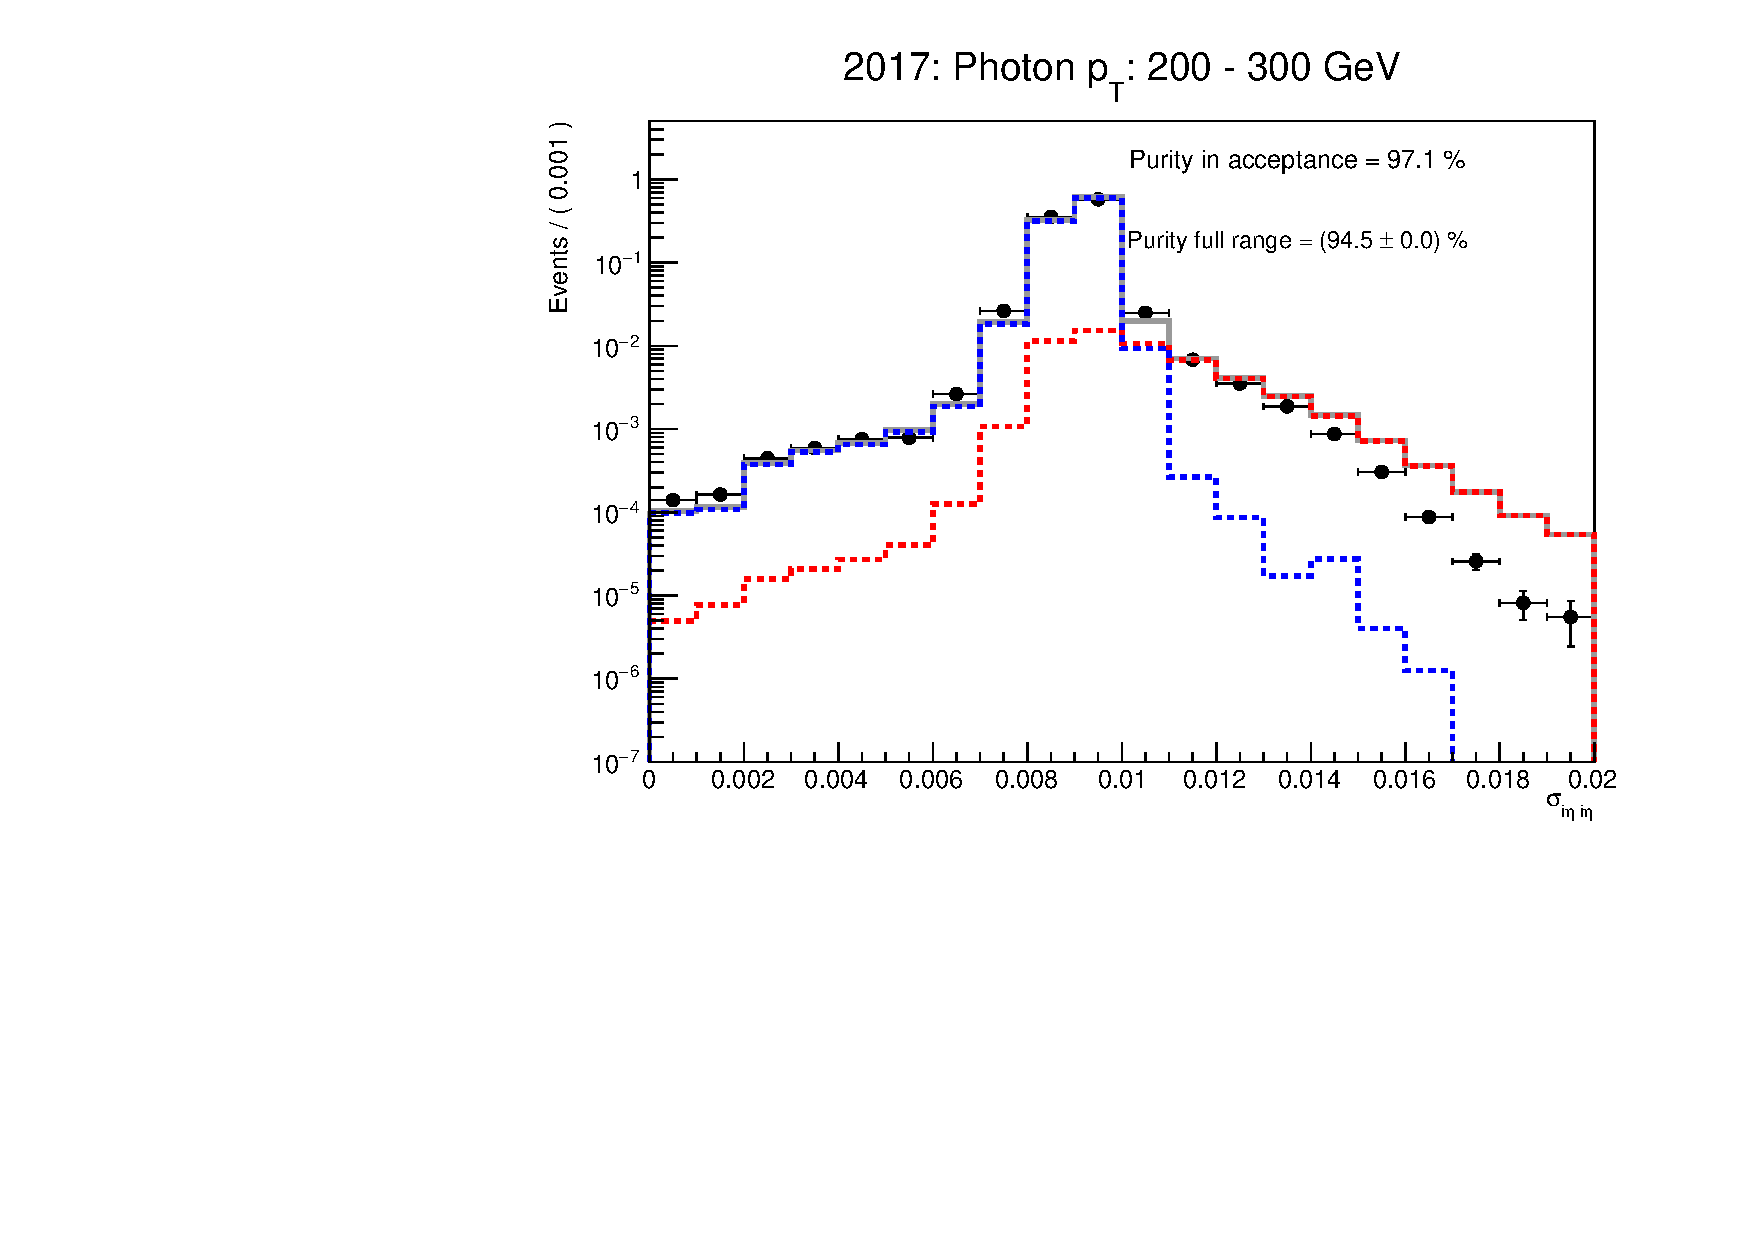
\includegraphics[width=0.45\textwidth]{PhotonPurity/fit_2017_pt200-300_nominal.pdf}
        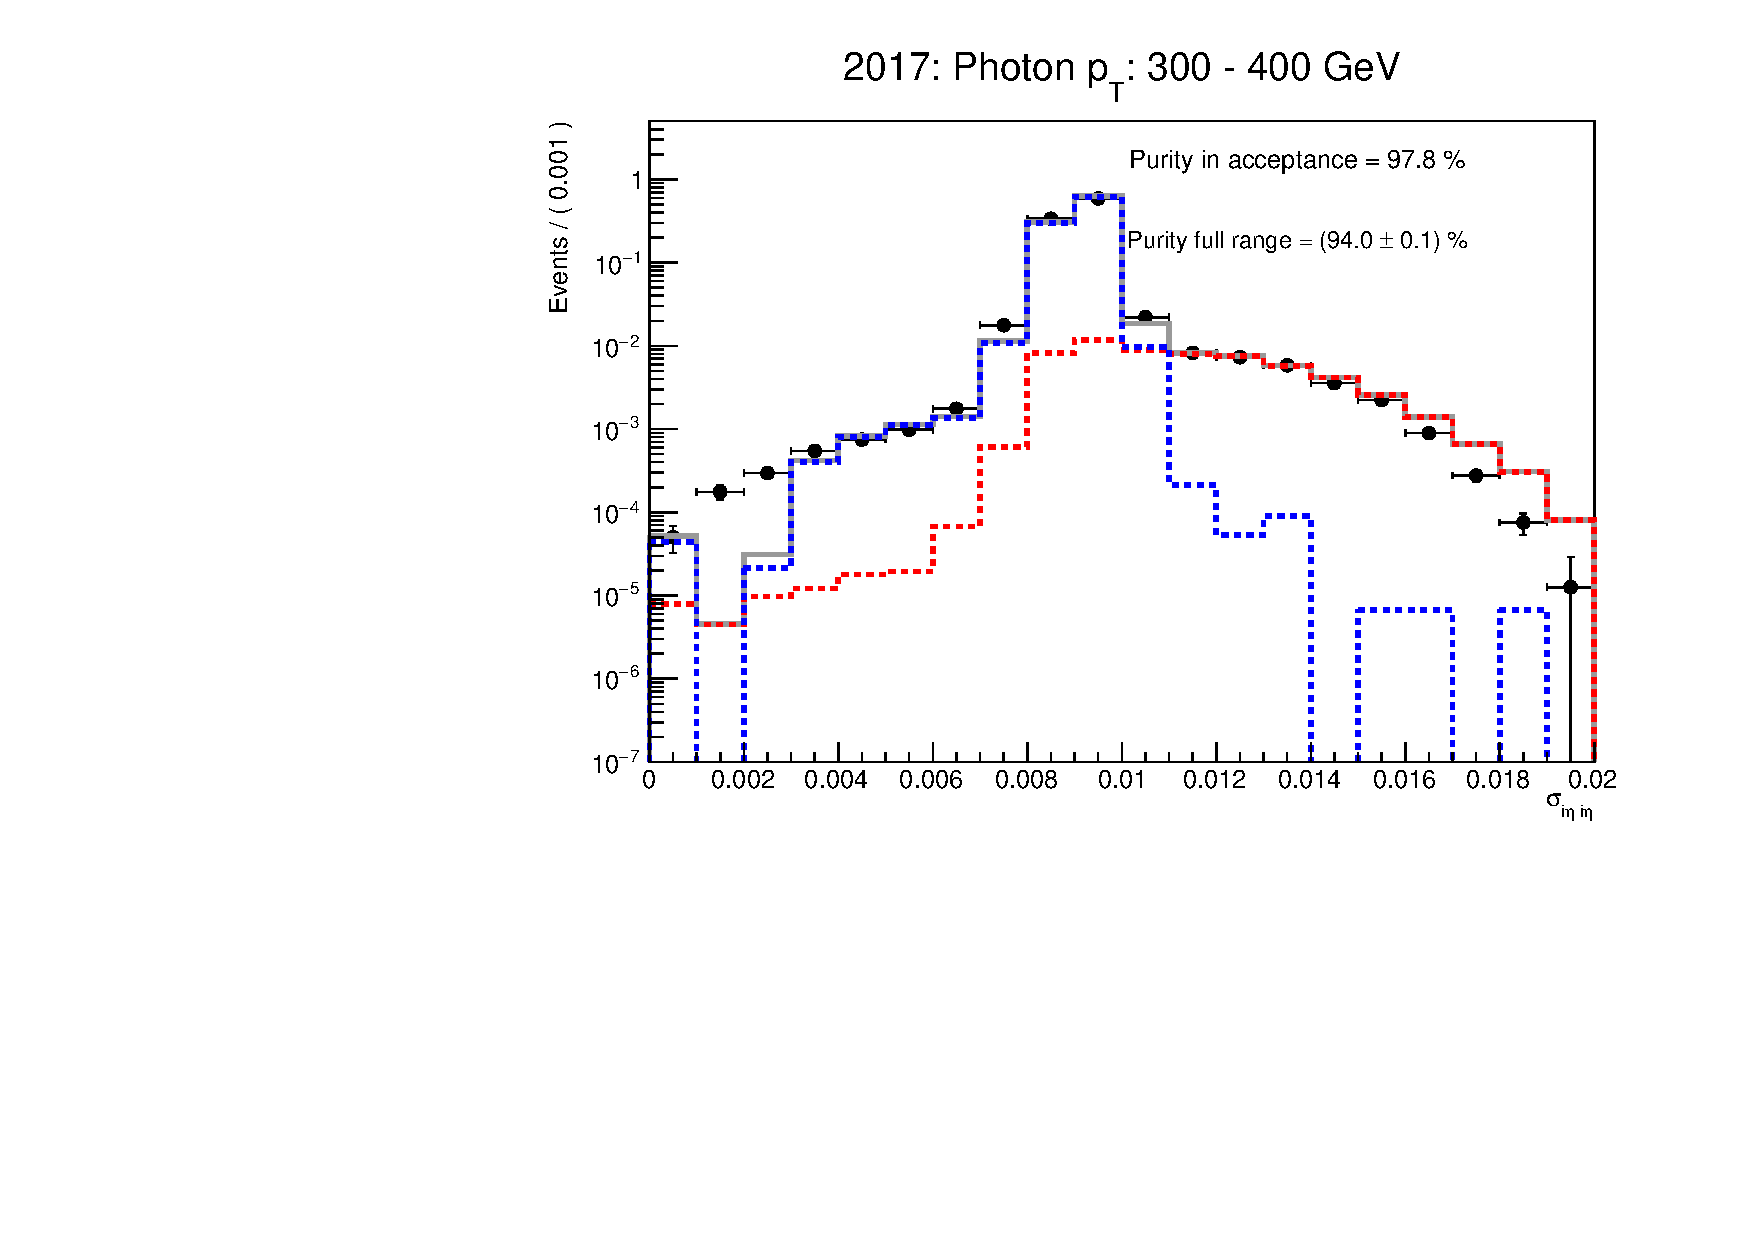
\includegraphics[width=0.45\textwidth]{PhotonPurity/fit_2017_pt300-400_nominal.pdf}
        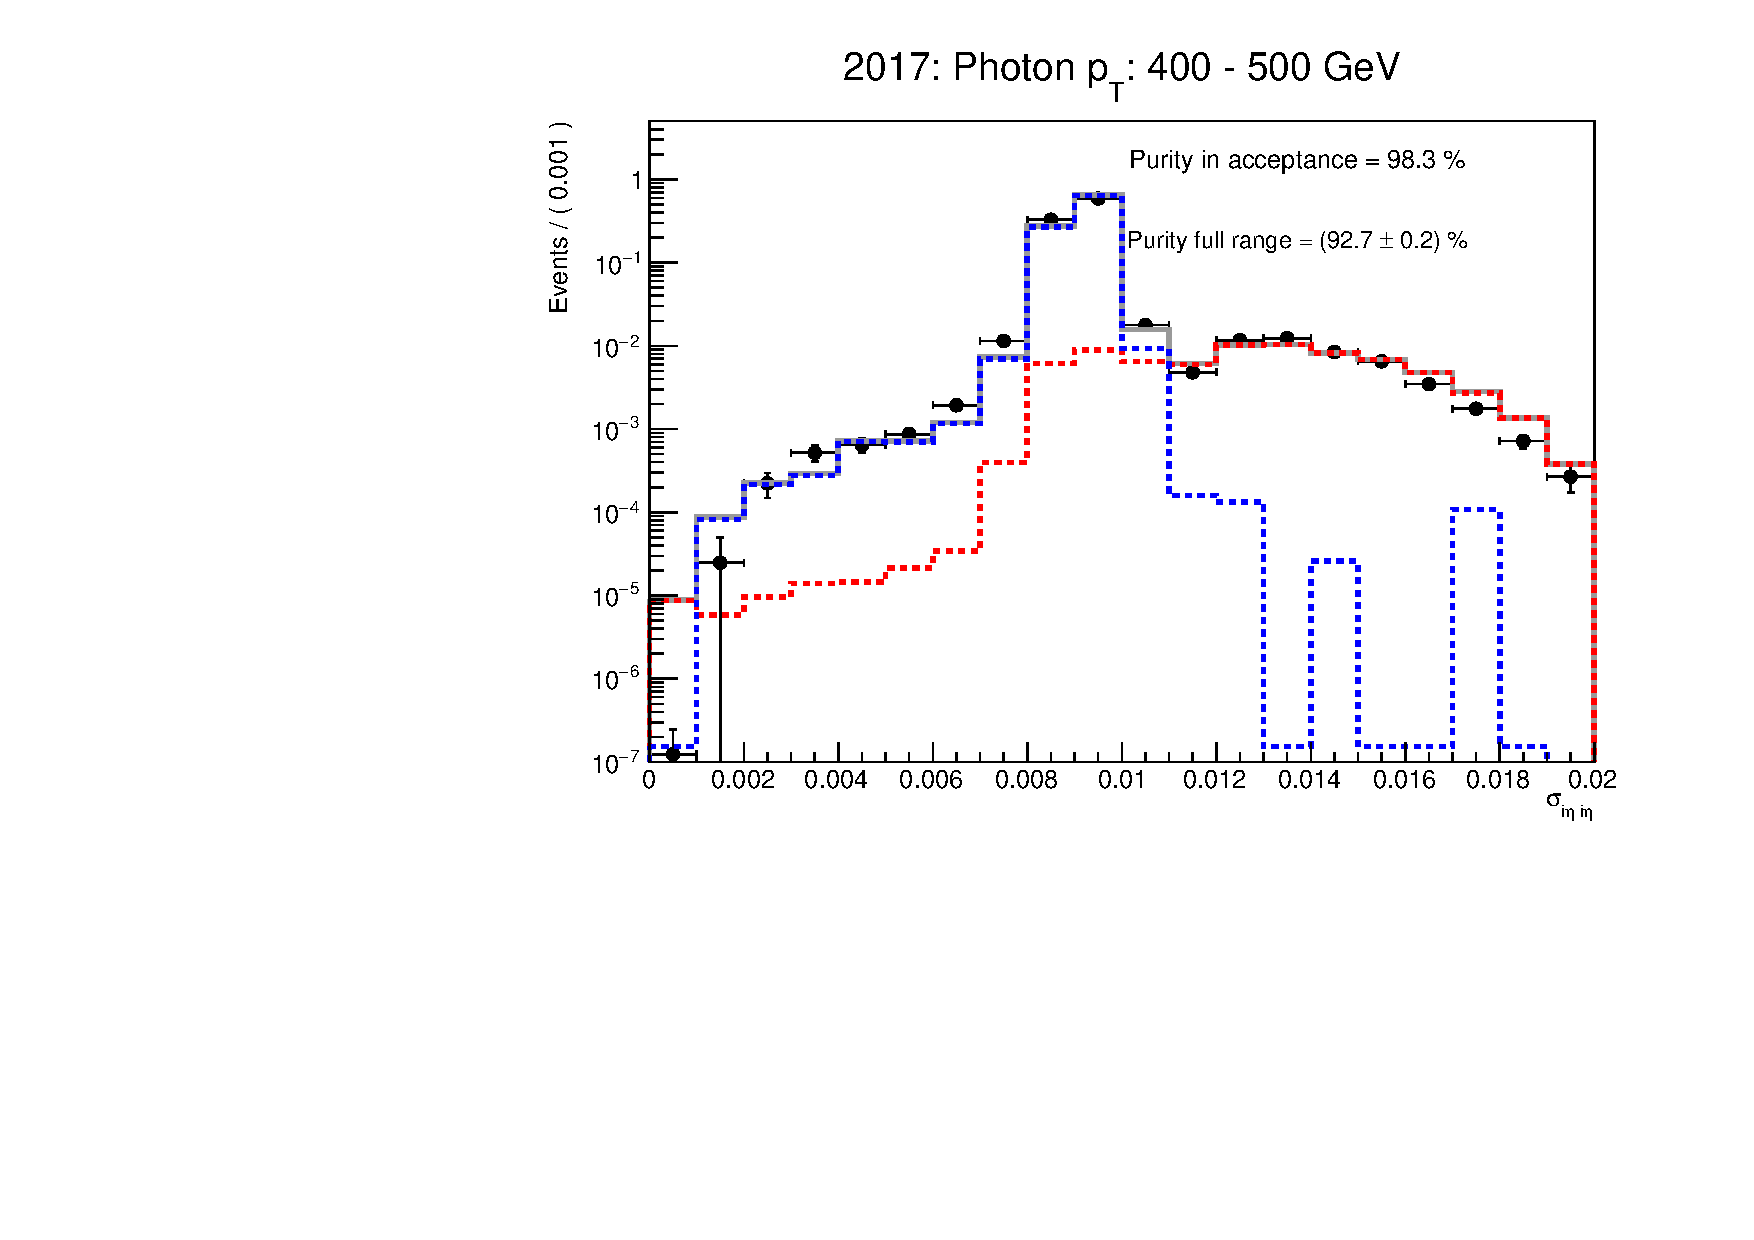
\includegraphics[width=0.45\textwidth]{PhotonPurity/fit_2017_pt400-500_nominal.pdf}
        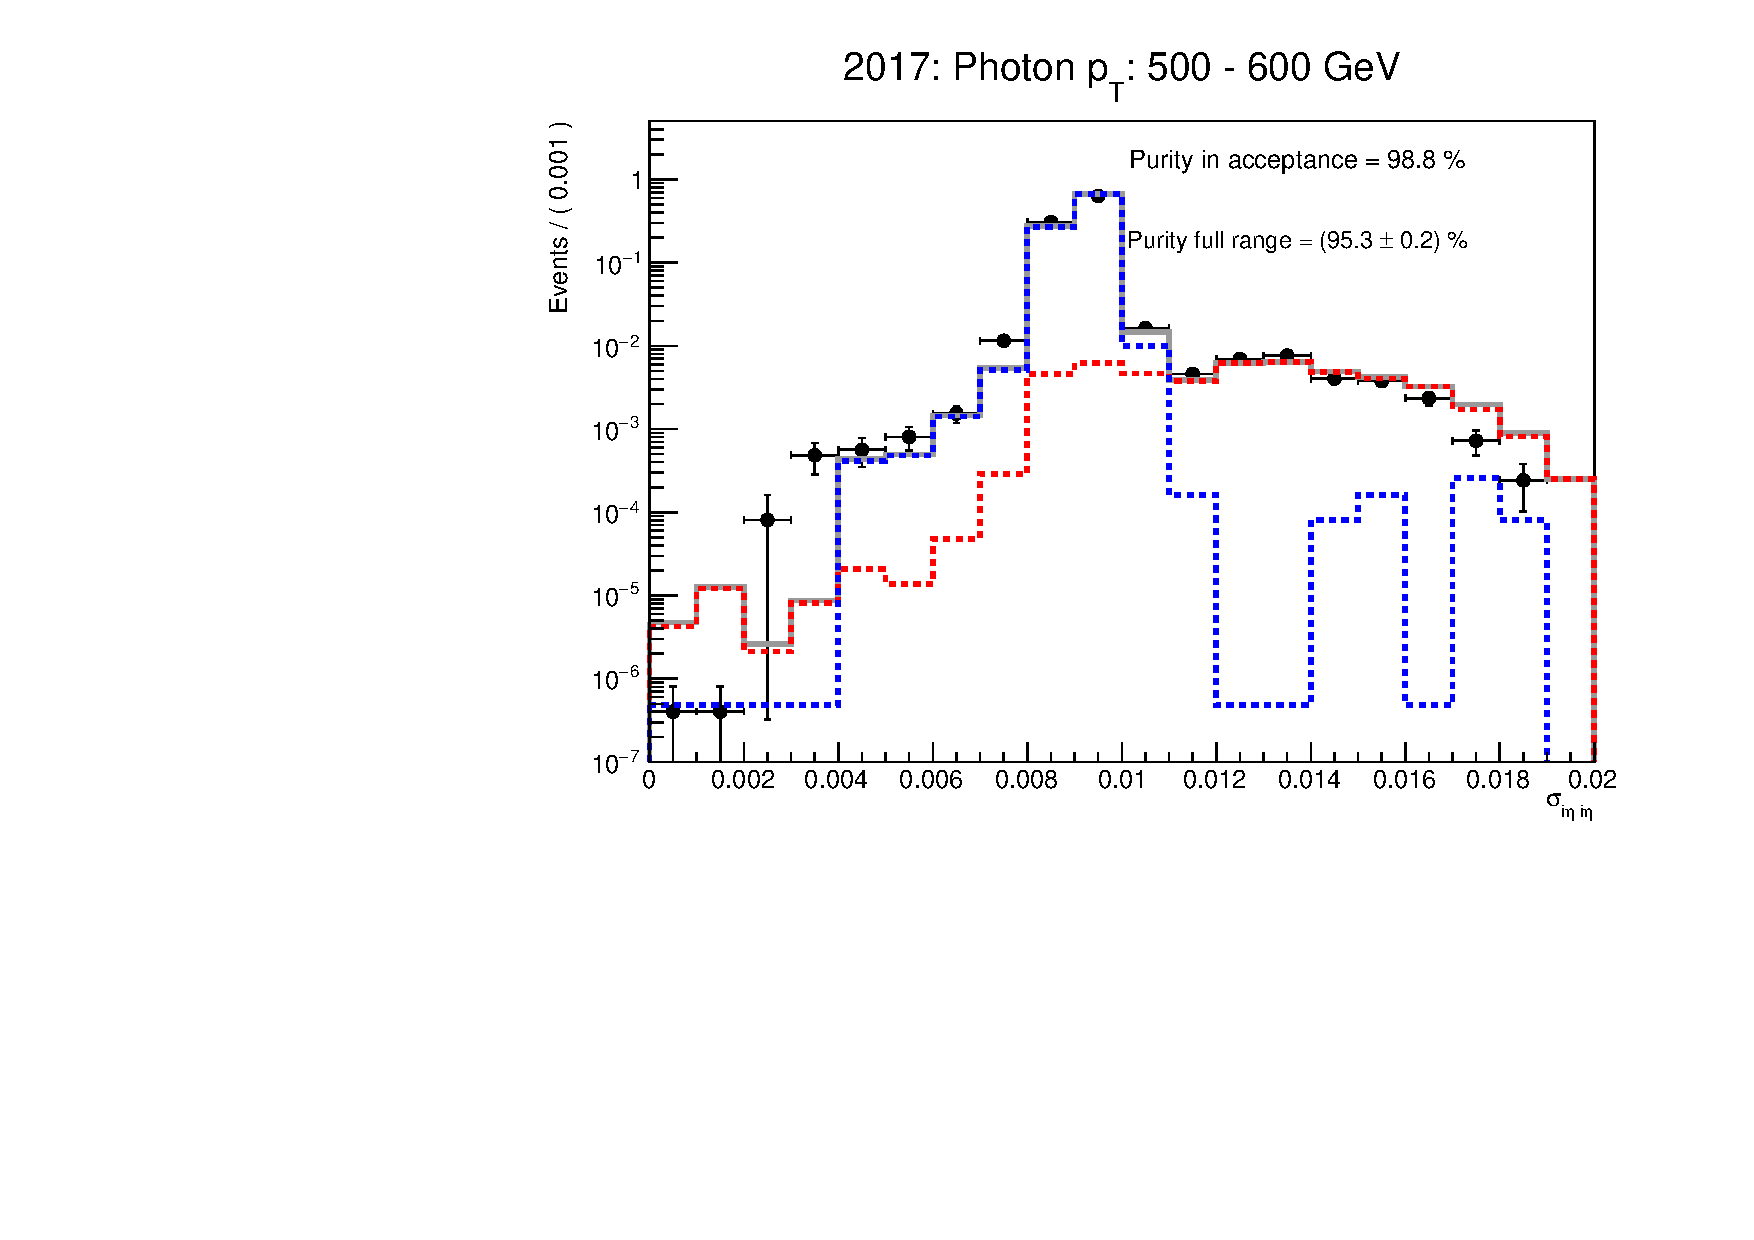
\includegraphics[width=0.45\textwidth]{PhotonPurity/fit_2017_pt500-600_nominal.pdf}
        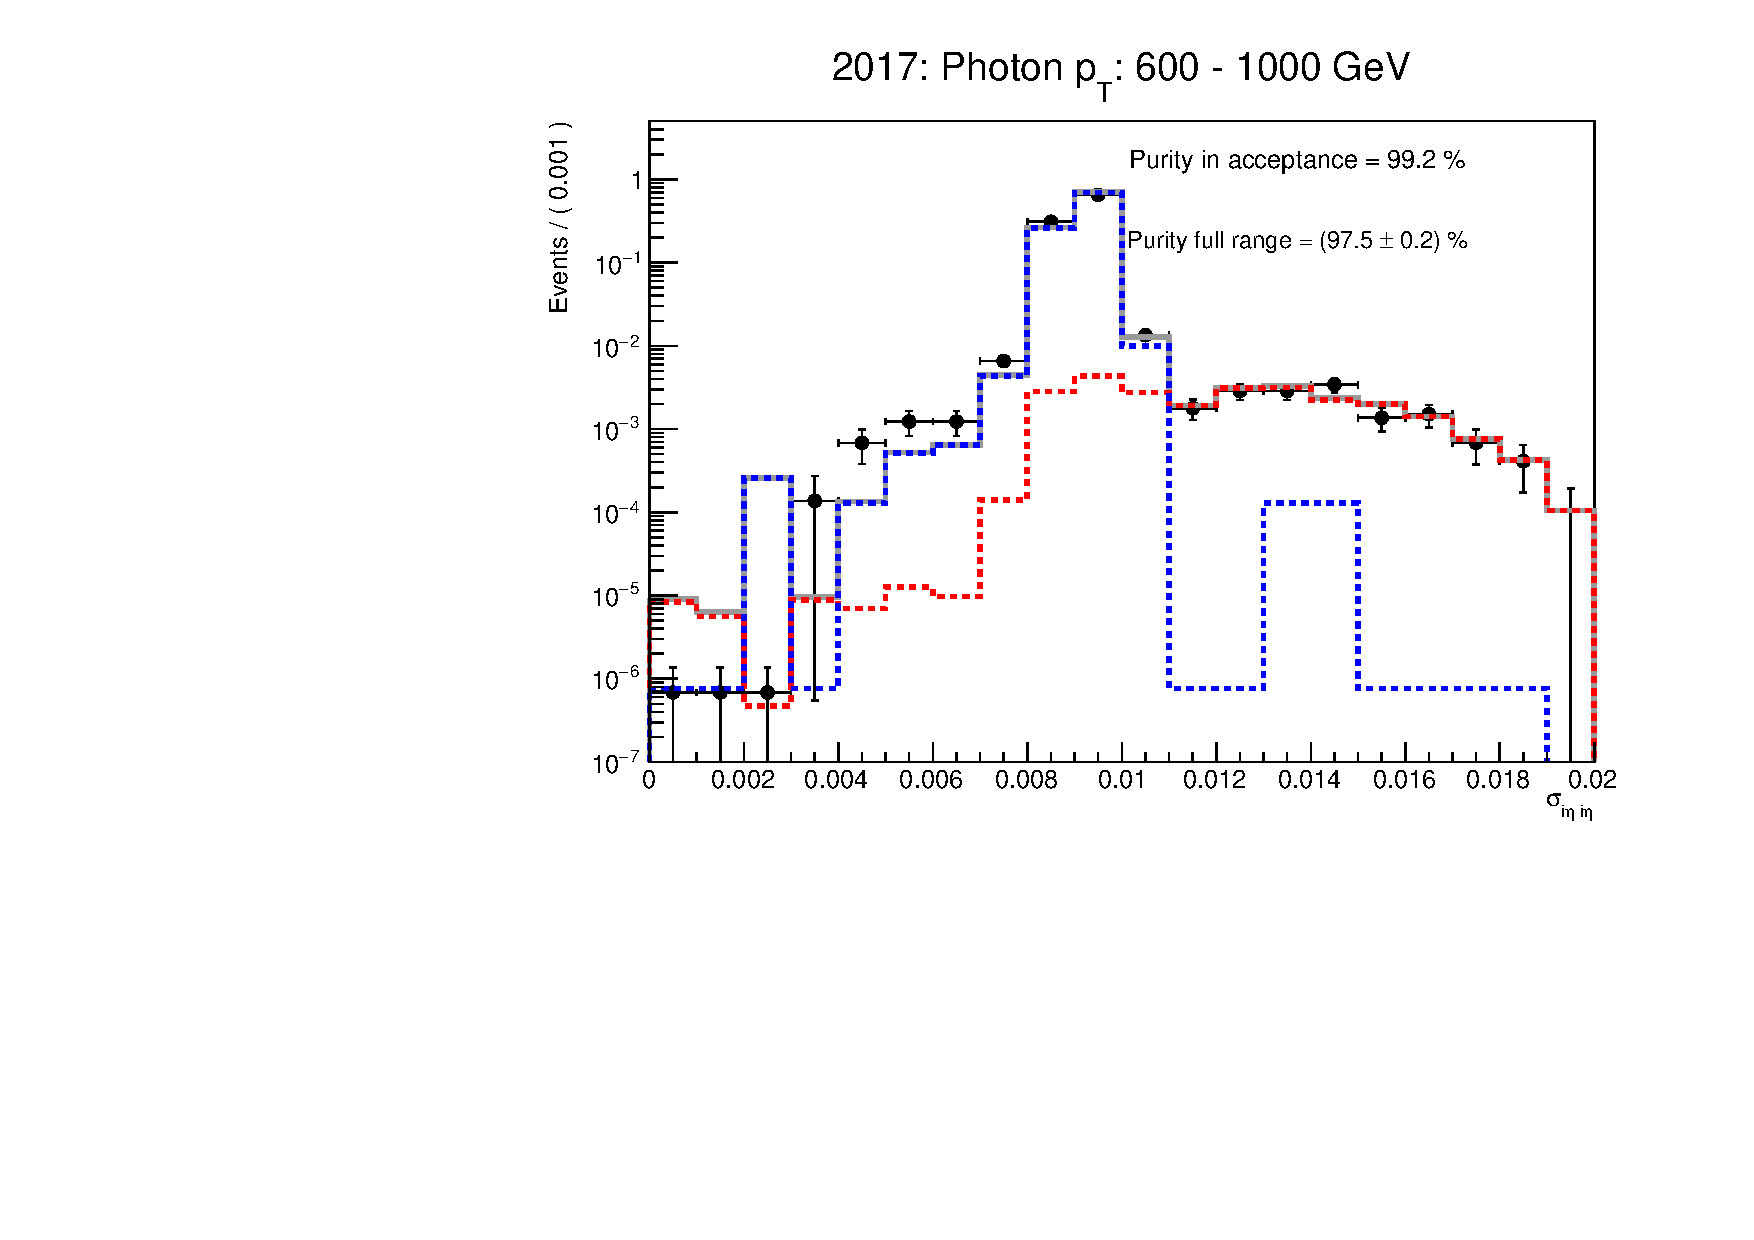
\includegraphics[width=0.45\textwidth]{PhotonPurity/fit_2017_pt600-1000_nominal.pdf}
    \caption{Template fits used to determine the photon purity in the 2017 dataset. The fits are shown in bins of photon \pt, increasing from left 
    to right and top to bottom. The ``nominal'' binning scheme is used.}
    \label{fig:purity_fits_2017}
\end{figure}

\begin{figure}[htbp]
    \centering
        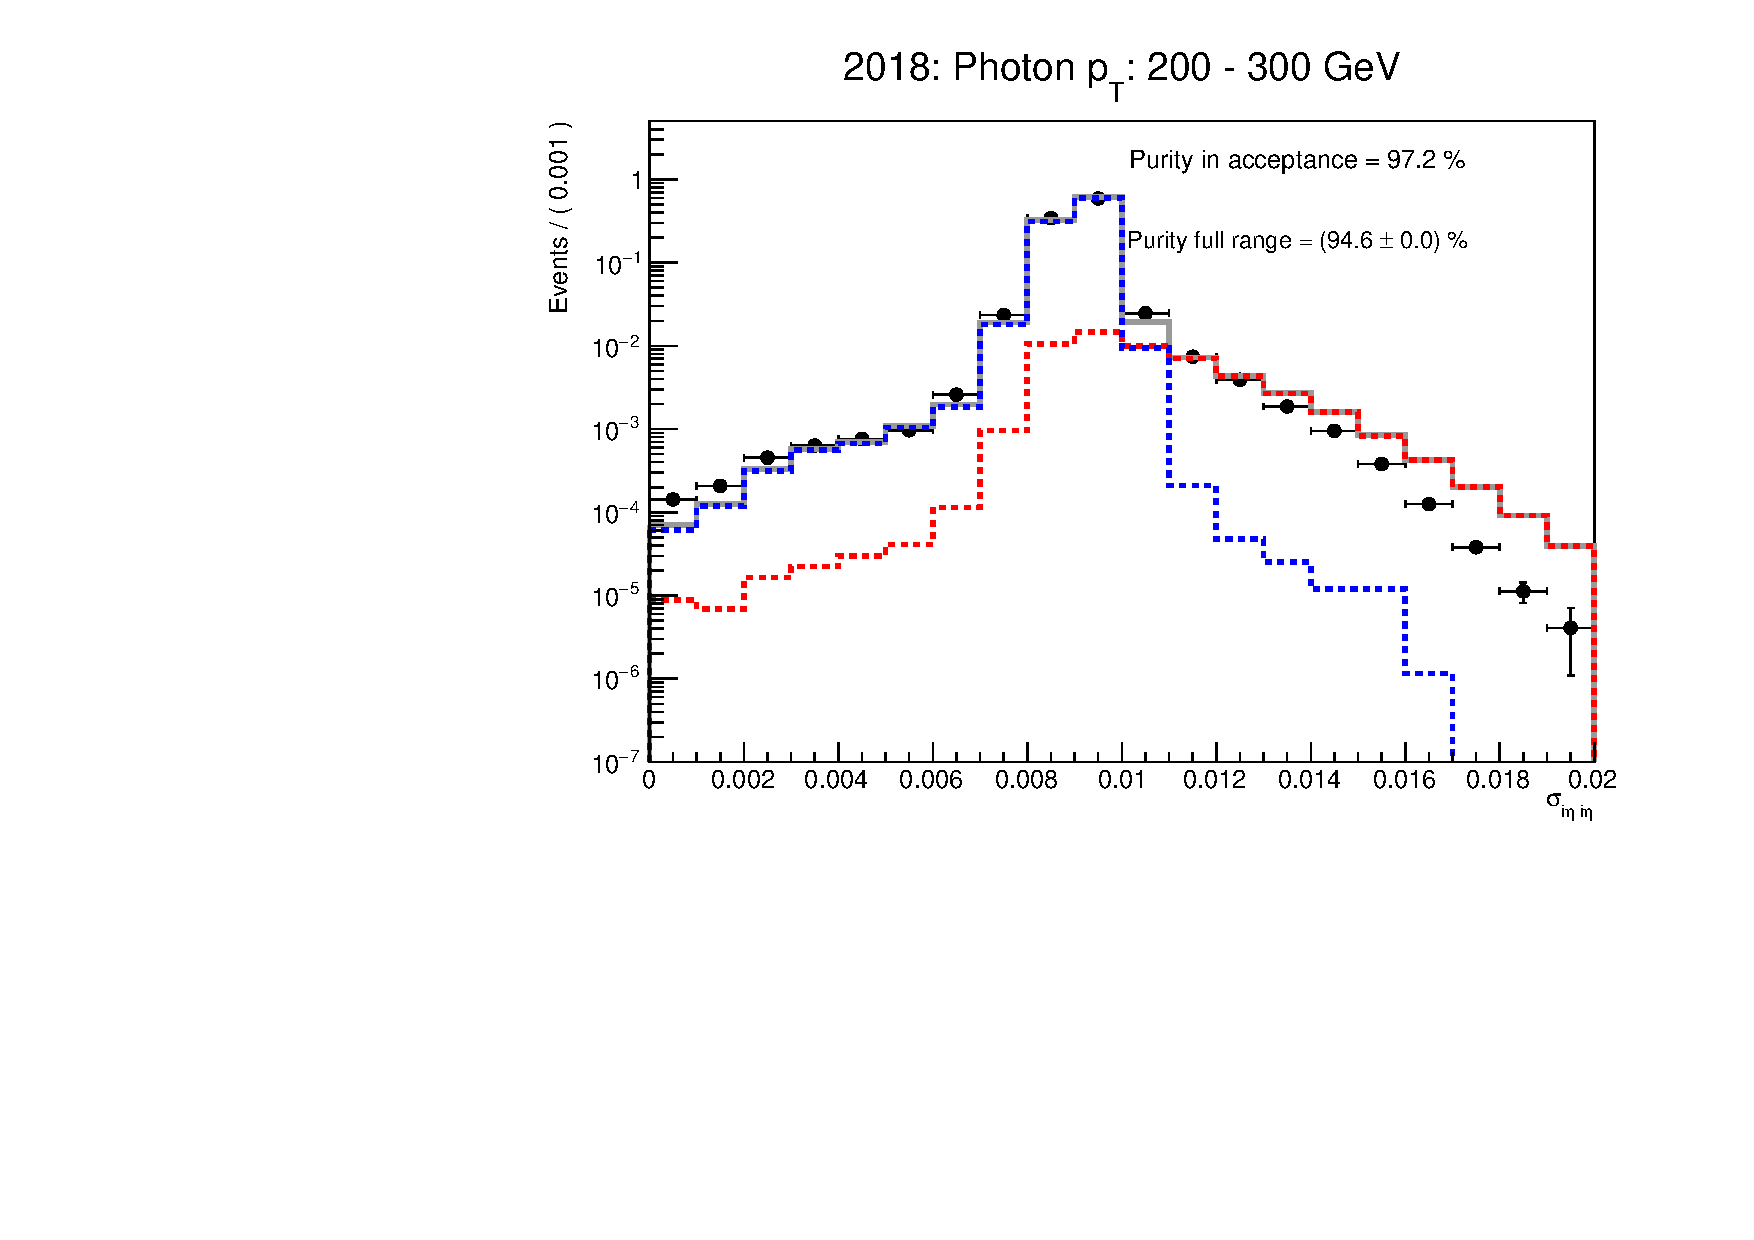
\includegraphics[width=0.45\textwidth]{PhotonPurity/fit_2018_pt200-300_nominal.pdf}
        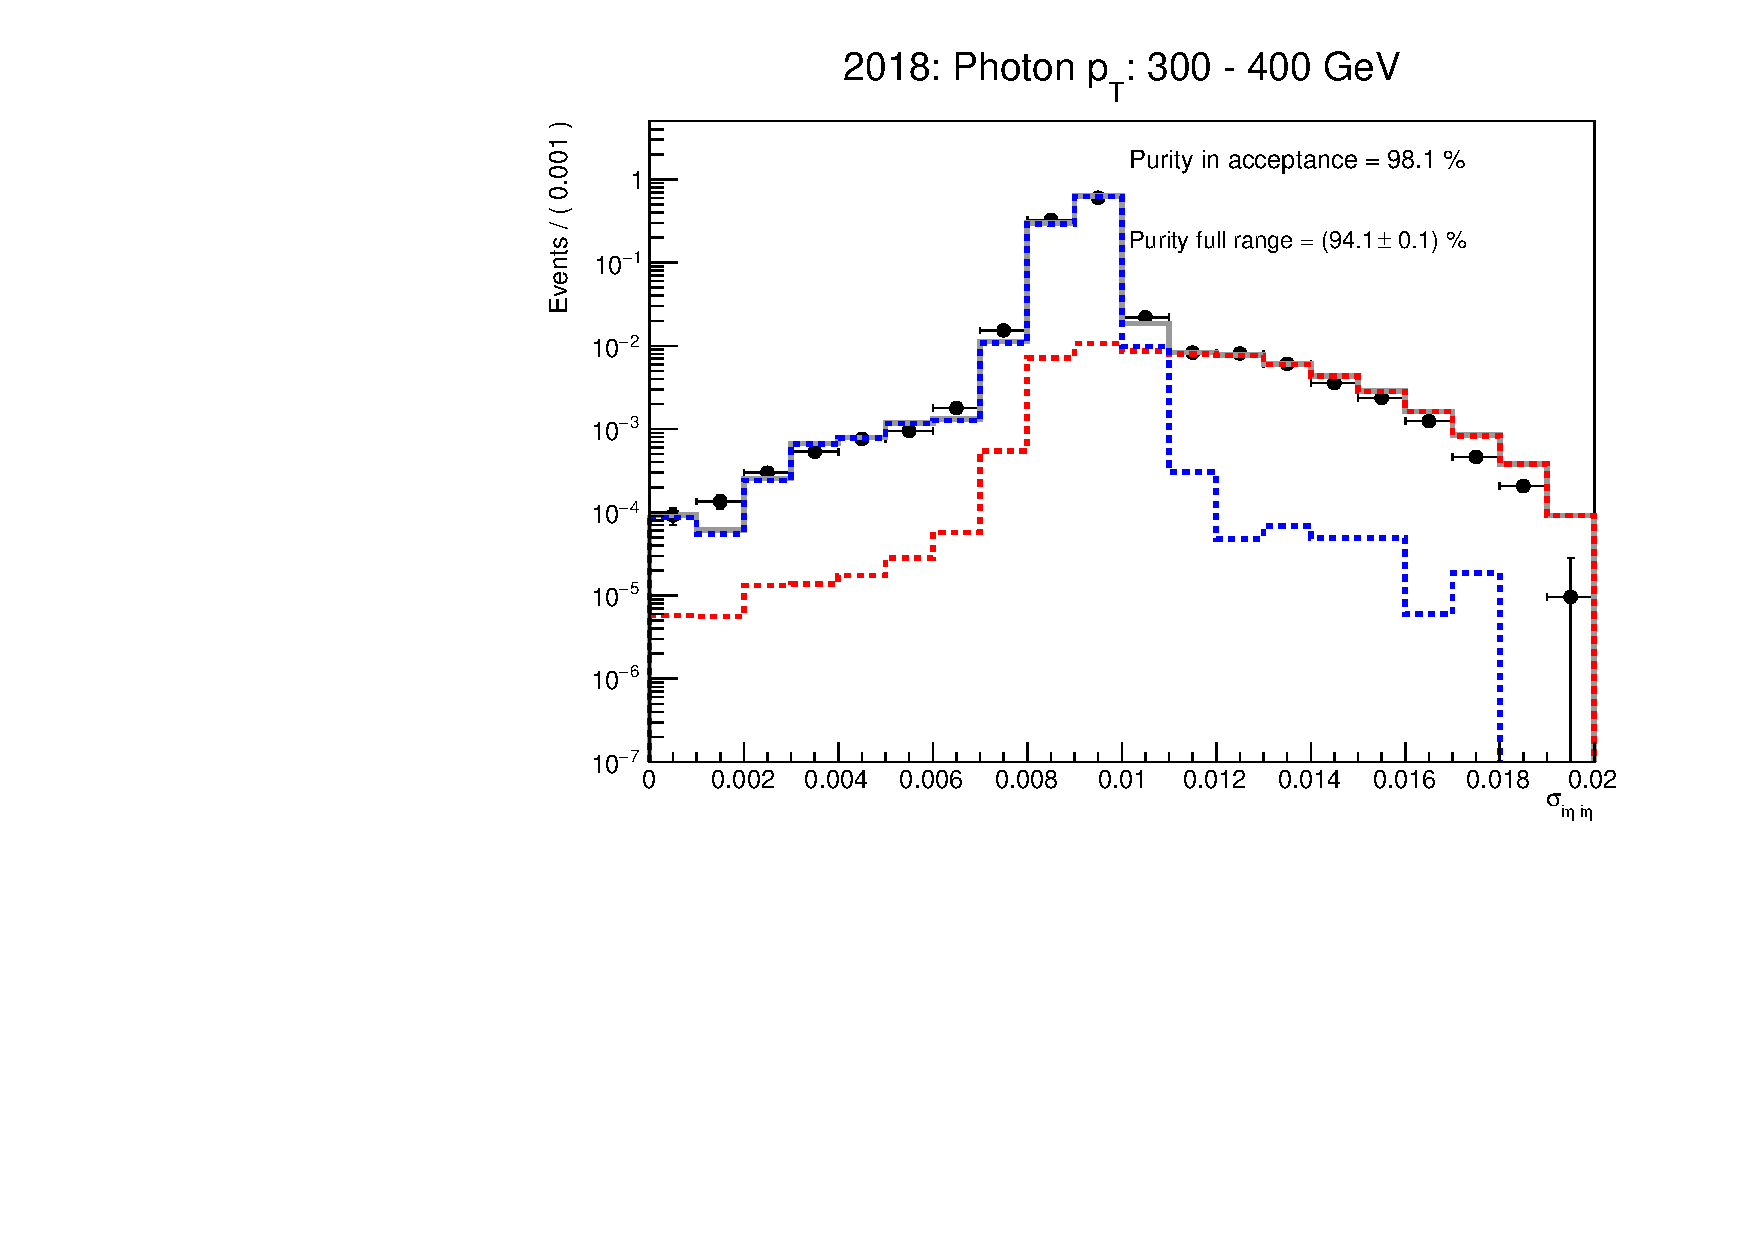
\includegraphics[width=0.45\textwidth]{PhotonPurity/fit_2018_pt300-400_nominal.pdf}
        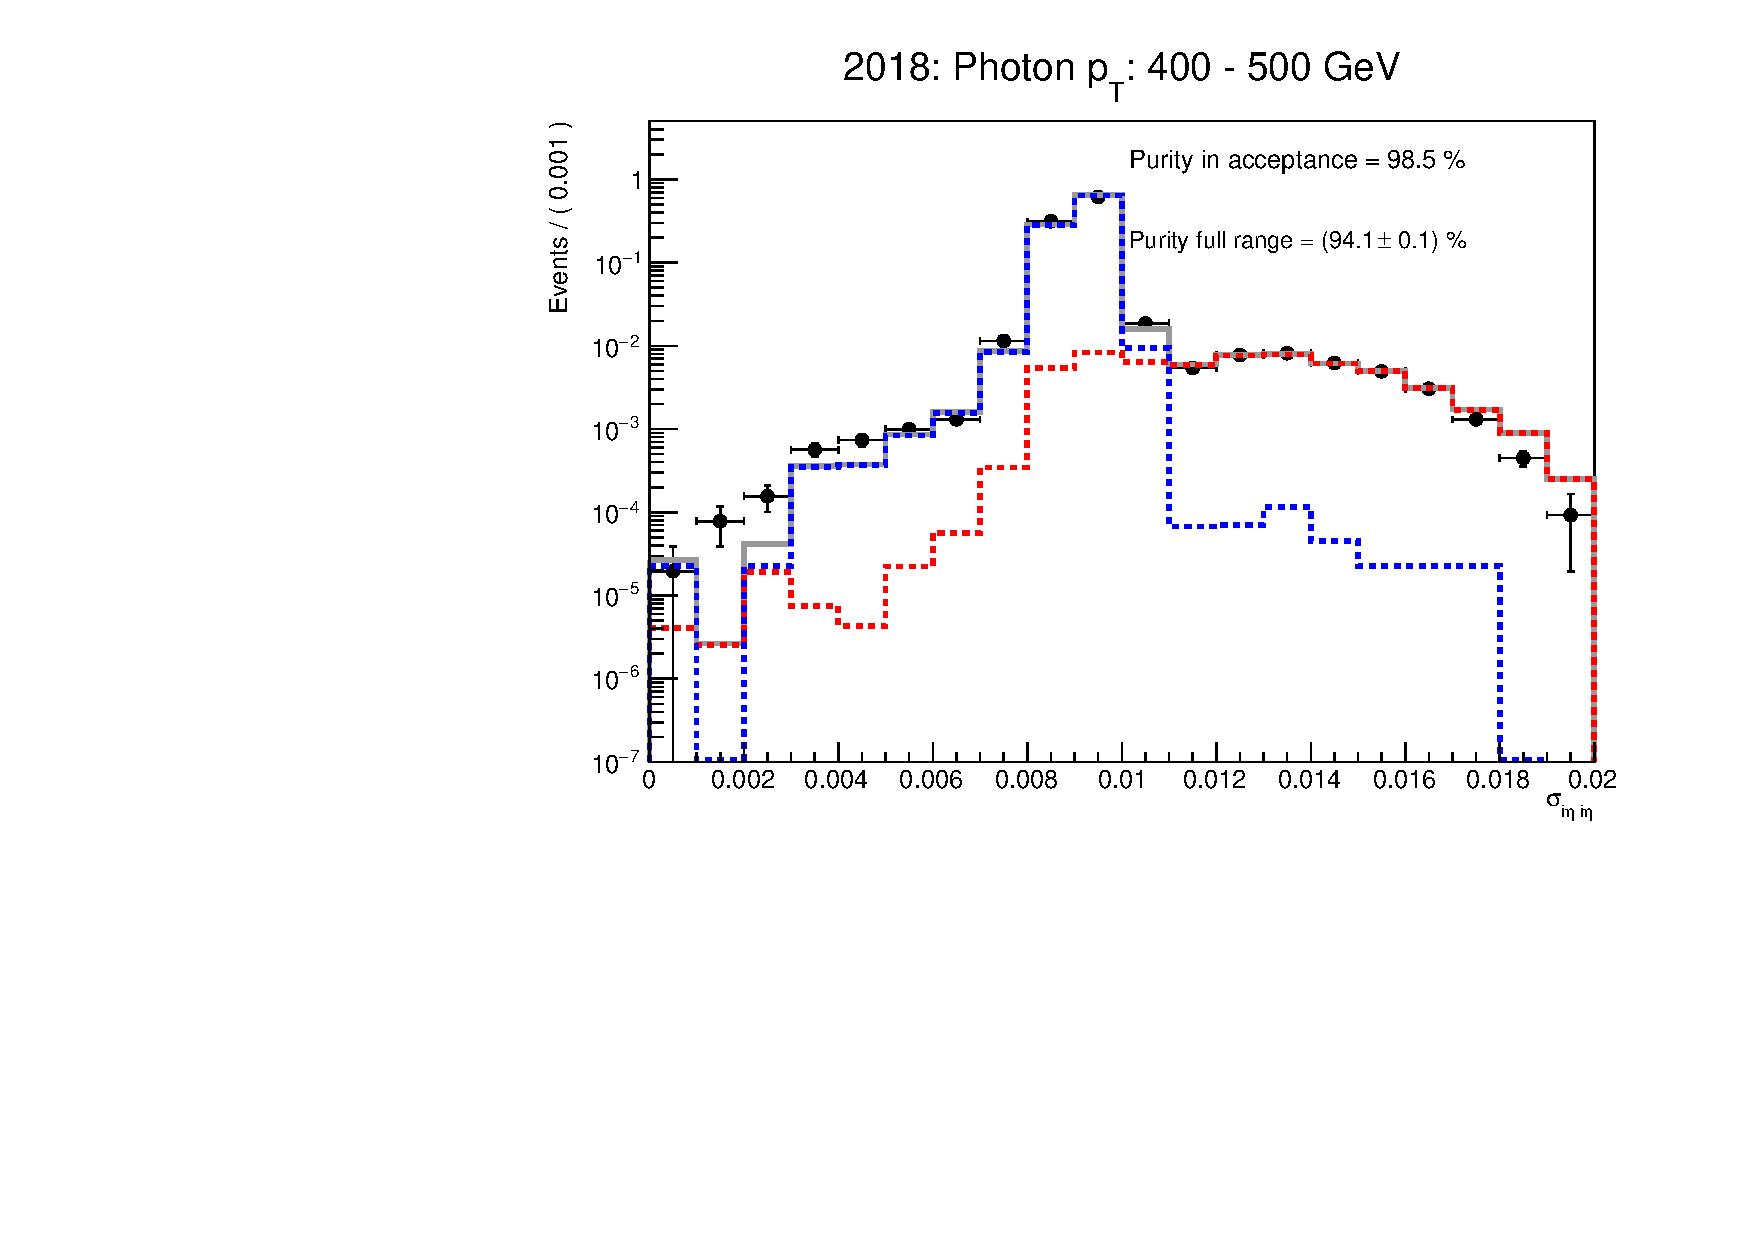
\includegraphics[width=0.45\textwidth]{PhotonPurity/fit_2018_pt400-500_nominal.pdf}
        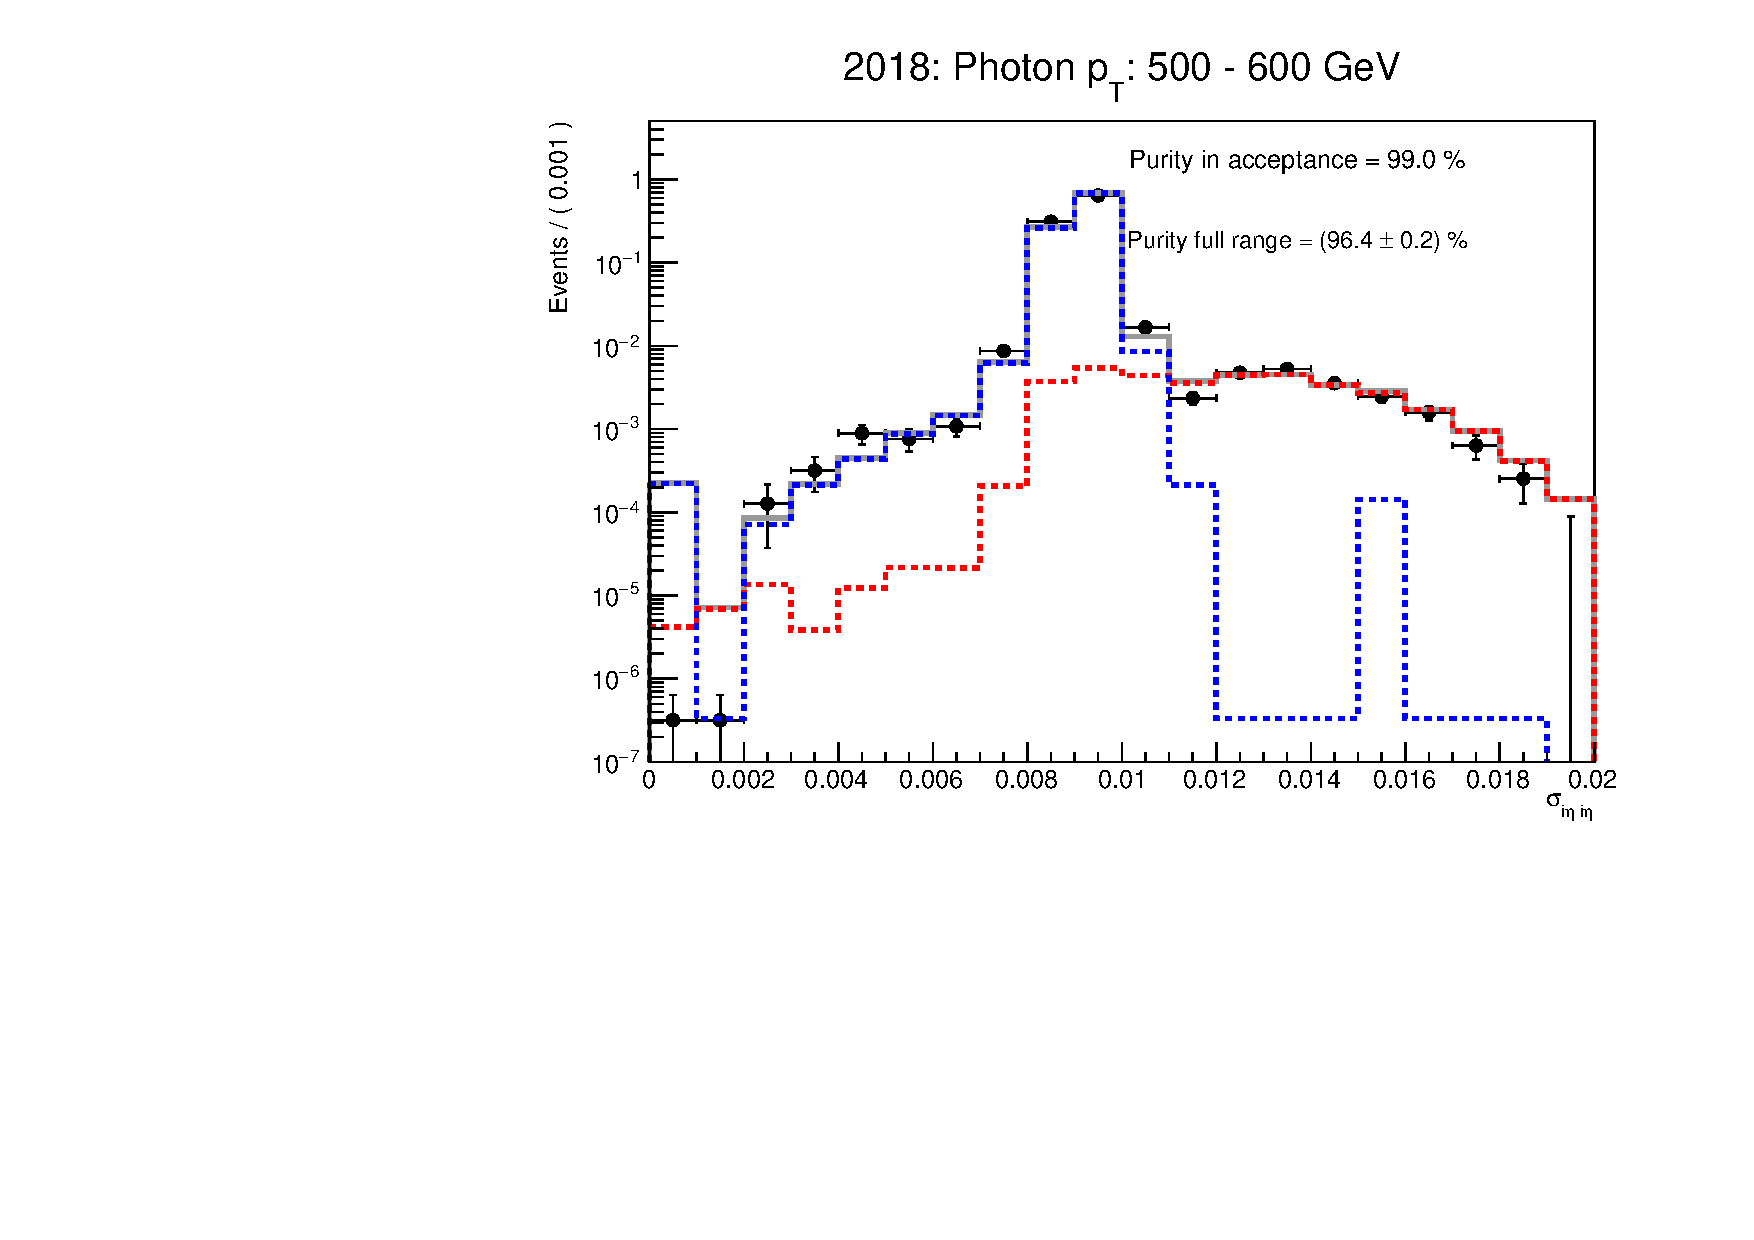
\includegraphics[width=0.45\textwidth]{PhotonPurity/fit_2018_pt500-600_nominal.pdf}
        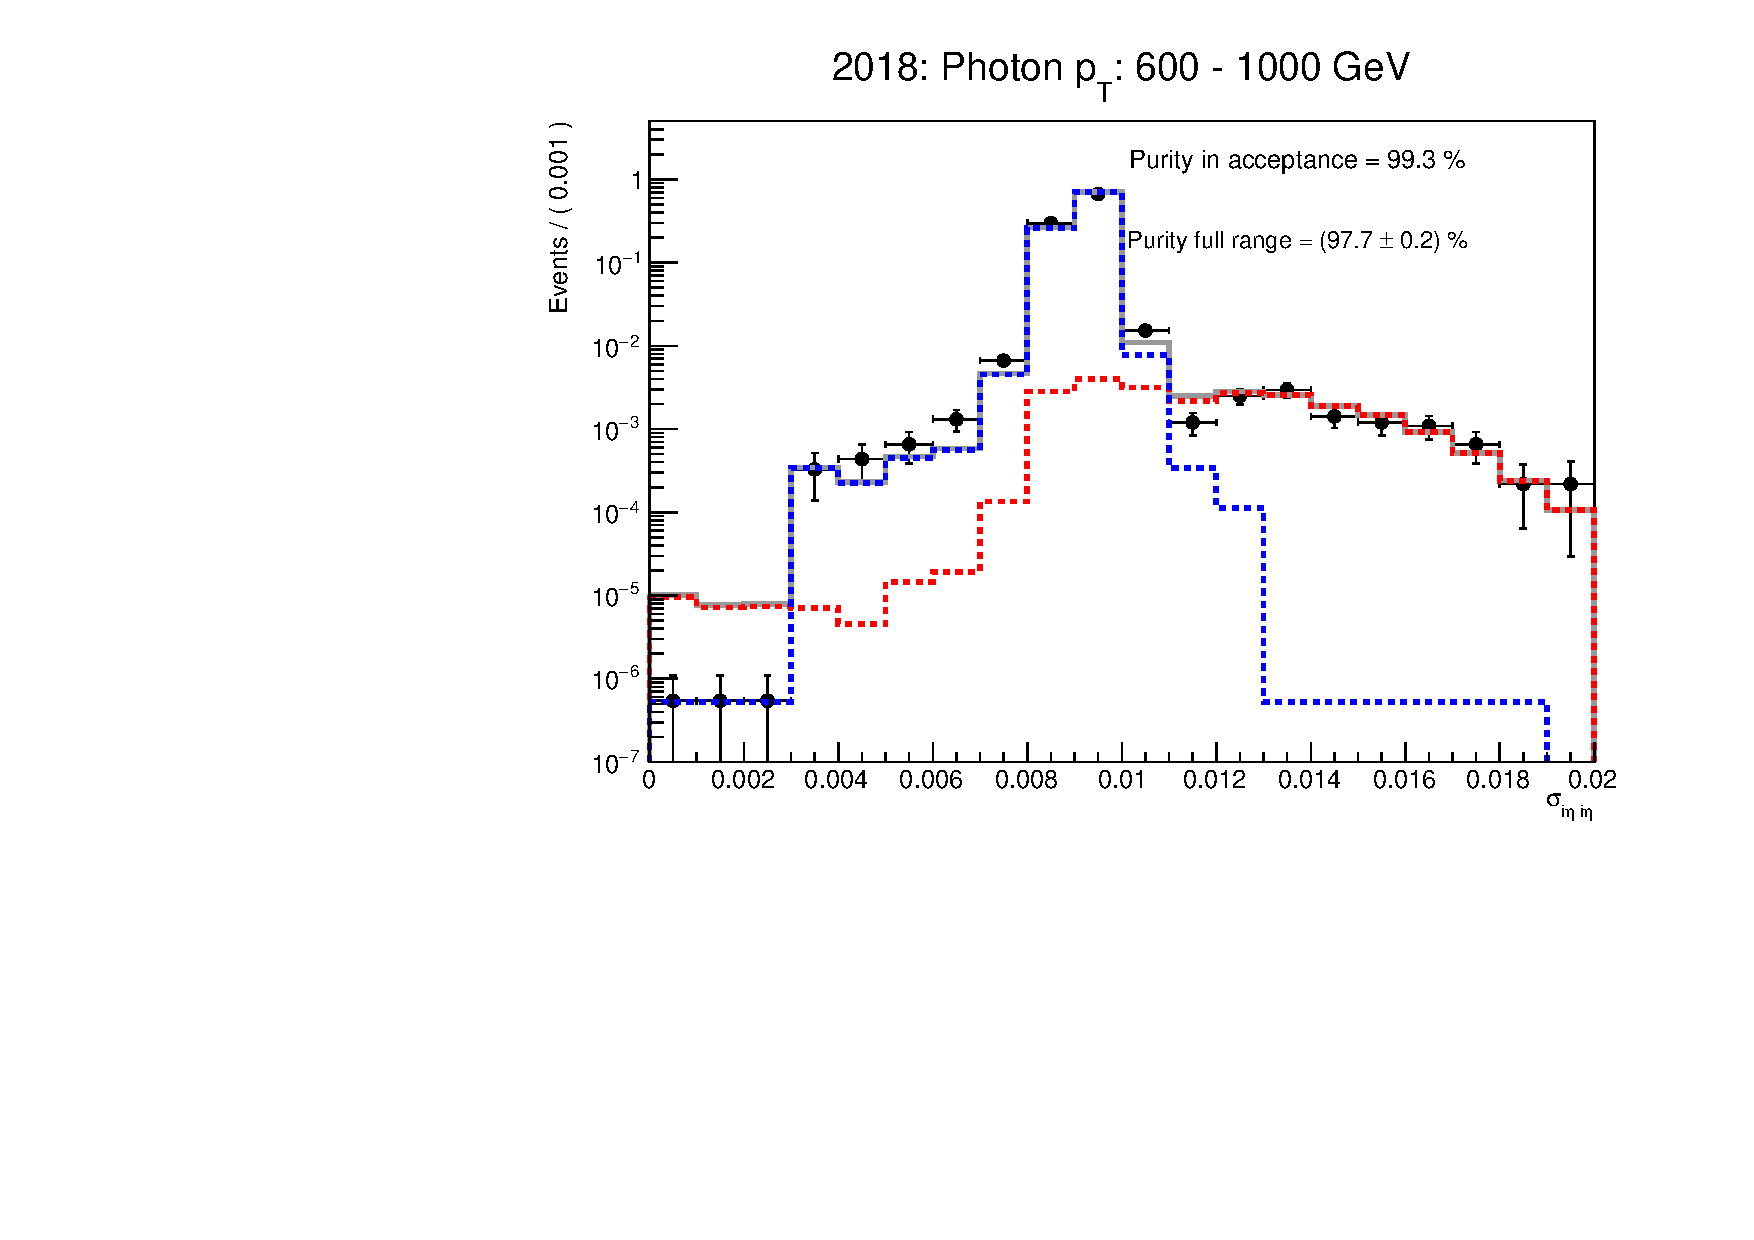
\includegraphics[width=0.45\textwidth]{PhotonPurity/fit_2018_pt600-1000_nominal.pdf}
    \caption{Template fits used to determine the photon purity in the 2018 dataset. The fits are shown in bins of photon \pt, increasing from left 
    to right and top to bottom. The ``nominal'' binning scheme is used.}
    \label{fig:purity_fits_2018}
\end{figure}

\begin{figure}[htbp]
    \centering
        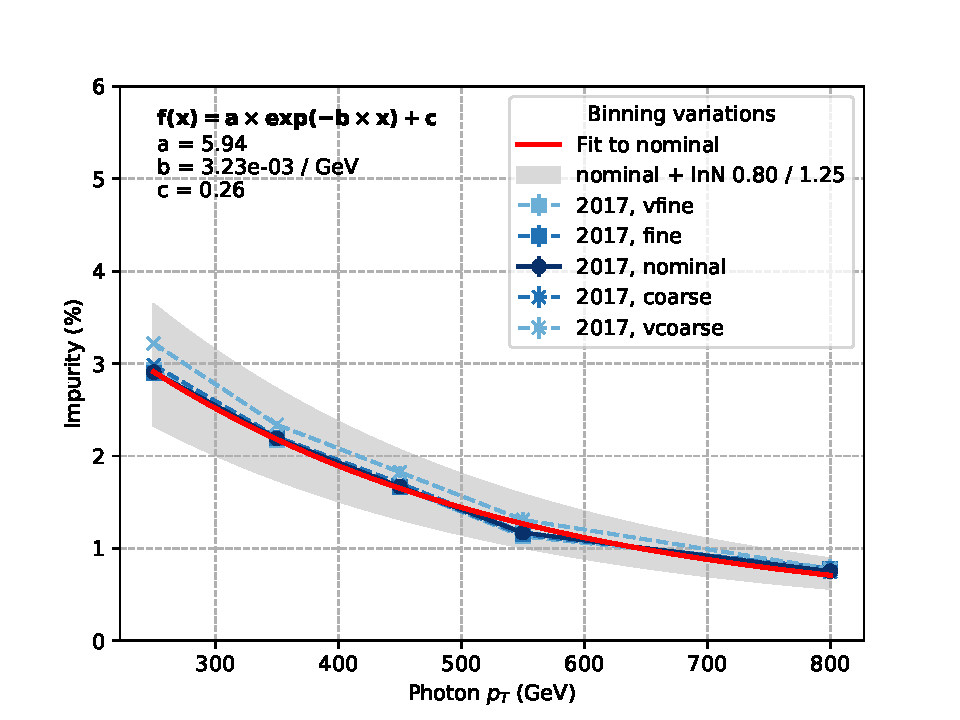
\includegraphics[width=0.48\textwidth]{PhotonPurity/purity_variations_2017.pdf}
        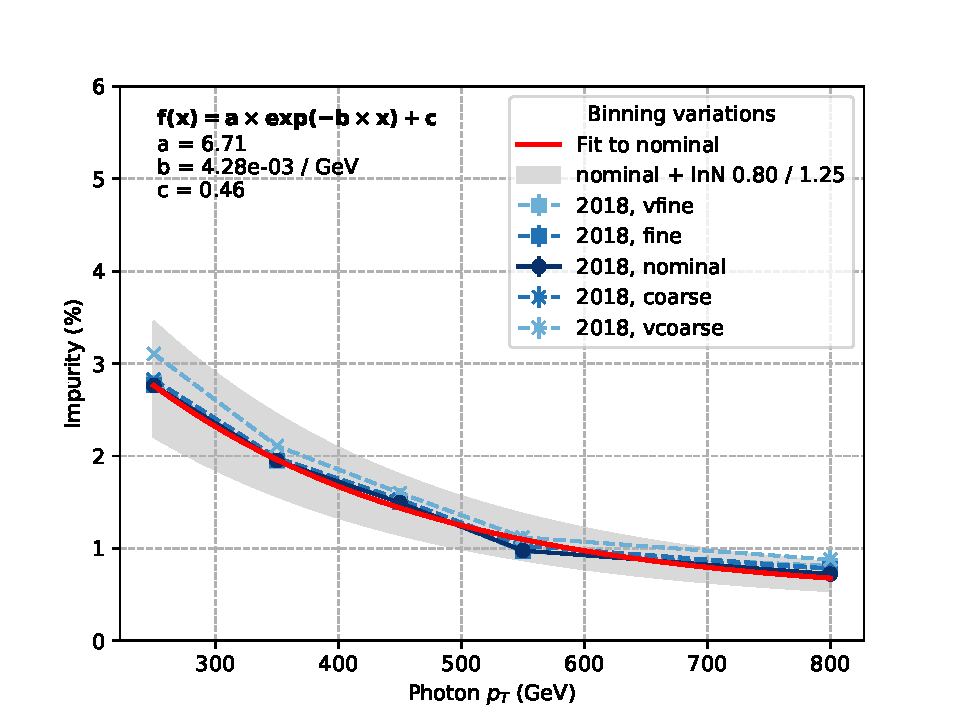
\includegraphics[width=0.48\textwidth]{PhotonPurity/purity_variations_2018.pdf}
    \caption{Photon impurity as a function of photon \pt for 2017 (left) and 2018 (right). The measured values for different binning choices 
    are shown in the blue shaded lines and markers. The nominal result is interpolated using an exponential function fit, which is shown in 
    the red solid line. The gray band represents a 25\% uncertainty around the interpolated nominal result.}
    \label{fig:purity_result}
\end{figure}

\begin{figure}[htbp]
    \centering
        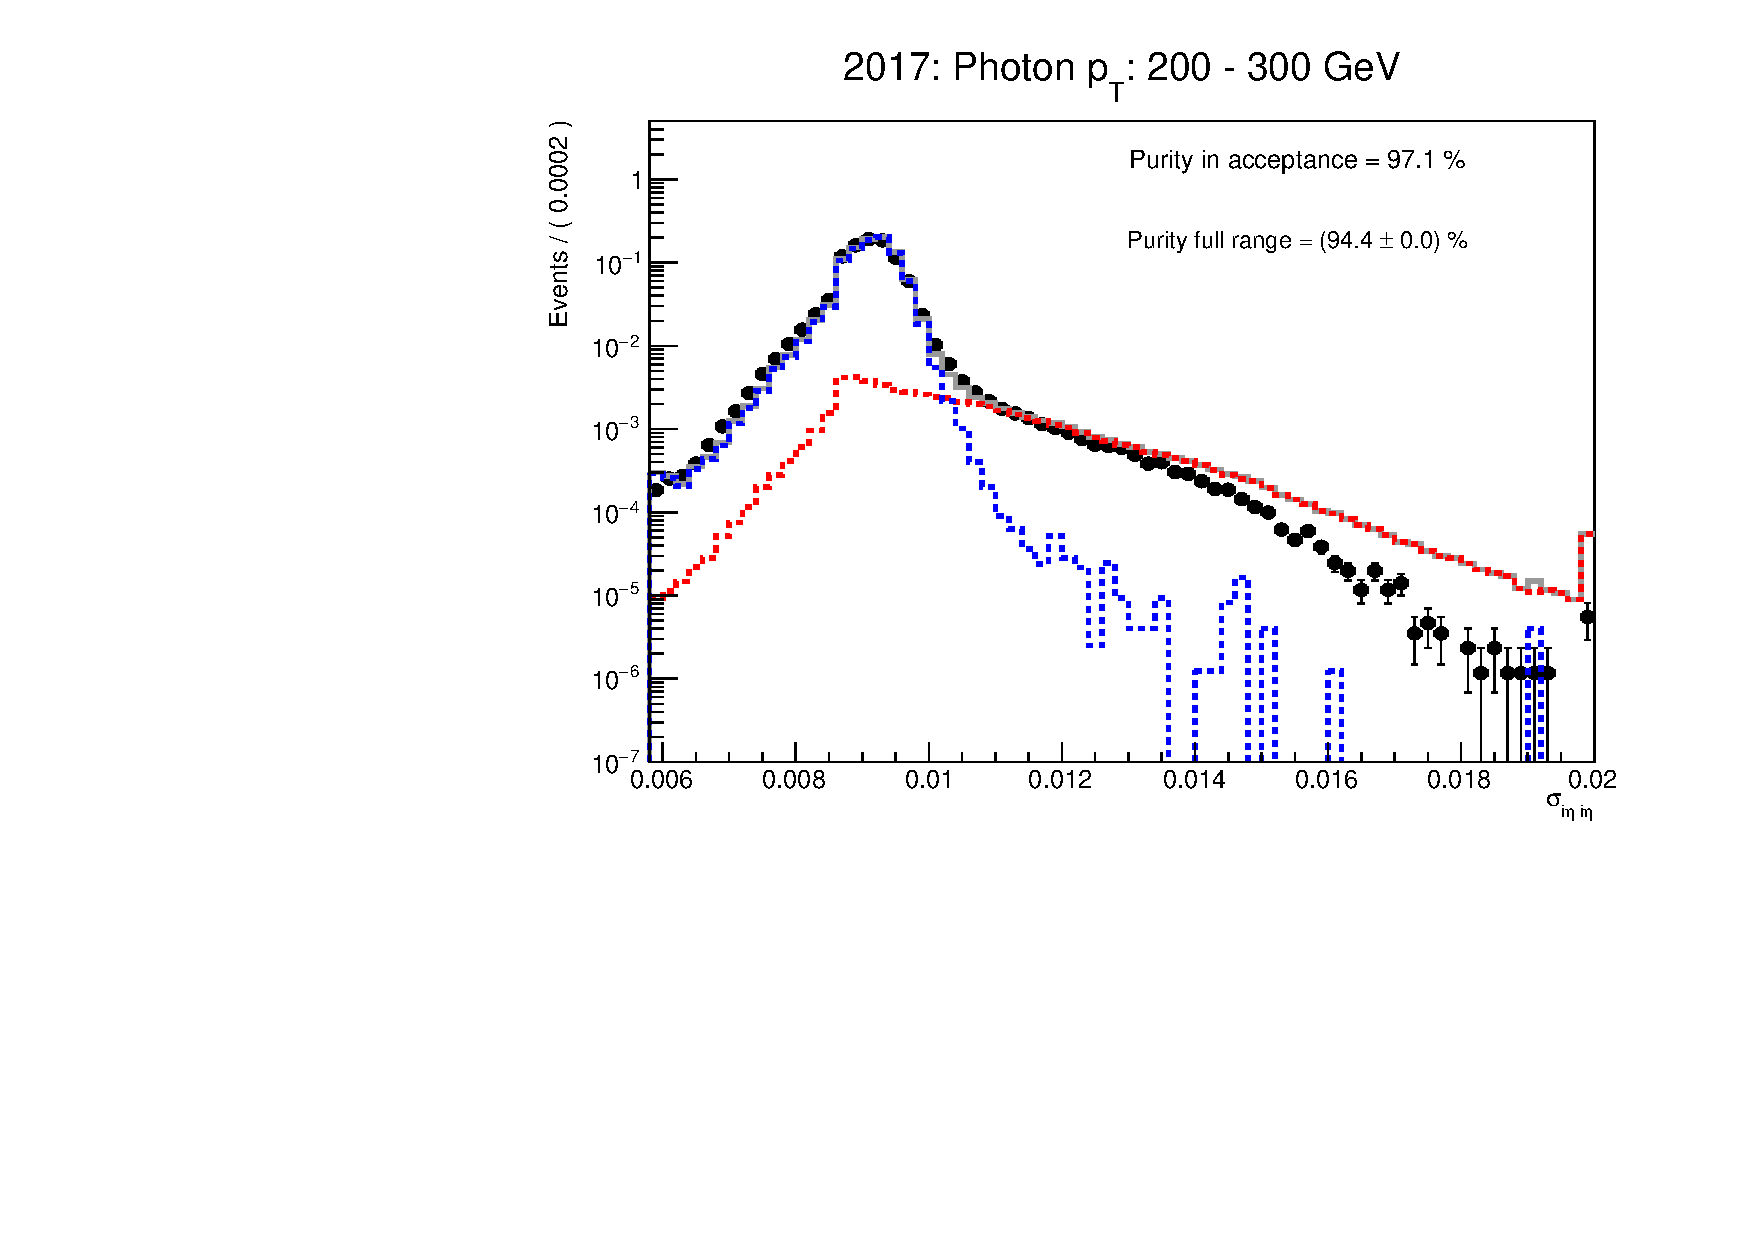
\includegraphics[width=0.45\textwidth]{PhotonPurity/fit_2017_pt200-300_vfine.pdf}
        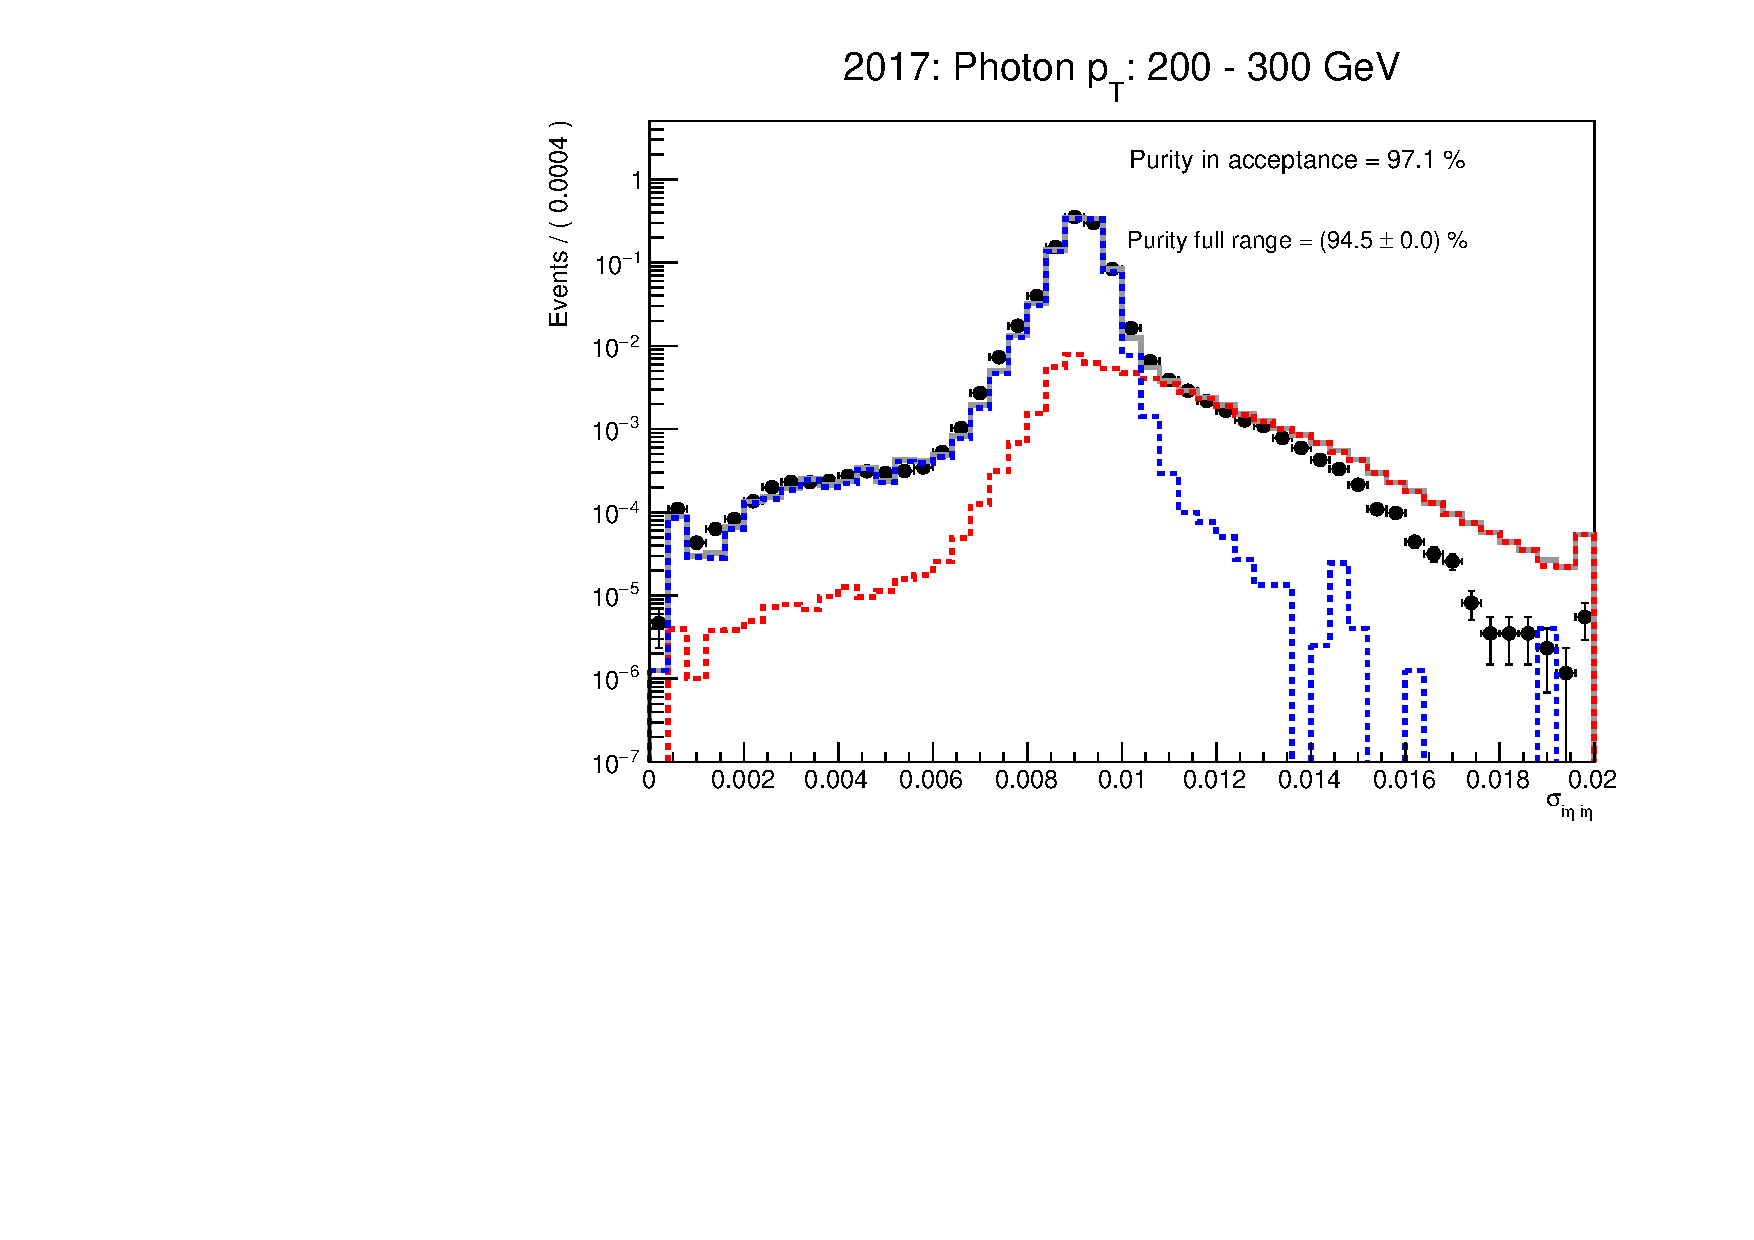
\includegraphics[width=0.45\textwidth]{PhotonPurity/fit_2017_pt200-300_fine.pdf} \\
        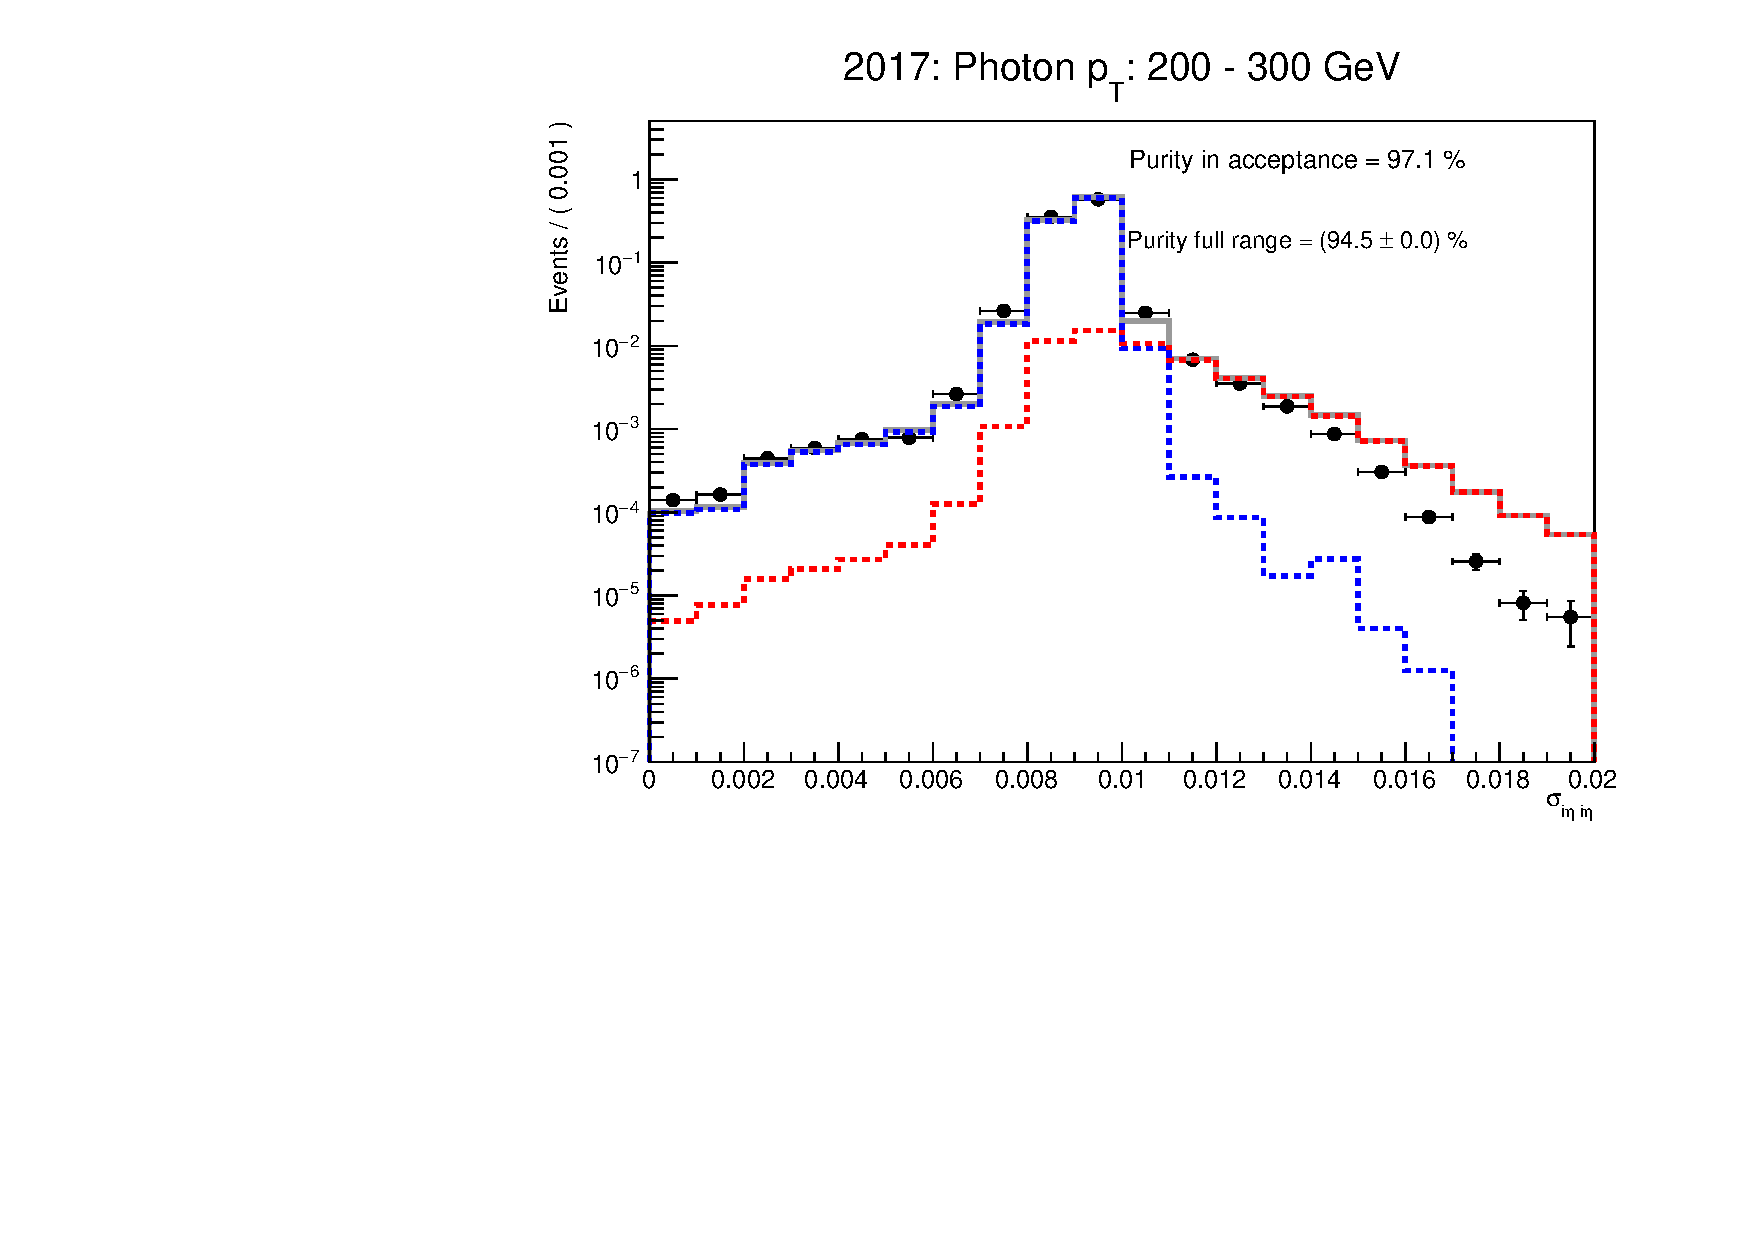
\includegraphics[width=0.45\textwidth]{PhotonPurity/fit_2017_pt200-300_nominal.pdf} \\
        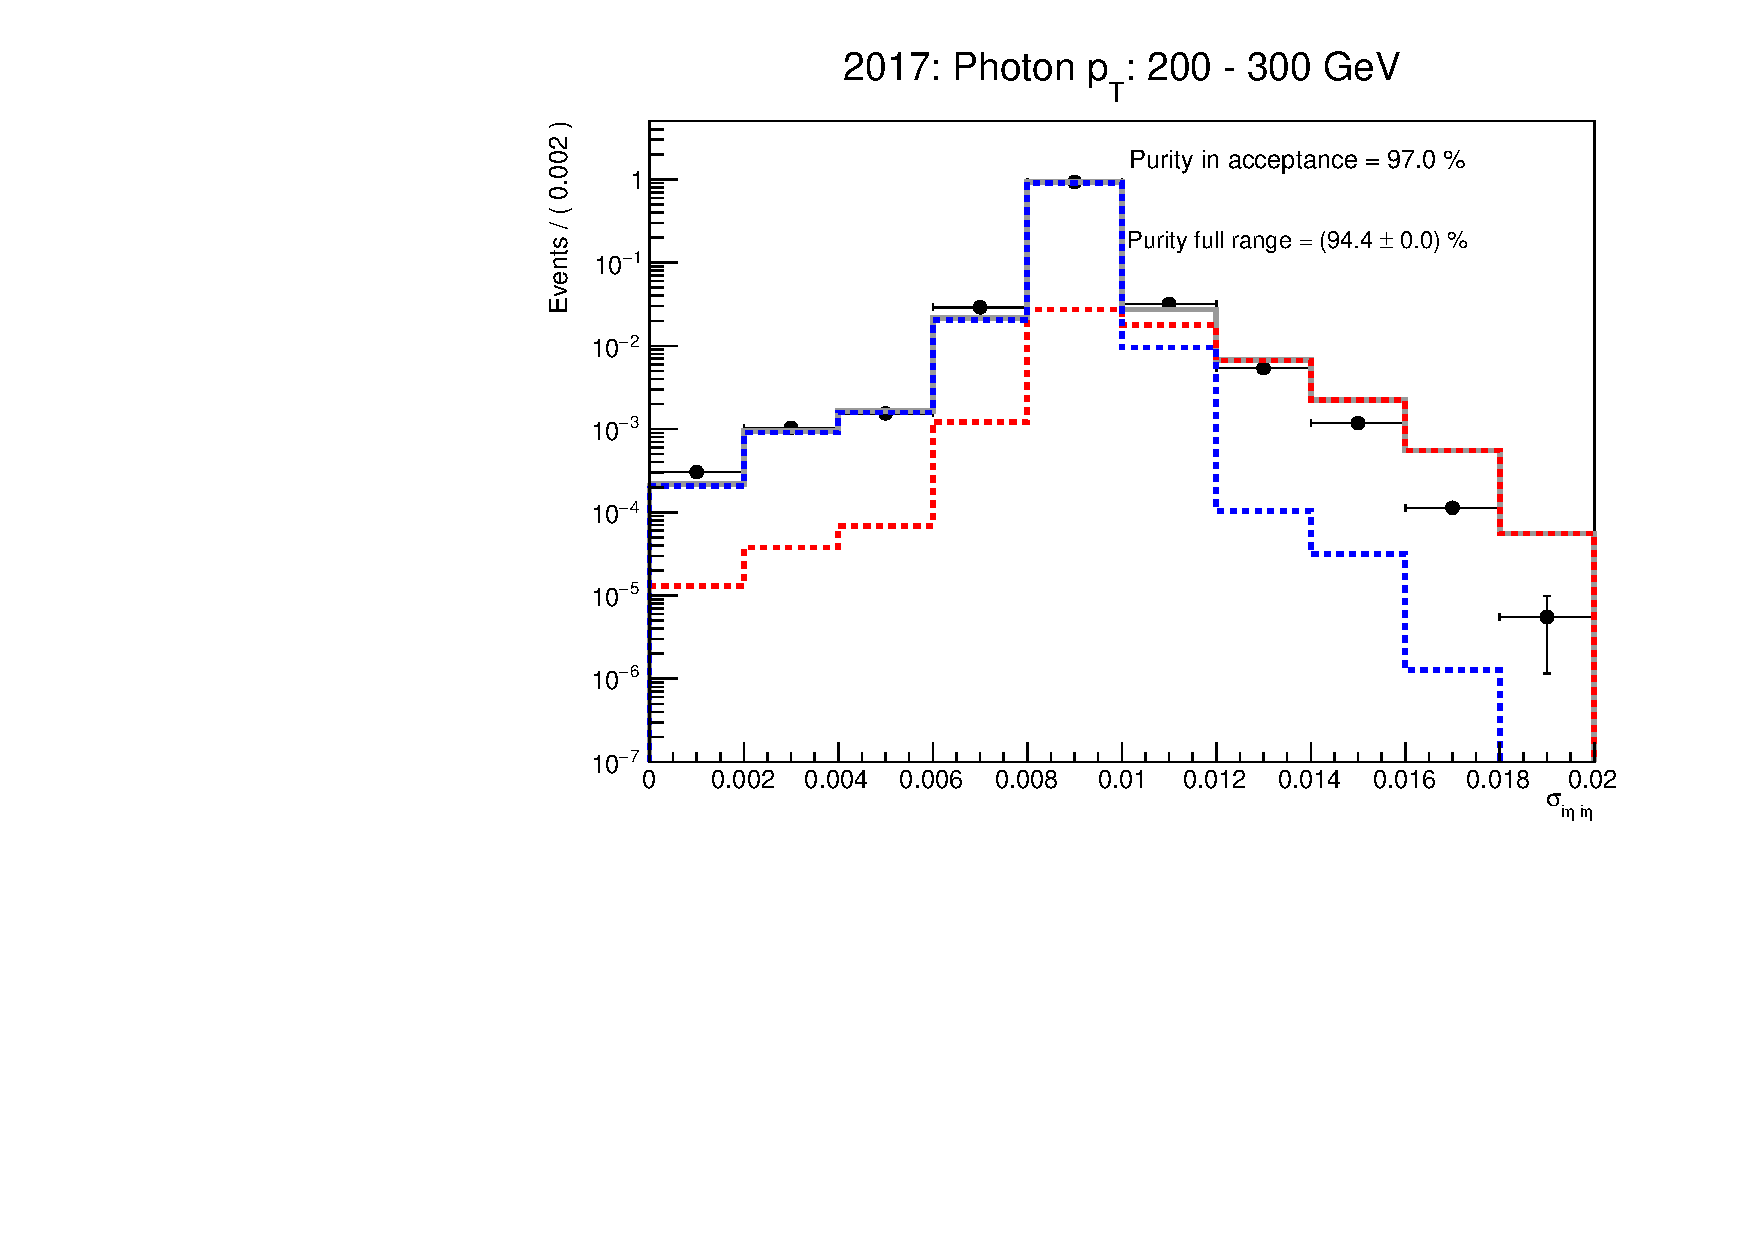
\includegraphics[width=0.45\textwidth]{PhotonPurity/fit_2017_pt200-300_coarse.pdf}
        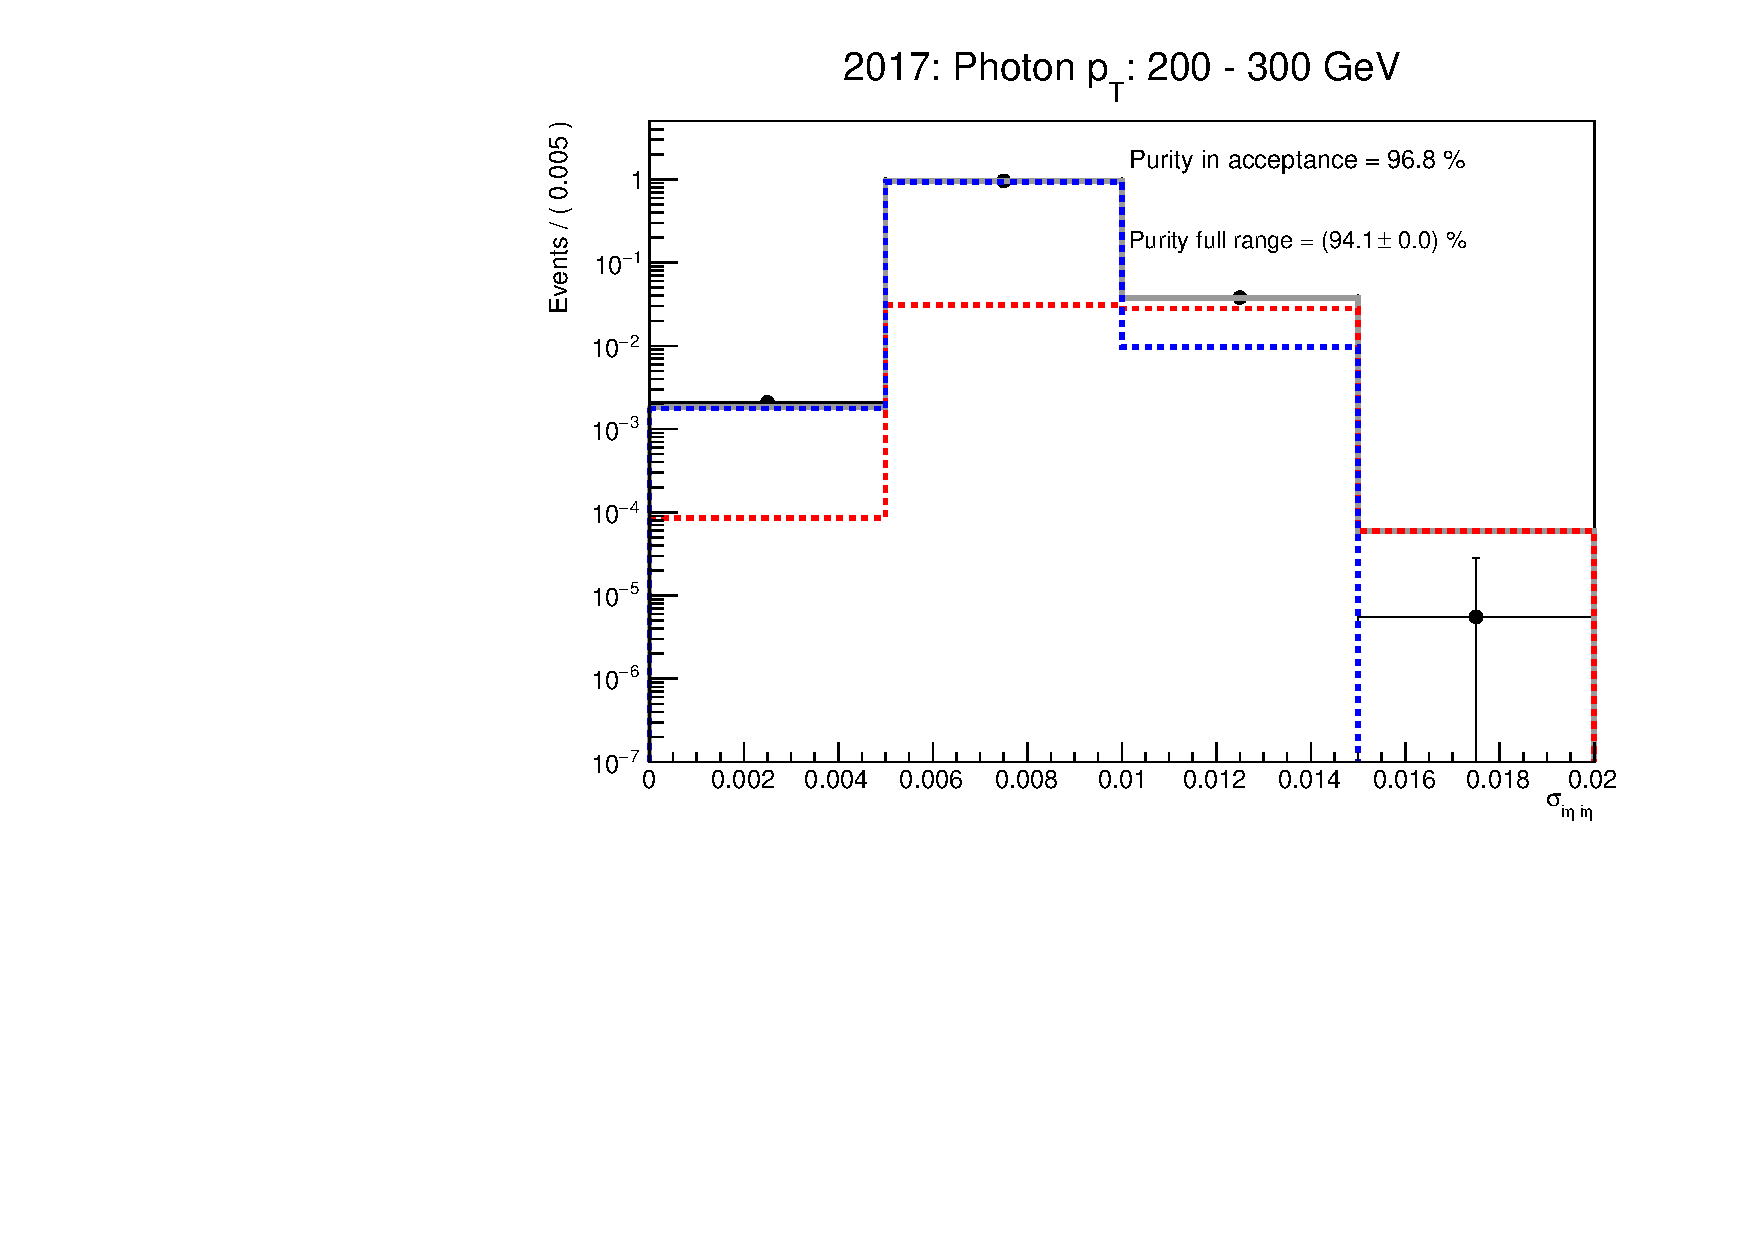
\includegraphics[width=0.45\textwidth]{PhotonPurity/fit_2017_pt200-300_vcoarse.pdf}
    \caption{Comparison of binning schemes used to define a systematic uncertainty on the purity measurement. In all cases, the 
    $200<\pt<300$ GeV bin of the 2017 data set is shown. The binning choices are very fine and fine (top row), nominal (middle row), 
    and coarse and very coarse (bottom row).}
    \label{fig:purity_binning}
\end{figure}

\clearpage
\section{Reweighting of simulated events} \label{sec:reweighting}

\graphicspath{{3_DataAnalysisStrategy/Figures}}

Simulated signal and background samples can differ from collision data due to
various effects. Therefore, reweighting of simulated events is necessary to correct
simulated samples for these effects. The reweighting procedure for different types of 
effects are outlined in this section.

\subsection{Trigger efficiency reweighting}
\label{subsec:trigger_eff_reweighting}

\subsubsection{\ptmissnomu and \htmissnomu triggers}
\label{subsubsec:met_trigger_eff}

In this analysis, the collision data for signal region, $W(\mu \nu)$ and $Z(\mu \mu)$ 
control regions (see Sec.~\ref{sec:event_selection}) are collected using high-level triggers 
that require $\ptmissnomu > 120$ GeV
and $\htmissnomu > 120$ GeV. The fact that muon momenta are subtracted
from the $\ptmiss$ and $\htmiss$ calculations allow these triggers to be used both for collecting data in
signal region (high $\ptmiss$), and muon control regions (high \pt muons).
To simplify the discussion, this trigger will be referred to as the ``MET trigger'' in this text.

The efficiency of MET trigger is calculated using $\Wmnjets$ events, as a function of recoil.
Here, recoil refers to the vectorial sum of the missing transverse momentum (MET) and the muon transverse momentum,
as defined in Eq.~\ref{eq:recoil_def}. The $\Wmnjets$ events are selected by requiring 
the event to pass \texttt{HLT\_IsoMu27} trigger for 2017, and \texttt{HLT\_IsoMu24} 
for 2018. In addition, the reconstructed muon is required to be tightly-identified as defined in Sec.~\ref{subsec:muons}, 
and have $\pt > 40$ GeV. The full set of selections is listed below:

\begin{enumerate}
  \item Event must have exactly one tightly-identified muon with $\pt > 40$ GeV.
  \item Veto on additional leptons, photons, b jets, $\tau_{had}$ candidates.
  \item $\Delta\phi(jet,\ptvecmiss)>0.5$ for the four leading jets with $\pt>30$ GeV.
  \item (Calo \ptmiss - PF \ptmiss) / recoil $<$ 0.5
  \item Leading AK4 jet with $\pt>80$ GeV, passing the tight jet ID.
  \item Subleading AK4 jet with $\pt>40$ GeV.
  \item $\detajj > 1.0$
  \item $\dphijj < 1.5$
\end{enumerate}

The efficiency of the MET trigger is computed separately for data and Monte Carlo simulation (MC),
and the ratio between those two measurements are used to derive scale factors (SF) to correct the MC.
The efficiency measurement procedure is described below.

To understand the dependence of the efficiencies on the jet kinematics, the efficiencies in data and MC are measured 
separately for two cases: Events where the two highest-$\pt$ jets are both in the central region of the detector (i.e. $|\eta| < 2.5$), 
and events where at least one jet is in the forward region ($|\eta| > 2.5$).

To smooth out the fluctuations in efficiencies for each case, a sigmoid function is fit to both data and MC 
efficiency curves. The sigmoid function has three parameters and is written in the form $f(x,a,b,c) = \frac{c}{1+e^{-a(x-b)}}$. 
The factors for correcting the MC simulation are then calculated as the ratio of the best-fit sigmoid curves for data and MC.
The efficiencies and resulting SFs are shown in Fig.~\ref{fig:sigmoid_fits_eff}. From Fig.~\ref{fig:sigmoid_fits_eff}, 
it can be seen that the scale factors are mostly $\simeq 1$ for the analysis phase space (i.e. Recoil $> 250$ GeV).

\begin{figure}[ht!]
    \centering
    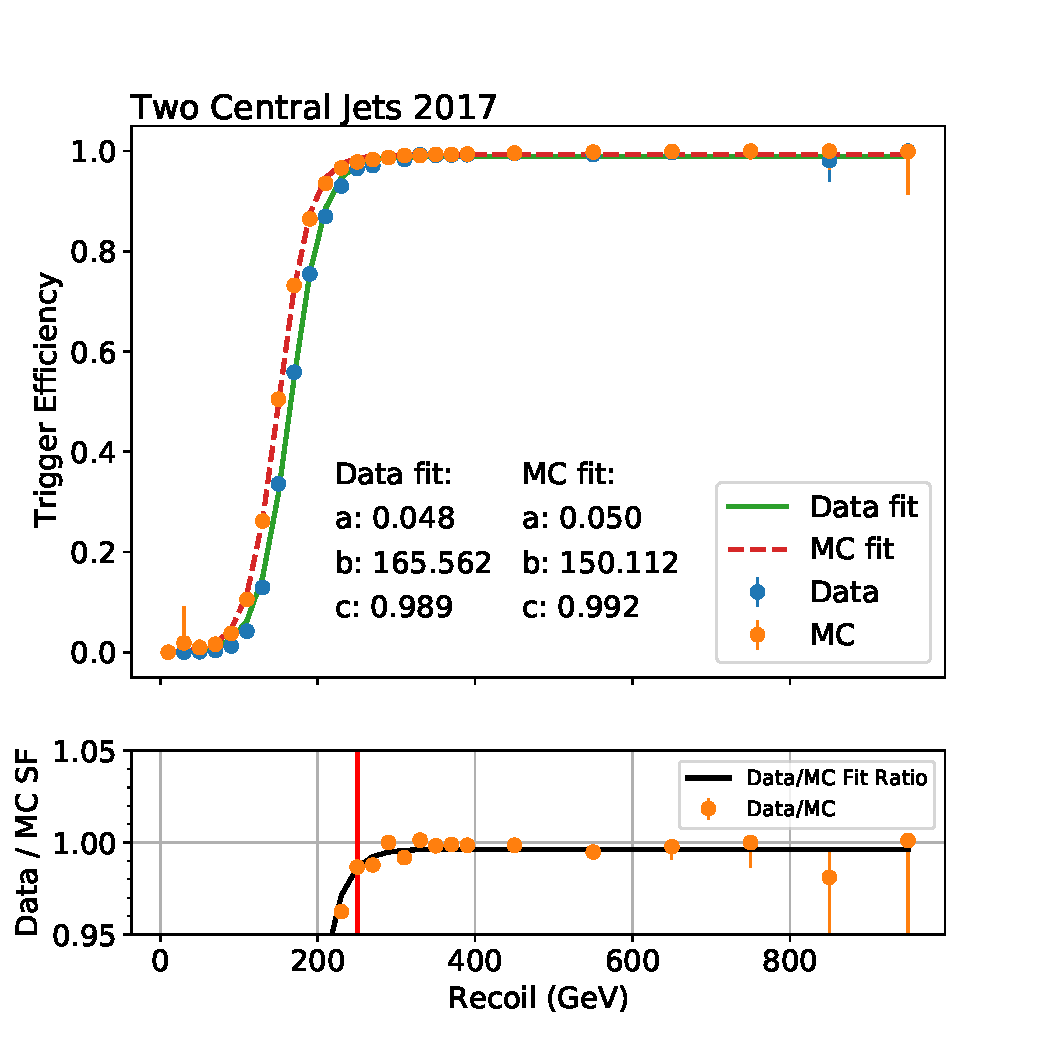
\includegraphics[width=0.49\textwidth]{Efficiency/METTrigger/eff_fit_two_central_jets_2017.pdf}
    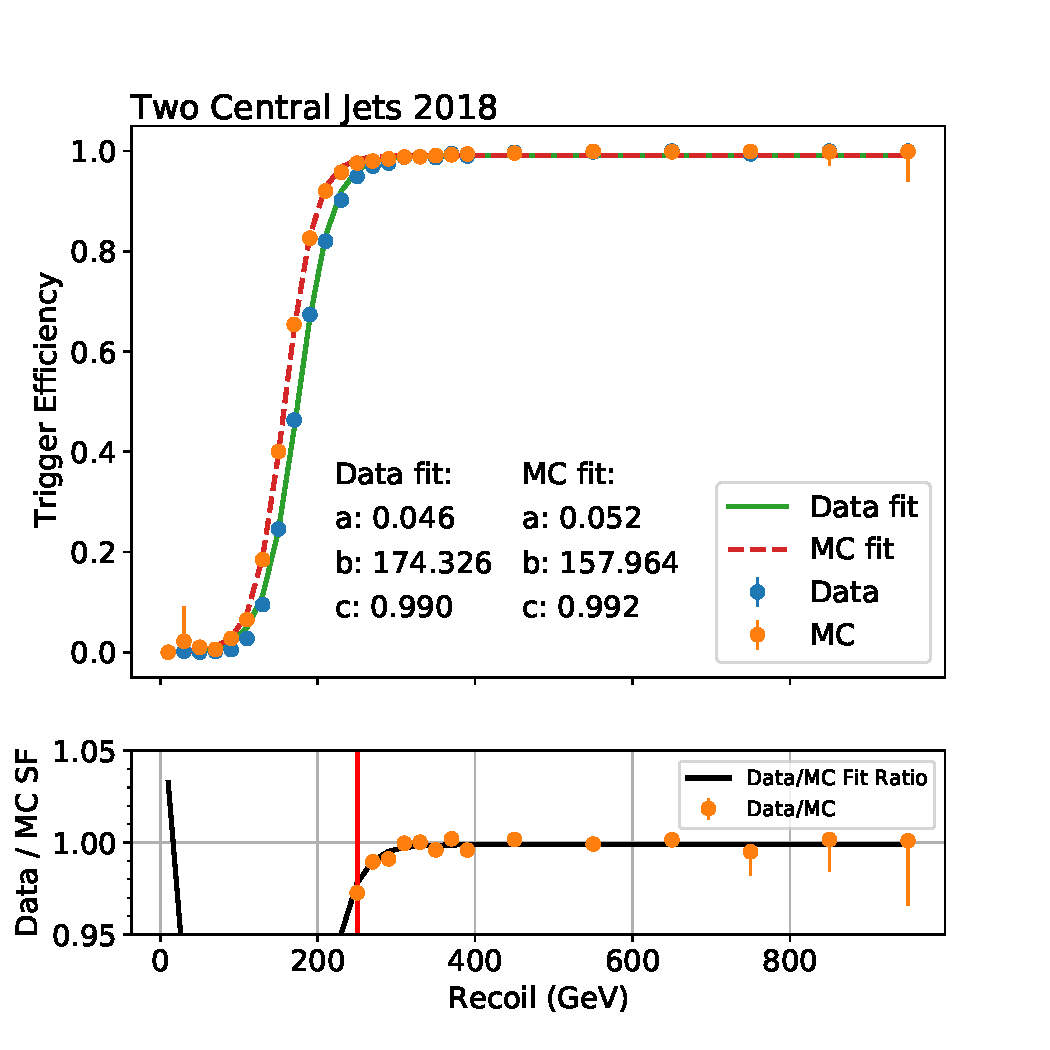
\includegraphics[width=0.49\textwidth]{Efficiency/METTrigger/eff_fit_two_central_jets_2018.pdf}
    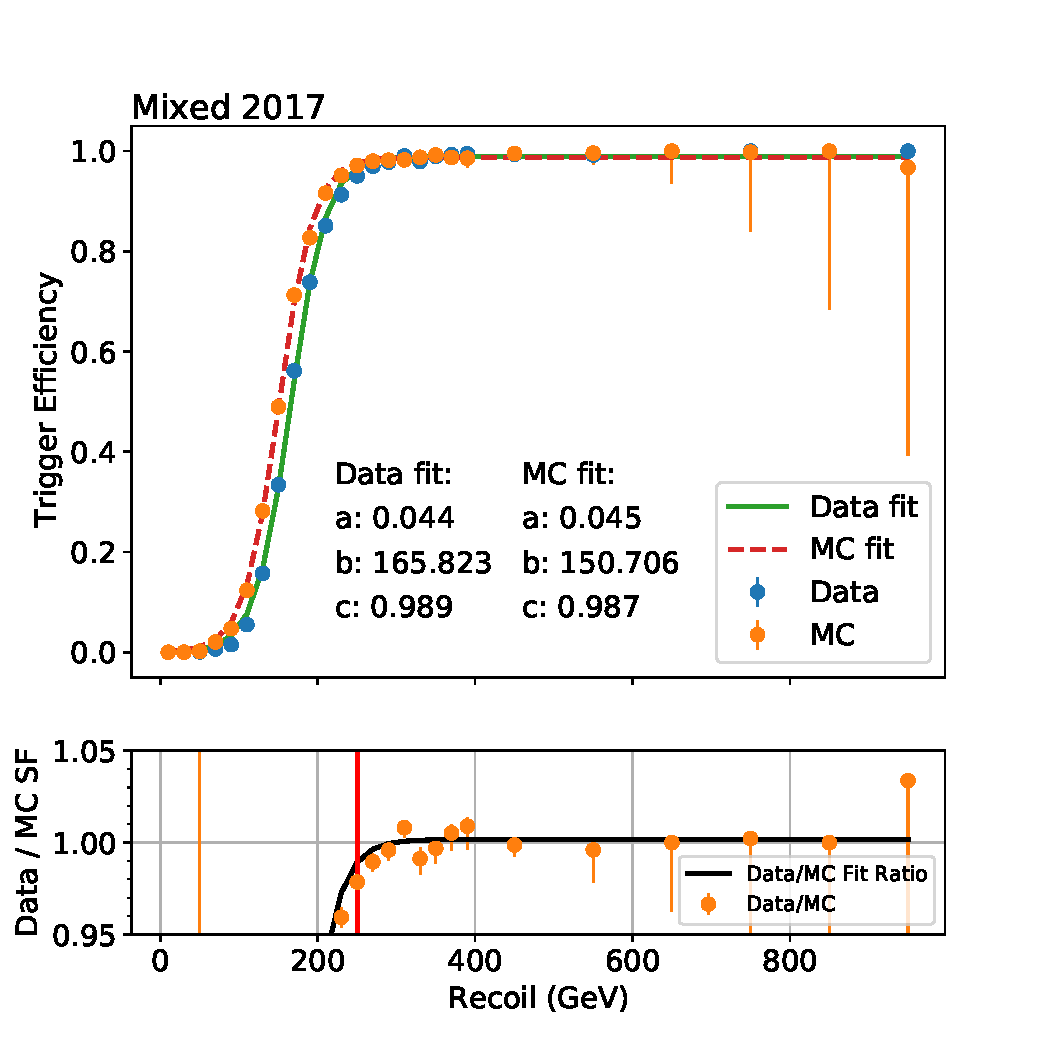
\includegraphics[width=0.49\textwidth]{Efficiency/METTrigger/eff_fit_one_jet_forward_one_jet_central_2017.pdf}
    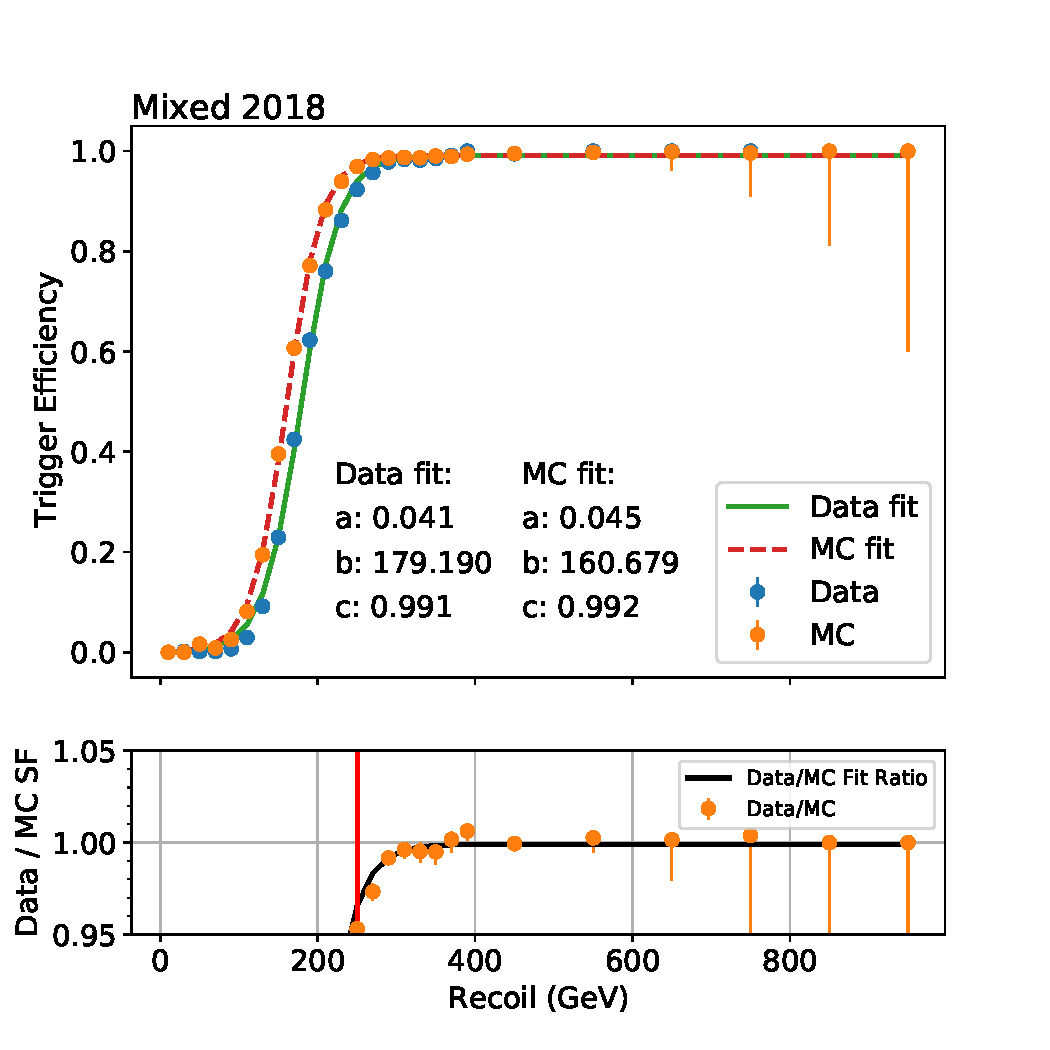
\includegraphics[width=0.49\textwidth]{Efficiency/METTrigger/eff_fit_one_jet_forward_one_jet_central_2018.pdf}
    \caption{MET trigger efficiencies for data and MC, for events where the two VBF jets are both central (top) 
    and where at least one jet is forward (bottom). Left column shows results with 2017 dataset, while the right column shows
    the results with 2018 dataset. To each efficiency curve, a sigmoid function 
    with three parameters are fitted: $f(x,a,b,c) = \frac{c}{1+e^{-a(x-b)}}$. 
    Resulting data/MC scale factors are shown in the bottom ratio pad for each case. The black line represents
    the ratio of two best-fit sigmoid functions, which is used as the correction factor to MC as a function of recoil.}
    \label{fig:sigmoid_fits_eff}
\end{figure}

\clearpage

\subsubsection{Photon trigger}
\label{subsubsec:photon_trig}

The photon trigger efficiency is measured using events collected with \texttt{HLT\_PFHT1050} 
trigger, which was fully unprescaled in 2017 and 2018, meaning that all the events passing the trigger were saved to the
disk.

Events are selected in the same way as for the photon control region in the analysis
(see Sec.~\ref{sec:selection_cr_g}) except for the photon $\pt$, recoil, $\HT$ and trigger requirements. To ensure an unbiased measurement, 
an offline $\HT$ of at least $1.5$ TeV is required, where $\HT$ is calculated as: 

\begin{equation}
  \HT = \sum_{jet} p_T^{jet}
  \label{eq:ht_def}
\end{equation}

In Eq.~\ref{eq:ht_def}, the sum runs over jets which pass the tight identification requirements 
and do not overlap with the selected photon within $\Delta R<0.4$. 
The trigger efficiency $\epsilon$ is then determined as:

$$\epsilon(\texttt{HLT\_Photon200}) = \frac{\text{Offline selection \&\& \texttt{HLT\_PFHT1050} \&\& 
\texttt{HLT\_Photon200}}}{\text{Offline selection \&\& \texttt{HLT\_PFHT1050}}} $$

The resulting efficiency in data and $\gamma +$jets \HT-binned simulation is shown in Fig.~\ref{fig:hlteff_photon}. In both data and simulation, 
the binned turn-on is fit using sigmoid functions, which are used to extract all further information. The trigger efficiencies in data and simulation are both 
found to be larger than $95\%$ for photon \pt values of more than $230$ GeV, which is used for the tight-identification requirement for photons reconstructed offline
(see Sec.~\ref{subsec:photons}). The MC-to-data scale factor is 
evaluated as the ratio of the sigmoid functions in data and simulation and is found to be within $1\%$ of unity consistent within an uncertainty of 1\% 
with all individual points. In the analysis implementation, the scale factor is implemented as an event-by-event weight based on the ratio of the sigmoid functions.

\begin{figure*}[hbtp]
    \begin{center}
        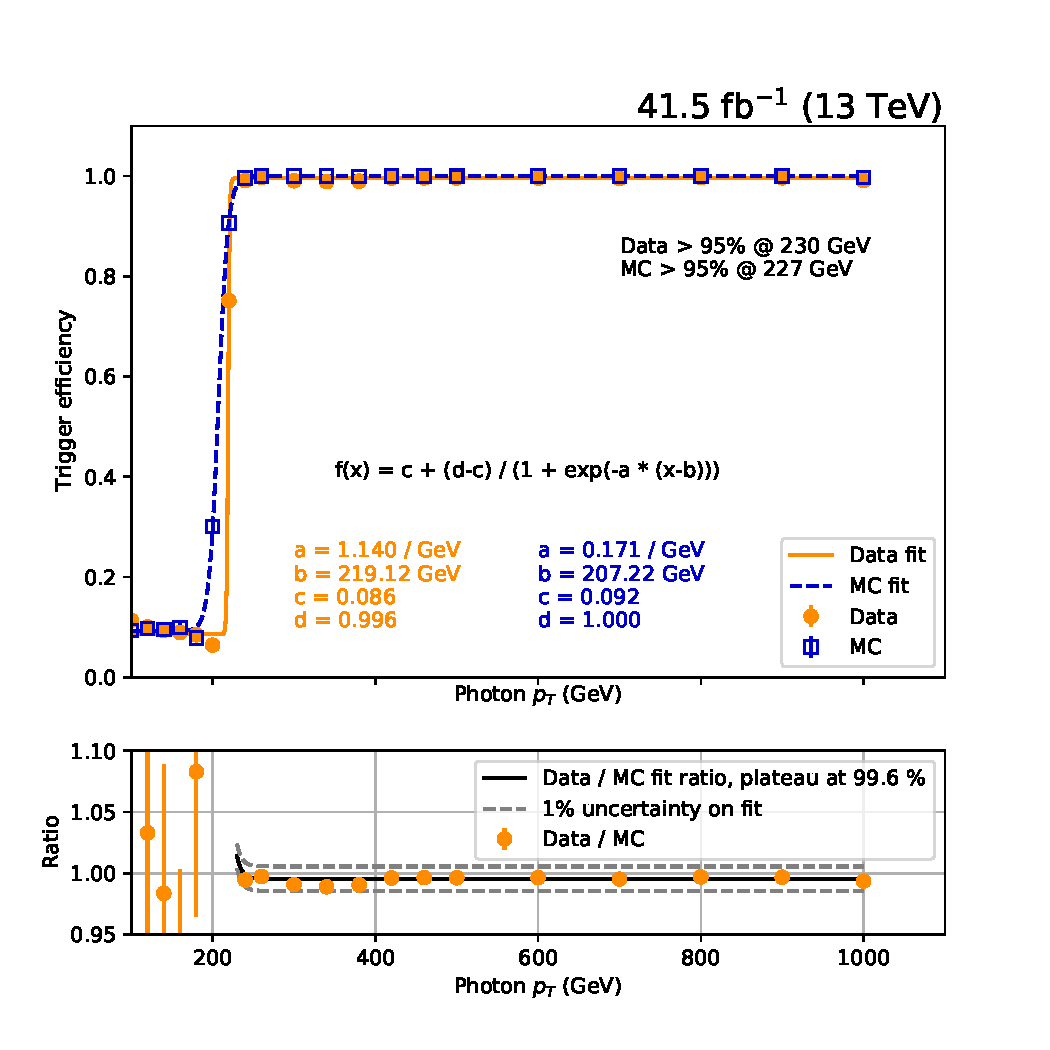
\includegraphics[width=0.6\textwidth]{Efficiency/Photon/fit_HLT_PFHT1050_2017.pdf}
        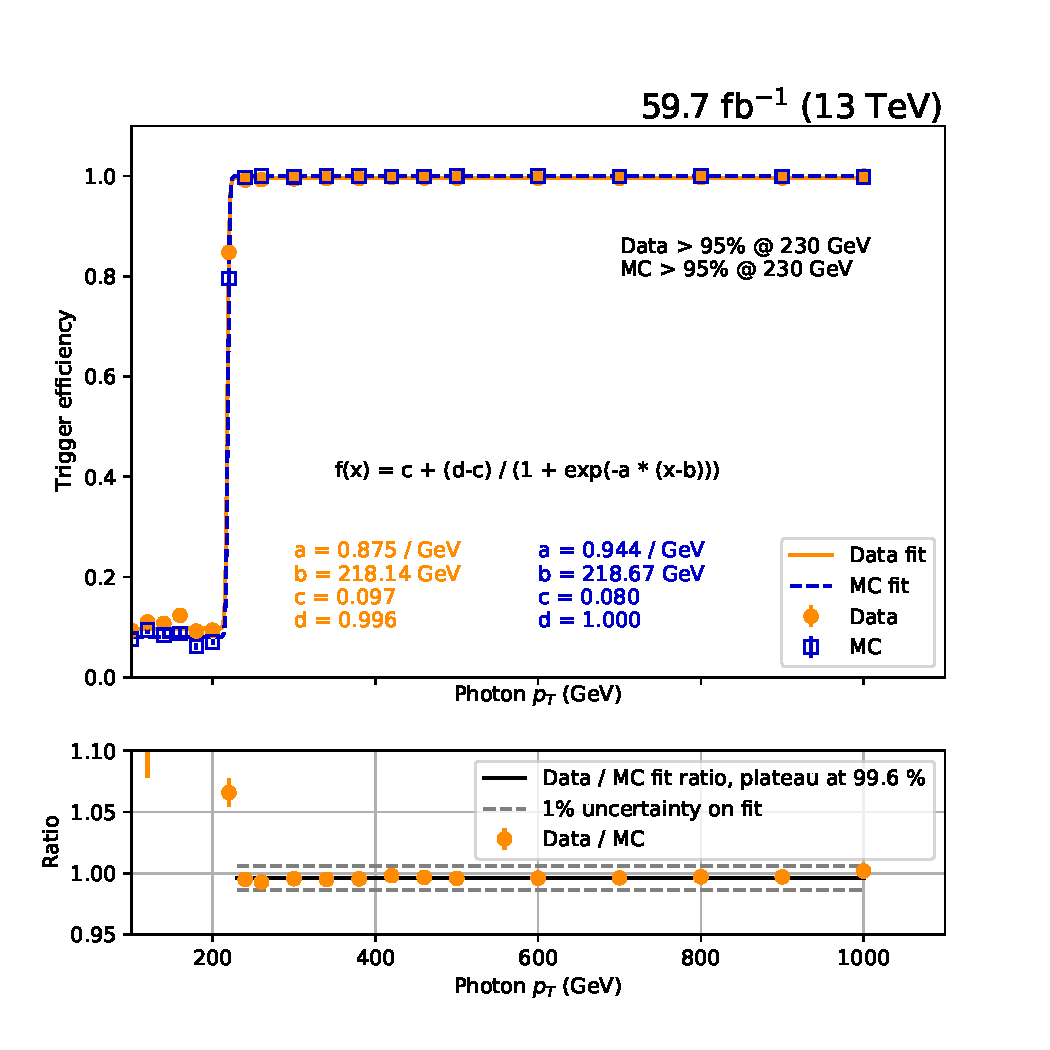
\includegraphics[width=0.6\textwidth]{Efficiency/Photon/fit_HLT_PFHT1050_2018.pdf}
        \caption{Efficiency of the \texttt{HLT\_Photon200} trigger in data and \HT-binned $\gamma+$jets MC for 2017 (top) and 2018 (bottom) 
        as a function of photon \pt. The orange and blue lines respectively represent sigmoid function fits to the turn-on in data and MC, 
        with the fit function and best-fit parameter values given in the respectively colored labels. The bottom panel shows the ratio of the values measured 
        in data over those in MC using orange markers. The solid black line corresponds to the ratio of the sigmoid fits to data and MC.}
        \label{fig:hlteff_photon}
    \end{center}
\end{figure*}

\clearpage

\subsubsection{Electron trigger}

This analysis uses the logical OR of three triggers for the selection of events with electrons in the final state:
\texttt{HLT\_Ele35*} (\texttt{HLT\_Ele32*}),
\texttt{HLT\_Ele115*} and \texttt{HLT\_Photon200} for 2017 (2018) data. The OR of these three triggers is henceforth referred to as ``the electron trigger'',
to simplify the discussion. The higher-threshold triggers are advantageous in that they either do not contain isolation requirements (\texttt{HLT\_Ele115}) or do not require 
a well-reconstructed track (\texttt{HLT\_Photon200}), both of which enhance the selection efficiency at large electron \pt.

The efficiency of the electron trigger is measured in data and simulation using a ``tag and probe'' method. Tag electrons are required to pass a 
logical OR of all triggers considered here. Both the tag electron and the probe electron are required to pass the tight identification criteria used for the analysis 
selection (see Tables~\ref{tab:tight_electron_def_barrel} and~\ref{tab:tight_electron_def_endcap}). In data, events are separated based on whether the probe electron passes 
the same trigger criteria as the tag. In both of these categories, 
separate fits to the distribution of the invariant mass of the tag-probe system are performed to extract the number of signal-like $Z(ee)$ events in each category, 
and the efficiency is defined as the ratio of the number of passing signal events and the number of all signal events. The efficiency in simulation is 
measured in a Drell-Yan sample, and the signal event counts are defined by simply counting all events in the passing and failing categories. The MC-to-data scale 
factor is then defined as the ratio of the efficiency in data and that in simulation. The efficiency in data, as well as the scale factors are shown in 
Fig.~\ref{fig:hlteff_electron}. Note the appearance of steps in the efficiency at electron momenta of $115$ and $200$ GeV, which are a result of the addition 
of the high-momentum triggers to the logical OR expression.

\begin{figure*}[hbtp]
    \begin{center}
    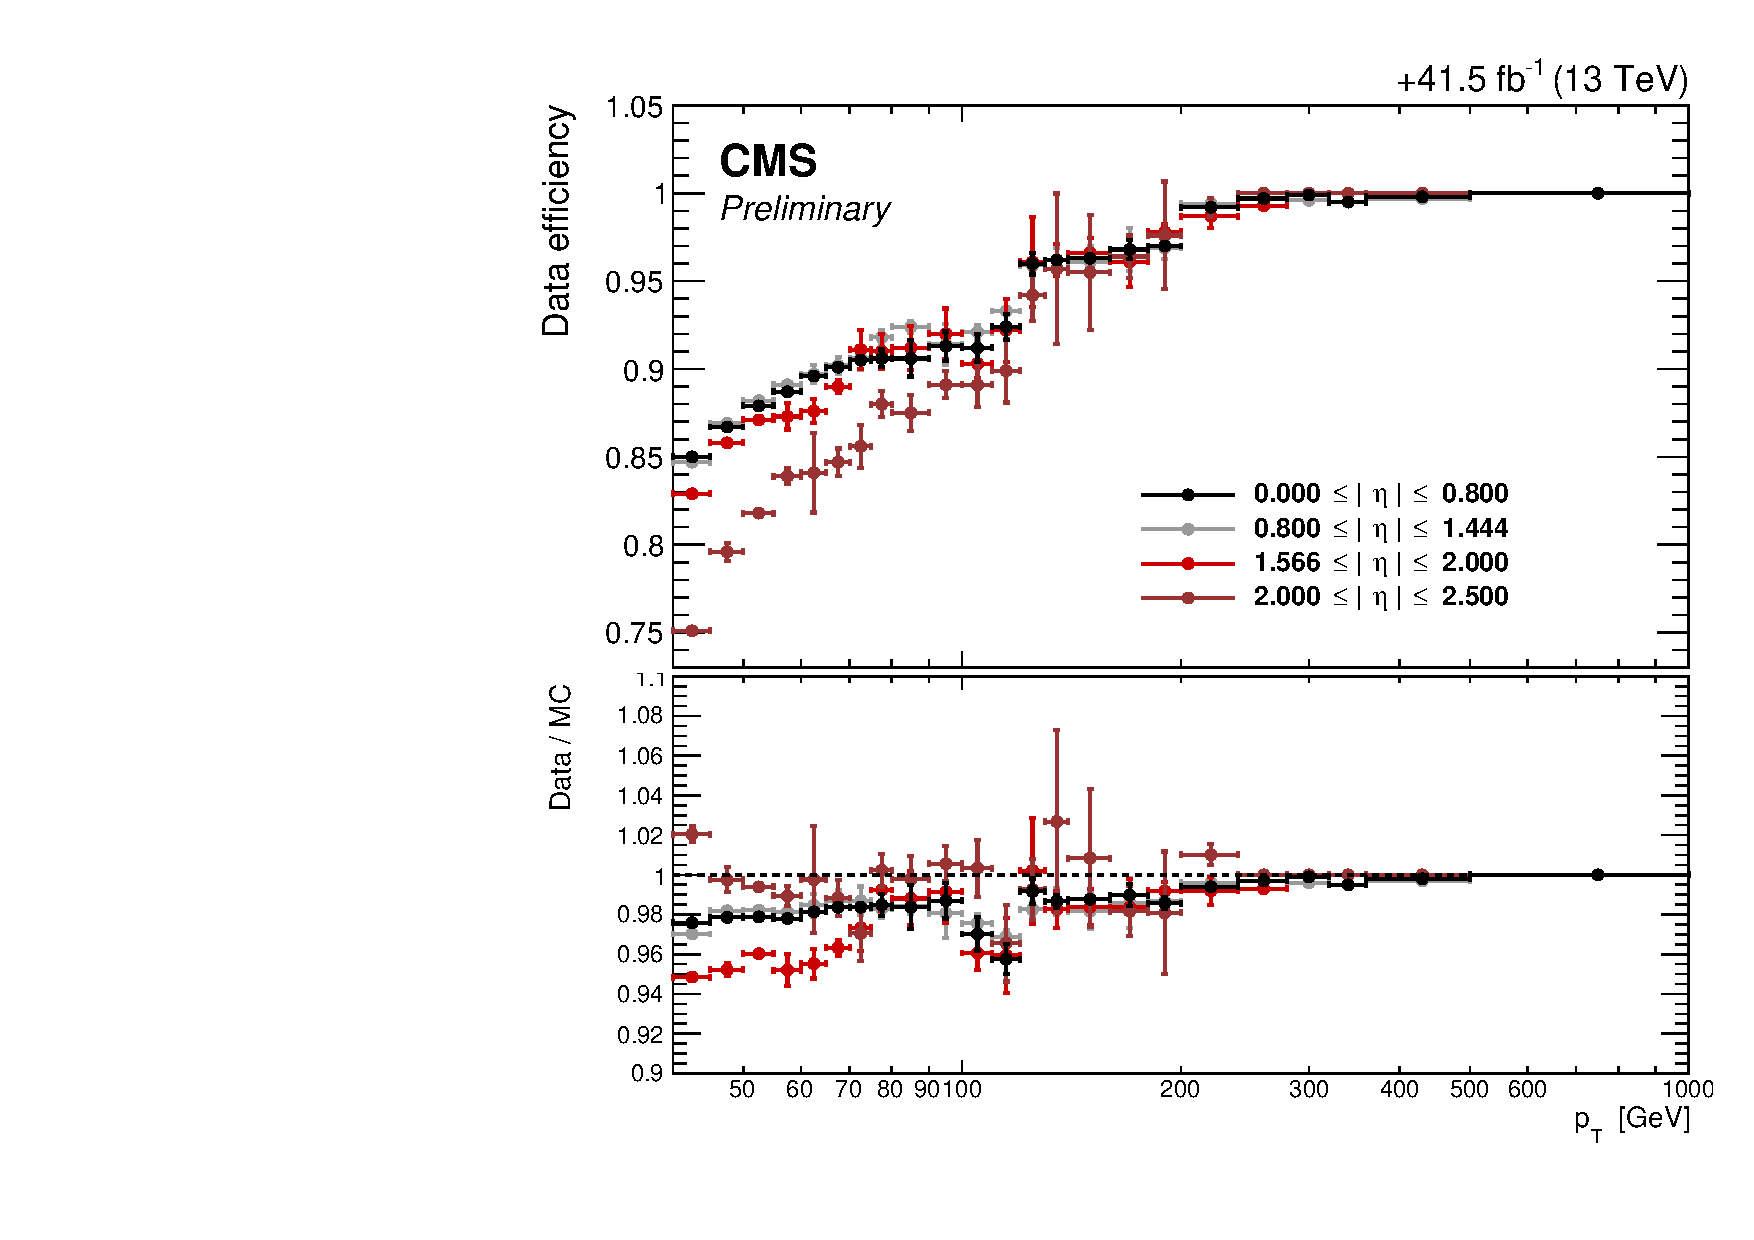
\includegraphics[width=0.6\textwidth]{Efficiency/Electron/electron_trig_eff_2017.pdf}
    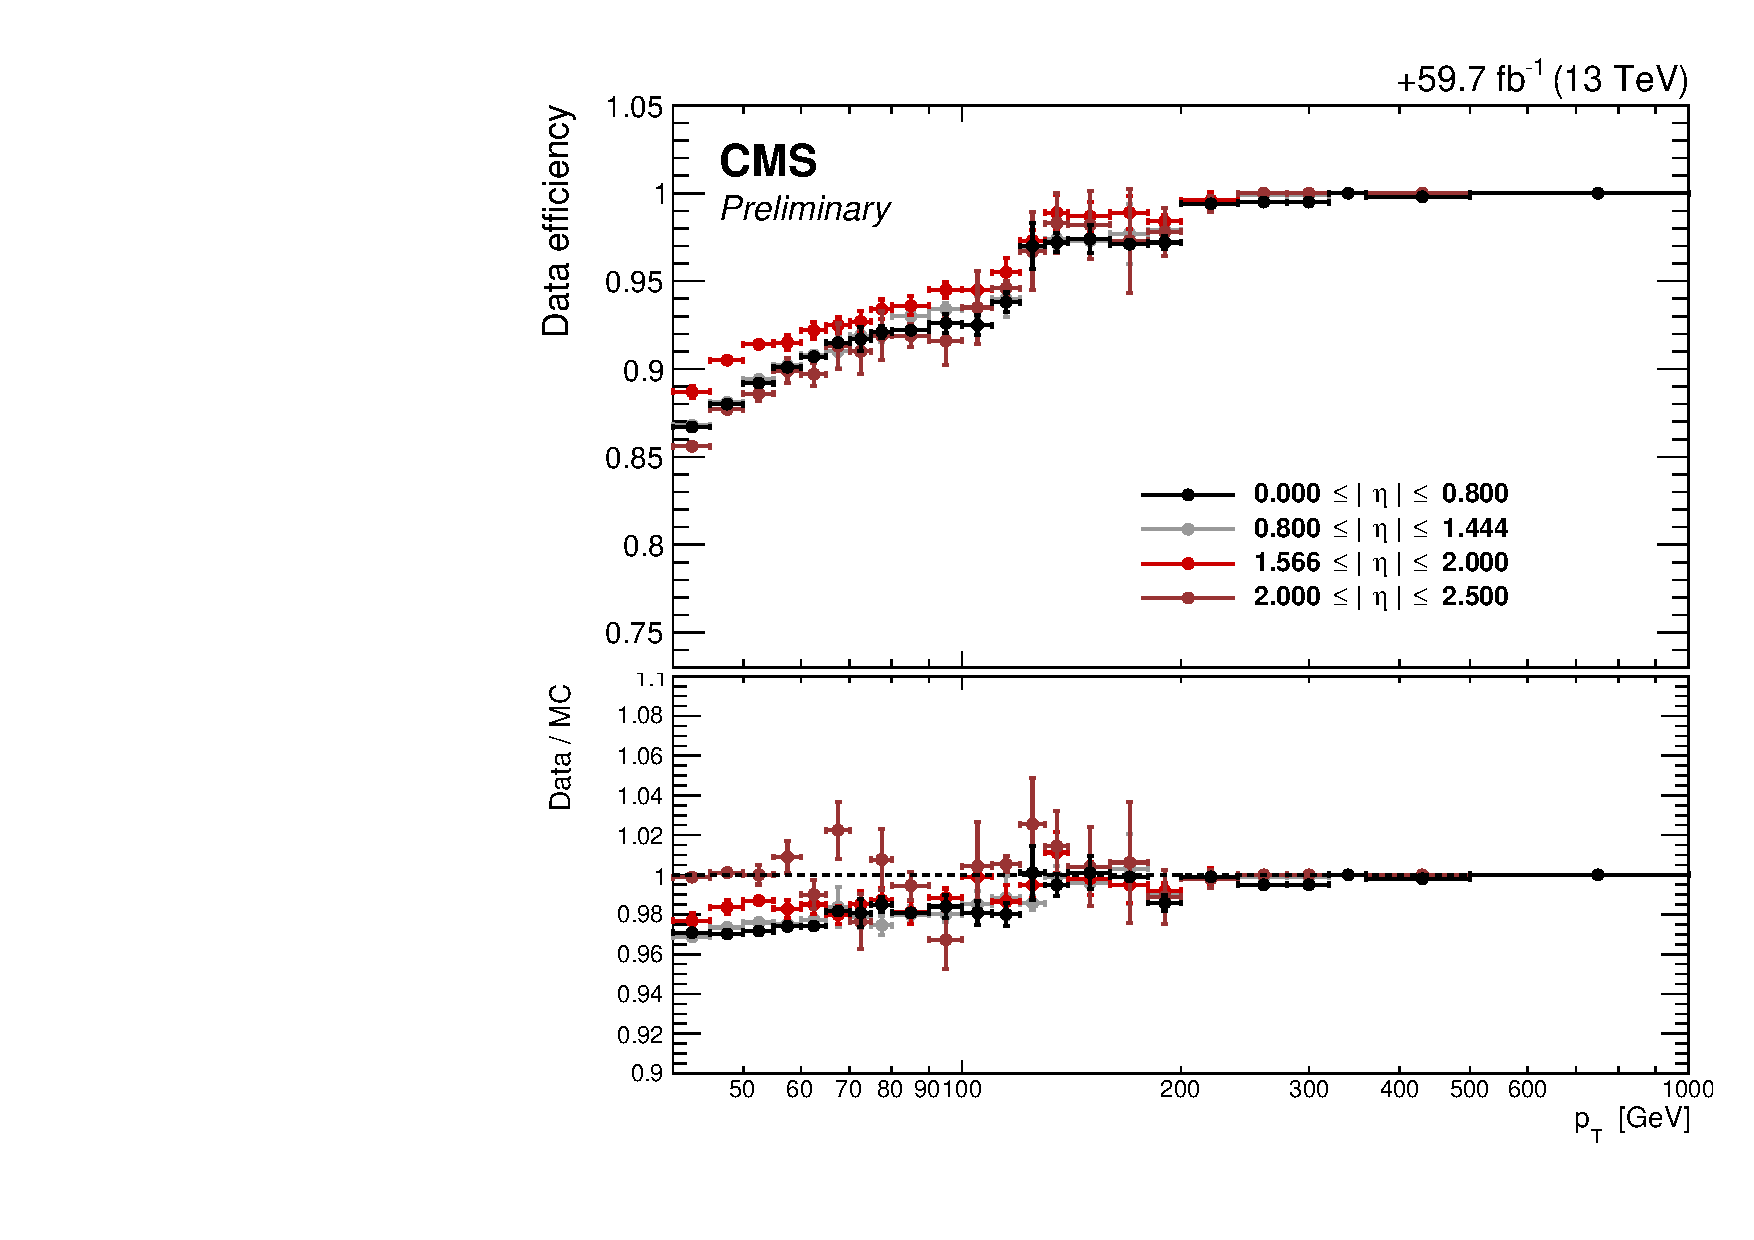
\includegraphics[width=0.6\textwidth]{Efficiency/Electron/electron_trig_eff_2018.pdf}
    \caption{Efficiency of the OR of the three triggers used to select electron events for 2017 (top) and 2018 (bottom) as a function of the electron 
        transverse momentum. The efficiency is shown for multiple regions of absolute electron pseudorapidity. In each plot, the upper panel shows 
        the efficiency in data, while the lower panel shows the ratio of the efficiency in data and that in simulation.}
    \label{fig:hlteff_electron}
    \end{center}
\end{figure*}

As shown in the bottom panel of Fig.~\ref{fig:hlteff_electron}, the data to MC scale factors are derived
from the two efficiency measurements from data and MC. Those correction factors are applied per-electron 
in the analysis to correct MC.

\subsection{Pileup reweighting}
\label{subsec:pu_reweighting}

The pileup (PU) conditions\footnote{The term ``pileup conditions'' refers to the distribution 
of the number of reconstructed p-p collision vertices in a given p-p bunch crossing.} 
in the simulated samples are not identical to the ones observed in data, and a per-event reweighting is applied to remove the difference.
The reweighting is performed by matching the true pileup distribution of each simulated sample
with the pileup distribution in data. The pileup distribution in data is obtained through 
the pileupCalc tool, assuming a minimum bias cross section of 69.2$\pm 4.6\%$~mb, following the recommendations in \cite{pileup_twiki}.
The true pileup distributions in data and simulation are shown in Fig.~\ref{fig:purwg_true}, which show the normalized number of events as a function of 
the number of reconstructed collision vertices. 
The distribution of the number of reconstructed vertices 
for $W\to \mu\nu$ events before and after PU reweighting is shown in Fig.~\ref{fig:purwt_npv}. The distribution of the event energy density 
$\rho$ is shown in Fig.~\ref{fig:purwt_rho}, again before and after PU reweighting. 
In terms of these two variables, it is observed that PU reweighting improves the agreement between data and MC.

\begin{figure}[ht!]
  \begin{center}
    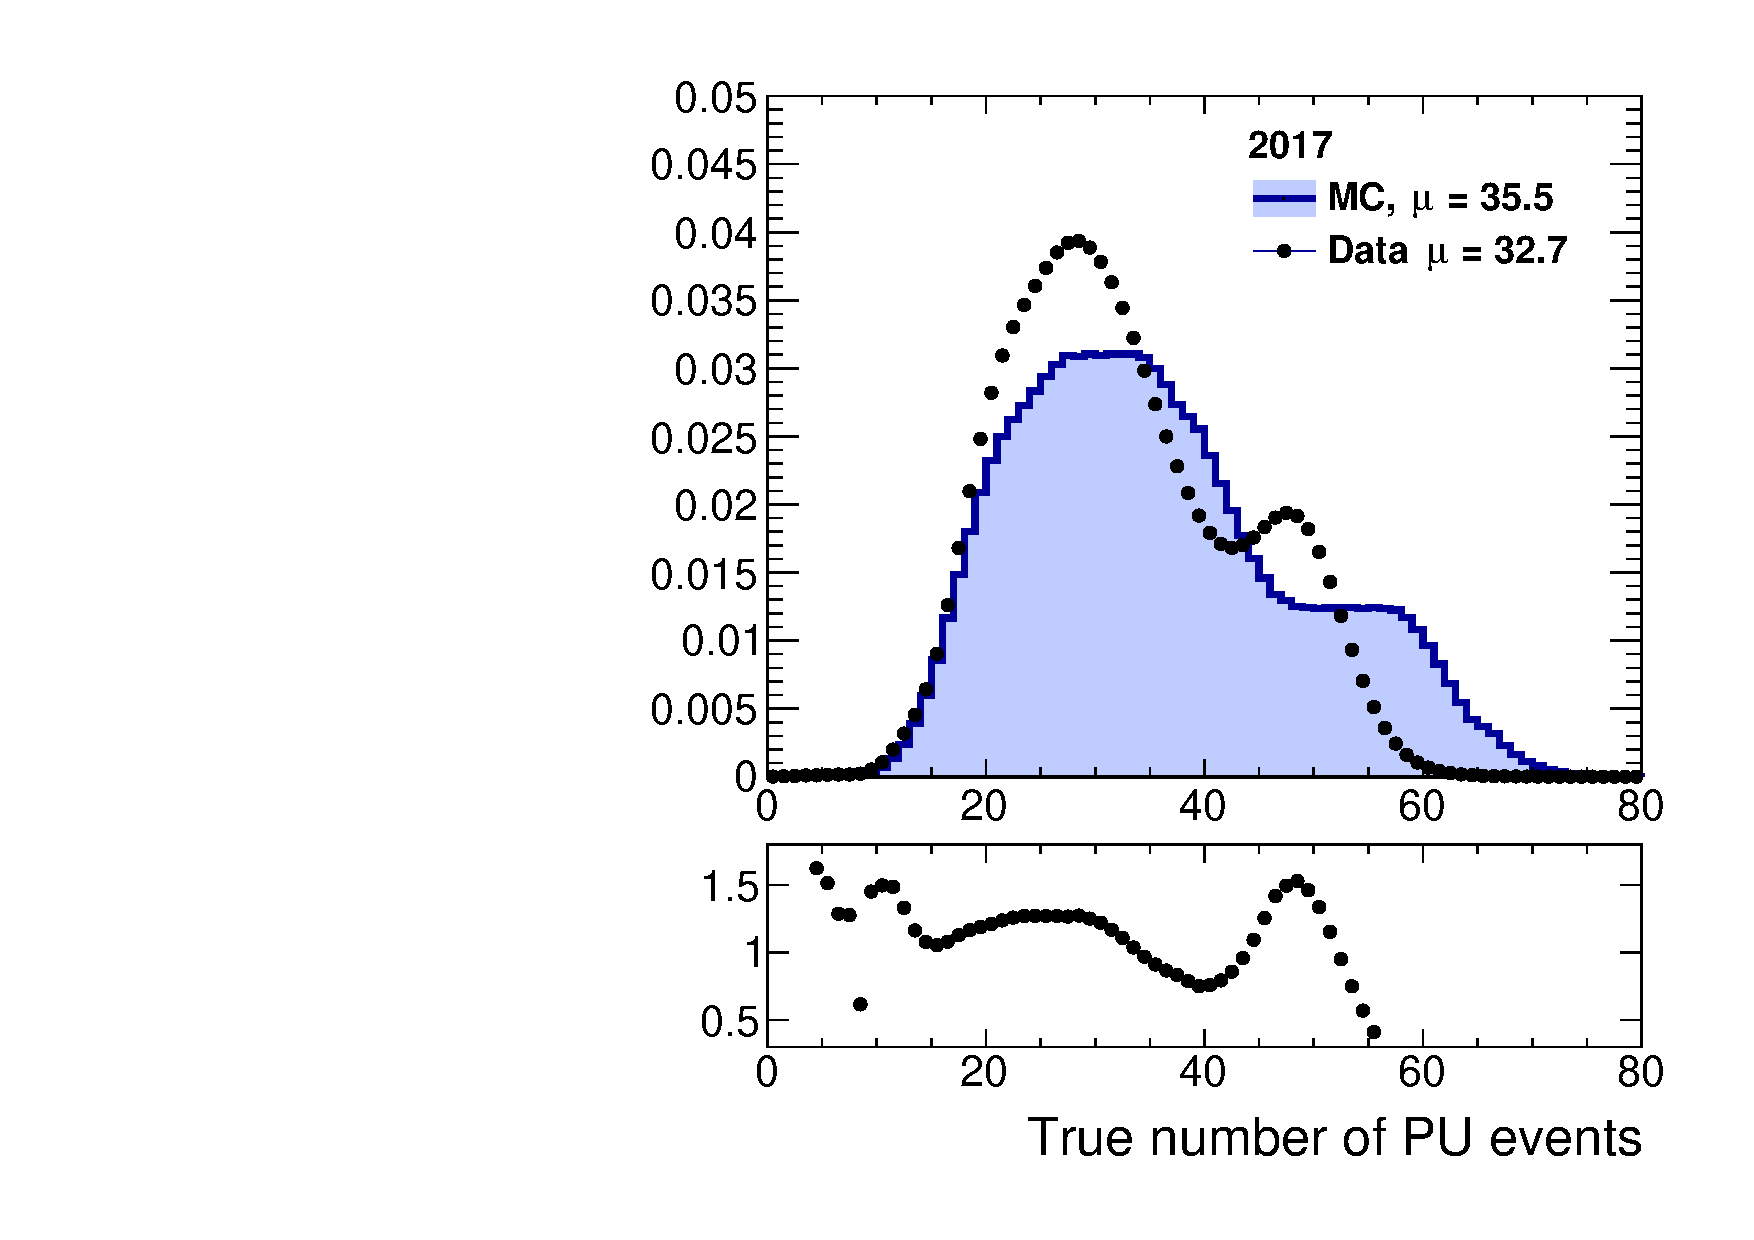
\includegraphics[width=0.49\textwidth]{Pileup/pu_weights_2017.pdf}
    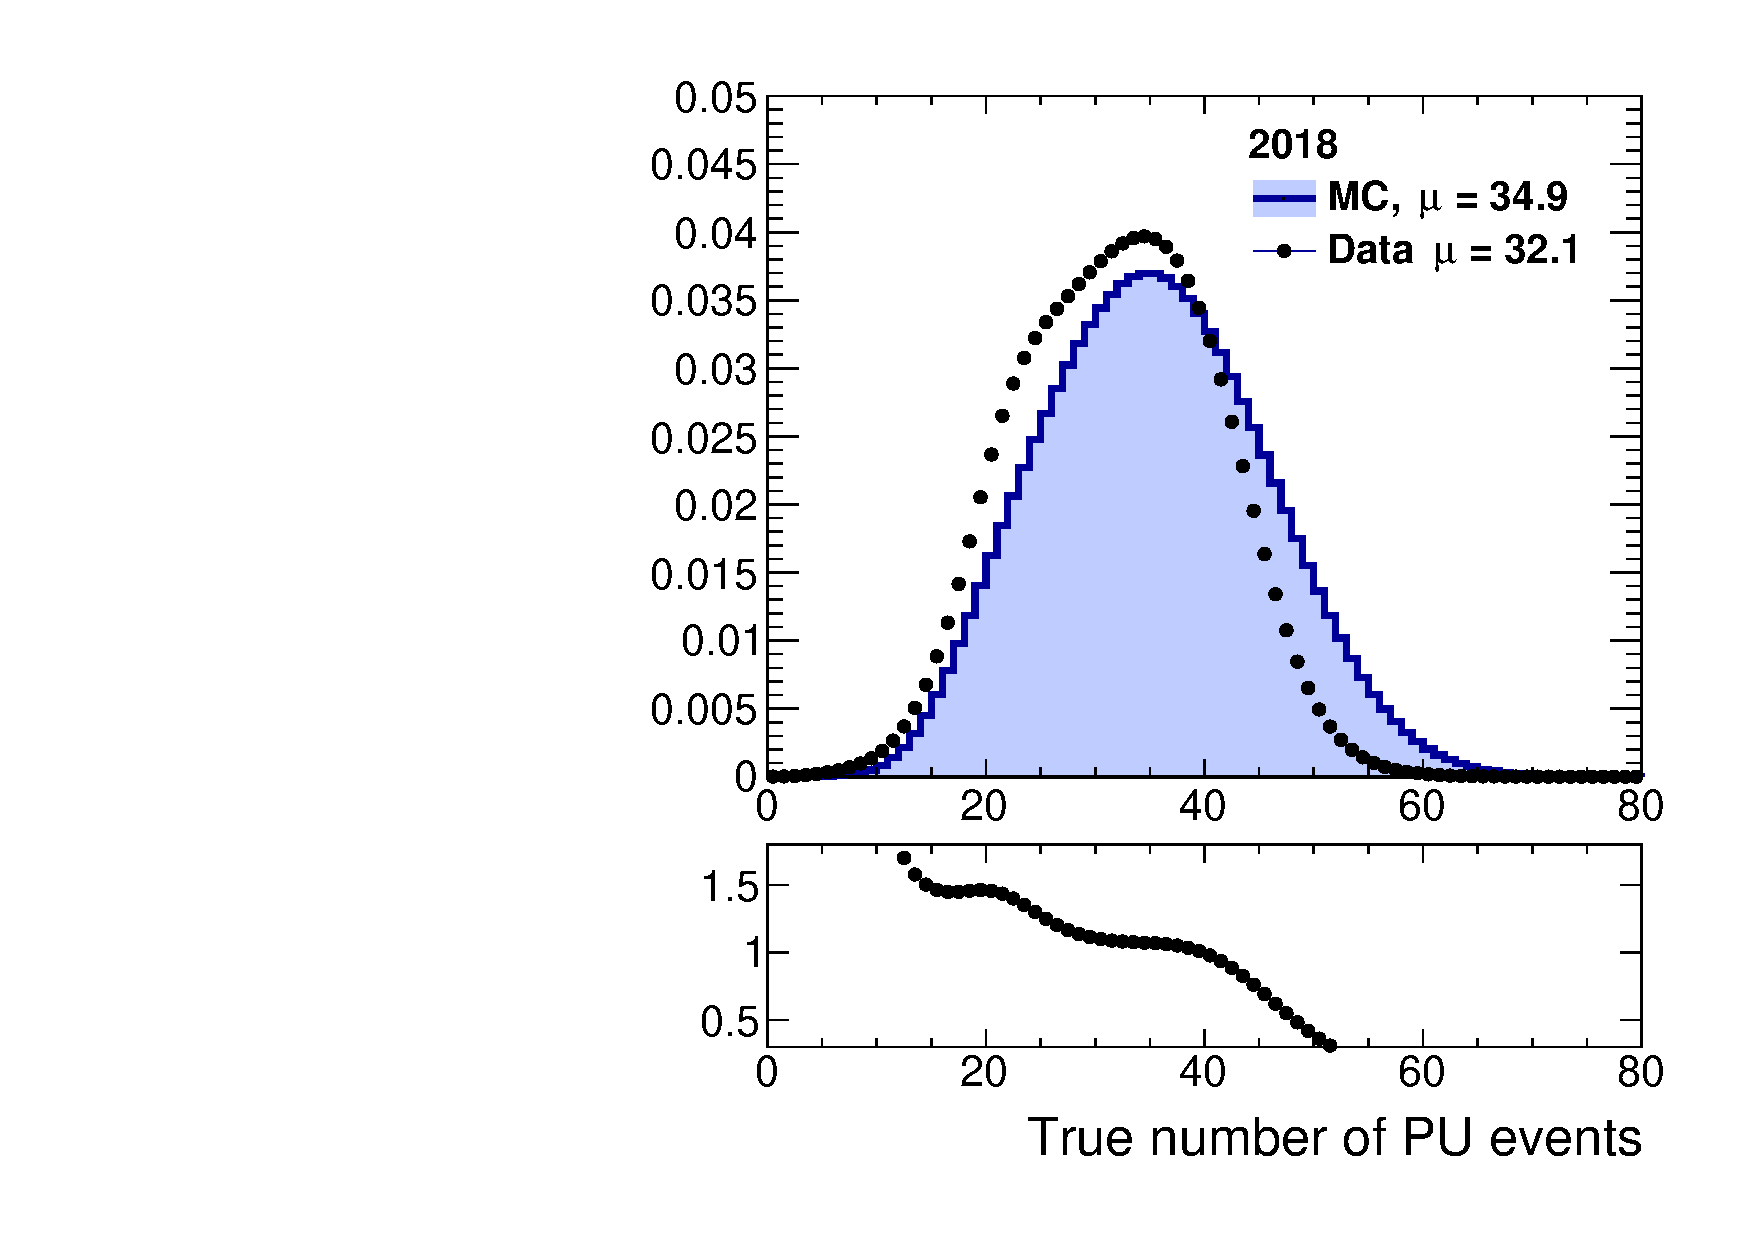
\includegraphics[width=0.49\textwidth]{Pileup/pu_weights_2018.pdf}
    \caption{
        Distribution of the true number of PU events in data and simulation for 2017 (left) and 2018 (right).
        The distributions for data are extracted assuming a minimum bias cross section of $69.2~\mathrm{mb}$.
    }
    \label{fig:purwg_true}
  \end{center}
\end{figure}

\begin{figure}[ht!]
  \begin{center}
    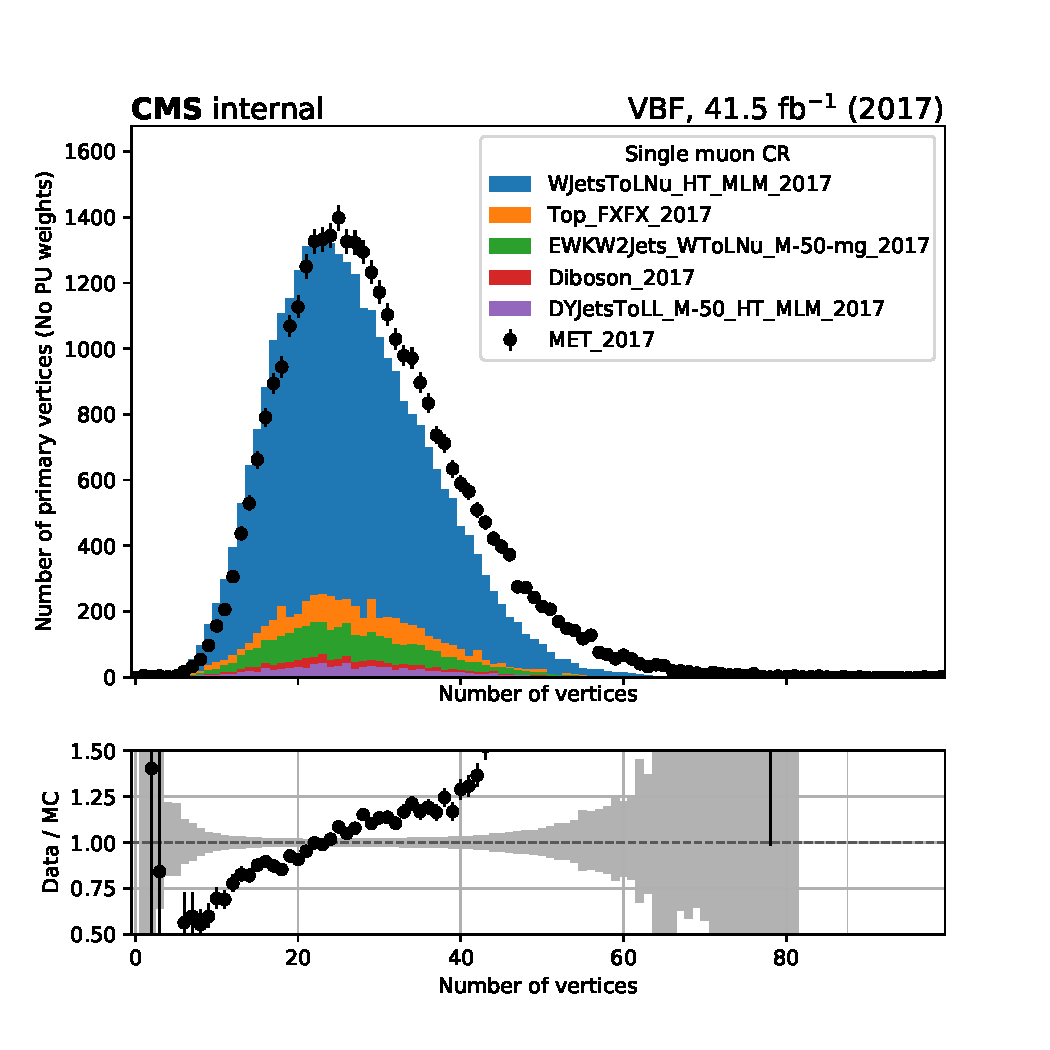
\includegraphics[width=0.49\textwidth]{Pileup/cr_1m_vbf_npv_nopu_2017.pdf}
    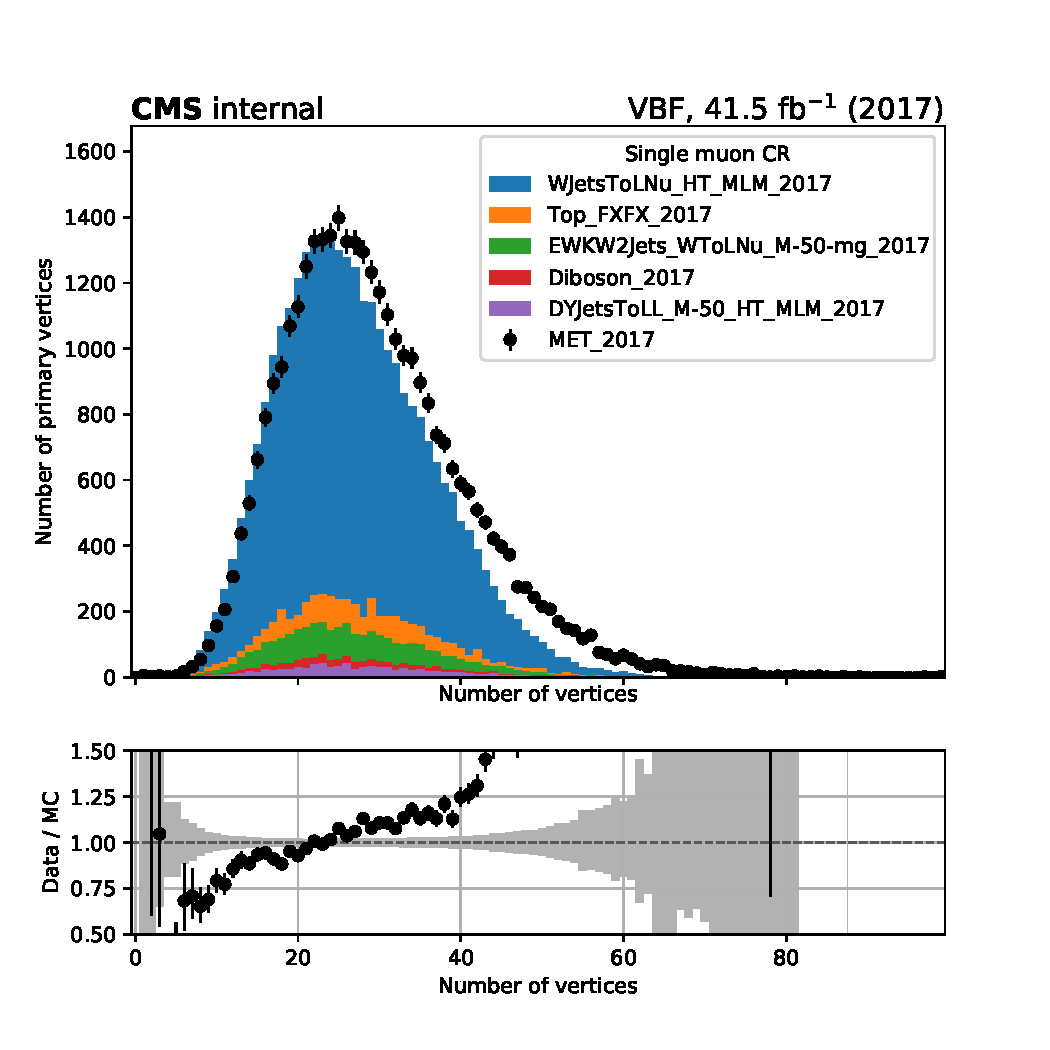
\includegraphics[width=0.49\textwidth]{Pileup/cr_1m_vbf_npv_2017.pdf}
    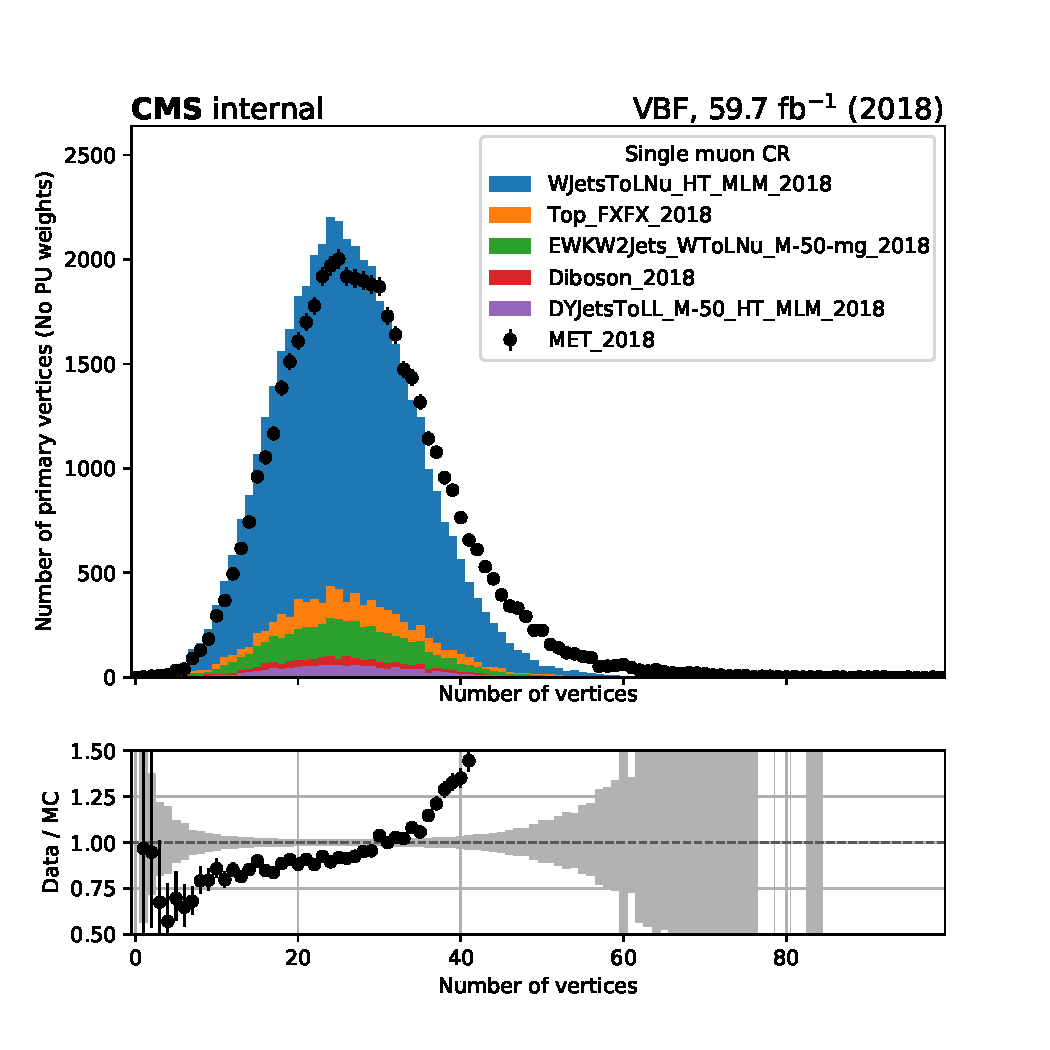
\includegraphics[width=0.49\textwidth]{Pileup/cr_1m_vbf_npv_nopu_2018.pdf}
    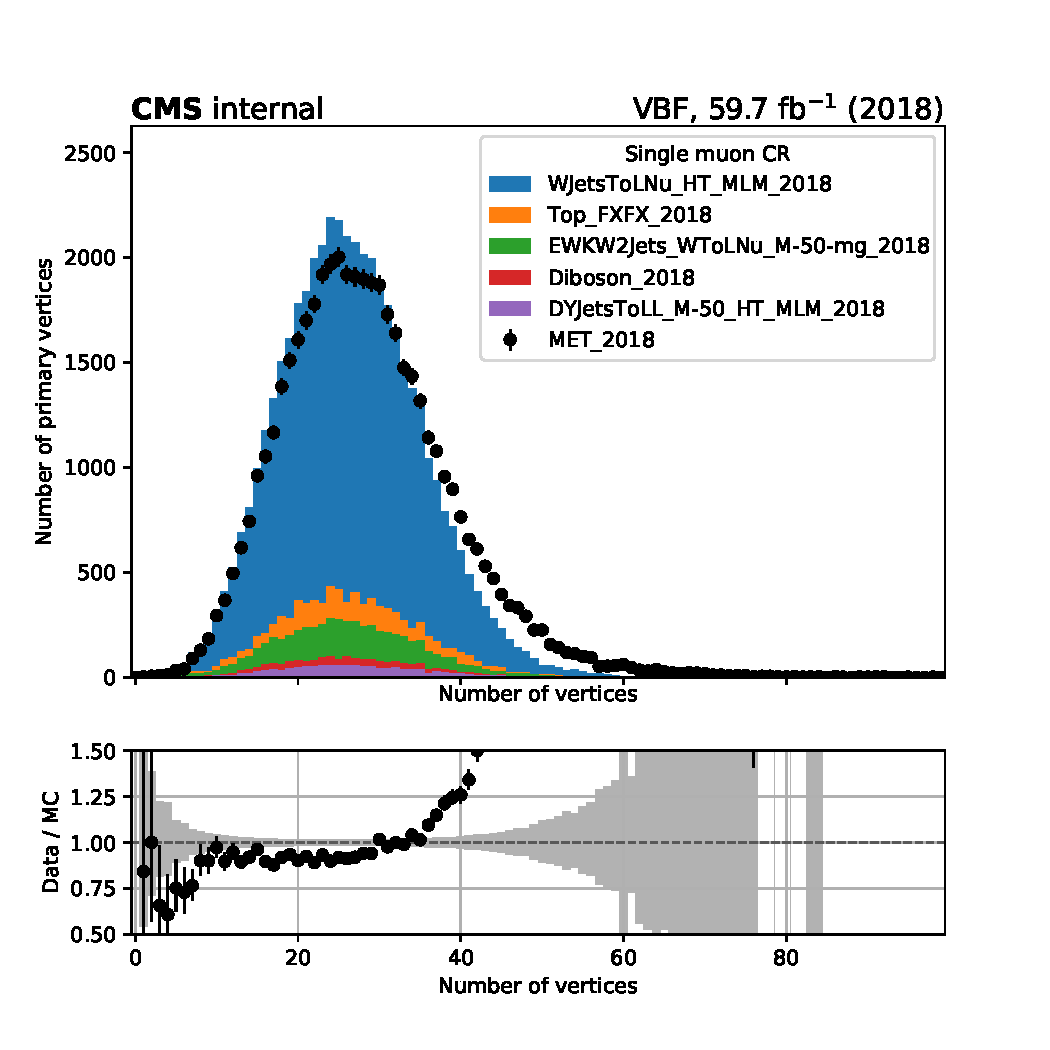
\includegraphics[width=0.49\textwidth]{Pileup/cr_1m_vbf_npv_2018.pdf}
    \caption{
        Distribution of the number of vertices in \Wmn~events in data and
        simulation before pileup re-weighting (left) and after pileup reweighting (right).
        The Monte Carlo is normalized to the luminosity of 41.5 and 59.7 fb$^{-1}$, respectively for 2017 and 2018.
    }
    \label{fig:purwt_npv}
  \end{center}
\end{figure}

\begin{figure}[ht!]
  \begin{center}
    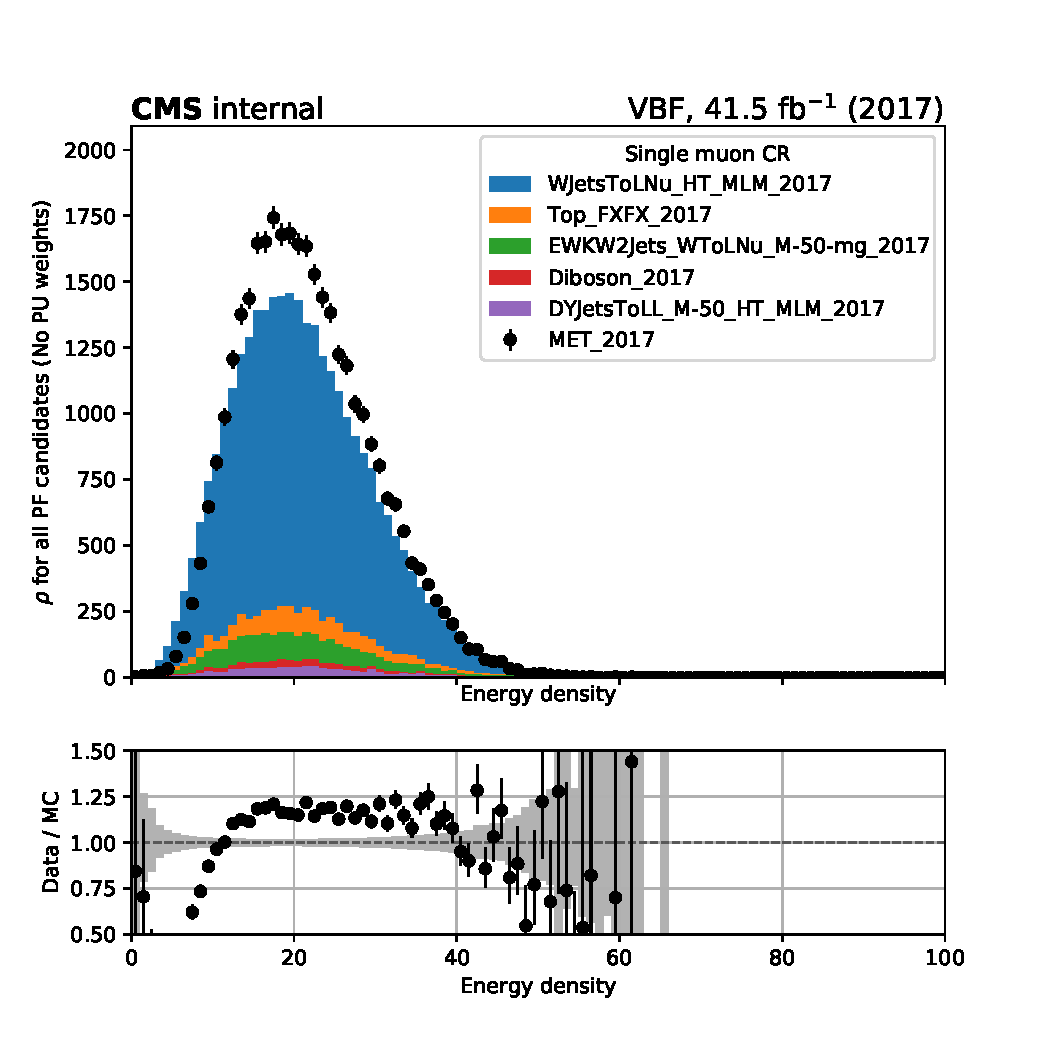
\includegraphics[width=0.49\textwidth]{Pileup/cr_1m_vbf_rho_all_nopu_2017.pdf}
    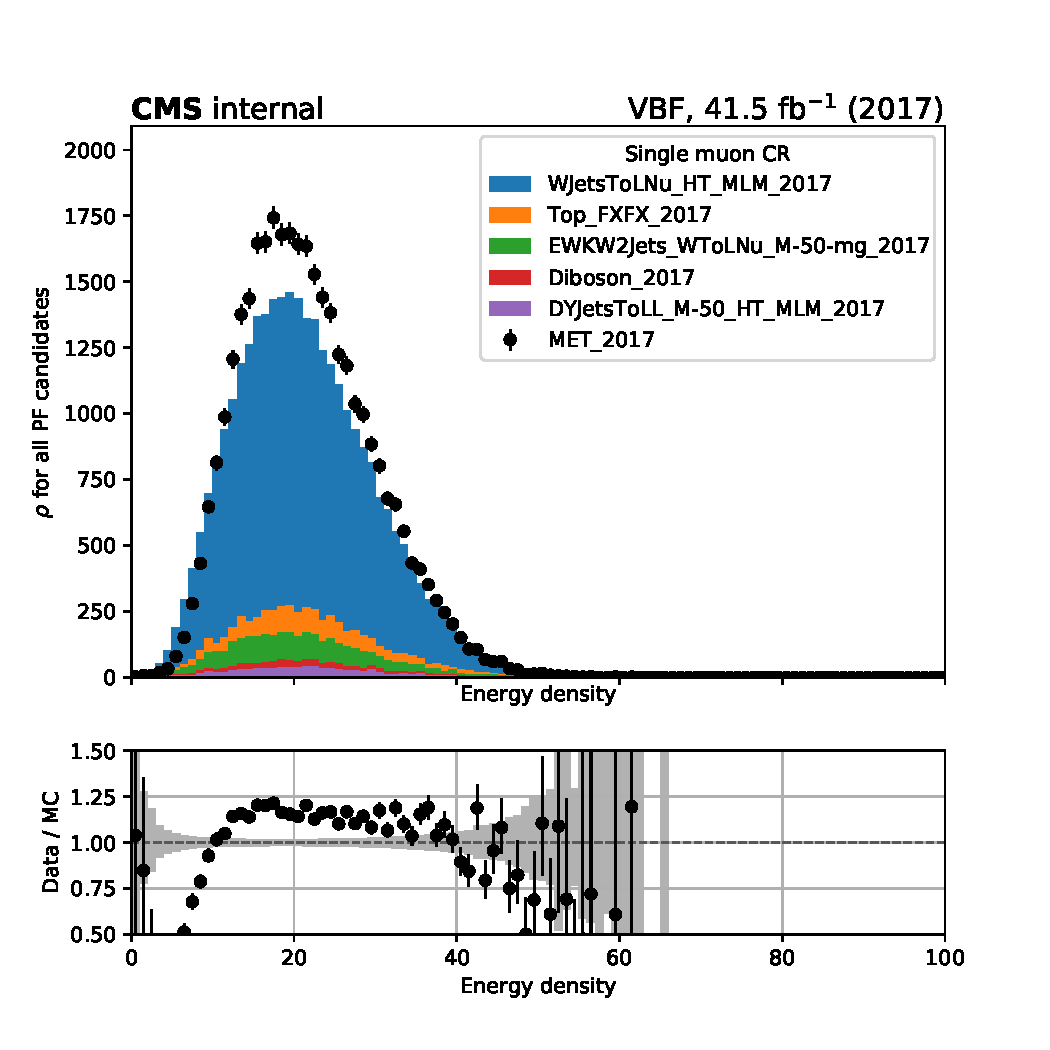
\includegraphics[width=0.49\textwidth]{Pileup/cr_1m_vbf_rho_all_2017.pdf}
    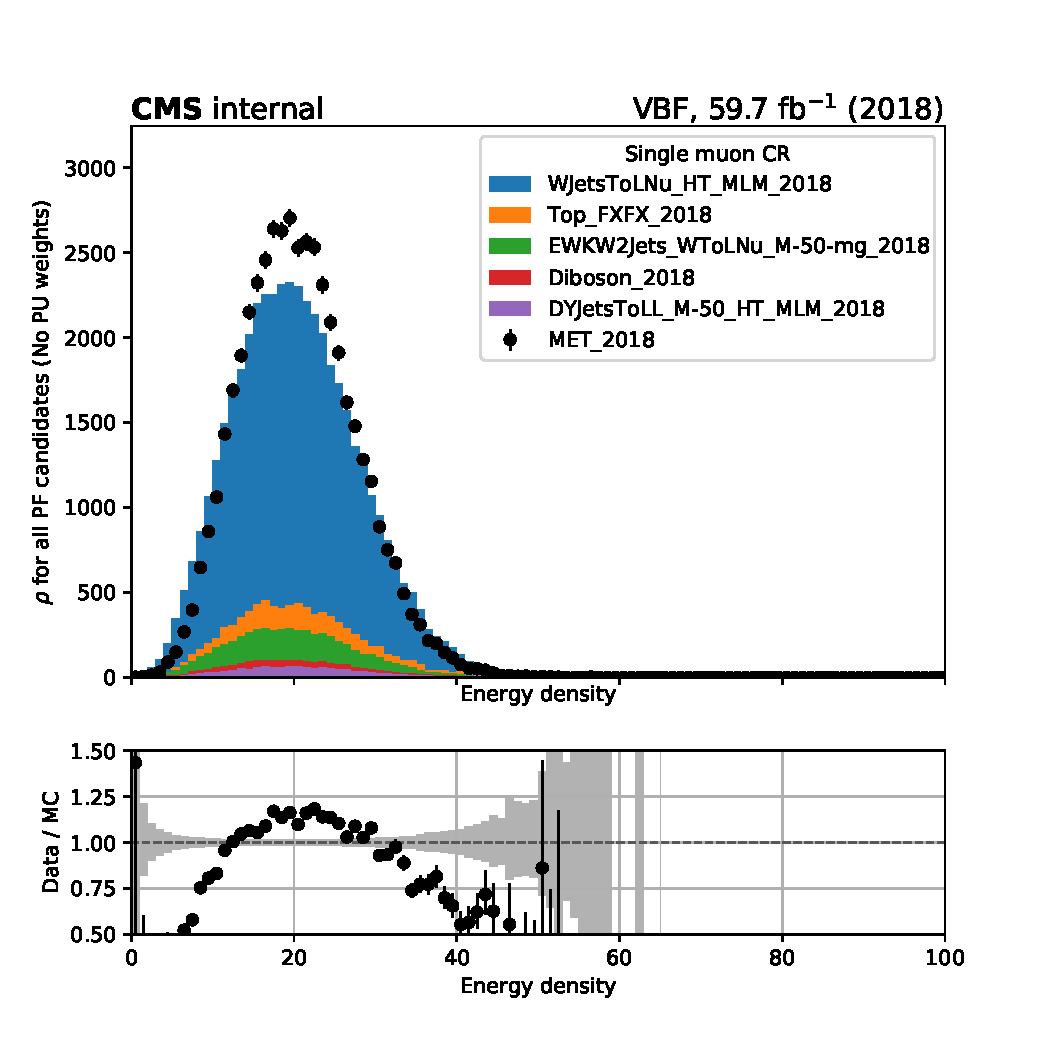
\includegraphics[width=0.49\textwidth]{Pileup/cr_1m_vbf_rho_all_nopu_2018.pdf}
    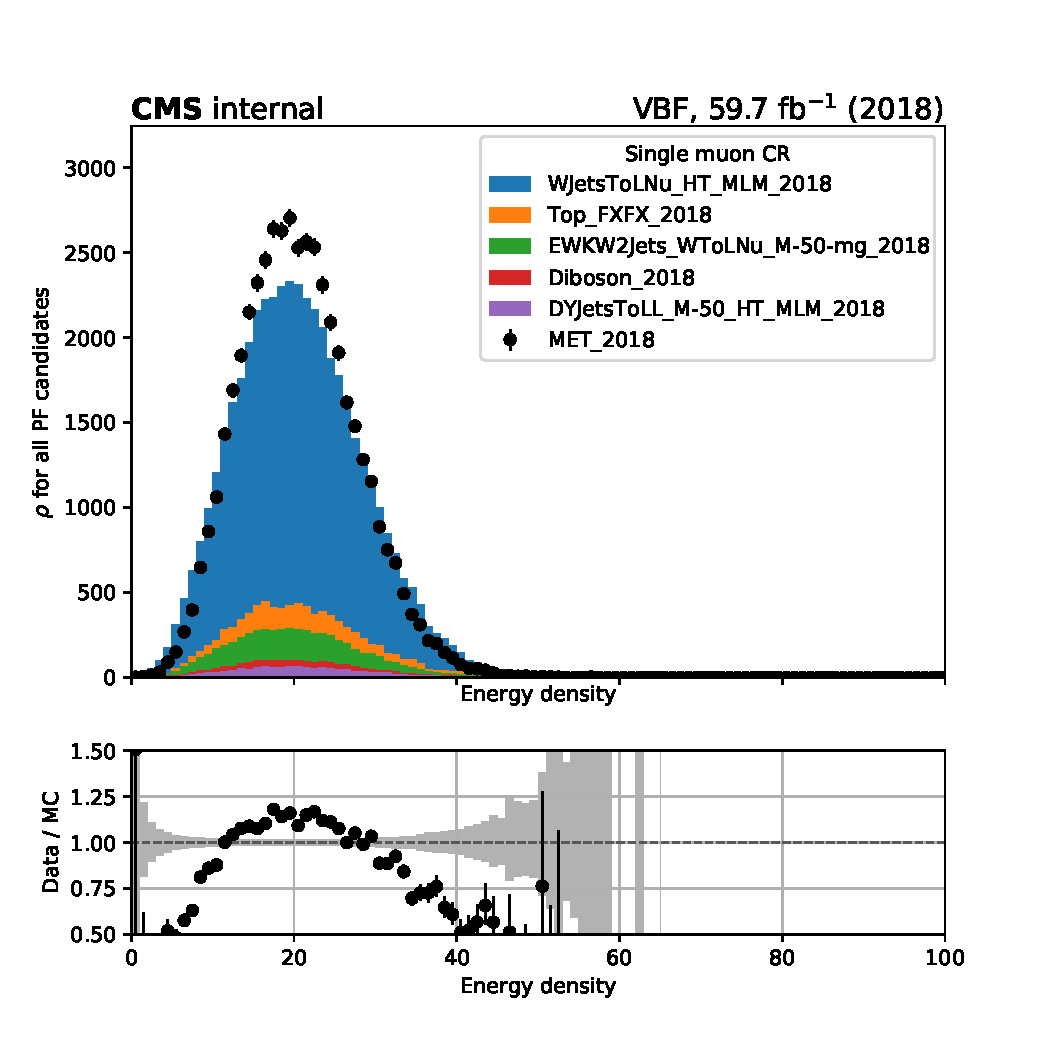
\includegraphics[width=0.49\textwidth]{Pileup/cr_1m_vbf_rho_all_2018.pdf}
    \caption{
        Distribution of the event energy density $\rho$ in \Wmn~events in data and
        simulation before pileup re-weighting (left) and after pileup reweighting (right).
        The Monte Carlo is normalized to the luminosity of 41.5 and 59.7 fb$^{-1}$, respectively for 2017 and 2018.
    }
    \label{fig:purwt_rho}
  \end{center}
\end{figure}

\clearpage

\subsection{Lepton identification efficiency reweighting}
\label{subsec:lepton_id_reweighting}

Data-to-MC scale factors are applied to events in the control regions to
account for differences in the reconstruction, identification and isolation of leptons
between data and MC. These data-to-MC scale factors are derived from the efficiencies that are measured for the electron and muon
selections in bins of $\pt$ and $\eta$ in both data and MC. The muon reconstruction and identification scale factors are
provided by the relevant POGs. Electron identification scale factors are measured using a tag-and-probe method, and the results are reviewed 
and approved by EGamma POG.

The reconstruction scale factors for electrons are shown in Fig.~\ref{fig:sf_electron_reco}. The corresponding identification scale factors for 
veto and tight electrons are shown in Fig.~\ref{fig:sf_electron_id}, and include the effect of the isolation efficiency. 

The identification scale factors for muons are shown in Fig.~\ref{fig:sf_muon_id}. Here, isolation scale factors are applied separately and are 
shown in Fig.~\ref{fig:sf_muon_iso}. The corresponding corrections for muons are deemed negligible~\cite{CMS-MUO-TWIKI-SF}.

\begin{figure}[ht!]
  \begin{center}
    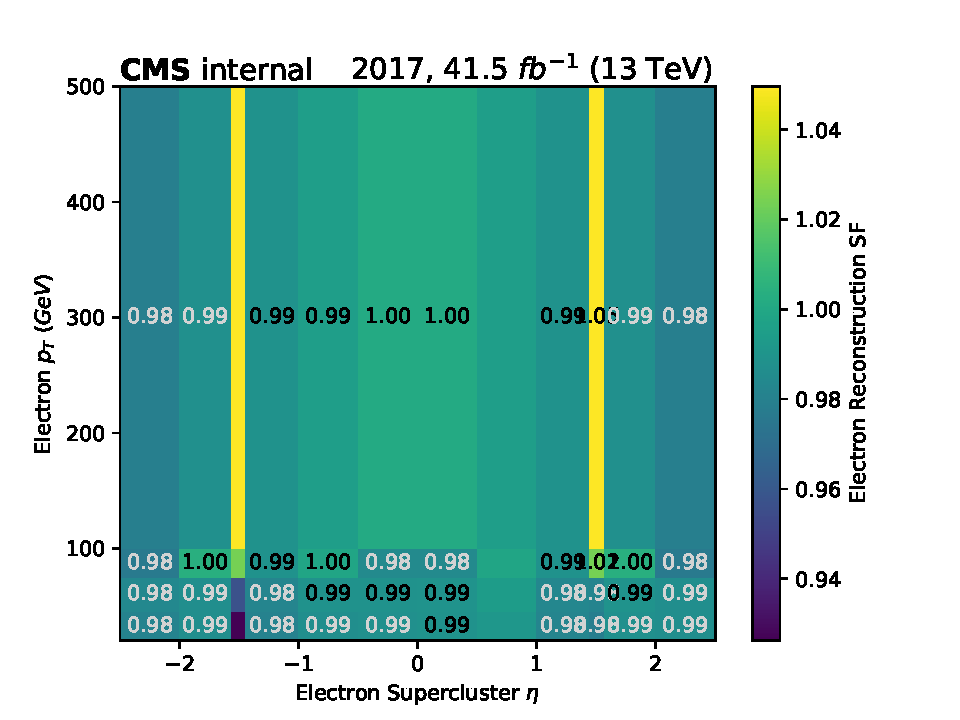
\includegraphics[width=0.49\textwidth]{ScaleFactors/Electron/electron_reco_2017.pdf}
    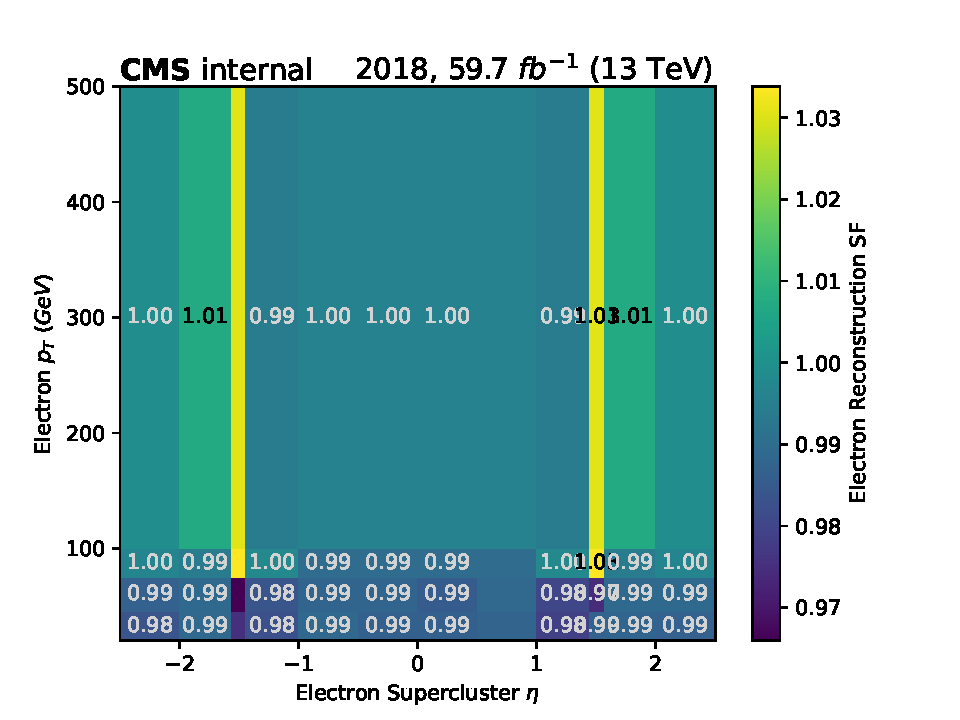
\includegraphics[width=0.49\textwidth]{ScaleFactors/Electron/electron_reco_2018.pdf} \\
    \includegraphics[width=0.49\textwidth]{ScaleFactors/Electron/electron_reco_ptbelow20_2017.pdf}
    \includegraphics[width=0.49\textwidth]{ScaleFactors/Electron/electron_reco_ptbelow20_2018.pdf}

    \caption{
      Scale factors for the reconstruction efficiency of electrons starting from a super cluster for 2017 (left) and 2018 (right), for electrons with
      $\pt > 20$ GeV (top) and $\pt < 20$ GeV (bottom).
    }
    \label{fig:sf_electron_reco}
  \end{center}
\end{figure}

\begin{figure}[ht!]
  \begin{center}
    \includegraphics[width=0.45\textwidth]{ScaleFactors/Electron/electron_id_tight_2017.pdf}
    \includegraphics[width=0.45\textwidth]{ScaleFactors/Electron/electron_id_veto_2017.pdf} \\
    \includegraphics[width=0.45\textwidth]{ScaleFactors/Electron/electron_id_tight_2018.pdf}
    \includegraphics[width=0.45\textwidth]{ScaleFactors/Electron/electron_id_veto_2018.pdf}
    \caption{
      Scale factors for the identification efficiency of tight (left) and veto (right) electrons are shown for 2017 (top) and
      2018 (bottom). The scale factors are provided in bins of electron $\pt$ and $\eta$.
    }
    \label{fig:sf_electron_id}
  \end{center}
\end{figure}

\begin{figure}[ht!]
  \begin{center}
    \includegraphics[width=0.49\textwidth]{ScaleFactors/Muon/NUM_TightID_DEN_TrackerMuons_abseta_pt_2017.pdf}
    \includegraphics[width=0.49\textwidth]{ScaleFactors/Muon/NUM_LooseID_DEN_TrackerMuons_abseta_pt_2017.pdf} \\
    \includegraphics[width=0.49\textwidth]{ScaleFactors/Muon/NUM_TightID_DEN_TrackerMuons_abseta_pt_2018.pdf}
    \includegraphics[width=0.49\textwidth]{ScaleFactors/Muon/NUM_LooseID_DEN_TrackerMuons_abseta_pt_2018.pdf}
    \caption{
      Scale factors for tight (left) and veto (right) muon identification are shown for 2017 (top) and
      2018 (bottom). The scale factors are provided in bins of muon $\pt$ and $\eta$.
    }
    \label{fig:sf_muon_id}
  \end{center}
\end{figure}

\begin{figure}[ht!]
    \begin{center}
        \includegraphics[width=0.49\textwidth]{ScaleFactors/Muon/NUM_TightRelIso_DEN_TightIDandIPCut_abseta_pt_2017.pdf}
        \includegraphics[width=0.49\textwidth]{ScaleFactors/Muon/NUM_LooseRelIso_DEN_LooseID_abseta_pt_2017.pdf} \\
        \includegraphics[width=0.49\textwidth]{ScaleFactors/Muon/NUM_TightRelIso_DEN_TightIDandIPCut_abseta_pt_2018.pdf}
        \includegraphics[width=0.49\textwidth]{ScaleFactors/Muon/NUM_LooseRelIso_DEN_LooseID_abseta_pt_2018.pdf}
        \caption{
            Scale factors for tight (left) and veto (right) muon isolation are shown for 2017 (top) and
            2018 (bottom). The scale factors are provided in bins of muon $\pt$ and $\eta$.
        }
      \label{fig:sf_muon_iso}
    \end{center}
\end{figure}

\clearpage

\subsection{Lepton veto efficiency reweighting}

To reduce contribution from $W(\ell \nu)+$ jet(s) events in the analysis signal region (SR), 
events are rejected if they contain any
identified charged lepton. However, due to finite efficiencies of the
reconstruction and identification of these candidates, $W(\ell \nu)+$ jet(s)
events still contribute significantly. Furthermore, the differences in veto efficiency between data and MC
need to be taken into account. For these purposes, the ``veto-weight'' method is used.
In this method, simulated events in the SR are allocated a veto weight instead of
being removed completely if they have charged lepton(s) in the final state. Such events with
identified leptons can enter the SR with a veto weight dependent on the identification, isolation and reconstruction 
efficiency scale factors for the identified objects
in the event. The veto weight $\omega$ is calculated as:

\begin{equation}
    \omega = \prod_{i \ \epsilon \ leptons} (1-SF_{i}) 
\end{equation}

where the product above runs over all identified veto leptons in the event (i.e. electrons, muons and taus).
$SF_{i}$ represents the total scale factor for the lepton $i$, which is the product of identification and isolation
scale factors as described in Sec.~\ref{subsec:lepton_id_reweighting}. It can be observed that this method is equivalent
to the ordinary method with hard-veto on events with leptons, as $SF \approx 1$ for events with well identified leptons,
making the event weight, $\omega \approx 0$, hence suppressing the contribution of the event in the SR.
Comparing the simulated event yields with hard
lepton veto applied (instead of lepton veto weights), it is observed that the lepton veto weights in the signal region
introduces a small correction $\ll 1\%$.

The uncertainty on these veto weights are computed by varying the veto weights within their uncertainties and
propagating the variation into the $\mjj$ distribution in the SR. Since the lepton kinematics are not largely
correlated with the kinematics of two outgoing VBF jets, the uncertainties are observed to be flat as a function
of $\mjj$.

% In Fig.~\ref{fig:sr_veto_weights}, the impact of the veto weight
% corrections (compared to the hard lepton veto) on the $\Wlvjets$ process in the VBF signal region, 
% and the uncertainty on the veto weights are shown. It can be observed that the correction
% coming from the veto weights is typically small ($\ll 1\%$), and the uncertainties on the veto weights are small
% and uncorrelated with the invariant mass of two VBF jets, $\mjj$.

% \begin{figure}[ht!]
%   \begin{center}
%     \includegraphics[width=0.45\textwidth]{ScaleFactors/VetoWeights/tau_vetow_variations_2017.pdf}
%     \includegraphics[width=0.45\textwidth]{ScaleFactors/VetoWeights/tau_vetow_variations_2018.pdf} \\
%     \includegraphics[width=0.45\textwidth]{ScaleFactors/VetoWeights/ele_vetow_variations_2017.pdf}
%     \includegraphics[width=0.45\textwidth]{ScaleFactors/VetoWeights/ele_vetow_variations_2018.pdf} \\
%     \includegraphics[width=0.45\textwidth]{ScaleFactors/VetoWeights/muon_vetow_variations_2017.pdf}
%     \includegraphics[width=0.45\textwidth]{ScaleFactors/VetoWeights/muon_vetow_variations_2018.pdf}
%     \caption{
%       The impact of the veto weight corrections on $\Wlvjets$ process in the signal region. The correction with the nominal
%       lepton veto weight and the uncertainties of the veto weight are shown, and the event yield ratio with the hard lepton veto
%       case is plotted. The top row corresponds to the tau veto, middle row to electron veto, and last row corresponds to
%       muon veto. Left and right columns represent 2017 and 2018 datasets, respectively. 
%     }
%     \label{fig:sr_veto_weights}
%   \end{center}
% \end{figure}

% \subsection{Efficiency reweighting for b-jet vetos}

% \emph{TODO: Fill this section.}

\subsection{Reweighting For HF Noise Cuts}
\label{subsec:hf_weighting}

As will be explained in Sec.~\ref{subsec:hfnoise}, several noise-cleaning cuts are implemented to reduce the contribution 
from mis-reconstruction of forward jets,
reconstructed in the Forward HCAL (HF) detector (i.e. $|\eta| > 3.0$). To account for the difference in the impact of these cuts in
data and MC, a per-jet scale factor is applied to the events in MC. These scale factors are derived by calculating the efficiency 
of these cuts on $\Zmmjets$ and $\gamma$ + jets events in data and MC, as a function of jet $\pt$ and $\eta$, and taking 
the ratio of those two efficiencies. 

The HF noise scale factors are applied for each HF jet in the event which would be taken into account for the HF cuts (i.e. $\pt > 100$ GeV 
and $\Delta\phi(j,\ptmiss) > 2.5$), as a function of $\pt$ and $\eta$ of the jet. The event weight is calculated by multiplying the individual jet weights:

\begin{equation}
    \omega_{event} = \prod_{jet \in HF} \omega_{jet} (\pt, \eta)
\end{equation}

where the product runs over each jet with $\pt > 100$ GeV and $\Delta\phi(j,\ptmiss) > 2.5$\footnote{These cuts are required
to be compatible with the application of HF cuts described in Sec.~\ref{subsec:hfnoise}. $\Delta\phi > 2.5$ requirement on
the jets being considered is utilized to pick jets that are reconstructed back-to-back (i.e. high $\Delta\phi$) with the missing
transverse momentum}.
The per-jet scale factors $\omega_{jet}$ are shown in Fig.~\ref{fig:hf_scale_factors} for 2017 and 2018, together with their statistical uncertainties. 
For the statistically limited phase space of very high $\pt$ and $\eta$ (where the scale factor is measured to be $0$), 
the scale factor in the closest $[ \pt, \eta ]$ bin is applied to the HF jet.

\begin{figure}[ht!]
    \begin{center}
        \includegraphics[width=0.49\textwidth]{ScaleFactors/HFCuts/hf_sf_2017.pdf}
        \includegraphics[width=0.49\textwidth]{ScaleFactors/HFCuts/hf_sf_2018.pdf}
        \caption{
            HF scale factors and their statistical uncertainties as a function of jet $\pt$ and $\eta$, for 2017 (left) and 2018 (right). 
            For the phase space with statistical limitations (i.e. $SF=0$), the scale factor in the closest $[ \pt, \eta ]$ bin is applied to the HF jet.
          }
        \label{fig:hf_scale_factors}
    \end{center}
\end{figure}

\clearpage

\subsection{Reweighting for ECAL pre-firing}
\label{subsec:prefiring_weighting}

Prefiring is a problem with the 2017 dataset that results from L1 trigger primitives
in the ECAL endcap being incorrectly assigned to an earlier bunch crossing because
of a timing issue. In most cases, the event to which the trigger primitives are now assigned to
fail to pass the HLT selection and is discarded. This makes the event for which the trigger
primitives were originally belonged to be discarded as well, which results in a loss of trigger
efficiency. A solution has been developed by parametrizing
the probability of a jet or photon in the event causing prefiring in terms of their
$\pt$ and $\eta$. In this analysis, the prefiring weights are applied based on the parametrization
provided by the JME POG \cite{CMS:PrefiringTwiki}, and a central implementation provided in the
NanoAOD-tools software is used \cite{CMS:PrefiringNanoAODTools}. In this implementation, a per-event
prefiring weight is computed as:

\begin{equation}
    \omega = 1 - P(prefiring) = \prod_{i=photons,jets} (1 - \epsilon_{i}^{pref}(\pt, \eta))
\end{equation}

where $\epsilon_{i}^{pref}$ is the prefiring probability caused by a single photon or a jet, and the product
runs over the photons and jets reconstructed in the event.
The $\mjj$ distributions with the nominal prefiring weight applied to simulation, together with the
up and down variations of the prefiring weight are shown in Figs.~\ref{fig:prefiring_1} and \ref{fig:prefiring_2}.
It can be observed that the uncertainty due to the prefiring weight increases with higher $\mjj$. It can be argued
that this is an expected effect because of the origins of the prefiring problem, which is much more sizable for jets
in the ECAL endcap region, $2.5 < |\eta| < 3.0$. Therefore, events with at least one forward jet is much likely to
get impacted by prefiring. Since $\mjj$ is correlated with $\detajj$ (i.e. the $\eta$ separation between the two
VBF jets), events with higher $\mjj$ are also more impacted, and hence the relevant uncertainty is more pronounced
at high $\mjj$. 

\begin{figure}[htbp]
  \centering
    \includegraphics[width=0.49\textwidth]{ScaleFactors/Prefire/cr_1e_vbf.pdf}
    \includegraphics[width=0.49\textwidth]{ScaleFactors/Prefire/cr_1m_vbf.pdf} \\
    \includegraphics[width=0.49\textwidth]{ScaleFactors/Prefire/cr_2e_vbf.pdf}
    \includegraphics[width=0.49\textwidth]{ScaleFactors/Prefire/cr_2m_vbf.pdf}
    \caption{The $\mjj$ distributions with the nominal prefiring weights and its variations
    are shown for $\Wjets$ simulation in single lepton CRs (top), and $\Zjets$ simulation in
    double lepton CRs (bottom).}
    \label{fig:prefiring_1}
\end{figure}

\begin{figure}[htbp]
  \centering
    \includegraphics[width=0.49\textwidth]{ScaleFactors/Prefire/cr_g_vbf.pdf}
    \includegraphics[width=0.49\textwidth]{ScaleFactors/Prefire/sr_vbf_qcd_wlv.pdf} \\
    \includegraphics[width=0.49\textwidth]{ScaleFactors/Prefire/sr_vbf_qcd_zvv.pdf}
    \includegraphics[width=0.49\textwidth]{ScaleFactors/Prefire/sr_vbf_vbfhinv.pdf}
    \caption{The $\mjj$ distributions with the nominal prefiring weights and its variations
    are shown for $\gamma$ + jets simulation in the photon CR (top left), $W(\ell\nu)$ + jets (top right),
    $Z(\nu\nu)$ + jets (bottom left) and VBF $\hinv$ (bottom right) in the signal region.}
    \label{fig:prefiring_2}
\end{figure}

\subsection{Higher-order reweighting}
\label{sec:nlo}

As will be detailed in Sec.~\ref{subsec:likelihood_fit}, this analysis uses the ratios of $\Vjets$ distributions in signal and control regions 
to constrain the final background estimate for $\Zvvjets$ and $\Wlvjets$ processes. 
As signal and control regions both have large statistical power, precise predictions of these ratios are necessary. 
To achieve this goal, next-to-leading-order (NLO) in QCD simulation samples are used for $\Wlvjets$ and $\Zlljets$ backgrounds, 
and corrected with higher-order EWK corrections. 
To model the $\gamma$ + jets background in photon control region, leading-order (LO) in QCD simulation samples are used instead,
which are then reweighted using higher-order QCD and EWK corrections. 
These corrections are described in more detail in the following subsections. A concise overview of which corrections are applied to 
which processes is given in Tab.~\ref{tab:higher_order_summary}.

\begin{table}[ht!]
    \centering
    \small
    \def\arraystretch{1.5}
    \caption{Summary of higher-order corrections applied to simulated samples. For each boson production process, 
      separate samples and corrections are available for the EWK and QCD production modes. ``MC order'' reflects the 
      perturbative order used in the generation of the simulation sample, while the further columns represent corrections 
      applied on a per-event level in the analysis process.}
    \begin{tabular}{c c c c c c}
        \textbf{Boson} & \textbf{Production mode}  & \textbf{MC order} & \textbf{NLO QCD}  & \textbf{NLO EWK} \\\hline\hline
    \multirow{2}{*}{Z} & QCD & NLO & --         & \checkmark \\
                       & EWK & LO  & \checkmark & -- \\\hline
    \multirow{2}{*}{W} & QCD & NLO & --         & \checkmark \\
                       & EWK & LO & \checkmark & -- \\\hline
    \multirow{2}{*}{$\gamma$} & QCD & LO &  \checkmark & \checkmark \\
    & EWK & LO & -- & -- \\\hline\hline

    \end{tabular}

    \label{tab:higher_order_summary}
\end{table}

\subsubsection{Generator-level boson construction}
All theory-based corrections of the $\Wlvjets$, $\Zlljets$, and $\gamma$ + jets backgrounds are parametrized as a function of the 
generator-level transverse momentum of the respective boson, $\ptv$. For $\Wlvjets$ and $\Zlljets$ events, this quantity is calculated as follows:

\begin{enumerate}
  \item If a boson is found in generator-level collection with \texttt{status = 62}, it's $\ptv$ is taken as the generator level $\ptv$.
  (If multiple such entries are found, highest $\ptv$ is chosen.)
  \item In the rare cases where the boson is not found in the generator-level collection, then the boson is defined as the four-vector sum of the selected leptons.
  Leptons are selected as described in the next two steps:
  % \item If there are dressed electrons or muons (taken from the \texttt{GenDressedLepton} collection) that are not coming from a tau decay, these leptons are selected
  % to compute $\ptv$.
  % \item If the dressed electrons or muons are found to be coming from a tau decay, or if there are no dressed leptons in the event, the generator-level taus 
  % are chosen to compute $\ptv$.
  \item If there are electrons or muons that are not coming from a tau decay, these leptons are selected to compute $\ptv$.
  \item If the electrons or muons are found to be coming from a tau decay, or if there are no leptons in the event, the generator-level taus 
  are chosen to compute $\ptv$.
\end{enumerate}

For $\gamma$ + jets events, the photon at generator-level is selected by requiring the following:
\begin{itemize}
    \item Photon needs to have \textit{status = 1}, indicating that it is a final state particle (i.e. a particle that is not decayed further by the generator). 
    \item Photon needs to have a prompt status flag. 
    \item $|\eta|<1.46$, so that the photon is in the barrel region. 
\end{itemize}

If there are multiple such photons, the one with highest $\pt$ is selected.

\subsubsection{Photon scale factors}

The photon scale factors are derived with a two-dimensional dependence on generator-level $\ptv$ and $\mjj$, and are shown for the MTR category in 
Fig.~\ref{fig:theory_sf_qcd_nlo_2d-photon}. These scale factors are applied to $\gamma$ + jets events as a NLO correction, and the correction depends
on the kinematics of the event.

\begin{figure}[ht!]
    \begin{center}
        \includegraphics[width=0.49\textwidth]{ScaleFactors/NLO/2d_gjets_gen_vpt_vbf_stat1.pdf}
        \caption{
            LO-to-NLO theory scale factors binned in the generator-level boson $\pt$ and $\mjj$, shown photon production.
            The k factors are derived within the generator-level VBF selection described in the text.
            The uncertainties quoted in each bin are the statistical uncertainties due to the finite size of the simulated samples.
          }
      \label{fig:theory_sf_qcd_nlo_2d-photon}
    \end{center}
\end{figure}

\subsubsection{EWK NLO corrections to QCD V processes}

Scale factors corresponding to NLO EWK corrections are obtained from Ref.~\cite{DMTheory} and applied as a function of the generator-level boson $\pt$
to each event. The scale factors are shown in Fig.~\ref{fig:theory_sf_ew_nlo}.

\begin{figure}[ht!]
    \begin{center}
        \includegraphics[width=0.49\textwidth]{ScaleFactors/NLO/nlo_ewk.pdf}
        \caption{
            EWK NLO scale factors for DY, W and photon production as a function of \ptv.
          }
      \label{fig:theory_sf_ew_nlo}
    \end{center}
\end{figure}

\subsubsection{QCD NLO corrections to EWK V processes}

The QCD NLO corrections to VBF $\Wjets$ and $\Zjets$ production have been calculated in Ref.~\cite{AN-2017-267} using the VBF@NLO program. 
They are parametrized in $\ptv$ and $\mjj$ and are shown in Fig.~\ref{fig:theory_sf_qcd_nlo_for_ewk}.

\begin{figure}[ht!]
    \begin{center}
        \includegraphics[width=0.49\textwidth]{ScaleFactors/NLO/nlo_qcd_for_ewk_dy.pdf}
        \includegraphics[width=0.49\textwidth]{ScaleFactors/NLO/nlo_qcd_for_ewk_w.pdf}
        \caption{
            QCD NLO scale factors for EWK DY, W production of $\ptv$ and $\mjj$.
          }
      \label{fig:theory_sf_qcd_nlo_for_ewk}
    \end{center}
\end{figure}

\clearpage

\subsubsection{NLO EWK Corrections on VBF Signal}
\label{subsubsec:vbf_nlo_ewk}

Next to leading order (NLO) EWK corrections on VBF signal are computed using the HAWK generator~\cite{HAWKGenerator}. 
The NLO corrections are computed in the VBF phase space, where events are selected based on the kinematics of the two final state VBF jets.
These kinematic selections are described in Sec.~\ref{sec:event_selection}.
The correction is calculated as a function of the $\pt$ of the Higgs boson, and is parametrized using the following fit function:

\begin{equation}
    \epsilon_{EWK}(p_T^{H}) = (1 - 0.000372 * p_T^{H} - 0.0304) / 0.95
\end{equation}

For each event in the VBF signal sample, this correction is applied based on the $\pt$ of the Higgs boson found in the generator-level collection.
\section{Data-quality issues}
\label{sec:dataquality}

\subsection{Forward HCAL (HF) Noise}
\label{subsec:hfnoise}

The forward HCAL (HF) detector covers the most-forward rapidity range of HCAL ($3 < |\eta| < 5$), as described in
Sec.~\ref{subsec:hcal}. Due to its very forward location and close proximity to the beam pipe, 
HF detector operates in a much harsher radiation environment. 
It should also be noted that the tracking detector, covering $|\eta| < 2.5$ range, does not extend to this high rapidity
phase space. Combination of these different factors makes it harder to reconstruct and cluster hadronic jets, 
and measure their energies accurately at the HF detector. Therefore, there
is a sizable probability that the $\pt$ of a jet reconstructed at high $|\eta|$ being highly mismeasured.
Such mismeasurements can lead to spurious $\ptmiss$ in QCD multijet events (e.g. $q\bar{q} \rightarrow q\bar{q}$),
due to $\pt$ of one of the final state jets being severely mismeasured. It should be noted that while the probability
of such severe mismeasurement is relatively small, the very large cross section of QCD multijet processes in a p-p collider
compensates for this, and the number of events with spurious $\ptmiss$ cannot be ignored.
This becomes problematic for analyses that target $\ptmiss$ (such as analyses targeting $\hinv$ signature), 
since mismeasured QCD multijet events can pass
the high $\ptmiss$ requirement imposed on the analysis signal region. Hence, this effect needs to taken into account. 

It was observed that jets resulting from such mismeasurement present a distinguishable shape with respect to well-identified jets: 
Their shower shape is spread in $\eta$ and narrow in $\phi$. Shower shape variables of HF jets ($\sieie$, $\sipip$, HF central strip size) 
have therefore been introduced and added to the event content in the input datasets. 
$\sieie$ represents the shower width of the HF jet in $\eta$ direction, and similarly, $\sipip$ represents the shower width in $\phi$ direction. 
Their definitions can be found below:

\begin{equation}
    \begin{split}
        \sieie &= \sqrt{\frac{ \sum_{i} \Delta\eta(i, jet)^2 \omega_i }{ \sum_{i} \omega_i }} \\
        \sipip &= \sqrt{\frac{ \sum_{i} \Delta\phi(i, jet)^2 \omega_i }{ \sum_{i} \omega_i }}
    \end{split}
    \label{eq:sieie_sipip}
\end{equation}

In Eq.~\ref{eq:sieie_sipip}, the sums run over all PF candidates with $\pt > 3$ GeV, and 
$\omega_i$ is the weight applied to PF candidate $i$ within the jet, which is computed as follows:

\begin{equation}
    \omega_i = \frac{p_T^i - p_T^{\text{PU offset}}}{\sum_{i} p_T^{i} - p_T^{\text{PU offset}} }
    \label{eq:omega_def}
\end{equation}

In Eq.~\ref{eq:omega_def}, $p_T^{\text{PU offset}}$ refers to the offset correction on the $\pt$ of the particle 
due to pileup (PU). It is defined as follows:

\begin{equation}
    p_T^{\text{PU offset}} = \frac{\text{jet L1 offset / gen vtx}}{\pi \times 0.4^2} \times \frac{N_{\text{reco vertices}}}{\epsilon^{reco}(\text{PU vtx})} \times S_{\text{HF tower}}
\end{equation}

The other distinguishing variable, HF central strip size ($\hfcss$), is computed as follows: 
$N_{cands}$ with $\pt > 10$ GeV \& $|\Delta\phi(cand,jet)| < 0.05$. It is a measure of the number of
highly energetic particles reconstructed close to the jet centroid (i.e. $|\Delta\phi(cand,jet)| < 0.05$).
In the event of spurious large energy deposits from a jet, one can expect larger number of energetic particles
being reconstructed closer to the jet centroid, as a result of those energy deposits.

These variables are used to define a series of cuts rejecting most of the HF-related noise, while keeping a high efficiency on well-identified jets. 
The efficiency of the cuts on physics jets in data and simulation is measured and their ratio is used to correct the simulation.
This procedure is described in Sec.~\ref{subsec:hf_weighting}. After the HF noise cuts are applied, the residual noise in the signal region is estimated using a data driven technique.
The study and the definition of the HF noise cuts, and the residual HF noise estimation are discussed in the subsections below. 

\subsubsection{Definition of HF Noise Cuts}

In order to study the discriminating power of these variables directly in data, two regions enriched in ``physics'' jets and ``noise'' jets are defined. ``Physics'' jets
refer to HF jets that are recoiling against a well-reconstructed physics object (in this study, a photon), and ``noise'' jets 
refer to HF jets that recoil against no visible physics object, hence creating $\ptmiss$ in the event. The region where the ``physics'' jets are tagged
is termed as the physics-enriched region, and the region where the ``noise'' jets are tagged is termed as the noise-enriched region.

The physics-enriched region consists of events where a HF jet recoils against a photon. 
Jet and photon being back-to-back is ensured by a series of cuts on $\Delta\phi(\gamma, jet)$,
ratio of transverse momenta of the photon and the jet, and also the requirement of low $\ptmiss$ in the event. The selections are listed below: 

\begin{itemize}
    \item Exactly one well identified photon (tight identification, as discussed in Sec.~\ref{subsec:photons})
    \item Events passing a single photon trigger requiring $p_T^{\gamma} > 110$ GeV
    \item $\Delta\phi(\gamma, jet) > 2.7$
    \item $0.5 < \frac{p_T(\gamma)}{p_T(jet)} < 1.5$
    \item $\ptmiss < 50$ GeV
\end{itemize}

The noise-enriched region includes events with exactly one high $\pt$ HF jet and high $\ptmiss$.
The aim here is to collect events with a mis-measured HF jet, such that it has very high $\pt$, but there is no other high $\pt$ physics object in the event,
giving rise to $\ptmiss$ in the event.
The complete requirements for this region are listed below:

\begin{itemize}
    \item Events passing the MET trigger described in Sec.~\ref{subsubsec:met_trigger_eff}, requiring $\ptmiss > 120$ GeV and $\htmiss > 120$ GeV
    (as reconstructed by the trigger algorithm). 
    \item $\ptmiss > 100$ GeV
    \item Exactly one HF jet with $\pt > 100$ GeV
    \item No extra jet with $\pt > 30$ GeV
    \item No lepton with $\pt > 10$ GeV
\end{itemize}

The two regions outlined above are used to study the distribution of HF shower shape variables for well-identified jets, as opposed to events
containing a mis-measured (``noisy'') jet. Mainly, two sets of cuts are studied and adopted in the analysis:

\begin{itemize}
    \item Cuts on $\sieie$ and $\sipip$
    \item Cut on HF central strip size
\end{itemize}

Since the HF-related noise strongly peaks in the $3<|\eta|<3.25$ region and the size of the HF towers is $|\eta|$ dependent, 
possibly affecting the variables under study, three $|\eta|$ regions are considered. 
Two dimensional distributions of $\sipip$ vs  $\sieie$ are shown in Fig.~\ref{fig:sieie_sipip_noise_enriched} and Fig.~\ref{fig:sieie_sipip_physics_enriched},
for the noise and physics enriched regions respectively. 
From Fig.~\ref{fig:sieie_sipip_noise_enriched}, the skewness of the 2D distribution towards high $\sieie$ and low $\sipip$
can be observed, specifically for $|\eta| < 4$. This motivates the diagonal cut of $\sieie - \sipip < 0.02$, cutting away a sizable number of noisy events while
having much less impact in the physics-enriched region. 

In the noise enriched region, there are also a large number of events observed within the region defined by $\sieie < 0.02$ and $\sipip < 0.02$. 
These are thought to be interactions of halo muons in the HF detector and this region with very low $\sieie$ and $\sipip$ is therefore also vetoed. 

For jets with $|\eta| > 4$, the requirement becomes $\sieie < 0.1$ and $\sipip > 0.02$, as large numbers of noise events are observed at very low
$\sipip$ and high $\sieie$.

\begin{figure}
    \centering
    \includegraphics[width=0.45\textwidth]{HFStudy/sigmaetaetavssigmaphiphi_METenriched.pdf}
    \includegraphics[width=0.45\textwidth]{HFStudy/sigmaetaetavssigmaphiphi_METenriched_eta3p25to4.pdf}
    \includegraphics[width=0.45\textwidth]{HFStudy/sigmaetaetavssigmaphiphi_METenriched_eta4to5p2.pdf}
    \caption{Two dimensional distribution of $\sieie$ and $\sipip$ in the noise-enriched region, split by the $|\eta|$ of the jet. The first plot shows 
    $2.99 < |\eta| < 3.25$ interval, the second one shows $3.25 < |\eta| < 4$ and the last one shows $4 < |\eta| < 5.2$. The red lines on the plots indicate
    the cuts applied on these variables.}
    \label{fig:sieie_sipip_noise_enriched}
\end{figure}

\begin{figure}
    \centering
    \includegraphics[width=0.45\textwidth]{HFStudy/sigmaetaetavssigmaphiphi_photonjets.pdf}
    \includegraphics[width=0.45\textwidth]{HFStudy/sigmaetaetavssigmaphiphi_photonjets_eta3p25to4.pdf}
    \includegraphics[width=0.45\textwidth]{HFStudy/sigmaetaetavssigmaphiphi_photonjets_eta4to5p2.pdf}
    \caption{Two dimensional distribution of $\sieie$ and $\sipip$ in the physics-enriched region, split by the $|\eta|$ of the jet. The first plot shows 
    $2.99 < |\eta| < 3.25$ interval, the second one shows $3.25 < |\eta| < 4$ and the last one shows $4 < |\eta| < 5.2$. The red lines on the plots indicate
    the cuts applied on these variables.}
    \label{fig:sieie_sipip_physics_enriched}
\end{figure}

The second cut is applied on the HF central strip size ($\hfcss$) of the jet. The two-dimensional distributions of central and adjacent strip sizes for the noise enriched
region are shown in Fig.~\ref{fig:stripsize_noise_enriched}, while the same distributions in the physics enriched region are shown in Fig.~\ref{fig:stripsize_phys_enriched}.
For the jets in noise enriched region with $2.99 < |\eta| < 3.25$ (where the noise contribution is the highest), it can be observed that around $40\%$ of jets
have $\hfcss \geq 3$, while in the physics enriched region, this fraction is very small, $\mathcal{O}(1\%)$. Therefore, a cut on the $\hfcss$ variable is adopted in 
the analysis, requiring $\hfcss < 3$ for HF jets that are back to back with $\ptmiss$. 

\begin{figure}
    \centering
    \includegraphics[width=0.45\textwidth]{HFStudy/etasizecentralvsadj_METenriched.pdf}
    \includegraphics[width=0.45\textwidth]{HFStudy/etasizecentralvsadj_METenriched_eta3p25to4.pdf}
    \includegraphics[width=0.45\textwidth]{HFStudy/etasizecentralvsadj_METenriched_eta4to5p2.pdf}
    \caption{Two dimensional distribution of central and adjacent strip sizes in the noise enriched region, split by the $|\eta|$ of the jet. The first plot shows 
    $2.99 < |\eta| < 3.25$ interval, the second one shows $3.25 < |\eta| < 4$ and the last one shows $4 < |\eta| < 5.2$.}
    \label{fig:stripsize_noise_enriched}
\end{figure}

\begin{figure}
    \centering
    \includegraphics[width=0.45\textwidth]{HFStudy/etasizecentralvsadj_gammajets.pdf}
    \includegraphics[width=0.45\textwidth]{HFStudy/etasizecentralvsadj_gammajets_eta3p25to4.pdf}
    \includegraphics[width=0.45\textwidth]{HFStudy/etasizecentralvsadj_gammajets_eta4to5p2.pdf}
    \caption{Two dimensional distribution of central and adjacent strip sizes in the physics enriched region, split by the $|\eta|$ of the jet. The first plot shows 
    $2.99 < |\eta| < 3.25$ interval, the second one shows $3.25 < |\eta| < 4$ and the last one shows $4 < |\eta| < 5.2$.}
    \label{fig:stripsize_phys_enriched}
\end{figure}


In summary, the cleaning cuts applied to HF jets are:
\begin{itemize}
    \item $2.99 < |\eta| < 4.0$: $\sieie - \sipip < 0.02$ condition is required. In addition, the corner region, defined as $\sieie < 0.02 \ \& \ \sipip < 0.02$,
    is also removed from the analysis.
    \item $|\eta| > 4.0$: $\sieie < 0.1 \ \& \ \sipip > 0.2$ condition is required.
    \item $|\eta| > 2.99$: $\hfcss < 3$ is required.
\end{itemize}

They are applied to all jets with $\pt > 100$ GeV and $|\eta| > 2.99$ that are back-to-back with $\ptmiss$
(i.e. $\Delta\phi(jet,\ptmiss) > 2.5$). If any such jet fails the cuts, the event is rejected. 


\subsubsection{Residual HF Noise Estimation}
\label{subsubsec:hf_noise_est}

In addition to the HF cleaning cuts explained in the previous subsection,
a noise estimation is done to estimate the leftover noise contribution in  
the analysis signal region. For the noise estimation, a new control region is defined
in which the HF shape cuts are inverted. Other than the HF shape cuts,
the same cuts are required in this control region as in the VBF signal region, which are
discussed in Sec.~\ref{subsec:sr_vbf_selection}. For the remainder of this text, this control
region will be referred to as HF control region.

With the addition of this HF control region (CR), the estimation is done in three steps.
First, data and MC yields in this CR are computed ($N_{data}$, $N_{MC}$). The excess amount of data over MC 
in this control region gives the number of excess events in data with HF noise, not modeled by the 
simulation: $N_{noise}^{CR} = N_{data} - N_{MC}$. 
Finally, the noise estimate in analysis signal region is calculated from $N_{noise}^{CR}$ by using $[\pt, \eta]$ dependent transfer factors,
defined as the relative probability for a noise event to pass the HF shape cuts, relative to failing them.
This probability is derived from events in a noise-enriched region, where the probability of a jet in such an event
to pass the HF cuts can be computed as a function of its pseudorapidity and transverse momentum, $\hfprobpass[p_{T}, \eta]$.
Using these probabilities, the transfer factor $R_{jet}$ for a single jet can be then written as:

\begin{equation}
    R_{jet} (p_T, \eta) = \frac{\hfprobpass}{\hfprobfail} (p_T, \eta) = \frac{\hfprobpass}{1 - \hfprobpass} (p_T, \eta)
\end{equation}

For a given event, the total transfer factor (taking all HF jets into account in the event) can be then computed as

\begin{equation}
    R_{event} = \prod_{jet} R_{jet} (p_T, \eta)
\end{equation}

where the product runs over the jets in the event with $p_T > 100$ GeV and $|eta| > 2.99$ (i.e. HF jets). If there are no
jets in the event that satisfy this criteria, $R_{event}$ is defined to be $0$, signifying the fact that there will be no contribution
to the signal region noise estimate template from this event. If there is such a jet however, $R_{event} \neq 0$, hence signifying
a non-zero contribution to the noise estimation in the signal region.

In this way, the contribution of a single event in the noise-enriched CR to the HF noise template in the signal region can be written as

\begin{equation}
    N_{noise}^{SR} = R_{event} \times (N_{data}^{CR} - N_{MC}^{CR})
    \label{eq:hf_noise_calc_single_event}
\end{equation}

Eq.~\ref{eq:hf_noise_calc_single_event} shows the contribution from a single event in the HF control region.
As the final step, summing up the contributions from all events in the HF control region gives the full $\mjj$ 
noise estimate template for the HF noise, which are shown in Fig.~\ref{fig:hf_estimation_mtr}.
Plots on the left column show the data and total MC
yields in the HF control region, each event being already scaled by the transfer factor 
$R_{event}$ as defined above. 
Plots on the right column show the resulting HF noise estimation in the analysis
signal region, which correspond to the difference of data and MC yields in the left-hand side plots.
Plots on the top show the results with 2017 data, and plots on the bottom show results with 2018 data.

\begin{figure}[h!]
    \centering
        \includegraphics[width=0.49\textwidth]{HFStudy/NoiseEstimation/cr_vbf_qcd_mjj_2017.pdf}
        \includegraphics[width=0.49\textwidth]{HFStudy/NoiseEstimation/qcd_estimation_mjj_2017.pdf} \\ 
        \includegraphics[width=0.49\textwidth]{HFStudy/NoiseEstimation/cr_vbf_qcd_mjj_2018.pdf}
        \includegraphics[width=0.49\textwidth]{HFStudy/NoiseEstimation/qcd_estimation_mjj_2018.pdf}
    \caption{HF noise estimate in 2017 (top) and 2018 (bottom) data. The plots on the left column show the data and total MC yields in the HF noise control region,
      where each event is scaled by a transfer factor $R_{event}$, as defined in the text. 
      Plots on the right show the resulting noise estimation in the signal region, which correspond to the difference of data and MC
      yields in the left-hand side plot.
    }
    \label{fig:hf_estimation_mtr}
\end{figure}

From Fig.~\ref{fig:hf_estimation_mtr}, it can be observed that the HF noise estimate in the signal region is mostly
flat as a function of $\mjj$, and can make a sizable contribution at higher $\mjj$ values where most of the other background
processes are suppressed.

To make sure that this noise estimation provides an accurate modeling of the data in the phase space where HF noise contribution is highest,
$3 < |\eta| < 3.25$, a closure test was performed. A subset of events in VBF signal region were picked, which have the leading jet in
the $3 < |\eta| < 3.25$ range, and the data yields are compared to the expected background yields in this region, including the HF noise estimation.
For these events, Fig.~\ref{fig:hf_noise_closure} shows the $\Delta\phi(p_{T,trk}^{miss}, \ptmiss)$ distribution, where $p_{T,trk}^{miss}$ refers to the
$\ptmiss$ computed only relying on the tracks reconstructed by the tracker. The HF noise contribution to the background estimation is expected to be 
especially significant at high $\Delta\phi$ values,
since such events have a forward jet with $|\eta|>3$, which is well outside the tracker range. Due to the presence of such jets, 
large $\Delta\phi$ between the tracker-only $\ptmiss$
and full $\ptmiss$ is expected. It should also be noted that for this high $\Delta\phi$ region, the VBF $\hinv$ signal contribution is expected to be small,
hence it would be expected that the data and background yields agree within a reasonable extent.

\begin{figure}[h!]
    \centering
    \includegraphics[width=0.7\textwidth]{HFStudy/NoiseEstimation/data_mc_eta_3_3_25_combined.pdf}
    \caption{$\Delta\phi(p_{T,trk}^{miss}, \ptmiss)$ distribution for the closure test on the HF noise estimate. Events plotted here pass the VBF signal 
    region selection, and have the leading jet in $3 < |\eta| < 3.25$ range, where the HF noise contribution is highest.
    It can be observed, especially at high $\Delta\phi(p_{T,trk}^{miss}, \ptmiss)$, the agreement between data and background yields is good
    after the residual HF noise estimation is taken into account. To account for residual differences, a $20\%$ flat uncertainty is assigned to the HF noise template.}
    \label{fig:hf_noise_closure}
\end{figure}

From Fig.~\ref{fig:hf_noise_closure}, it can be observed, especially at high $\Delta\phi(p_{T,trk}^{miss}, \ptmiss)$, the agreement between data and background yields is good
after the residual HF noise estimation is taken into account. To account for residual disagreements between data and background estimation, a $20\%$ flat uncertainty
is assigned to the HF noise template. 

\subsection{Missing HE-15/16 sectors in 2018}
\label{subsec:hem}

During a large part of data-taking in 2018, a submodule of the HCAL was not
functioning. As a result, no HCAL deposits have been recorded in the region of
$-3.0 < \eta < -1.3$ and $-1.57 < \phi < -0.87$ for the affected portion of the
recorded dataset. These missing HCAL deposits have the following consequences
for this analysis:

\begin{itemize}
    \item The jets that are affected will often be wrongly reconstructed as an electron. These mis-reconstructed
    electrons can pass the identification criteria imposed in the electron control regions, due
    to the lack of HCAL energy deposits. Therefore, such events with mis-reconstructed jets in
    this $[\eta,\phi]$ region can contaminate the electron control regions.
    \item Affected jets will not be calibrated correctly, because the energy of the reconstructed jet
    is dependent on all the HCAL deposits. Such mis-calibration will result in anomalous $\ptmiss$ in such events. 
\end{itemize}

Therefore, it was found that the analysis regions that are most impacted by this problem are the signal region and single 
electron control region. Additional requirements were imposed on these two regions to reject mis-reconstructed events arising
due to the missing HCAL deposits. The studies done to identify the impact on the analysis, and the requirements imposed are
outlined below. 

Figure~\ref{fig:HEM_motivation} shows the impact of a veto on 
events having electrons reconstructed in the impacted $[\eta,\phi]$ region. 
The alternative of "ignoring" electrons in that region, i.e. demoting them to jets 
and recalculating the leading jet pair and other relevant selection variables, 
leads to almost identical results: The source of these jets is QCD multijet events, 
hence very few of these events have another good electron to pass the selection for 
$W \rightarrow e \nu$ events. Therefore, an event veto is imposed on the single electron
control region, if the reconstructed electron is found to be within the impacted phase space.

\begin{figure}[htbp]
    \begin{center}
        \includegraphics[width=0.49\textwidth]{HEMStudy/cr_1e_vbf_no_hemveto_data_mc_electron_eta_2018.pdf}
        \includegraphics[width=0.49\textwidth]{HEMStudy/cr_1e_vbf_no_hemveto_data_mc_electron_phi_2018.pdf} \\
        \includegraphics[width=0.49\textwidth]{HEMStudy/cr_1e_vbf_data_mc_electron_eta_2018.pdf}
        \includegraphics[width=0.49\textwidth]{HEMStudy/cr_1e_vbf_data_mc_electron_phi_2018.pdf}
    \end{center}
    \caption{Effects of an electron veto in the affected detector region (single electron control region 2018). 
    Plots on the top show the $\eta$ and $\phi$ of the highest $\pt$ electron in the event
    without any veto, while plots on the bottom show the $\eta$ and $\phi$ of the electron with the veto.}
    \label{fig:HEM_motivation}
\end{figure}

The muon control regions are not affected from the missing HCAL deposits, 
thanks to the tight muon criteria imposed both in Z and W muon control regions.

The other impacted analysis region is the signal region. 
Figs.~\ref{fig:sr_2018_noHemCut_jetlead} and ~\ref{fig:sr_2018_noHemCut_met} show the distributions, in data and MC, of the leading and subleading 
jet $\phi$ and the $\phi$ of the $\ptmiss$ vector ($\phi_{\ptmiss}$), in the signal region in in 2018. 
From Figs.~\ref{fig:sr_2018_noHemCut_jetlead} and \ref{fig:sr_2018_noHemCut_met}, it can be observed that the agreement between data and MC is good 
except for the region where $-1.8 < \phi_{\ptmiss} < -0.6$. This is co-incident 
with the missing HCAL submodule. The same disagreement can be seen in the jet $\phi$ distributions, on the opposite side in $\phi$, 
which arises due to the signal selection requirement that the jets and missing energy are not aligned.
To mitigate this problem in the signal region, the following additional requirement is imposed on 2018 data:

\begin{itemize}
    \item For events in data where the run number is smaller than 319077 (i.e. before the HCAL submodule malfunctioning)
    no additional requirement is imposed, since those events are not impacted by the problem. Out of the full $59.7 \ fb^{-1}$
    of 2018 data, these events correspond to $21.1 \ fb^{-1}$ of integrated luminosity.
    \item For events in data where the run number is larger or equal to 319077, the event is discarded
    if it has $-1.8 < \phi_{\ptmiss} < -0.6$. These events correspond to a $38.6 \ fb^{-1}$ of integrated luminosity. 
\end{itemize}

The usage of run number to identify if the event is impacted by the missing HCAL submodule allows to keep $100\%$ of the data   
before the problem occurred. This effect is modeled in simulation by reweighting the set of events with $-1.8 < \phi_{\ptmiss} < -0.6$
with the fraction of luminosity without impact. This weight corresponds to $21.1 / 59.7 = 0.35$. Therefore, about $35\%$ of the events
with $-1.8 < \phi_{\ptmiss} < -0.6$ in simulation are kept in the analysis.

\begin{figure}[htbp]
    \begin{center}
        \includegraphics[width=0.49\textwidth]{HEMStudy/Leading_jet_phi.pdf}
        \includegraphics[width=0.49\textwidth]{HEMStudy/Subleading_jet_phi.pdf}
    \end{center}
    \caption{Leading (left) and subleading (right) jet $\phi$ distributions in the signal region from the 2018 dataset.
    The bands in the ratio plots represent the statistical uncertainties in the MC.}
    \label{fig:sr_2018_noHemCut_jetlead}
\end{figure}

\begin{figure}[htbp]
    \begin{center}
        \includegraphics[width=0.7\textwidth]{HEMStudy/MetNoMu_phi.pdf}
    \end{center}
    \caption{$\phi_{\ptmiss}$ distribution in the signal region from the 2018 dataset.}
    \label{fig:sr_2018_noHemCut_met}
\end{figure}

\clearpage
\section{Event selection}
\label{sec:event_selection}

% Directory with the stack plots
\newcommand\plotDir{DataMC/merged_2023-04-08_vbfhinv_full_analysis}

\subsection{Signal region}
\label{subsec:sr_vbf_selection}

Events in the VBF signal region are selected by using triggers which require
$\ptmissnomu > 120$ GeV and $\htmissnomu > 120$ GeV at HLT-level (described in Sec.~\ref{subsubsec:met_trigger_eff}). 
The $\ptmissnomu$ corresponds to the magnitude of the vector $\ptv$ 
sum of all the particles reconstructed by the trigger algorithm, 
while the $\htmissnomu$~is computed as the magnitude of the vector $\ptv$ sum of jets with $\pt > 20$ GeV and $|\eta| < 5.0$. 
The energy fraction attributed to neutral hadrons in these jets is required to be smaller than $90\%$. 
This requirement suppresses anomalous events with jets originating from detector noise. 
To be able to use the same triggers for selecting events in the muon control regions used for background prediction, 
muon candidates are not included in the $\ptmissnomu$ and $\htmissnomu$ computation. 
The trigger efficiency is measured to be $96\%$ for events passing the analysis selection for $\ptmiss > 250$ GeV and 
becomes more than $99\%$ efficient for events with $\ptmiss > 350$ GeV. 
The performance of these triggers are further discussed in Sec.~\ref{subsubsec:met_trigger_eff}.

Candidate events are required to have $\ptmiss > 250$ GeV. This requirement directly follows from the signal final state,
where a large $\ptmiss$ will be expected from the $\hinv$ decays. $250$ GeV threshold is chosen such that the trigger
algorithm is close to $100\%$ efficiency at this threshold, as mentioned in the paragraph above.
At least two AK4 jets are required in the final state, due to the two outgoing jets from the vector boson fusion (VBF) process
in the $\hinv$ signal.
The leading AK4 jet in the signal event is required to have $\pt > 80$ GeV and $|\eta| < 4.7$, and the subleading AK4 jet is 
required to have $\pt > 40$ GeV and $|\eta| < 4.7$.
Both leading jets are required to have neutral hadron fraction values of less than $80\%$ and charged hadron fraction 
values of at least $10\%$ to further reduce the possibility of noise contamination\footnote{It should be noted that
this requirement applies for the case where the jet is reconstructed within the tracker phase space, $|\eta| < 2.5$.
Outside of the tracker phase space, the charged hadron and neutral hadron classification becomes less well-defined.}. 
In addition, the analysis employs 
various event filters to reduce events with large misreconstructed \ptmiss~\cite{Sirunyan:2019kia} originating from 
non-collision backgrounds. The filters are complemented by a requirement on the relative difference between the default 
PF \ptmiss used in the analysis and the \ptmiss reconstructed just from calorimeter deposits and muons. 
In an event with genuine $\ptmiss$, one would expect the two $\ptmiss$ calculations to result in reasonably close values.
Following this constraint, the following cut is imposed on events,

\begin{equation}
    \frac{\Delta\ptmiss(\text{PF},\text{Calo})}{\ptmiss} < 0.5 \quad .
    \label{eq:dpfcalo_cut}
\end{equation}

In Eq.~\ref{eq:dpfcalo_cut}, $\Delta\ptmiss(\text{PF},\text{Calo})$ refers to the absolute difference of $\ptmiss$ values calculated
using the full event information (PF) and calorimeter information only (Calo).

For the VBF $\hinv$ signal events, two leading jets in opposite hemispheres are expected in the final state, with large dijet mass. 
Furthermore, these jets are expected to have large rapidity separation ($\detajj$) and small azimuthal separation ($\dphijj$). 
Therefore, this analysis employs several requirements on $\mjj$, $\detajj$ and $\dphijj$, which can be 
found in Table~\ref{tab:selection_mtr}.

The main background processes that mimic the VBF $\hinv$ signal final state in this search are the $\Zvvjets$ and $\Wlvjets$ processes. 
The $\Zvvjets$ process is an irreducible background and constitutes the largest background in the search, due to the fact that the decay
products of $\textrm{Z}$ boson (neutrinos) will not interact with the detector, causing genuine $\ptmiss$. 
In the case where the $\textrm{Z}$ boson production
is associated with two final state jets, the background final state mimics the signal final state. The leading order $\Zvvjets$ diagrams
are shown in Fig.~\ref{fig:zvv_bkg_feynman}. It should also be noted that the branching fraction for the $\textrm{Z} \rightarrow \nu\bar{\nu}$ decay is
not-negligible ($\approx 20\%$), making $\Zvvjets$ a large background in the VBF signal region. 

\begin{figure}[htbp!]
    \centering
    \includegraphics[width=0.45\textwidth]{QCDV2j_Feynman.pdf}
    \includegraphics[width=0.45\textwidth]{VBFV2j_Feynman.pdf}
    \caption{Feynman diagrams showing the electroweak (left) and strong (right) production of a $\textrm{Z}$ boson, which decays into
    a pair of neutrinos. Two hadronic jets are also produced in the final state, making such processes an irreducible background
    in the VBF $\hinv$ analysis.}
    \label{fig:zvv_bkg_feynman}
\end{figure}

Another important background comes from the $\Wlvjets$ process, where a $\textrm{W}$ boson is produced and decays leptonically,
together with the presence of two hadronic jets in the final state.
This is not an irreducible background however, due to the fact that rejecting events with reconstructed leptons
will significantly suppress this process. Because of this, a lepton veto is imposed in the signal region, where  
events containing one or more loose muons or electrons with $\pt >10$ GeV, or hadronically decaying $\tau$ 
leptons with $\pt>20$ GeV are rejected\footnote{To be more precise, for events in MC simulation, 
instead of directly rejecting an event due to
a lepton in the final state, a veto weight $\omega$ is applied that depends on the kinematics of final state lepton(s), where
$\omega \approx 0$ in the presence of one or more reconstructed leptons. In observed data, no such reweighting is done and
the hard-lepton-veto is still applied. Please see Sec.~\ref{subsec:veto_weight_reweighting}
for details.}. 

Events that contain a loose, isolated photon with $\pt>15$ GeV and $|\eta| < 2.5$ are also rejected. 
This helps to suppress electroweak (EWK) backgrounds in which a photon is radiated from the initial state.
To reduce the contamination from top quark backgrounds, events are 
rejected\footnote{This requirement significantly suppresses the top quark backgrounds, due to its very large branching fraction
to final states with b quarks (\textit{i.e.,} $\textrm{BR}(\textrm{t} \rightarrow \textrm{W}^{+} \textrm{b}) \approx 96\%$).} 
if they contain a b-tagged jet with $\pt > 20$ GeV and $|\eta| < 2.4$. 
These jets are identified using the DeepCSV algorithm~\cite{CMS_NOTE_2018-323,Sirunyan:2017ezt}, 
adopting the ``medium'' working point, which corresponds to correctly identifying a jet originating from a bottom quark with 
a probability of 80\% and misidentifying a jet originating from a charm quark (light-flavor jet) with a probability of 12 (2)\%.

Last source of background is the QCD multijet events, with $\ptmiss$ arising from mismeasurements of the jet momenta. 
This background is suppressed by requiring the minimum
azimuthal angle between the \ptvecmiss direction and each of the first four leading jets with $\pt > 30$ GeV
and $|\eta| < 4.7$ to be larger than 0.5 radians. The QCD multijet background where one or more of the jet(s) is forward (\textit{i.e.,} $|\eta|>3$)
is further suppressed by the application of dedicated HF cleaning cuts, described in Sec.~\ref{subsec:hfnoise}.

The selection requirements for the signal region in this analysis are summarized in Table~\ref{tab:selection_mtr}.

\begin{table*}[htb]
    \caption{Summary of the signal region selection requirements. Leading and subleading jets refer to the highest and second-highest \pt jets in the event.}
    \begin{center}
        \renewcommand{\arraystretch}{1}
        \resizebox{\textwidth}{!} {
            \begin{tabular}{l c c}
                Variable                           & Selection                       & Target background \\
                \hline
                Muon (electron) veto               & $\pt > 10$ GeV, $|\eta| < 2.4 (2.5)$  & \Zlljets,~\Wlvjets \\
                $\tau$ lepton veto                 & $\pt > 20$ GeV, $|\eta| < 2.3$        & \Zlljets,~\Wlvjets  \\
                Photon veto                        & $\pt > 15$ GeV, $|\eta| < 2.5$        & \phojets \\
                Bottom jet veto                    & DeepCSV medium $< 0.4941 / 0.4184$ (2017 / 2018) &  Top quark \\
                                                    & for all jets with $\pt > 20$ GeV, $|\eta| < 2.4$ & \\
                $\ptmiss$                          & ${>} 250$ GeV                           & QCD, top quark, \Zlljets \\
                $\Delta\phi$($\ptvecjet$,$\ptvecmiss$)   &  $ {>} 0.5$ radians               & QCD \\
                Two leading jet IDs                 & POG tight ID, CHF$>0.1$, NHF$<0.8$ & Noise \\
                HF-noise rejection                  & Cuts on HF shape variables, $\sieie, \sipip$ and HF central strip size & HF noise \\
                $\Delta\ptmiss(\text{PF},\text{Calo})$ / recoil & $<0.5$ & Noise \\
                Leading AK4 jet $\pt$ and $\eta$     & ${>} 80$ GeV and $ |\eta| < 4.7$      & All \\
                Subleading AK4 jet $\pt$ and $\eta$   & ${>} 40$ GeV and $ |\eta| < 4.7$      & All \\
                $\mjj$                               & ${>} 200$ GeV  \\       
                $\detajj$                            & ${>} 1.0$  \\
                $\dphijj$                            & ${<} 1.5$  \\
            \end{tabular}
        }
        \label{tab:selection_mtr}
    \end{center}
\end{table*}

It should be noted that the selections listed in Table.~\ref{tab:selection_mtr} refer to one of the two event selection categories in the analysis,
the MET-triggered (MTR) category. In addition to the MTR category, there is another orthogonal event selection category called the 
VBF-triggered (VTR) category \cite{VBFHinvAnalysisPaper}.
Events in this category are collected using different HLT paths that require the presence of two energetic jets in the final state, and have 
$160 < \ptmiss < 250$ GeV, hence the orthogonality to the MTR category being considered here ($\ptmiss > 250$ GeV). 
For the purposes of this thesis, the VTR category won't be discussed in detail, but the combined
results with the VTR category will be mentioned in Sec.~\ref{chapter:results}. 

Figs.~\ref{fig:SR_pre_vbfhinv_2017_mtr},~\ref{fig:SR_jets_vbfhinv_2017_mtr}, and~\ref{fig:SR_eta_vbfhinv_2017_mtr} 
show the distribution of the $\ptmiss$, $\mjj$, $\detajj$ and $\dphijj$ of the VBF jet pair (two highest-$\pt$ jets), the $\pt$ and $\eta$ distributions 
of the leading and subleading jets, and the $\eta$ distributions of the most central and most forward jets, respectively, for events
passing the VBF signal region selection.
The same distributions are shown for the 2018 samples in Figs.~\ref{fig:SR_pre_vbfhinv_2018_mtr},~\ref{fig:SR_jets_vbfhinv_2018_mtr},
and~\ref{fig:SR_eta_vbfhinv_2018_mtr}.

\begin{figure}[htbp]
    \begin{center}
        \includegraphics[width=0.49\textwidth]{\plotDir/sr_vbf/sr_vbf_data_mc_recoil_2017.pdf}
        \includegraphics[width=0.49\textwidth]{\plotDir/sr_vbf/sr_vbf_data_mc_mjj_2017.pdf} \\
        \includegraphics[width=0.49\textwidth]{\plotDir/sr_vbf/sr_vbf_data_mc_detajj_2017.pdf}
        \includegraphics[width=0.49\textwidth]{\plotDir/sr_vbf/sr_vbf_data_mc_dphijj_2017.pdf}
        
    \end{center}
    \caption{Recoil distribution, $\mjj$ distribution, $\detajj$ and $\dphijj$
    distribution in the VBF signal region, using 2017 dataset.}
    \label{fig:SR_pre_vbfhinv_2017_mtr}
\end{figure}

\begin{figure}[htbp]
    \begin{center}
        \includegraphics[width=0.49\textwidth]{\plotDir/sr_vbf/sr_vbf_data_mc_ak4_eta0_2017.pdf}
        \includegraphics[width=0.49\textwidth]{\plotDir/sr_vbf/sr_vbf_data_mc_ak4_pt0_2017.pdf} \\
        \includegraphics[width=0.49\textwidth]{\plotDir/sr_vbf/sr_vbf_data_mc_ak4_eta1_2017.pdf}
        \includegraphics[width=0.49\textwidth]{\plotDir/sr_vbf/sr_vbf_data_mc_ak4_pt1_2017.pdf}
    \end{center}
    \caption{Leading and subleading jets $\pt$ and $\eta$ in the VBF signal region, using 2017 dataset.}
    \label{fig:SR_jets_vbfhinv_2017_mtr}
\end{figure}

\begin{figure}[htbp]
    \begin{center}
        \includegraphics[width=0.49\textwidth]{\plotDir/sr_vbf/sr_vbf_data_mc_ak4_central_eta_2017.pdf}
        \includegraphics[width=0.49\textwidth]{\plotDir/sr_vbf/sr_vbf_data_mc_ak4_forward_eta_2017.pdf}
    \end{center}
    \caption{Most central (left) and most forward jets (right) $\eta$ of the VBF pair in the VBF signal region, using 2017 dataset.}
    \label{fig:SR_eta_vbfhinv_2017_mtr}
\end{figure}


% \begin{figure}[htbp]
%     \begin{center}
%         \includegraphics[width=0.49\textwidth]{\plotDir/sr_vbf/sr_vbf_data_mc_ak4_nef0_2017.pdf}
%         \includegraphics[width=0.49\textwidth]{\plotDir/sr_vbf/sr_vbf_data_mc_ak4_nef1_2017.pdf} \\
%         \includegraphics[width=0.49\textwidth]{\plotDir/sr_vbf/sr_vbf_data_mc_ak4_nhf0_2017.pdf}
%         \includegraphics[width=0.49\textwidth]{\plotDir/sr_vbf/sr_vbf_data_mc_ak4_nhf1_2017.pdf} \\
%     \end{center}
%     \caption{Neutral electromagnetic energy fractions (top) and neutral hadron energy fractions for the leading two jets in the VBF signal region,
%     using 2017 dataset.}
%     \label{fig:SR_nhf_nef_2017_mtr}
% \end{figure}

% \begin{figure}[htbp]
%     \begin{center}
%         \includegraphics[width=0.49\textwidth]{\plotDir/sr_vbf/sr_vbf_data_mc_ak4_chf0_2017.pdf}
%         \includegraphics[width=0.49\textwidth]{\plotDir/sr_vbf/sr_vbf_data_mc_ak4_chf1_2017.pdf}
%     \end{center}
%     \caption{Charged hadronic energy fractions for the leading two jets in the VBF signal region,
%     using 2017 dataset.}
%     \label{fig:SR_chf_2017_mtr}
% \end{figure}

\begin{figure}[htbp]
    \begin{center}
        \includegraphics[width=0.49\textwidth]{\plotDir/sr_vbf/sr_vbf_data_mc_recoil_2018.pdf}
        \includegraphics[width=0.49\textwidth]{\plotDir/sr_vbf/sr_vbf_data_mc_mjj_2018.pdf} \\
        \includegraphics[width=0.49\textwidth]{\plotDir/sr_vbf/sr_vbf_data_mc_detajj_2018.pdf}
        \includegraphics[width=0.49\textwidth]{\plotDir/sr_vbf/sr_vbf_data_mc_dphijj_2018.pdf}
    \end{center}
    \caption{Recoil distribution, $\mjj$ distribution, $\detajj$ and $\dphijj$
    distribution in the VBF signal region, using 2018 dataset.}
    \label{fig:SR_pre_vbfhinv_2018_mtr}
\end{figure}

\begin{figure}[htbp]
    \begin{center}
        \includegraphics[width=0.49\textwidth]{\plotDir/sr_vbf/sr_vbf_data_mc_ak4_eta0_2018.pdf}
        \includegraphics[width=0.49\textwidth]{\plotDir/sr_vbf/sr_vbf_data_mc_ak4_pt0_2018.pdf} \\
        \includegraphics[width=0.49\textwidth]{\plotDir/sr_vbf/sr_vbf_data_mc_ak4_eta1_2018.pdf}
        \includegraphics[width=0.49\textwidth]{\plotDir/sr_vbf/sr_vbf_data_mc_ak4_pt1_2018.pdf}
    \end{center}
    \caption{Leading and subleading jets $\pt$ and $\eta$ in the VBF signal region, using 2018 dataset.}
    \label{fig:SR_jets_vbfhinv_2018_mtr}
\end{figure}

\begin{figure}[htbp]
    \begin{center}
        \includegraphics[width=0.49\textwidth]{\plotDir/sr_vbf/sr_vbf_data_mc_ak4_central_eta_2018.pdf}
        \includegraphics[width=0.49\textwidth]{\plotDir/sr_vbf/sr_vbf_data_mc_ak4_forward_eta_2018.pdf}
    \end{center}
    \caption{Most central (left) and most forward jets (right) $\eta$ of the VBF pair in the VBF signal region, using 2018 dataset.}
    \label{fig:SR_eta_vbfhinv_2018_mtr}
\end{figure}

% \begin{figure}[htbp]
%     \begin{center}
%         \includegraphics[width=0.49\textwidth]{\plotDir/sr_vbf/sr_vbf_data_mc_ak4_nef0_2018.pdf}
%         \includegraphics[width=0.49\textwidth]{\plotDir/sr_vbf/sr_vbf_data_mc_ak4_nef1_2018.pdf} \\
%         \includegraphics[width=0.49\textwidth]{\plotDir/sr_vbf/sr_vbf_data_mc_ak4_nhf0_2018.pdf}
%         \includegraphics[width=0.49\textwidth]{\plotDir/sr_vbf/sr_vbf_data_mc_ak4_nhf1_2018.pdf} \\
%     \end{center}
%     \caption{Neutral electromagnetic energy fractions (top) and neutral hadron energy fractions for the leading two jets in the VBF signal region,
%     using 2018 dataset.}
%     \label{fig:SR_nhf_nef_2018_mtr}
% \end{figure}


% \begin{figure}[htbp]
%     \begin{center}
%         \includegraphics[width=0.49\textwidth]{\plotDir/sr_vbf/sr_vbf_data_mc_ak4_chf0_2018.pdf}
%         \includegraphics[width=0.49\textwidth]{\plotDir/sr_vbf/sr_vbf_data_mc_ak4_chf1_2018.pdf}
%     \end{center}
%     \caption{Charged hadronic energy fractions for the leading two jets in the VBF signal region,
%     using 2018 dataset.}
%     \label{fig:SR_chf_2018_mtr}
% \end{figure}

\clearpage

\subsection{Single muon control region}
\label{sec:selection_cr_1m}

Single-muon control-region events are selected using full signal-region criteria of VBF selection with the exception of the muon veto. 
The \ptmiss requirement is replaced by an identical requirement on the hadronic recoil, which is defined as the sum of \ptvecmiss and the muon \vpt (Eq.~\ref{eq:recoil_def}), 
and thus corresponds to the \pt of the W boson.
In the single-muon control region, exactly one tightly identified, isolated muon with $\pt > 20$ GeV is required. 
No additional loose muons or electrons with $\pt > 10$ GeV are allowed in the event.

Figs.~\ref{fig:cr_1m_vbf_2017_mtr} and~\ref{fig:cr_1m_vbf_2018_mtr} show the distributions of $\mjj$, $\detajj$ for the two VBF jets,
and the $\pt$ and $\eta$ of the muon, the decay product of the $W$ boson, for 2017 and 2018 datasets respectively.

\begin{figure}[htbp]
    \begin{center}
        \includegraphics[width=0.49\textwidth]{\plotDir/cr_1m_vbf/cr_1m_vbf_data_mc_mjj_2017.pdf}
        \includegraphics[width=0.49\textwidth]{\plotDir/cr_1m_vbf/cr_1m_vbf_data_mc_detajj_2017.pdf} \\
        \includegraphics[width=0.49\textwidth]{\plotDir/cr_1m_vbf/cr_1m_vbf_data_mc_muon_pt_2017.pdf}
        \includegraphics[width=0.49\textwidth]{\plotDir/cr_1m_vbf/cr_1m_vbf_data_mc_muon_eta_2017.pdf}
    \end{center}
    \caption{Comparison between 2017 data and Monte Carlo simulation in the single muon control region. Top plots
        show the $\mjj$ and $\detajj$ distributions for the two leading AK4 jets. Bottom plots show the $\pt$ and $\eta$
        of the reconstructed muon.}
    \label{fig:cr_1m_vbf_2017_mtr}
\end{figure}

\begin{figure}[htbp]
    \begin{center}
        \includegraphics[width=0.49\textwidth]{\plotDir/cr_1m_vbf/cr_1m_vbf_data_mc_mjj_2018.pdf}
        \includegraphics[width=0.49\textwidth]{\plotDir/cr_1m_vbf/cr_1m_vbf_data_mc_detajj_2018.pdf} \\
        \includegraphics[width=0.49\textwidth]{\plotDir/cr_1m_vbf/cr_1m_vbf_data_mc_muon_pt_2018.pdf}
        \includegraphics[width=0.49\textwidth]{\plotDir/cr_1m_vbf/cr_1m_vbf_data_mc_muon_eta_2018.pdf}
    \end{center}
    \caption{Comparison between 2018 data and Monte Carlo simulation in the single muon control region. Top plots
    show the $\mjj$ and $\detajj$ distributions for the two leading AK4 jets. Bottom plots show the $\pt$ and $\eta$
    of the reconstructed muon.}
    \label{fig:cr_1m_vbf_2018_mtr}
\end{figure}

\clearpage

\subsection{Single electron control region}
\label{sec:selection_cr_1e}

Events for the single-electron control region are collected with the single-electron and photon triggers described in Sec.~\ref{subsec:trigger_eff_reweighting}.
Similar to the muon control regions, the \ptmiss requirement is replaced with an identical requirement on the hadronic recoil, which is defined as the sum of \ptvecmiss 
and the electron \vpt (Eq.~\ref{eq:recoil_def}), and thus corresponds to the \pt of the W boson.
The events in the single-electron control region are required to contain exactly one tightly identified and isolated electron with $\pt > 40$ GeV.
In addition, the contamination from QCD multijet events in this control region is suppressed by requiring $\ptmiss > 80$ GeV.

Figs.~\ref{fig:cr_1e_vbf_2017_mtr} and~\ref{fig:cr_1e_vbf_2018_mtr} show the distributions of $\mjj$, $\detajj$ for the two VBF jets,
and the $\pt$ and $\eta$ of the electron, the decay product of the $W$ boson, for 2017 and 2018 datasets respectively.

\begin{figure}[htbp]
    \begin{center}
        \includegraphics[width=0.49\textwidth]{\plotDir/cr_1e_vbf/cr_1e_vbf_data_mc_mjj_2017.pdf}
        \includegraphics[width=0.49\textwidth]{\plotDir/cr_1e_vbf/cr_1e_vbf_data_mc_detajj_2017.pdf} \\
        \includegraphics[width=0.49\textwidth]{\plotDir/cr_1e_vbf/cr_1e_vbf_data_mc_electron_pt_2017.pdf}
        \includegraphics[width=0.49\textwidth]{\plotDir/cr_1e_vbf/cr_1e_vbf_data_mc_electron_eta_2017.pdf}
    \end{center}
    \caption{Comparison between 2017 data and Monte Carlo simulation in the single electron control region. Top plots
    show the $\mjj$ and $\detajj$ distributions for the two leading AK4 jets. Bottom plots show the $\pt$ and $\eta$
    of the reconstructed electron.}
    \label{fig:cr_1e_vbf_2017_mtr}
\end{figure}

\begin{figure}[htbp]
    \begin{center}
        \includegraphics[width=0.49\textwidth]{\plotDir/cr_1e_vbf/cr_1e_vbf_data_mc_mjj_2018.pdf}
        \includegraphics[width=0.49\textwidth]{\plotDir/cr_1e_vbf/cr_1e_vbf_data_mc_detajj_2018.pdf} \\
        \includegraphics[width=0.49\textwidth]{\plotDir/cr_1e_vbf/cr_1e_vbf_data_mc_electron_pt_2018.pdf}
        \includegraphics[width=0.49\textwidth]{\plotDir/cr_1e_vbf/cr_1e_vbf_data_mc_electron_eta_2018.pdf}
    \end{center}
    \caption{Comparison between 2018 data and Monte Carlo simulation in the single electron control region. Top plots
    show the $\mjj$ and $\detajj$ distributions for the two leading AK4 jets. Bottom plots show the $\pt$ and $\eta$
    of the reconstructed electron.}
    \label{fig:cr_1e_vbf_2018_mtr}
\end{figure}

\clearpage

\subsection{Double muon control region}
\label{sec:selection_cr_2m}

Double-muon control region events are selected using full signal-region criteria of VBF category with the exception of the muon veto. 
In the double-muon control region, events are selected by requiring leading (subleading) muon \pt greater than 20 (10) GeV and 
an invariant mass of the two muons is required to be in the range of 60 to 120 GeV, compatible with a $\textrm{Z} \rightarrow \mu \mu$ decay. 
At least one of the two muons is required to 
pass the tight candidate definition, as defined in Sec.~\ref{subsec:muons}. 
Events are rejected if there is an additional loose muon or electron with $\pt > 10$ GeV. 
The SR \ptmiss requirement is replaced with an identical requirement on the hadronic recoil, 
which is defined as the sum of \ptvecmiss 
and the muon \vpt (Eq.~\ref{eq:recoil_def}), and thus corresponds to the distribution of the Z \pt smeared
with the $\ptmiss$ resolution of the detector.

Figs.~\ref{fig:cr_2m_vbf_2017_mtr} and~\ref{fig:cr_2m_vbf_2018_mtr} show the distributions of the recoil, $\mjj$, $\detajj$ and  
$\dphijj$ of the two leading AK4 jets for events in the double-muon control region for the VBF category 
in 2017 and 2018 datasets, respectively. Figs.~\ref{fig:cr_2m_vbf_2017_mtr_2} and~\ref{fig:cr_2m_vbf_2018_mtr_2} show the distributions 
of the leading muon \pt and $\eta$, as well as the dimuon mass and minimum $\dphi$ between 4 leading jets and recoil, for 2017 and 2018, respectively.

\begin{figure}[htbp]
    \begin{center}
        \includegraphics[width=0.49\textwidth]{\plotDir/cr_2m_vbf/cr_2m_vbf_data_mc_recoil_2017.pdf}
        \includegraphics[width=0.49\textwidth]{\plotDir/cr_2m_vbf/cr_2m_vbf_data_mc_mjj_2017.pdf} \\
        \includegraphics[width=0.49\textwidth]{\plotDir/cr_2m_vbf/cr_2m_vbf_data_mc_detajj_2017.pdf}
        \includegraphics[width=0.49\textwidth]{\plotDir/cr_2m_vbf/cr_2m_vbf_data_mc_dphijj_2017.pdf}
    \end{center}
    \caption{Comparison between 2017 data and Monte Carlo simulation in the double muon control region for
        the recoil, $\mjj$ distribution, $\detajj$ and $\dphijj$ distributions for the two leading AK4 jets.}
    \label{fig:cr_2m_vbf_2017_mtr}
\end{figure}

\begin{figure}[htbp]
    \begin{center}
        \includegraphics[width=0.49\textwidth]{\plotDir/cr_2m_vbf/cr_2m_vbf_data_mc_muon_pt0_2017.pdf}
        \includegraphics[width=0.49\textwidth]{\plotDir/cr_2m_vbf/cr_2m_vbf_data_mc_muon_eta0_2017.pdf}
        \includegraphics[width=0.49\textwidth]{\plotDir/cr_2m_vbf/cr_2m_vbf_data_mc_dimuon_mass_2017.pdf}
        \includegraphics[width=0.49\textwidth]{\plotDir/cr_2m_vbf/cr_2m_vbf_data_mc_dphijr_2017.pdf}
    \end{center}
    \caption{Comparison between 2017 data and Monte Carlo simulation in the double muon control region for
        the $\pt$ and $\eta$ of the leading muon (top), and dimuon mass and minimum $\dphi$ between 4 leading jets and recoil (bottom).}
    \label{fig:cr_2m_vbf_2017_mtr_2}
\end{figure}

\begin{figure}[htbp]
    \begin{center}
        \includegraphics[width=0.49\textwidth]{\plotDir/cr_2m_vbf/cr_2m_vbf_data_mc_recoil_2018.pdf}
        \includegraphics[width=0.49\textwidth]{\plotDir/cr_2m_vbf/cr_2m_vbf_data_mc_mjj_2018.pdf} \\
        \includegraphics[width=0.49\textwidth]{\plotDir/cr_2m_vbf/cr_2m_vbf_data_mc_detajj_2018.pdf}
        \includegraphics[width=0.49\textwidth]{\plotDir/cr_2m_vbf/cr_2m_vbf_data_mc_dphijj_2018.pdf}
    \end{center}
    \caption{Comparison between 2018 data and Monte Carlo simulation in the double muon control region for
        the recoil, $\mjj$ distribution, $\detajj$ and $\dphijj$ distributions for the two leading AK4 jets.}
    \label{fig:cr_2m_vbf_2018_mtr}
\end{figure}

\begin{figure}[htbp]
    \begin{center}
        \includegraphics[width=0.49\textwidth]{\plotDir/cr_2m_vbf/cr_2m_vbf_data_mc_muon_pt0_2018.pdf}
        \includegraphics[width=0.49\textwidth]{\plotDir/cr_2m_vbf/cr_2m_vbf_data_mc_muon_eta0_2018.pdf}
        \includegraphics[width=0.49\textwidth]{\plotDir/cr_2m_vbf/cr_2m_vbf_data_mc_dimuon_mass_2018.pdf}
        \includegraphics[width=0.49\textwidth]{\plotDir/cr_2m_vbf/cr_2m_vbf_data_mc_dphijr_2018.pdf}
    \end{center}
    \caption{Comparison between 2018 data and Monte Carlo simulation in the double muon control region for
        the $\pt$ and $\eta$ of the leading muon (top), dimuon mass and minimum $\dphi$ between 4 leading jets and recoil (bottom).}
    \label{fig:cr_2m_vbf_2018_mtr_2}
\end{figure}

\clearpage

\subsection{Double electron control region}
\label{sec:selection_cr_2e}

Events for the double-electron control region are collected with the single-electron and 
photon triggers described in Sec.~\ref{subsec:trigger_eff_reweighting}. In the offline analysis, events in the dielectron 
control region are required to contain exactly two oppositely charged electrons with leading (trailing) 
electron \pt greater than 40 (10) GeV, with at least one of the two passing the tight candidate definition, as defined in Sec.~\ref{subsec:electrons}.
Similar to the double-muon region, the invariant mass of the electron-positron pair is required to be in the range of $60$ to $120$ GeV,
thus being compatible with a $\textrm{Z} \rightarrow ee$ decay. 
The SR \ptmiss requirement is replaced with an identical requirement on the hadronic recoil, which is defined as the 
sum of \ptvecmiss and the electron \vpt (Eq.~\ref{eq:recoil_def}), and thus corresponds to the distribution of the Z \pt smeared with the \ptmiss resolution. 

Figs.~\ref{fig:cr_2e_vbf_2017_mtr} and~\ref{fig:cr_2e_vbf_2018_mtr} show the distributions of the recoil, $\mjj$, $\detajj$ and
$\dphijj$ for the two leading AK4 jets for events in the double-electron control region for the VBF category 
in 2017 and 2018 datasets, respectively. 
Figs.~\ref{fig:cr_2e_vbf_2017_mtr_2} and~\ref{fig:cr_2e_vbf_2018_mtr_2} show the distributions of the leading electron \pt and $\eta$, 
as well as the dielectron mass and minimum $\dphi$ between 4 leading jets and recoil, for 2017 and 2018, respectively.

\begin{figure}[htbp]
    \begin{center}
        \includegraphics[width=0.49\textwidth]{\plotDir/cr_2e_vbf/cr_2e_vbf_data_mc_recoil_2017.pdf}
        \includegraphics[width=0.49\textwidth]{\plotDir/cr_2e_vbf/cr_2e_vbf_data_mc_mjj_2017.pdf} \\
        \includegraphics[width=0.49\textwidth]{\plotDir/cr_2e_vbf/cr_2e_vbf_data_mc_detajj_2017.pdf}
        \includegraphics[width=0.49\textwidth]{\plotDir/cr_2e_vbf/cr_2e_vbf_data_mc_dphijj_2017.pdf}
    \end{center}
    \caption{Comparison between 2017 data and Monte Carlo simulation in the double electron control region for
        the recoil, $\mjj$ distribution, $\detajj$ and $\dphijj$ distributions for the two leading AK4 jets.}
    \label{fig:cr_2e_vbf_2017_mtr}
\end{figure}

\begin{figure}[htbp]
    \begin{center}
        \includegraphics[width=0.49\textwidth]{\plotDir/cr_2e_vbf/cr_2e_vbf_data_mc_electron_pt0_2017.pdf}
        \includegraphics[width=0.49\textwidth]{\plotDir/cr_2e_vbf/cr_2e_vbf_data_mc_electron_eta0_2017.pdf}
        \includegraphics[width=0.49\textwidth]{\plotDir/cr_2e_vbf/cr_2e_vbf_data_mc_dielectron_mass_2017.pdf}
        \includegraphics[width=0.49\textwidth]{\plotDir/cr_2e_vbf/cr_2e_vbf_data_mc_dphijr_2017.pdf}
    \end{center}
    \caption{Comparison between 2017 data and Monte Carlo simulation in the double electron control region for
        the $\pt$ and $\eta$ of the leading electron (top), dielectron mass and minimum $\dphi$ between 4 leading jets and recoil (bottom).}
    \label{fig:cr_2e_vbf_2017_mtr_2}
\end{figure}

\begin{figure}[htbp]
    \begin{center}
        \includegraphics[width=0.49\textwidth]{\plotDir/cr_2e_vbf/cr_2e_vbf_data_mc_recoil_2018.pdf}
        \includegraphics[width=0.49\textwidth]{\plotDir/cr_2e_vbf/cr_2e_vbf_data_mc_mjj_2018.pdf} \\
        \includegraphics[width=0.49\textwidth]{\plotDir/cr_2e_vbf/cr_2e_vbf_data_mc_detajj_2018.pdf}
        \includegraphics[width=0.49\textwidth]{\plotDir/cr_2e_vbf/cr_2e_vbf_data_mc_dphijj_2018.pdf}
    \end{center}
    \caption{Comparison between 2018 data and Monte Carlo simulation in the double electron control region for
        the recoil, $\mjj$ distribution, $\detajj$ and $\dphijj$ distributions for the two leading AK4 jets.}
    \label{fig:cr_2e_vbf_2018_mtr}
\end{figure}

\begin{figure}[htbp]
    \begin{center}
        \includegraphics[width=0.49\textwidth]{\plotDir/cr_2e_vbf/cr_2e_vbf_data_mc_electron_pt0_2018.pdf}
        \includegraphics[width=0.49\textwidth]{\plotDir/cr_2e_vbf/cr_2e_vbf_data_mc_electron_eta0_2018.pdf}
        \includegraphics[width=0.49\textwidth]{\plotDir/cr_2e_vbf/cr_2e_vbf_data_mc_dielectron_mass_2018.pdf}
        \includegraphics[width=0.49\textwidth]{\plotDir/cr_2e_vbf/cr_2e_vbf_data_mc_dphijr_2018.pdf}
    \end{center}
    \caption{Comparison between 2018 data and Monte Carlo simulation in the double electron control region for
        the $\pt$ and $\eta$ of the leading electron (top), dielectron mass and minimum $\dphi$ between 4 leading jets and recoil (bottom).}
    \label{fig:cr_2e_vbf_2018_mtr_2}
\end{figure}

\clearpage

\subsection{Photon control region}
\label{sec:selection_cr_g}

To further constrain the \Zvv \ background in the signal region, a photon control region is used.
At large transverse momenta, the kinematic properties of photon production become similar to those of the $\Zvv$ process, 
and can therefore be used to estimate the latter. Events for the control region are selected using a trigger requiring 
an online photon \pt of at least $200$ GeV. In the offline analysis, photons are required to be located in the barrel 
part of the detector ($|\eta|<1.4442$), have transverse momenta of at least $230$ GeV to ensure full trigger efficiency, 
and pass additional identification criteria based on the properties of the associated supercluster in the ECAL, 
as well as the isolation of the photon relative to nearby energy objects. To be considered for the control region, 
events must have exactly one such photon, with no additional photons or leptons passing the loose criteria described above. 
Jets and hadronic recoil are required to pass criteria identical to those imposed in the signal region, where the recoil 
is defined as as the vectorial sum of \ptvecmiss and the photon transverse momentum (Eq.~\ref{eq:recoil_def}).

Figs.~\ref{fig:Photon_vbfhinv_2017} and~\ref{fig:Photon_vbfhinv_2018} show the distributions of the recoil, $\mjj$, $\detajj$ and 
$\dphijj$ distributions of the two leading AK4 jets for events in the photon control region for the VBF category in the 
2017 and 2018 datasets, respectively. Similarly, Figs.~\ref{fig:Photon2_vbfhinv_2017} and~\ref{fig:Photon2_vbfhinv_2018} 
show the distributions of the photon $\pt$ and $\eta$.

\begin{figure}[htbp]
    \begin{center}
        \includegraphics[width=0.49\textwidth]{\plotDir/cr_g_vbf/cr_g_vbf_data_mc_recoil_2017.pdf}
        \includegraphics[width=0.49\textwidth]{\plotDir/cr_g_vbf/cr_g_vbf_data_mc_mjj_2017.pdf} \\
        \includegraphics[width=0.49\textwidth]{\plotDir/cr_g_vbf/cr_g_vbf_data_mc_detajj_2017.pdf}
        \includegraphics[width=0.49\textwidth]{\plotDir/cr_g_vbf/cr_g_vbf_data_mc_dphijj_2017.pdf}
    \end{center}
    \caption{Comparison between 2017 data and Monte Carlo simulation in the photon control region for
        the recoil distribution, the $\mjj$ distribution, $\detajj$ distribution and $\dphijj$ distribution
        for the two leading AK4 jets. The $\mjj$ and recoil distributions include the QCD estimate
        calculated from the photon purity measurement, as described in Sec.~\ref{subsec:photonpurity}. }
    \label{fig:Photon_vbfhinv_2017}
\end{figure}

\begin{figure}[htbp]
    \begin{center}
        \includegraphics[width=0.49\textwidth]{\plotDir/cr_g_vbf/cr_g_vbf_data_mc_photon_pt0_2017.pdf}
        \includegraphics[width=0.49\textwidth]{\plotDir/cr_g_vbf/cr_g_vbf_data_mc_photon_eta0_2017.pdf}
    \end{center}
    \caption{Comparison between 2017 data and Monte Carlo simulation in the photon control region for
        the $\pt$ and $\eta$ of the leading photon.}
    \label{fig:Photon2_vbfhinv_2017}
\end{figure}

\begin{figure}[htbp]
    \begin{center}
        \includegraphics[width=0.49\textwidth]{\plotDir/cr_g_vbf/cr_g_vbf_data_mc_recoil_2018.pdf}
        \includegraphics[width=0.49\textwidth]{\plotDir/cr_g_vbf/cr_g_vbf_data_mc_mjj_2018.pdf} \\
        \includegraphics[width=0.49\textwidth]{\plotDir/cr_g_vbf/cr_g_vbf_data_mc_detajj_2018.pdf}
        \includegraphics[width=0.49\textwidth]{\plotDir/cr_g_vbf/cr_g_vbf_data_mc_dphijj_2018.pdf}
    \end{center}
    \caption{Comparison between 2018 data and Monte Carlo simulation in the photon control region for
        the recoil distribution, the $\mjj$ distribution, $\detajj$ distribution and $\dphijj$ distribution
        for the two leading AK4 jets. The $\mjj$ and recoil distributions include the QCD estimate
        calculated from the photon purtiy measurement, as described in Sec.~\ref{subsec:photonpurity}. }
    \label{fig:Photon_vbfhinv_2018}
\end{figure}

\begin{figure}[htbp]
    \begin{center}
        \includegraphics[width=0.49\textwidth]{\plotDir/cr_g_vbf/cr_g_vbf_data_mc_photon_pt0_2018.pdf}
        \includegraphics[width=0.49\textwidth]{\plotDir/cr_g_vbf/cr_g_vbf_data_mc_photon_eta0_2018.pdf}
    \end{center}
    \caption{Comparison between 2018 data and Monte Carlo simulation in the photon control region for
        the $\pt$ and $\eta$ of the leading photon.}
    \label{fig:Photon2_vbfhinv_2018}
\end{figure}

\clearpage
\section{Signal extraction strategy}
\label{sec:signal_extraction}

% Directory with the transfer factor plots
\newcommand\tfPlotDir{TransferFactors/merged_2023-04-08_vbfhinv_full_analysis_NLO_VJets_09Apr23_thesis_v1}

The largest background contributions from \Zvvjets~and \Wlvjets~processes
are estimated using data from five mutually exclusive control regions (CR), which are described in
Sec.~\ref{sec:event_selection}. These control regions consist of:

\begin{itemize}
  \item $\Wmnjets$ region (Sec.~\ref{sec:selection_cr_1m})
  \item $\Wenjets$ region (Sec.~\ref{sec:selection_cr_1e})
  \item $\Zmmjets$ region (Sec.~\ref{sec:selection_cr_2m})
  \item $\Zeejets$ region (Sec.~\ref{sec:selection_cr_2e})
  \item $\gamma$ + jets region (Sec.~\ref{sec:selection_cr_g})
\end{itemize}

$\Vjets$ yields in the signal region is estimated by performing a simultaenous fit to the data 
in all signal and control regions, as will be explained in detail in Sec.~\ref{subsec:likelihood_fit}.

The remaining backgrounds that contribute to the total event yield in the signal region
are much smaller than those from \Zvvjets~and \Wlvjets~processes, due to the fact that they are
suppressed by kinematic cuts imposed in the VBF signal region (please see Sec.~\ref{subsec:sr_vbf_selection} for the discussion). 
These backgrounds can be summarized as the following: 

\begin{itemize}
    \item QCD multijet events, measured from data using a $\Delta\phi$ extrapolation method~\cite{VBFHinvAnalysisPaper}.
    \item Events from forward HCAL (HF) noise, measured from an orthogonal CR as explained in Sec.~\ref{subsec:hfnoise}.
    \item Top and diboson processes, which are estimated from simulation.
\end{itemize}

\subsection{Binned likelihood fit}
\label{subsec:likelihood_fit}

A binned maximum likelihood fit to the observed data is performed simultaneously across the 
signal and control regions. For each $\mjj$ bin $i$ in every region, the expected yield of $\Vjets$ events
is parametrized as a function of expected strong $\Zvvjets$ yields in the signal region, labeled as
$\kappazi$ in the following. This parametrization is done using transfer factors between different
$\Vjets$ processes, as will be explained later in this section. To scale the expected amount of VBF
$\hinv$ signal in the VBF signal region, a signal strength parameter $\mu$ is also introduced to
the fit, and left freely floating. The resulting likelihood function is shown in Eq.~\ref{eq:fit_likelihood_func}.

% A combined likelihood function is constructed representing the Poisson probability to observe the data
% in each $\mjj$ bin, given the expected background yields. This likelihood function consists of
% the product of Poisson probabilities for each $\mjj$ bin in every region (signal region and the 
% five control regions). The likelihood function is presented in Eq.~\ref{eq:fit_likelihood_func}.

% 
% Likelihood from AN
% 

% \begingroup
% \small
% \begin{align}
% \mathcal{L}(\boldsymbol{\mu}^{\Zvv}, \boldsymbol{\mu}, \boldsymbol{\theta}) = &
% \prod_{i} \mathrm{Pois}\left(d_{i} | B_{i}(\boldsymbol{\theta}) + (1+f_{i}(\boldsymbol{\theta})_{\mathrm{QCD}}) \muz_{i} + R^{EW/QCD}_{i} (1+f_{i}(\boldsymbol{\theta})_{\mathrm{EW}}) \muz_{i}+ \boldsymbol{\mu} S_{i}(\boldsymbol{\theta})\right ) \times \nonumber\\
% &\prod_{i} \mathrm{Pois} \left(d^{Z}_{i}|B^{Z}_{i}(\boldsymbol{\theta}) +\frac{\muz_{i} }{R^{Z}_{i} (\boldsymbol{\theta})_{\mathrm{QCD}}} + \frac{\muz_{i} }{R^{Z}_{i} (\boldsymbol{\theta})_{\mathrm{EW}}} \right) \times \nonumber\\
% & \prod_{i} \mathrm{Pois}\left(d^{W}_{i}|B^{W}_{i}(\boldsymbol{\theta}) +\frac{f_{i}(\boldsymbol{\theta})_{\mathrm{QCD}}\,\muz_{i}}{R^{W}_{i}(\boldsymbol{\theta})_{\mathrm{QCD}}}+\frac{f_{i}(\boldsymbol{\theta})_{\mathrm{EW}}\,\muz_{i} }{R^{W}_{i} (\boldsymbol{\theta})_{\mathrm{EW}}} \right) \times \nonumber\\
% & \prod_{i} \mathrm{Pois}\left(d^{\gamma}_{i}|B^{\gamma}_{i}(\boldsymbol{\theta}) +\frac{\muz_{i}}{R^{\gamma}_{i}(\boldsymbol{\theta})_{\mathrm{QCD}}}+\frac{\muz_{i} }{R^{\gamma}_{i} (\boldsymbol{\theta})_{\mathrm{EW}}} \right) \nonumber\\
% \end{align}
% \label{eq:fit_likelihood_func}
% \endgroup

\begin{equation}
  \label{eq:fit_likelihood_func}
  \begin{aligned}
  \mathcal{L} (\mu,\kappaz, \boldsymbol{\theta}) = & \prod_{i} \mathrm{P}\left(d_{i} \Big{|} B_{i}(\boldsymbol{\theta}) + Z_{i}(\kappazi)+W_{i}(\kappazi,\boldsymbol{\theta}) + \mu S_{i}(\boldsymbol{\theta})\right) \\
  %&\prod_{\mathrm{CR}} \left( \prod_{i} \mathrm{P} \left(d^{\mathrm{CR}}_{i} \Big{|} B^{\mathrm{CR}}_{i}(\boldsymbol{\theta}) +\frac{\kappazi }{R^{\mathrm{CR}}_{i} (\boldsymbol{\theta})_{\mathrm{Q}}} + \frac{R^{\PZ}_{i} \kappazi }{R^{\mathrm{CR}}_{i} (\boldsymbol{\theta})_{\mathrm{E}}} \right)\right) \times \prod_{j} \mathrm{P}(\theta_{j}), \\
  & \prod_{\mathrm{CR}} \left( \prod_{i} \mathrm{P} \left(d^{\mathrm{CR}}_{i} \Big{|} B^{\mathrm{CR}}_{i}(\boldsymbol{\theta}) + V_{i}^{\mathrm{CR,strong}}(\kappazi,\boldsymbol{\theta}) + V_{i}^{\mathrm{CR,VBF}}(\kappazi,\boldsymbol{\theta}) \right)\right) \\
   & \prod_{j} \mathrm{P}(\theta_{j}), \\
  Z_{i}(\kappazi) = & (1+Z^{\frac{\mathrm{VBF}}{\mathrm{strong}}}_{i}) \kappazi, \\
  W_{i}(\kappazi,\boldsymbol{\theta}) = & (f^{\mathrm{W/Z,strong}}_{i}(\boldsymbol{\theta}) + Z^{\frac{\mathrm{VBF}}{\mathrm{strong}}}_{i} f^{\mathrm{W/Z,VBF}}_{i}(\boldsymbol{\theta})) \kappazi, \\
  V_{i}^{\mathrm{CR,strong}}(\kappazi,\boldsymbol{\theta}) = & C^{\mathrm{CR,strong}}_{i}(\boldsymbol{\theta}) R^{\mathrm{CR}}_{i}(\boldsymbol{\theta}) \kappazi, \\
  V_{i}^{\mathrm{CR,VBF}}(\kappazi,\boldsymbol{\theta}) = &C^{\mathrm{CR,VBF}}_{i}(\boldsymbol{\theta}) Z^{\frac{\mathrm{VBF}}{\mathrm{strong}}}_{i} R^{\mathrm{CR}}_{i}(\boldsymbol{\theta}) \kappazi, \\
  \end{aligned}
\end{equation}

where ${\mathrm{P}(x|y) = y^{x}e^{-y}/x!}$. $d^{\mathrm{CR}}_{i}$
and $d_{i}$ are the observed number of events in each bin $i$ of
the $\mjj$ distribution in the CRs and SR, respectively. The index $i$ runs
over the $\mjj$ bins in all regions and data taking years (i.e. 2017 and 2018).

In a given bin, $\Vjets$ background yields expected in the SR are
obtained from transfer factors relating the yields in different
CRs to the yields in the SR, denoted as
$R^{\mathrm{CR}}_{i}(\boldsymbol{\theta})$. These transfer factors are 
obtained from simulation. For the single-lepton (dilepton) CRs, the factor
$R^{\mathrm{CR}}_{i}(\boldsymbol{\theta})$ refers to the ratio
of $\Wjets$ ($\Zjets$) yields from the corresponding CR to the SR. In the
photon CR, it refers to the ratio of $\phojets$ to $\Zvvjets$ yields.

In addition, transfer factors are defined between the W ($\gamma$) and
the Z processes, separately for the VBF and strong productions,
denoted as $f^{\mathrm{W/Z,proc}}_{i}(\boldsymbol{\theta})$
($f^{\gamma\mathrm{/Z,proc}}_{i}(\boldsymbol{\theta})$), with
proc denoting the production mode (strong or VBF). Lastly, a transfer factor allows the
relation of the VBF production to the strong production for $\Zvvjets$,
denoted as $Z^{\frac{\mathrm{VBF}}{\mathrm{strong}}}_{i}$. The factors
$C^{\mathrm{CR,strong}}_{i}(\boldsymbol{\theta})$ and
$C^{\mathrm{CR,VBF}}_{i}(\boldsymbol{\theta})$ are dependent on the
CR, with: $C^{(ee,\mu\mu)\mathrm{,proc}}_{i} =
1$, $C^{(e,\mu)\mathrm{,proc}}_{i} =
f^{\mathrm{W/Z,proc}}_{i}(\boldsymbol{\theta})$,
$C^{\gamma\mathrm{,proc}}_{i} =
f^{\gamma\mathrm{/Z,proc}}_{i}(\boldsymbol{\theta})$.

The contributions from subleading backgrounds in each region are
estimated directly from simulation and they are denoted by
$B^{\mathrm{CR}}_{i}(\boldsymbol{\theta})$ in the CRs, and
$B_{i}(\boldsymbol{\theta})$ in the SR. Finally, the likelihood also
includes a signal term in which $S_i$ represents the expected signal
prediction from the sum of the main Higgs production mechanisms
(\ggH, \vbf, \vh, \tth) assuming SM cross sections, while $\mu
= \sigmabr$ denotes the signal strength parameter, also left freely
floating.

Systematic uncertainties are modeled as constrained nuisance
parameters ($\boldsymbol{\theta}$), with a log-normal distribution for
those which affect the overall normalisation of a given process, and
Gaussian priors for those which directly affect the transfer factors,
indicated by $\mathrm{P}(\theta_{j})$ in Eq.~\ref{eq:fit_likelihood_func}.

% 
% Fit description from AN
% 

% The fit is performed simultaneously in the five different control regions and in the signal
% region, for events selected in the VBF category, to estimate the $\Zvvjets$ and $\Wlvjets$ yields
% in each $\mjj$ bin in the signal region.  
% In this likelihood, the expected number of $\Zvvjets$ events in each
% bin of $\mjj$ are the free parameters of the fit ($\boldsymbol{\mu}_{i}^{\Zvv}$). 
% The $\Zvvjets$ and $\Wlvjets$ yields are estimated separately for the
% QCD and EWK components in each $\mjj$ bin. However, the fit is constrained using the $R^{{EWK/QCD}}_{i}$ parameters, which
% represent the ratio between the QCD and EWK components of the $\Zvvjets$ background. This ratio does not have any additional
% uncertainty. The systematic uncertainties ($\boldsymbol{\theta}$) enter the likelihood as 
% additive perturbations to the transfer factors $R^{Z/W/\gamma}_{i}$, and are modeled as Gaussians.

% The parameter $\boldsymbol{\mu}_{i}^{\Zvv}$ represents the yield of the $\Zvvjets$ background in the dijet mass
% bin $i$ in the signal region, and is left freely floating in the fit. The function $f_{i}(\boldsymbol{\theta})$ is the
% transfer factor between the $\Zvvjets$ and $\Wlvjets$ backgrounds in the signal region and represents a constraint between
% these backgrounds. The likelihood also includes the signal region  with $B_{i}$ representing all the backgrounds, $S$
% representing the nominal signal prediction, and $\mu$ being the signal strength parameter also left floating in the fit.

\subsubsection{Transfer factors}
\label{subsubsec:transfer_factors}

Transfer factors, derived from simulation,
are used to link the yields of the $\Zlljets$, $\Wlvjets$ and $\phojets$~processes in the control
regions with the $\Zvvjets$ and $\Wlvjets$ background estimates in the signal region.
These transfer factors are defined as the ratio of expected yields of the target process
in the signal region and the process being measured in the control region. As an example:

\begin{equation}
  R_{i}^{Z(\mu\mu), \mathrm{strong}}(\boldsymbol{\theta}) = \frac{N_{i,MC}^{\Zvv}}{N_{i,MC}^{\Zmm}}(\boldsymbol{\theta})
  \label{eq:example_tf}
\end{equation}

where $N_{i}$ is the number of events in bin $i$ of the $\mjj$ distribution, 
$R_{i}^{Z(\mu\mu), \mathrm{strong}}(\boldsymbol{\theta})$ is the transfer factor between the 
strong $\Zmmjets$ process yields in dimuon control region 
and strong $\Zvvjets$ background in the signal region. The transfer factor in
Eq.~\ref{eq:example_tf} allows us to write the strong $\Zmmjets$ yields
in dimuon control region as a function of strong $\Zvvjets$ yields in the signal region
(i.e. $\kappazi$ in Eq.~\ref{eq:fit_likelihood_func}):

\begin{equation}
  % \begin{aligned}
  V_{i}^{Z(\mu\mu), strong}(\kappazi,\boldsymbol{\theta}) = R_{i}^{Z(\mu\mu), \mathrm{strong}}(\boldsymbol{\theta}) \times \kappazi \\
  % \end{aligned}
\end{equation}

Other transfer factors are constructed in a similar manner, so that all $V_{i}^{\mathrm{CR,strong}}$ and
$V_{i}^{\mathrm{CR,VBF}}$ can be written as a function of $\kappazi$ and the nuisance parameters, $\boldsymbol{\theta}$. 

Using this transfer factor formalism, $\Zvvjets$ background prediction in the signal region is connected 
to the yields of $\Zmmjets$~and $\Zeejets$~events
in the dilepton control regions. The associated transfer factors account for the differences in the
branching ratio of $Z$ bosons to charged leptons relative to neutrinos and the impact of lepton acceptance and selection
efficiencies. In the case of dielectron events, the transfer factor also takes into account the
difference in the trigger efficiencies. The resulting constraint on the $\Zvvjets$~background from the dilepton
control regions is limited by the statistical uncertainty in the dilepton control regions due to the large
branching fraction difference of the Z boson decays to muons and electrons compared to that to neutrinos.

Similarly, $\Wlvjets$ background prediction in the signal region is connected to the yields of
$\Wmvjets$ and $\Wevjets$ event yields in single-lepton control regions.
These transfer factors take into account
the impact of lepton acceptances and efficiencies, lepton veto efficiencies, and
the difference in the trigger efficiencies in the case of the single-electron control region.

The transfer factors linking $Z$ and $W$ processes in control regions are validated by comparing the ratio of data in
different control regions to the predicted ratio in simulation. These transfer factors are shown as a function of $\mjj$
in Fig.~\ref{fig:transfer_factors_zoverw}, where the left column shows the results with 2017 data, and the right column
shows the 2018 data. 

\begin{figure}[htbp]
  \centering
    \includegraphics[width=0.45\textwidth]{\tfPlotDir/dielectron_singleelectron_cat_vbf_2017_2017ratio.pdf}
    \includegraphics[width=0.45\textwidth]{\tfPlotDir/dielectron_singleelectron_cat_vbf_2018_2018ratio.pdf} \\
    \includegraphics[width=0.45\textwidth]{\tfPlotDir/dimuon_singlemuon_cat_vbf_2017_2017ratio.pdf}
    \includegraphics[width=0.45\textwidth]{\tfPlotDir/dimuon_singlemuon_cat_vbf_2018_2018ratio.pdf}
  \caption{Transfer factors between $Z$ and $W$ control regions as a function of the dijet 
    mass. Results for both 2017 (left) and 2018 (right) datasets are shown. Plots on the top row show the ratios
    between the electron regions, while the plots on the bottom show the ratios between muon regions. 
    The bands show the theoretical and experimental systematic uncertainties on the ratios.}
    \label{fig:transfer_factors_zoverw}
\end{figure}

To further constrain the $\Zvvjets$~background and to avoid statistical limitations, the $\Zvvjets$~process is also linked to the \phojets~process in the photon CR, 
using the same transfer factor scheme as for the control regions with two charged leptons. The transfer factor accounts for all differences in 
triggering and identification between these two regions. Those transfer factors are shown in Fig.~\ref{fig:transfer_factors_gamma}.

\begin{figure}[htbp]
    \centering
          \includegraphics[width=0.45\textwidth]{\tfPlotDir/dielectron_gjets_cat_vbf_2017_2017ratio.pdf}
          \includegraphics[width=0.45\textwidth]{\tfPlotDir/dielectron_gjets_cat_vbf_2018_2018ratio.pdf} \\
          \includegraphics[width=0.45\textwidth]{\tfPlotDir/dimuon_gjets_cat_vbf_2017_2017ratio.pdf}
          \includegraphics[width=0.45\textwidth]{\tfPlotDir/dimuon_gjets_cat_vbf_2018_2018ratio.pdf}
    \caption{Transfer factors for $Z(ee) / \gamma + jet$ (top) and $Z(\mu\mu) / \gamma + jets$ (bottom) processes. 
    Results with 2017 datasets are shown on the left column, and 2018 results are shown on the right column.
    The bands show the experimental systematic uncertainties on the ratios.}
    \label{fig:transfer_factors_gamma}
\end{figure}

\clearpage

\subsection{Systematic uncertainties}
\label{subsec:sys_uncertainties}

Systematic uncertainties in the transfer factors are modeled as constrained nuisance parameters and include both
experimental uncertainties and theoretical uncertainties in $\Wjets$ to $\Zjets$ and $\gamma \ +$ jets 
to $\Zjets$ cross section ratios. Theoretical and experimental uncertainties considered in the analysis are discussed
in the following two subsections.

\subsubsection{Theoretical uncertainties}

Theoretical uncertainties in $\Wjets$, $\Zjets$ and $\gamma \ +$ jets processes include effects from QCD and EWK higher-order
corrections along with the parton distribution function (PDF) modeling uncertainty. One of the uncertainties considered comes from the
variations around the central renormalization and factorization scale choice. It is evaluated by taking the differences in the NLO cross
section two-dimensionally as a function of boson \pt and \mjj~after changing the renormalization and factorization scales by a factor of two 
and a factor of one-half with respect to the default value. These constant scale variations mainly affect the
overall normalization of the boson \pt distributions. 
The PDF uncertainty on the k-factors from the \pt{}/jet binned sample is evaluated using the recommendation from the PDF4LHC authors~\cite{paper:PDF4LHC}. 
This is added in quadrature with uncertainty due to the choice of $\alpha_{s}$.
For the photon transfer factor, the procedure is identical with the exception that the uncertainties are estimated one-dimensionally versus boson \pt{}.

The scale uncertainties are treated as partially correlated between the \Zjets~and \Wjets~processes in the following fashion. 
For a certain scale uncertainty component (e.g. the factorization scale) the $W/Z$ ratio is evaluated from the \Zjets{} and \Wjets~processes 
separately and the difference to the nominal calculated.
An envelope of the largest uncertainty out of the two processes is taken as the uncertainty on the ratio.
This is done for all of the theoretical uncertainty components on the ratios.
It is observed that the contribution from varying the \Wjets~process is the larger uncertainty source,
hence taking the envelope equates to taking the \Wjets~uncertainty contribution only and ignoring that from the Z.

The PDF uncertainties are treated as fully correlated between the \Zjets~and \Wjets~processes. For up and down variations of the PDF, $W/Z$ ratio is 
evaluated by varying the \Wjets~and \Zjets~processes simultaneously, and the varied $W/Z$ ratio is calculated accordingly. 
Both for the scale and PDF uncertainties, a similar correlation scheme is applied while computing the uncertainties for $\gamma~/~\Zjets$ ratio.

The full set of theory uncertainties un the $W/Z$ and $\gamma/Z$ ratios are shown in Fig.~\ref{fig:theory_uncs}. On the top row,
the uncertainties for QCD $W/Z$ ratio (left) and VBF $W/Z$ ratio (right) are shown. And similarly, on the bottom row,
the uncertainties for QCD $\gamma/Z$ ratio (left) and VBF $\gamma/Z$ ratio (right) are shown. All uncertainties are shown as a function
of the dijet invariant mass, $\mjj$. 

\begin{figure}[htbp]
  \centering
    \includegraphics[width=0.45\textwidth]{TheoryUncertainties/uncertainty_ratio_z_qcd_mjj_unc_zoverw_nlo_2018.pdf}
    \includegraphics[width=0.45\textwidth]{TheoryUncertainties/uncertainty_ratio_z_ewk_mjj_unc_zoverw_nlo_2018.pdf} \\
    \includegraphics[width=0.45\textwidth]{TheoryUncertainties/uncertainty_ratio_gjets_qcd_mjj_unc_goverz_nlo_2018.pdf}
    \includegraphics[width=0.45\textwidth]{TheoryUncertainties/uncertainty_ratio_gjets_ewk_mjj_unc_goverz_nlo_2018.pdf}
  \caption{Theoretical uncertainties on $W/Z$ (top) and $\gamma/Z$ (bottom) transfer factors. Uncertainties are calculated as a
  function of $\mjj$. Uncertainties for QCD ratios are shown on the left column, while uncertainties for EWK ratios are shown on the right column.}
  \label{fig:theory_uncs}
\end{figure}

From Fig.~\ref{fig:theory_uncs}, it can be observed that the dominating theory uncertainty, is the renormalization
scale uncertainty, which reaches to around $10\%$ at lower $\mjj$. It can also be observed that the PDF uncertainties are typically smaller compared to
other theoretical uncertainty sources. This is mainly due to them being fully correlated between different $\Vjets$ processes, resulting in large cancellations 
in the ratios. 

\clearpage

\subsubsection{Experimental uncertainties}

Experimental uncertainties include uncertainties on the lepton reconstruction and identification criteria, jet energy scale and resolution, 
pileup reweighting and prefire reweighting.

Uncertainties on veto weights are applied for electrons, muons, taus and b-jets. For the case of electrons and muons, the uncertainties are split
into identification and isolation uncertainties, in accordance with the weight definitions for these objects, as defined in Sec.~\ref{subsec:lepton_id_reweighting}.
These uncertainties are typically not correlated with the kinematics of the two VBF jets, and hence $\mjj$. Therefore, no significant shape as a function of $\mjj$ 
is observed for these uncertainties, and flat uncertainties are applied. These uncertainties are summarized in Table.~\ref{tab:systematics}.

The uncertainty on the prefire reweighting, as explained in Sec.~\ref{subsec:prefiring_weighting}, is computed by varying the prefire weight
within its uncertainties, and computing the impact on the $\mjj$ distribution. The variations in the $\mjj$ shape are computed from the VBF $\hinv$
signal sample, and the resulting shapes are applied to all $\hinv$ samples as a shape uncertainty. For minor backgrounds,
a $3\%$ flat uncertainty is applied instead, which is observed to be a good approximation of the uncertainty. Since prefire reweighting is done only
on 2017 data, this uncertainty is only applied to 2017 data.
The uncertainty on the prefiring weights as a function of $\mjj$ is shown in Fig.~\ref{fig:l1prefire_unc}.
Similar to the prefire reweighting uncertainty, the uncertainty on pileup reweighting (explained in Sec.~\ref{subsec:pu_reweighting}) is done by varying the pileup
weight within its uncertainties, and computing the impact on the $\mjj$ distribution per process. The uncretainty due to the pileup reweighting is found to be $O(1\%)$.

\begin{figure}[htbp]
  \centering
  \includegraphics[width=0.7\textwidth]{ExperimentalUncertainties/L1prefire_unc.pdf}
  \caption{Uncertainty due to the L1 prefire reweighting as a function of $\mjj$. The uncertainty is computed from VBF $\hinv$
  signal sample by varying the prefiring weight within its uncertainty. This uncertainty is applied as a shape uncertainty to all
  $\hinv$ signals considered in the analysis.}
  \label{fig:l1prefire_unc}
\end{figure}

% , and the computed shape variations in $\mjj$ are applied as shape uncertainties in the analysis. This uncertainty is shown in Fig.~\ref{fig:pu_uncs_vbfh}.

% \begin{figure}[htbp]
%   \centering
%   \includegraphics[width=0.7\textwidth]{ExperimentalUncertainties/VBFH_pileup_unc.pdf}
%   \caption{Uncertainty due to pileup reweighting as a function of $\mjj$. The uncertainty is computed from VBF $\hinv$
%   signal sample by varying the pileup weight within its uncertainty.}
%   \label{fig:pu_uncs_vbfh}
% \end{figure}

The uncertainty in the modeling of $\ptmiss$ in simulation~\cite{Khachatryan:2014gga} is dominated by the uncertainty on the jet energy scale (JES) 
and resolution (JER). The effect is estimated by varying the $\pt$ of VBF jets within their uncertainty, propagating the effect to $\ptmiss$, and then 
performing the full analysis selection based on the varied inputs. For JES uncertainties, this variation is done for 11 sub-sources, where each 
sub-source is defined in accordance with the correlation scheme defined by JetMET POG, which can be found in \cite{jetMET_twiki}. The uncertainties for JES and
JER are applied both to the transfer factors, and to the individual processes such as signal processes and minor backgrounds.

In the transfer factors, the majority of the JES and JER uncertainties cancel, but residual non-cancellation is observed. The residual uncertainty 
remaining in the ratios is found to be within approximately $2\%$. For the transfer factors, a flat single-bin uncertainty is assigned for each
JES and JER uncertainty source for each ratio. All the JES and JER uncertainties for 
the Z(SR)/Z(CR) ($\Zmmjets$ and $\Zeejets$ channels combined for Z(CR)) ratio are shown in Fig.~\ref{fig:znunu_over_zll_jes_jer_uncs}. 
The uncertainties for Z(SR)/$\gamma$ are shown in Fig~\ref{fig:znunu_over_gjets_jes_jer_uncs}. 
% Generally, the uncertainties are smaller for the 2018 dataset, especially the uncertainty in the JER.

\begin{figure}[h!]
  \centering
  \includegraphics[width=0.49\textwidth]{ExperimentalUncertainties/JEC/znunu_over_zll17_qcd_splitJEC_singleBin.pdf}
  \includegraphics[width=0.49\textwidth]{ExperimentalUncertainties/JEC/znunu_over_zll18_qcd_splitJEC_singleBin.pdf}
  \caption{All single-bin JES/JER uncertainties on QCD Z(SR)/Z(CR) ratio for 2017 (left) and 2018 (right). 
    The black dot shows the JER uncertainty, and the others show up and down variation from all 11 JES sub-sources. 
    All jet energy scale and resolution uncertainties cancel to within less than $1\%$.
  }
  \label{fig:znunu_over_zll_jes_jer_uncs}
\end{figure}

\begin{figure}[h!]
  \centering
  \includegraphics[width=0.49\textwidth]{ExperimentalUncertainties/JEC/znunu_over_gjets17_qcd_splitJEC_singleBin.pdf}
  \includegraphics[width=0.49\textwidth]{ExperimentalUncertainties/JEC/znunu_over_gjets18_qcd_splitJEC_singleBin.pdf}
  \caption{All single-bin JES/JER uncertainties on QCD Z(SR)/$\gamma$ ratio for 2017 (left) and 2018 (right). 
    The black dot shows the JER uncertainty, and the others show up and down variation from all 11 JES sub-sources. 
    All jet energy scale and resolution uncertainties cancel within up to $2\%$.
  }
  \label{fig:znunu_over_gjets_jes_jer_uncs}
\end{figure}

JES and JER uncertainties on minor backgrounds and signals are calculated in a very similar way as for the transfer factors. 
For these, the uncertainties are derived as a function of $\mjj$ for each jet energy uncertainty source. The uncertainties for minor backgrounds (top, diboson)
are derived using the strong $\Zvvjets$ sample, due to the limited statistics from the minor backgrounds. The uncertainties for $\hinv$ signal samples 
are derived from VBF $\hinv$ sample.
Most jet energy uncertainty sources are found to be on the order of $\mathcal{O}(1\%)$, while the uncertainty coming from the relative corrections are typically
found to be the dominating ones, also displaying an increasing shape as a function of $\mjj$, reaching to $\mathcal{O}(10\%)$ uncertainty levels at high $\mjj$.

The most dominating uncertainty source is the ``Relative Sample'' uncertainty, which is the jet $\eta$-dependent uncertainty due to different
residual jet energy corrections obtained by measurement from different channels, such as dijet events, $\gamma+jet$ events and $Z+jet$ events.
For these larger uncertainty sources, a second-degree polynomial is fit to smooth out the uncertainty shape. For smaller jet energy uncertainty sources,
a line fit is performed instead. For most jet energy uncertainty sources, no significant shape is observed as a function of $\mjj$.
The dominating jet energy uncertainty source, ``Relative Sample", 
is plotted in Fig.~\ref{fig:znunu_jec_uncs} for QCD $\Zvvjets$ and VBF $\hinv$ samples.

\begin{figure}[h!]
  \centering
  \includegraphics[width=0.49\textwidth]{ExperimentalUncertainties/JEC/ZJetsToNuNu_HT_2017_jesRelativeSample_2017.pdf}
  \includegraphics[width=0.49\textwidth]{ExperimentalUncertainties/JEC/ZJetsToNuNu_HT_2018_jesRelativeSample_2018.pdf} \\
  \includegraphics[width=0.49\textwidth]{ExperimentalUncertainties/JEC/VBF_HToInvisible_2017_jesRelativeSample_2017.pdf}
  \includegraphics[width=0.49\textwidth]{ExperimentalUncertainties/JEC/VBF_HToInvisible_2018_jesRelativeSample_2018.pdf}
  \caption{Relative sample JEC uncertainties calculated with strong $\Zvvjets$ (top) and VBF $\hinv$ signal (bottom). Left column shows the 2017 results, 
  while the right column shows the 2018 results. The fitted uncertainties, shown in solid lines, are used as the final uncertainty shapes.}
  \label{fig:znunu_jec_uncs}
\end{figure}

As discussed in Sec.~\ref{subsubsec:hf_noise_est}, a $20\%$ flat uncertainty is applied to the data-driven HF noise estimate, to take residual differences between
data and expected background yields into account.

Uncertainties on trigger efficiency reweighting, as discussed in Sec.~\ref{subsec:trigger_eff_reweighting}, are also applied in the analysis. For the electron, photon and
$\ptmiss$ trigger reweightings, flat uncertainties are applied on the transfer factors. The magnitudes of the flat uncertainties are $1\%$, $1\%$ and $2\%$ respectively. 

List of all theoretical and experimental uncertainties on transfer factors are shown in Tab.~\ref{tab:systematics}, together with the transfer factors they are applied on,
and their magnitudes.

\begin{table*}[htbp]
  \centering
  \caption{Experimental and theoretical sources of systematic uncertainties in the $\Vjets$ transfer factors. 
  The second column highlights on which ratio specifically a given source of uncertainty acts. 
  The subscript SR (CR) refers to the process yield in the SR (corresponding CRs). The impact on $\mjj$ is given in the 3rd column, 
  either as a single value (if no dependence on $\mjj$ is observed) or as a range of impact on low to high $\mjj$ values.
  }
  \def\arraystretch{1.05}
  \cmsTable{
  \begin{tabular}{l l c}
     \hline
     Source of uncertainty & Ratios & Uncertainty vs. \mjj\\% [\cmsTabSkip] % & Impact on $\brhinv$\\ [\cmsTabSkip]
     \hline
     \multicolumn{3}{c}{Theoretical uncertainties} \\% [\cmsTabSkip]
     \hline
     Ren. scale $\Vjets$ (VBF)      & $Z_{\mathrm{SR}}/W_{\mathrm{SR}}$   & 5--10\%  \\
     Ren. scale $\Vjets$ (strong)   & $Z_{\mathrm{SR}}/W_{\mathrm{SR}}$   & 5--10\%  \\
     Fac. scale $\Vjets$ (VBF)      & $Z_{\mathrm{SR}}/W_{\mathrm{SR}}$   & 1.5\%   \\
     Fac. scale $\Vjets$ (strong)   & $Z_{\mathrm{SR}}/W_{\mathrm{SR}}$   & 1.3\%   \\
     PDF $\Vjets$ (VBF)             & $Z_{\mathrm{SR}}/W_{\mathrm{SR}}$   & 0\% \\
     PDF $\Vjets$ (strong)          & $Z_{\mathrm{SR}}/W_{\mathrm{SR}}$  & 0\% \\
     NLO EW corr. $\Vjets$ (strong) & $Z_{\mathrm{SR}}/W_{\mathrm{SR}}$ & 0.5\%   \\%[\cmsTabSkip]
     Ren. scale $\phojets$ (VBF)    & $Z_{\mathrm{SR}}/\gamma_{\mathrm{CR}}$   & 6--10\%  \\
     Ren. scale $\phojets$ (strong) & $Z_{\mathrm{SR}}/\gamma_{\mathrm{CR}}$  & 6--10\%  \\
     Fac. scale $\phojets$ (VBF)    & $Z_{\mathrm{SR}}/\gamma_{\mathrm{CR}}$   & 2.5\%   \\
     Fac. scale $\phojets$ (strong) & $Z_{\mathrm{SR}}/\gamma_{\mathrm{CR}}$  & 2.5\%   \\
     PDF $\phojets$ (VBF)           & $Z_{\mathrm{SR}}/\gamma_{\mathrm{CR}}$   & 2.5\% \\
     PDF $\phojets$ (strong)        & $Z_{\mathrm{SR}}/\gamma_{\mathrm{CR}}$  & 2.5\% \\
     NLO EW corr. $\phojets$        & $Z_{\mathrm{SR}}/\gamma_{\mathrm{CR}}$ & 3\%   \\%[\cmsTabSkip]

     \hline
     \multicolumn{3}{c}{Experimental uncertainties}  \\ %[\cmsTabSkip]
     \hline
     Electron reco. eff.       & $Z_{\mathrm{CR}}/Z_{\mathrm{SR}}$, $W_{\mathrm{CR}}/W_{\mathrm{SR}}$ & $\approx0.5\%$ (per lepton)  \\
     Electron id. eff.         & $Z_{\mathrm{CR}}/Z_{\mathrm{SR}}$, $W_{\mathrm{CR}}/W_{\mathrm{SR}}$ & $\approx1\%$ (per lepton) \\
     Muon id. eff.             & $Z_{\mathrm{CR}}/Z_{\mathrm{SR}}$, $W_{\mathrm{CR}}/W_{\mathrm{SR}}$ & $\approx0.5\%$ (per lepton)  \\
     Muon iso. eff.            & $Z_{\mathrm{CR}}/Z_{\mathrm{SR}}$, $W_{\mathrm{CR}}/W_{\mathrm{SR}}$ & $\approx0.1\%$ (per lepton)  \\
     Photon id. eff.           & $Z_{\mathrm{SR}}/\gamma$       & 5\% \\
     
     Electron veto (reco)      & $Z_{\mathrm{SR}}/W_{\mathrm{SR}}$, $W_{\mathrm{CR}}/W_{\mathrm{SR}}$ & $\approx1.5$ (1)\% for VBF (strong) \\
     Electron veto (id)        & $Z_{\mathrm{SR}}/W_{\mathrm{SR}}$, $W_{\mathrm{CR}}/W_{\mathrm{SR}}$ & $\approx2.5$ (2)\% for VBF (strong) \\
     Muon veto                 & $Z_{\mathrm{SR}}/W_{\mathrm{SR}}$, $W_{\mathrm{CR}}/W_{\mathrm{SR}}$ & $\approx0.5$\% \\
     $\tau_{h}$ veto           & $Z_{\mathrm{SR}}/W_{\mathrm{SR}}$, $W_{\mathrm{CR}}/W_{\mathrm{SR}}$ & $\approx1$\% \\

     Electron trigger          & $Z_{\mathrm{CR}}/Z_{\mathrm{SR}}$, $W_{\mathrm{CR}}/W_{\mathrm{SR}}$ & $\approx1\%$  \\
     \ptmiss trigger           & $Z_{\mathrm{CR}}/Z_{\mathrm{SR}}$, $W_{\mathrm{CR}}/W_{\mathrm{SR}}$ & $\approx2\%$  \\
     Photon  trigger           & $Z_{\mathrm{SR}}/\gamma$                           & 1\% \\
     \hline
     \multirow{4}{*}{JES}      & $Z_{\mathrm{SR}}/W_{\mathrm{SR}}$         & 1--2\% \\
                               & $W_{\mathrm{CR}}/W_{\mathrm{SR}}$                 & 1.0--1.5\%  \\
                               & $Z_{\mathrm{CR}}/Z_{\nu\nu}$   		& 1\% \\
                               & $Z_{\mathrm{SR}}/\gamma$	    	& 3\% \\\hline
     \multirow{4}{*}{JER}  	   & $Z_{\mathrm{SR}}/W_{\mathrm{SR}}$         & 1.0--2.5\%  \\ 
                               & $W_{\mathrm{CR}}/W_{\mathrm{SR}}$                & 1.0--1.5\% \\
                               & $Z_{\mathrm{CR}}/Z_{\mathrm{SR}}$		& 1\% \\
                               & $Z_{\mathrm{SR}}/\gamma$	    	& 1--4\%  \\
     \hline
  \end{tabular}
}
  \label{tab:systematics}
\end{table*}

\clearpage
\cleardoublepage

% -------------------------------------
% CHAPTER 4: RESULTS
% -------------------------------------
\chapter{Results}
\label{chapter:results}

\section{Combined likelihood fit}
\label{sec:sr_cr_fit}

% Directory with the result plots
\newcommand\resultPlotDir{merged_2023-04-08_vbfhinv_full_analysis_NLO_VJets_09Apr23_thesis_v1/plotsSRAndCRFit}

\graphicspath{{4_Results/Figures}}

To get the best-fit value of the signal strength $\mu=\sigmabr$, a maximum-likelihood fit is performed
across all different signal and control regions in the analysis, using the likelihood function given 
in Eq.~\ref{eq:fit_likelihood_func}. In this fit, data from 2017 and 2018 are combined. Theoretical uncertainties
are treated as correlated between different years, while some experimental uncertainties, such as the jet energy
scale uncertainties, are partially correlated between different years, depending on the uncertainty source.
The partial correlation scheme is in accordance with the recommendations from the relevant POGs.
The theoretical and experimental uncertainties are discussed in depth in Sec.~\ref{subsec:sys_uncertainties}.

Figs.~\ref{fig:pre_postfit_sr_and_gamma}, \ref{fig:pre_postfit_dilepton_regions}, \ref{fig:pre_postfit_single_lepton_regions}
show the results of the 2017+2018 combined fit in all control regions and the signal region of the analysis.
Data observed in each region is compared to the background predictions from simulation and data-driven estimates (pre-fit) and
background predictions after the fit (post-fit). Overall, it can be observed that post-fit background
estimates are in very good agreement with the observed data, and no significant pulls 
(data - prediction $/$ uncertainty $> 2\sigma$) are observed when fitting the data. 

For the signal region plots in Fig.~\ref{fig:pre_postfit_sr_and_gamma} (top row), two data-driven multijet background estimates
have been shown, which represent the events where $\ptmiss$ arises from mismeasured jets. The first multijet estimate, labeled as ``HF Estimate", 
represents the noise estimation related to events with forward jets in Forward HCAL (HF) detector, where the mismeasured jet is balanced
with $\ptmiss$, therefore $\Delta\phi$($\ptvecjet$,$\ptvecmiss$) is large. The derivation of this estimate is explained in Sec.~\ref{subsubsec:hf_noise_est}.

The second data-driven estimate is labeled as ``QCD", which is an independent estimate of events where the mismeasured jet is aligned with $\ptmiss$,
therefore $\Delta\phi$($\ptvecjet$,$\ptvecmiss$) is small. This background is estimated from another control region, where the $\Delta\phi$($\ptvecjet$,$\ptvecmiss$)
$> 0.5$ selection (listed in Table~\ref{tab:selection_mtr}) is inverted, as explained in ~\cite{VBFHinvAnalysisPaper}.

The observed event yields for each $\mjj$ bin, and the corresponding expected event yields from each background process are summarized in Tables~\ref{tab:yields_MTR_2017} and
\ref{tab:yields_MTR_2018}.

\begin{figure}[htbp]
    \centering
        \includegraphics[width=0.45\textwidth]{\resultPlotDir/combined/vbf_2017_PULLS_MASKED_prefit_postfit_signal_2017.pdf}
        \includegraphics[width=0.45\textwidth]{\resultPlotDir/combined/vbf_2018_PULLS_MASKED_prefit_postfit_signal_2018.pdf} \\
        \includegraphics[width=0.45\textwidth]{\resultPlotDir/combined/vbf_2017_PULLS_MASKED_prefit_postfit_gjets_2017.pdf}
        \includegraphics[width=0.45\textwidth]{\resultPlotDir/combined/vbf_2018_PULLS_MASKED_prefit_postfit_gjets_2018.pdf}
    \caption{Comparison between data and background estimation in VBF SR (top) and $\gamma$ + jets CR (bottom),
    before and after the simultaneous fit. The fit includes the data in all CRs and the signal region. The resulting
    distributions are shown separately for 2017 (left) and 2018 (right). In the ratio pads, ratios of data and background
    estimation are shown before (red) and after (blue) the fit. The gray band indicates the post-fit uncertainty.
    Finally, the distribution of the difference between data and post-fit background prediction relative to the quadrature sum of
    the uncertainties in the prediction and in data is shown in the lowest panel.}
    \label{fig:pre_postfit_sr_and_gamma}
\end{figure}

\begin{figure}[htbp]
    \centering
        \includegraphics[width=0.45\textwidth]{\resultPlotDir/combined/vbf_2017_PULLS_MASKED_prefit_postfit_dielectron_2017.pdf}
        \includegraphics[width=0.45\textwidth]{\resultPlotDir/combined/vbf_2018_PULLS_MASKED_prefit_postfit_dielectron_2018.pdf} \\
        \includegraphics[width=0.45\textwidth]{\resultPlotDir/combined/vbf_2017_PULLS_MASKED_prefit_postfit_dimuon_2017.pdf}
        \includegraphics[width=0.45\textwidth]{\resultPlotDir/combined/vbf_2018_PULLS_MASKED_prefit_postfit_dimuon_2018.pdf}
    \caption{Same as Fig.~\ref{fig:pre_postfit_sr_and_gamma} but with dilepton CRs. The other backgrounds include top 
    quark and diboson processes.}
    \label{fig:pre_postfit_dilepton_regions}
\end{figure}

\begin{figure}[htbp]
    \centering
        \includegraphics[width=0.45\textwidth]{\resultPlotDir/combined/vbf_2017_PULLS_MASKED_prefit_postfit_singleelectron_2017.pdf}
        \includegraphics[width=0.45\textwidth]{\resultPlotDir/combined/vbf_2018_PULLS_MASKED_prefit_postfit_singleelectron_2018.pdf} \\
        \includegraphics[width=0.45\textwidth]{\resultPlotDir/combined/vbf_2017_PULLS_MASKED_prefit_postfit_singlemuon_2017.pdf}
        \includegraphics[width=0.45\textwidth]{\resultPlotDir/combined/vbf_2018_PULLS_MASKED_prefit_postfit_singlemuon_2018.pdf}
    \caption{Same as Fig.~\ref{fig:pre_postfit_sr_and_gamma} but with single lepton CRs. The other backgrounds include top 
    quark and diboson processes.}
    \label{fig:pre_postfit_single_lepton_regions}
\end{figure}

\clearpage

\begin{sidewaystable}[h!]
    \centering
    \caption{
        Expected event yields in each $\mjj$ bin for the different background
        processes in the VBF signal region, with the 2017 samples. The
        background yields and the corresponding uncertainties are obtained
        after performing a combined fit across all of the CRs and SR. The
        expected signal contributions for a Higgs boson, produced in the non-VBF
        and VBF modes, decaying to invisible particles with a branching
        fraction of $\brinv = 1$, and the observed event yields are also
        reported.}
        \cmsTable{
            \renewcommand{\arraystretch}{1.2}
            \begin{tabular}{l|c|c|c|c|c|c|c|c|c}
\mjj bin range (\GeV) & 200-400 & 400-600 & 600-900 & 900-1200 & 1200-1500 & 1500-2000 & 2000-2750 & 2750-3500 & $>$3500  \\
\hline
\hline
$Z(\nu\nu)+\textrm{jets}$ (strong)  & $11957.1\pm55.5$ & $7022.4\pm42.2$ & $4855.8\pm34.6$ & $1914.1\pm17.6$ & $826.8\pm11.4$ & $531.3\pm8.5$ & $183.5\pm4.7$ & $39.6\pm4.1$ & $8.3\pm0.9$\\
$Z(\nu\nu)+\textrm{jets}$ (VBF)  & $202.5\pm4.1$ & $222.2\pm4.1$ & $272.3\pm4.3$ & $197.6\pm3.8$ & $127.2\pm3.2$ & $126.4\pm3.6$ & $74.0\pm2.9$ & $25.3\pm2.9$ & $11.5\pm1.4$\\
$W(\ell\nu)+\textrm{jets}$ (strong)  & $6247.9\pm57.1$ & $3727.1\pm36.6$ & $2624.7\pm31.6$ & $1052.3\pm15.7$ & $450.0\pm11.7$ & $285.5\pm7.1$ & $116.5\pm4.9$ & $27.1\pm2.7$ & $5.1\pm1.0$\\
$W(\ell\nu)+\textrm{jets}$ (VBF)  & $122.6\pm7.2$ & $137.9\pm7.5$ & $161.9\pm8.1$ & $109.4\pm5.3$ & $72.3\pm3.5$ & $65.8\pm3.1$ & $45.7\pm2.9$ & $17.5\pm1.8$ & $5.9\pm0.8$\\
$t\bar{t}$ + single-top  & $237.6\pm16.0$ & $135.8\pm9.1$ & $124.0\pm8.0$ & $60.1\pm3.7$ & $30.7\pm2.0$ & $9.7\pm0.8$ & $2.7\pm0.3$ & $0.9\pm0.2$ & $0.4\pm0.1$\\
Diboson  & $201.0\pm24.8$ & $132.9\pm16.0$ & $101.7\pm12.2$ & $34.4\pm4.2$ & $15.8\pm1.9$ & $9.2\pm1.2$ & $3.3\pm0.5$ & $0.3\pm0.0$ & $0.0\pm0.0$\\
$Z/\gamma^{*}(\ell^{+}\ell^{-})+\mathrm{jets}$  & $86.6\pm3.3$ & $54.9\pm2.1$ & $44.7\pm1.6$ & $15.7\pm0.6$ & $6.0\pm0.4$ & $4.3\pm0.3$ & $2.6\pm0.2$ & $0.5\pm0.1$ & $0.1\pm0.0$\\
Multijet  & $6.6\pm1.5$ & $6.1\pm1.4$ & $6.6\pm1.5$ & $2.7\pm0.6$ & $1.3\pm0.3$ & $1.1\pm0.2$ & $0.4\pm0.1$ & $0.2\pm0.0$ & $0.1\pm0.0$\\
HF Noise  & $0.8\pm0.1$ & $16.6\pm2.1$ & $28.2\pm3.6$ & $25.1\pm3.2$ & $9.3\pm1.2$ & $18.4\pm2.3$ & $18.2\pm2.3$ & $10.7\pm1.4$ & $7.4\pm0.9$\\
$\mathrm{gg}H(\rightarrow \mathrm{inv.})$  & $570.5 $ & $411.5 $ & $338.0 $ & $162.8 $ & $82.5 $ & $61.8 $ & $30.4 $ & $8.1 $ & $3.6 $\\
$\mathrm{qq}H(\rightarrow \mathrm{inv.})$  & $56.2 $ & $125.7 $ & $245.8 $ & $244.0 $ & $191.2 $ & $217.9 $ & $156.1 $ & $62.6 $ & $45.6 $\\
$\mathrm{W}H(\rightarrow \mathrm{inv.})$  & $29.7 $ & $17.0 $ & $11.5 $ & $3.9 $ & $1.9 $ & $0.8 $ & $0.5 $ & $0.1 $ & $0.0 $\\
$\mathrm{qqZ}H(\rightarrow \mathrm{inv.})$  & $14.0 $ & $6.8 $ & $4.0 $ & $1.2 $ & $0.7 $ & $0.4 $ & $0.4 $ & $0.0 $ & $0.0 $\\
$\mathrm{ggZ}H(\rightarrow \mathrm{inv.})$  & $14.0 $ & $8.6 $ & $5.5 $ & $2.3 $ & $1.0 $ & $0.6 $ & $0.3 $ & $0.1 $ & $0.0 $\\
\hline
$\mathrm{tt}H(\rightarrow \mathrm{inv.})$  & $3.6 $ & $2.6 $ & $1.8 $ & $0.7 $ & $0.3 $ & $0.2 $ & $0.1 $ & $0.0 $ & $0.0 $\\
\hline
Total bkg.  & $19062.6\pm85.4$ & $11455.8\pm59.5$ & $8220.0\pm50.1$ & $3411.5\pm25.4$ & $1539.4\pm17.3$ & $1051.6\pm12.4$ & $446.9\pm8.3$ & $122.0\pm6.2$ & $38.9\pm2.3$\\
\hline
Observed & 18945 & 11500 & 8218 & 3419 & 1549 & 1068 & 447 & 104 & 41\\
\hline
\end{tabular}

        }
    \label{tab:yields_MTR_2017}
   
\end{sidewaystable}

\begin{sidewaystable}[h!]
    \centering
    \caption{
    Expected event yields in each $\mjj$ bin for the different background
    processes in the VBF signal region, with the 2018 samples. The
    background yields and the corresponding uncertainties are obtained
    after performing a combined fit across all of the CRs and SR. The
    expected signal contributions for a Higgs boson, produced in the non-VBF
    and VBF modes, decaying to invisible particles with a branching
    fraction of $\brinv = 1$, and the observed event yields are also
    reported.}
    \label{tab:yields_MTR_2018}
    \cmsTable{
        \renewcommand{\arraystretch}{1.2}
        \begin{tabular}{l|c|c|c|c|c|c|c|c|c}
\mjj bin range (\GeV) & 200-400 & 400-600 & 600-900 & 900-1200 & 1200-1500 & 1500-2000 & 2000-2750 & 2750-3500 & $>$3500  \\
\hline
\hline
$Z(\nu\nu)+\textrm{jets}$ (strong)  & $14150.5\pm61.3$ & $8498.6\pm45.5$ & $5891.5\pm34.4$ & $2490.3\pm18.1$ & $1096.6\pm12.2$ & $730.4\pm9.4$ & $278.9\pm5.8$ & $55.9\pm2.3$ & $20.5\pm1.2$\\
$Z(\nu\nu)+\textrm{jets}$ (VBF)  & $228.8\pm4.5$ & $276.0\pm5.1$ & $348.3\pm5.6$ & $254.4\pm4.9$ & $167.7\pm4.3$ & $191.5\pm4.8$ & $123.3\pm4.4$ & $36.8\pm2.1$ & $24.3\pm1.9$\\
$W(\ell\nu)+\textrm{jets}$ (strong)  & $7323.4\pm51.4$ & $4566.3\pm38.3$ & $3243.7\pm29.5$ & $1357.2\pm17.3$ & $603.5\pm11.1$ & $418.9\pm8.3$ & $160.2\pm5.8$ & $38.3\pm3.0$ & $18.4\pm2.2$\\
$W(\ell\nu)+\textrm{jets}$ (VBF)  & $145.4\pm7.7$ & $163.6\pm8.4$ & $191.7\pm9.7$ & $133.5\pm6.6$ & $90.7\pm4.7$ & $98.1\pm5.2$ & $66.2\pm3.7$ & $31.9\pm2.6$ & $13.3\pm1.4$\\
$t\bar{t}$ + single-top  & $261.3\pm13.9$ & $234.8\pm12.6$ & $151.5\pm8.7$ & $55.2\pm3.5$ & $28.9\pm1.9$ & $29.0\pm2.0$ & $12.2\pm1.2$ & $4.4\pm0.4$ & $1.4\pm0.2$\\
Diboson  & $264.0\pm31.4$ & $172.2\pm20.7$ & $144.5\pm17.5$ & $51.0\pm6.2$ & $23.6\pm3.0$ & $18.2\pm2.4$ & $4.6\pm0.6$ & $0.4\pm0.1$ & $0.0\pm0.0$\\
$Z/\gamma^{*}(\ell^{+}\ell^{-})+\mathrm{jets}$  & $105.7\pm2.8$ & $71.4\pm2.0$ & $57.3\pm1.9$ & $22.6\pm0.8$ & $10.1\pm0.4$ & $7.6\pm0.5$ & $2.3\pm0.2$ & $0.9\pm0.1$ & $0.2\pm0.0$\\
Multijet  & $4.4\pm1.3$ & $4.5\pm1.3$ & $3.8\pm1.1$ & $2.1\pm0.6$ & $1.0\pm0.3$ & $1.0\pm0.3$ & $0.5\pm0.2$ & $0.2\pm0.0$ & $0.1\pm0.0$\\
HF Noise  & $0.0\pm0.0$ & $18.5\pm2.2$ & $54.4\pm6.4$ & $45.2\pm5.3$ & $18.8\pm2.2$ & $38.0\pm4.4$ & $44.0\pm5.1$ & $19.8\pm2.3$ & $13.4\pm1.6$\\
$\mathrm{gg}H(\rightarrow \mathrm{inv.})$  & $719.3 $ & $534.7 $ & $461.5 $ & $232.2 $ & $119.0 $ & $95.1 $ & $52.2 $ & $15.7 $ & $7.2 $\\
$\mathrm{qq}H(\rightarrow \mathrm{inv.})$  & $74.3 $ & $171.3 $ & $340.3 $ & $327.8 $ & $269.2 $ & $321.6 $ & $271.1 $ & $115.3 $ & $72.4 $\\
$\mathrm{W}H(\rightarrow \mathrm{inv.})$  & $39.6 $ & $22.9 $ & $12.6 $ & $5.2 $ & $1.9 $ & $1.1 $ & $0.3 $ & $0.2 $ & $0.1 $\\
$\mathrm{qqZ}H(\rightarrow \mathrm{inv.})$  & $18.4 $ & $8.5 $ & $3.9 $ & $1.9 $ & $0.4 $ & $0.6 $ & $0.2 $ & $0.0 $ & $0.0 $\\
$\mathrm{ggZ}H(\rightarrow \mathrm{inv.})$  & $17.2 $ & $11.2 $ & $7.6 $ & $3.1 $ & $1.2 $ & $1.0 $ & $0.4 $ & $0.1 $ & $0.0 $\\
\hline
$\mathrm{tt}H(\rightarrow \mathrm{inv.})$  & $4.7 $ & $3.4 $ & $2.6 $ & $1.1 $ & $0.5 $ & $0.4 $ & $0.1 $ & $0.0 $ & $0.0 $\\
\hline
Total bkg.  & $22483.4\pm87.5$ & $14005.9\pm65.1$ & $10086.6\pm51.1$ & $4411.4\pm27.8$ & $2040.8\pm18.1$ & $1532.7\pm15.4$ & $692.3\pm11.4$ & $188.6\pm5.6$ & $91.7\pm3.7$\\
\hline
Observed & 22505 & 14036 & 10220 & 4374 & 2080 & 1555 & 695 & 176 & 95\\
\hline
\end{tabular}

    }
\end{sidewaystable}

\clearpage



\section{Combinations}

\graphicspath{{4_Results/Figures}}

\newcommand\combPlotDir{from_paper}

This section describes the combination of the results presented in Sec.~\ref{sec:sr_cr_fit}
with different analysis categories. Sec.~\ref{subsec:comb_with_vtr} describes the combination with
an orthogonal VBF analysis category called VBF-triggered region (VTR). Sec.~\ref{subsec:comb_with_2016}
describes the combination with the VBF $\hinv$ analysis by CMS using 2016 dataset~\cite{paper:VBF_HToInv_2016}.   

\subsection{Combination with VTR category}
\label{subsec:comb_with_vtr}

As discussed in Sec.~\ref{subsec:sr_vbf_selection}, an orthogonal set of selection categories (compared to selection categories listed in Sec.~\ref{sec:event_selection})
are included in the analysis as well. 
Events in this category are collected using a different set of VBF triggers (instead of the $\ptmissnomu$ triggers
described in Sec.~\ref{subsubsec:met_trigger_eff}), and target events at a lower $\ptmiss$ range of $[160, 250]$ GeV, hence making the event category
orthogonal to what has been discussed so far, with $\ptmiss > 250$ GeV.
This category is called the VBF-triggered region (VTR). The VTR category comprises of the signal region, Z and W control regions, but it does not
have the $\gamma +$ jets control region due to the lower recoil range it targets (note that $\pt^{\gamma} > 200$ GeV is required for the
photon triggers in use, as explained in Sec.~\ref{subsubsec:photon_trig}). 

When combining the VTR category with this analysis to do a combined fit to data, likelihood terms from each region in the VTR category
are added to the likelihood function shown in Eq.~\ref{eq:fit_likelihood_func}.
The details of VTR event selection, results and the combination are discussed in~\cite{VBFHinvAnalysisPaper}.

\subsection{Combination with 2016 dataset}
\label{subsec:comb_with_2016}
The results from this analysis are also statistically combined with the results from the CMS experiment
with 2016 dataset~\cite{paper:VBF_HToInv_2016}. Data from 2016 analysis is considered as different event categories,
similar to the way it was handled when combining 2017 and 2018 datasets. 

During the combination, theoretical uncertainties are treated as correlated between different years, while most experimental
uncertainties are treated as uncorrelated between 2016 and 2017+2018 categories.
The integrated luminosity has been updated for the 2016 dataset to 36.3 $\fbinv$ to reflect the latest
improvements~\cite{CMS:2021xjt}. In addition, to be consistent with the treatment of the VBF
$\hinv$ signal with 2017 and 2018 analyses, the Higgs boson $\pt$ dependent NLO EWK corrections 
(described in Sec.~\ref{subsubsec:vbf_nlo_ewk}) are also applied to the 2016 signal shape.

Fig.~\ref{fig:mtr_comb_with_2016} shows the fit results in the VBF signal region when data from all three years (2016-2018) 
are combined. Total background estimated from the fit to the data (as described in Sec.~\ref{subsec:likelihood_fit}) is shown (S+B fit),
together with a background estimate from a fit assuming $\brinv=0$ (B-only fit) are shown. In the S+B fit, the best-fit signal strength is computed
to be $\brinv=0.086^{+0.054}_{-0.052}$. Expected event yields from different Higgs production modes are also plotted in Fig.~\ref{fig:mtr_comb_with_2016}, 
each scaled to the best-fit signal strength value of $\brinv=0.086$.

The impact of each uncertainty source to the total uncertainty on $\brinv$ is shown in Tab.~\ref{tab:uncertainty_scans}. It can be observed that
the largest contributions to the uncertainty on determining $\brinv$ come from the theory uncertainties on $\Vjets$ transfer factors (e.g., uncertainties on $\mu_{R}$),
together with the statistical uncertainties on the collected data and simulated events.

\begin{figure}[htbp]
    \centering
    \includegraphics[width=0.7\textwidth]{\combPlotDir/SignalRegion_MTR_AllYears.pdf}
    \caption{The observed $\mjj$ distribution in the VBF signal region compared to the postfit backgrounds, with the 
    2016, 2017, and 2018 datasets. The signal processes are scaled by the fitted value of $\brinv$, shown in the legend. 
    The background contributions are estimated from 
    the fit to the data described in Sec.~\ref{subsec:likelihood_fit} (S+B fit). 
    The total background estimated from a fit assuming $\brinv=0$ (B-only fit) is also shown. 
    The last bin of each distribution sums events above the bin threshold divided by the bin width. Figure taken from~\cite{VBFHinvAnalysisPaper}.}
    \label{fig:mtr_comb_with_2016}
\end{figure}

\begin{table*}[htbp]
    \centering
    \caption{Uncertainty breakdown in $\brinv$. 
    The sources of uncertainty are separated into different groups. 
    Observed and expected results are quoted for the full combination of 2016, 2017, and 2018 data. 
    The expected results are obtained using an Asimov dataset~\cite{Cowan:2010js} with $\brhinv=0$.}
    \label{tab:uncertainty_scans}
    \cmsTable{
    \renewcommand{\arraystretch}{1.2} % Increase the row height by 20%
    \begin{tabular}{l c c}
       \hline
       Group of systematic uncertainties & Observed impact on \brinv & Expected impact on \brinv \\
      \hline
      Theory                & $^{+ 0.026}_{-0.025}$ & $\pm 0.024$ \\
      MC event count        & $^{+ 0.024}_{-0.023}$ & $^{+ 0.023}_{-0.024}$ \\
      Triggers              & $^{+ 0.021}_{-0.022}$ & $\pm 0.021$ \\
      Leptons/photons/b     & $^{+ 0.012}_{-0.011}$ & $^{+ 0.010}_{-0.011}$ \\
      QCD multijet mismodelling & $\pm 0.013$ & $\pm 0.014$ \\
      Jet calibration       & $^{+ 0.010}_{-0.007}$ & $\pm 0.007$ \\
      Int. luminosity/pileup & $\pm 0.005$ & $^{+ 0.004}_{-0.005}$ \\
      Other systematic uncertainties & $^{+ 0.013}_{-0.010}$ & $\pm 0.010$ \\
      \hline
      Stat.  & $\pm 0.029 $ & $\pm 0.030$ \\
      \hline
    \end{tabular}
     }
\end{table*}

From Fig.~\ref{fig:mtr_comb_with_2016}, it can be observed that no significant
excess of data is observed compared to the Standard Model background. Therefore, the results from this
analysis are interpreted as an upper bound on $\mu = \sigmabr$, the methodology and resulting upper bounds are 
described in the next section.

\clearpage
\section{Interpretations}
\label{sec:interpretations}

\graphicspath{{4_Results/Figures}}

\subsection{Invisible branching fraction of SM Higgs boson}

Since no statistically significant excess is observed in data compared to estimated SM background,
the results are interpreted as upper bounds to $\mu=\sigmabr$. Assuming a Standard Model (SM) Higgs boson,
$\mu$ can be interpreted as $\brinv$.
Observed and expected 95\% CL upper limits are computed using an asymptotic approximation of the $\mathrm{CL}_{\mathrm{s}}$
method, which is detailed in Refs.~\cite{Junk:1999kv,Read:2002av}.

Observed and expected upper limits on $\mu={\sigmabr}$ at 95\% CL are
presented in Fig.~\ref{fig:limit_short}. A more detailed breakdown of upper limits coming from different years
and categories is also provided in Tab.~\ref{tab:systematics}. 

\begin{figure}[htbp]
    \centering
    \includegraphics[width=0.7\textwidth]{from_paper/limits/limit_short.pdf}
    \caption{Observed and expected 95\% CL upper limits on $\sigmabr$ for all three data-taking years,
    together with the $1\sigma$ (green) and $2\sigma$ (yellow) uncertainty bands on the expected upper limits.
    The combination of 2016-2018 is also shown. These results assume a SM Higgs boson with a mass of 125.38 GeV.
    Figure taken from~\cite{VBFHinvAnalysisPaper}.}
    \label{fig:limit_short}
\end{figure}

\begin{table*}[h!]
    \centering
    \caption{The 95\% CL upper limits on ${\sigmabr}$, assuming a SM Higgs boson with a mass of 125.38 GeV. 
    The observed and median expected results are shown, along with the 68\% and 95\% confidence intervals for each 
    category and for the combinations.}
    \label{tab:limits}
    \def\arraystretch{1.05}
    \begin{tabular}{l c c c c}
       \hline
       Category & Observed & Median expected  & 65\% expected & 95\% expected \\
       \hline
          2012-2016  & 0.33  & 0.21  & [0.15,0.29]  & [0.11,0.39] \\ \\
    %    \hline
          VTR 2017  & 0.57  & 0.45  & [0.32,0.66]  & [0.24,0.94] \\ 
          VTR 2018  & 0.44  & 0.34  & [0.24,0.49]  & [0.18,0.69] \\ 
     VTR 2017 2018  & 0.40  & 0.28  & [0.20,0.40]  & [0.15,0.56] \\ \\
    %    \hline
          MTR 2017  & 0.25  & 0.19  & [0.14,0.28]  & [0.10,0.40] \\ 
          MTR 2018  & 0.24  & 0.15  & [0.11,0.22]  & [0.08,0.31] \\ 
     MTR 2017 2018  & 0.17  & 0.13  & [0.09,0.18]  & [0.07,0.25] \\ \\
    %    \hline
          all 2017  & 0.24  & 0.18  & [0.13,0.26]  & [0.09,0.37] \\ 
          all 2018  & 0.25  & 0.15  & [0.10,0.21]  & [0.08,0.29] \\ 
     all 2017 2018  & 0.18  & 0.12  & [0.08,0.17]  & [0.06,0.23] \\ \\
    %    \hline
              Run2  & 0.18  & 0.10  & [0.07,0.14]  & [0.05,0.20] \\ 
       \hline
    \end{tabular}
\end{table*}

\subsection{Upper bound on DM-nucleon interactions}

The upper limit on $\brinv$, obtained from combining the data taken between 2012 and 2018,
is interpreted in the context of Higgs-portal models of DM interactions, in which a stable 
DM particle couples to the SM Higgs boson. The interaction between a DM particle and an
atomic nucleus may be mediated by the exchange of a Higgs boson,
producing nuclear recoil signatures, such as those investigated by
direct-detection experiments. 

If the mass of the DM particle, $m_{DM}$, is smaller than half
of the mass of the Higgs boson, the Higgs boson invisible width ($\Gamma_{\text{inv}}$) can be translated,
within an effective field theory approach, into a spin-independent
DM-nucleon elastic scattering cross section, as outlined in
Ref.~\cite{Djouadi:2011aa}. This translation is performed assuming
that the DM candidate is either a scalar or a Majorana fermion, and
both the central value and the uncertainty of the dimensionless
nuclear form-factor $f_{N}$ are taken from the recommendations of
Ref.~\cite{Hoferichter:2017olk}. The conversion from \brinv to
$\Gamma_{\text{inv}}$ uses the relation ${\brinv = \Gamma_{\text{inv}}
/ (\Gamma_{\mathrm{SM}}+\Gamma_{\text{inv}})}$, where
$\Gamma_{\mathrm{SM}}$ refers to the decay width of the Higgs boson as predicted by the Standard Model (SM), 
and is set to 4.07 MeV~\cite{Heinemeyer:2013tqa}.
The assumption of a vector DM candidate is not provided in the context of this analysis, since it
requires an extended dark Higgs sector, which may lead to
modifications of kinematic distributions assumed for the invisible
Higgs boson signal in this analysis.

Fig.~\ref{fig:DMlim} shows the 90\% CL upper
limits on the spin-independent DM-nucleon scattering cross section as
a function of $m_{\mathrm{DM}}$, for both the scalar and the fermion
DM scenarios. These limits are computed at 90\% CL so that they can
be compared with those from direct detection experiments such as
Xenon1T~\cite{Aprile:2018dbl}, Cresst-II~\cite{Angloher:2015ewa},
CDMSlite~\cite{Agnese:2015nto}, LUX~\cite{Akerib:2016vxi},
Panda-X 4T~\cite{PandaX-4T:2021bab}, and
DarkSide-50~\cite{Agnes:2018ves}, which provide the strongest
constraints in the $m_{\mathrm{DM}}$ range probed by this search. The
collider-based results complement the direct-detection experiments in
the range $m_{\mathrm{DM}}$ smaller than 12\,(6) GeV, assuming a
fermion (scalar) DM candidate.

\begin{figure}[htbp]
    \centering
    \includegraphics[width=0.8\textwidth]{from_paper/DM_nucleon_xs.pdf}
    \caption{The 90\% CL upper limits on the spin-independent DM-nucleon scattering cross 
    section in Higgs-portal models, assuming a scalar (dashed orange) or
    fermion (dashed red) DM candidate. Limits are computed as functions
    of $m_{\mathrm{DM}}$ and are compared to those from the
    Xenon1T~\cite{Aprile:2018dbl}, Cresst-II~\cite{Angloher:2015ewa},
    CDMSlite~\cite{Agnese:2015nto}, LUX~\cite{Akerib:2016vxi}, Panda-X
    4T~\cite{PandaX-4T:2021bab}, and DarkSide-50~\cite{Agnes:2018ves}
    experiments, which are shown as solid lines. Figure taken from~\cite{VBFHinvAnalysisPaper}.}
    \label{fig:DMlim}
\end{figure}
% \chapter{Conclusions}
\label{chapter:Conclusions}
\thispagestyle{myheadings}

% set this to the location of the figures for this chapter. it may
% also want to be ../Figures/2_Body/ or something. make sure that
% it has a trailing directory separator (i.e., '/')!
\graphicspath{{4_Conclusion/Figures/}}

\section{Summary of the thesis}

Time to get philosophical and wordy.

{\bf Important}: In the list of references at the end of thesis, abbreviated journal and conference titles aren't allowed. Either you must put the full title in each item, or create a List of Abbreviations at the beginning of the references, with the abbreviations in one column on the left (arranged in alphabetical order), and the corresponding full title in a second column on the right.  Some abbreviations, such as IEEE, SIGMOD, ACM, have become standardized and accepted by librarians, so those should not be spelled out in full.
\cleardoublepage

% -------------------------------------
% CHAPTER 5: OUTLOOK
% -------------------------------------
\chapter{Outlook}
\label{chapter:outlook}

\section{Improvements in the high-level trigger system}

\graphicspath{{5_Outlook/Figures}}

As described in Sec.~\ref{subsec:trigger_system}, high-level trigger (HLT) in CMS is the last step of event selection before accepted events are saved for storage
and offline analysis.
The event selection at this step is done by reconstructing physics objects within the event, such as electrons, muons, jets, 
and missing transverse momentum (each defined in Sec.~\ref{sec:objects}).
Several identification criteria are applied on these reconstructed physics objects to select events of potential interest. The reconstruction of each
type of particle is described in~\cite{cms:hlt_paper}.

The event selection logic at HLT is structured around the concept of a \textit{HLT path}. Each HLT path is a sequence of processes running in a pre-defined order, which
reconstructs physics objects and applies selections on them. Typically every HLT path is defined to reconstruct a certain type of physics object (e.g. jets), and apply
selections on that object to decide whether the event should be kept or not. For the purposes of the VBF $\hinv$ analysis described in earlier sections of this thesis,
HLT paths that select events based on $\ptmiss$ are very important, since the $\hinv$ decays are expected to produce $\ptmiss$ in the final state. A discussion of how
$\ptmiss$ based triggers are used to collect data for the analysis is already given in Sec.~\ref{subsubsec:met_trigger_eff}. It should be noted that such $\ptmiss$-based triggers
are not only important for analyses targeting $\hinv$ signal, but they are commonly used for many analyses that search for Beyond the Standard Model (BSM) physics. Therefore,
improvements in the event selection of such HLT paths can play a crucial role for many analyses within the CMS experiment.

\subsection{Revisiting HF noise mitigation}
\label{subsec:hf_noise_hlt}

Extending the discussion in Sec.~\ref{subsec:hfnoise} to HLT paths which select events based on $\ptmiss$, 
it was observed that a large number of events with mismeasured HF jets are getting accepted by such HLT paths. 
As described in Sec.~\ref{subsec:hfnoise}, this is due to the creation of large $\ptmiss$ when the energy of one final state jet in QCD multijet
production events is mismeasured. This impacts a number of things:

\begin{itemize}
    \item Events with fake $\ptmiss$ are accepted and saved to offline storage. Such events would then require offline noise-cleaning treatment to be used in an analysis.
    \item The output event rate of $\ptmiss$ triggers are increased, due to events with mismeasured HF jets being accepted together with events with true $\ptmiss$.
\end{itemize}

Therefore, discrimination between a mismeasured HF jet and a well-identified jet at these HLT paths can play a crucial role to reject events that are not of interest.
This will also help decreasing the output rate coming from these paths, freeing up rates that could be used by other HLT paths in CMS. Expanding on the ideas introduced
in Sec.~\ref{subsec:hfnoise}, the jet shower shape variables are studied again at HLT reconstruction, and a jet-based filter is developed to increase the 
rate of rejection of events with mismeasured HF jets. The studies for the filter are outlined below, and the performance checks with these new $\ptmiss$ based paths
using Run3 data are shown in Sec.~\ref{subsec:trig_perf_check_run3}.

The studies conducted to develop the filter are identical to the studies described in Sec.~\ref{subsec:hfnoise}. 
The same jet shower shape variables are used to distinguish mismeasured jets from well-identified jets: $\sieie$, $\sipip$ and $\hfcss$. 
Jets are measured in ``physics-enriched'' and ``noise-enriched'' regions, where ``noise-enriched'' region refers to the events with a high-$\pt$ jet
recoiling against high $\ptmiss$, and ``physics-enriched'' region refers to the events with a high-$\pt$ jet recoiling against a well-identified photon.
One difference compared to the study described in Sec.~\ref{subsec:hfnoise} is that this study is restricted to jets which are reconstructed where the
noise is observed to be peaking, $2.99 < |\eta| < 3.25$. Since the studies were done before the start of Run3 data taking (2022), data taken in 2018 is used.
The jet shower shape variables in these two regions are shown in Fig.~\ref{fig:hf_variables_hlt}.

\begin{figure}[htbp]
    \centering
    \includegraphics[width=0.45\textwidth]{HFFilter/merged_2022-04-11_hlt_11Apr22_MET_2018D/MET_2018D_sieie_sipip_ak4_abseta0_2_99_3_25_noise_enriched_mht_110.pdf}
    \includegraphics[width=0.45\textwidth]{HFFilter/merged_2022-04-12_hlt_11Apr22_EGamma_2018D/EGamma_2018D_sieie_sipip_ak4_abseta0_2_99_3_25_gammajet.pdf} \\
    \includegraphics[width=0.45\textwidth]{HFFilter/merged_2022-04-11_hlt_11Apr22_MET_2018D/MET_2018D_cssize_adssize_ak4_abseta0_2_99_3_25_noise_enriched_mht_110.pdf}
    \includegraphics[width=0.45\textwidth]{HFFilter/merged_2022-04-12_hlt_11Apr22_EGamma_2018D/EGamma_2018D_cssize_adssize_ak4_abseta0_2_99_3_25_gammajet.pdf}
    \caption{The HF jet shower shape variables for noise-enriched (left) and physics-enriched regions (right).
    The top row shows the two-dimensional distributions of $\eta$ and $\phi$ width, $\sieie$ and $\sipip$. The red lines on these
    figures correspond to the filter applied to reject the jets, and the legend on top left quotes the percentage of jets that fail the requirements.
    The bottom row shows the distributions of central and adjacent strip sizes. Values of central strip size $\geq3$ are observed for mismeasured
    jets, and this variable is required to be $< 3$ as a part of the filter.}
    \label{fig:hf_variables_hlt}
\end{figure}

From Fig.~\ref{fig:hf_variables_hlt}, similar trends are observed compared to Figs.~\ref{fig:sieie_sipip_noise_enriched}, \ref{fig:sieie_sipip_physics_enriched}, 
\ref{fig:stripsize_noise_enriched} and \ref{fig:stripsize_phys_enriched}. Therefore, the following cuts were introduced to the HLT paths to identify a jet:

\begin{itemize}
    \item Jet should have $\sieie - \sipip < 0.05$
    \item Jet should not lie in the region where $\sieie < 0.02$ \& $\sipip < 0.02$
    \item Central strip size of the jet, $\hfcss < 3$
\end{itemize}

From Fig.~\ref{fig:hf_variables_hlt}, it can be observed that applying these cuts to the jets within $2.99 < |\eta| < 3.25$ can reject $\sim 50\%$ of mismeasured
jets, and the impact on well-reconstructed events (here, $\gamma$ + jet) is on the order of $1\%$. 

For the Run3 data taking at CMS experiment, a new set of HLT paths were included that utilize this jet filtering technique. The implementation is
done on HLT paths which cut on $\ptmiss$ and $\htmiss$, where $\htmiss$ is defined as the imbalance in total jet momenta,

\begin{equation}
    \htmiss = \left| \sum_{\mathrm{jet}} \ptvecjet \right|
    \label{eq:htmiss_def}
\end{equation}
where the sum goes over jets with $\pt > 20$ GeV. The HF cuts are included in the HLT path such that if a jet fails the requirements, it will not be considered
in the $\htmiss$ calculation. This way, $\htmiss$ will be corrected from the impact of jets with mismeasured $\pt$ values, and the probability of such events
making it through the $\htmiss$ filter is lower.

\subsection{Performance checking with Run3 data}
\label{subsec:trig_perf_check_run3}

Using the most recent proton-proton collision data taken during Run3, the performance of the $\ptmiss$ and $\htmiss$ based paths with and without this filter is
monitored. Ideally, one would like to have the following performance constraints:

\begin{enumerate}
    \item For events with well identified physics objects, the loss of events caused by adding the filter should be minimal.
    \item For events with mismeasured jets, the rejection rate should be much larger, which would then translate to a reduction in rate.
\end{enumerate}

These performance considerations are explicitly checked using Run3 data. 
Two HLT paths are considered for this study, both paths require $\ptmissnomu > 120$ GeV and $\htmissnomu > 120$ GeV
to decide whether an event should be kept or not. The only difference between those two paths is the presence of the HF-filter derived in Sec.~\ref{subsec:hf_noise_hlt}.
These HLT paths are summarized in Tab.~\ref{tab:hlt_met_paths}.

\begin{table}[h!]
    \centering
    \caption{HLT paths used in this study. The left column shows the full name of the path and the right column shows whether the path has
    the HF-jet filter included as described in Sec.~\ref{subsec:hf_noise_hlt}. Both paths require $\ptmissnomu > 120$ GeV and $\htmissnomu > 120$ GeV
    to make a decision on whether to keep an event.}
    \label{tab:hlt_met_paths}
    \def\arraystretch{1.05}
    \begin{tabular}{l c}
        \hline
        HLT path name & Has HF jet-filter \\
        \hline
        HLT\_PFMETNoMu120\_PFMHTNoMu120\_IDTight           & No \\
        HLT\_PFMETNoMu120\_PFMHTNoMu120\_IDTight\_FilterHF & Yes \\
    \end{tabular}
\end{table}

\subsubsection{Impact on well-reconstructed events}

To check the loss of events due to the newly added HF-jet filter, efficiencies of the two paths in Tab.~\ref{tab:hlt_met_paths} are compared
on $\Wmnjets$ events. The events to consider in the efficiency measurement are selected by the following criteria:

\begin{itemize}
    \item Leading jet $\pt > 30$ GeV, leading jet must be tightly identified, according to the definition in Sec.~\ref{sec:objects_jets}.
    \item Events must pass a muon HLT path HLT\_IsoMu27, which requires a muon to be reconstructed with $\pt > 27$ GeV at HLT.
    \item Events must have a well-identified muon (reconstructed offline) with $\pt > 30$ GeV, which is tightly identified, as defined in Sec.~\ref{subsec:muons}.
\end{itemize}

The efficiency of the $\ptmissnomu$-based paths are measured as a function of recoil, which corresponds to $\pt$ of the W boson (see Sec.~\ref{subsec:objects_met_recoil}). 
The efficiencies are shown in Fig.~\ref{fig:filterhf_efficiency}, where the left-hand side plot shows the efficiency of the HLT path without the HF-jet filter, and the right-hand side plot
shows the efficiency of the other path with the filter. To model the turn-on behavior of the efficiencies, a sigmoid function is fit to both curves, which is defined as follows:

\begin{equation}
    f(x) = \frac{1}{1 + e^{-(x - \mu)/\sigma}}
\end{equation}
where $\mu$ and $\sigma$ are determined from the best-fit to the data. The best-fit $\mu$ and $\sigma$ parameters are also shown in the legend for each plot.
It can be observed that for the two paths, the efficiencies are found to be almost identical, hence
supporting the fact that the loss of well-reconstructed events from the HF-filter is very minimal.  

\begin{figure}[htbp]
    \centering
    \includegraphics[width=0.45\textwidth]{HFFilter/merged_2022-10-27_hlt_Muon_2022_JMEtriggers/turnons_tr_metnomu.pdf}
    \includegraphics[width=0.45\textwidth]{HFFilter/merged_2022-10-27_hlt_Muon_2022_JMEtriggers/turnons_tr_metnomu_filterhf.pdf}
    \caption{Efficiency of the $\ptmissnomu$ based HLT paths without (left) and with (right) the HF-filter. To each efficiency curve, a sigmoid function is fit
    to describe the turn-on behavior. The best-fit parameters $\mu$ and $\sigma$ are shown in the legend, located on the bottom right of each plot. Different curves
    represent different data taking periods within 2022.
    It can be observed that the two efficiencies are almost identical, hence supporting the fact that the loss of well-reconstructed 
    events from the HF-filter is very minimal.}
    \label{fig:filterhf_efficiency}
\end{figure}

\subsubsection{Impact on output rate}

To check the impact of the HF-jet filter on the output rate, events that are accepted by the two paths in Tab.~\ref{tab:hlt_met_paths} are examined. Fig.~\ref{fig:filterhf_rate}
shows the number of events passing the two paths, as a function of $\eta$ of their leading jet. Note that events with leading jet $\pt > 30$ GeV are considered. 
The blue curve corresponds to events passing the HLT path without the filter, and the orange curve corresponds to the path with the filter. Finally, the ratio pad at the bottom
gives the ratio between the orange and blue curves. It can observed that, close to an additional $50\%$ of events near $3<|\eta|<3.25$ are rejected 
with the HF-filter\footnote{Looking at Fig.~\ref{fig:hf_variables_hlt}, the $\approx 50\%$ rejection quoted here should not come as a big surprise.
Based on studies with the data taken in 2018, an approximate $50\%$ reduction of events where the leading-$\pt$ jet lies within $3 < |\eta| < 3.25$
was already estimated.}. 
This reduction of events is found to be corresonding to about $10\%$ overall reduction in rate of the HLT paths where the filter is introduced. It should also be noted that
outside the region where the leading jet is within $3 < |\eta| < 3.25$, the impact due to the HF-jet filter is either $0$ or very small. The small impact in this case comes from
events where another jet with high $\pt$ exists in the forward region and fails the HF cuts, resulting in the event failing the trigger.

\begin{figure}[htbp]
    \centering
    \includegraphics[width=0.7\textwidth]{HFFilter/merged_2023-02-10_hlt_full_JetMET_2022_run/ak4_eta0_filterhf.pdf}    
    \caption{Number of events passing the $\ptmissnomu$-based path with (orange) and without (blue) the HF-filter, as a function of $\eta$ of the highest-$\pt$ jet in the event.
    Note that events with leading jet $\pt > 30$ GeV are considered. The ratio pad at the bottom shows the ratio between orange and blue curves, hence effectively showing the additional
    rejection of events due to the new HF-jet filter.}
    \label{fig:filterhf_rate}
\end{figure}

\clearpage
\section{Upgrade of the CMS tracker system}

\graphicspath{{5_Outlook/Figures}}

The Large Hadron Collider (LHC) will be upgraded to the High-Luminosity LHC (HL-LHC) configuration. Currently,
this upgrade is planned to take place in Long-Shutdown-3 era between 2026 and 2029, and HL-LHC is expected to 
start running starting from 2029.
With HL-LHC, the instantaneous luminosity is expected to reach an unprecedented peak of
$7.5 \times 10^{34}$ \lumiunit, with an average number of pileup interactions up to $200$. To cope with
the increased instantaneous luminosity, the CMS detector will be upgraded, which is known as the Phase-2 upgrade.
One crucial upgrade will be in the tracker detector, which is the closest detector to the proton-proton collision point. 
Hence, to cope with the demanding operating conditions, the CMS tracker detector will be replaced. The aim of the
new tracker detector is to provide robust tracking under increased instantaneous luminosity, and also provide inputs
to the Level-1 (L1) trigger~\cite{CMS:Phase2TrackerUpgrade}, which is also a crucial physics goal since having tracking
information at L1 trigger will improve the data selection performance.

The Phase-2 tracker of CMS will be composed of two parts:
Inner tracker (IT) and outer tracker (OT), as shown in Fig.~\ref{fig:phase2_tracker_layout}. 
The IT is made of silicon
pixel detectors, and OT is made of silicon micro-strips and macro-pixel detectors.
Both IT and OT are designed to have better radiation hardness and higher
granularity compared to the current tracker detector. Furthermore, the tracking acceptance will be extended
in the forward region, with the IT covering a range up to $|\eta| < 4$, as can be seen in 
Fig.~\ref{fig:phase2_tracker_layout}.

\begin{figure}[htbp]
    \centering
    \includegraphics[width=0.9\textwidth]{TrackerUpgrade/phase2_tracker_layout.jpeg}
    \caption{Layout of the CMS Phase2 tracker detector, each colored line indicates a detector module. 
    Pixel modules, in orange (quad-chip modules) and green (double-chip modules), form the inner tracker system. 
    The outer tracker is composed of two different types of modules indicated with blue (PS modules) and red (2S modules) lines. 
    One quarter of the detector is shown. Figure taken from~\cite{CMS:Phase2TrackerUpgrade}.}
    \label{fig:phase2_tracker_layout}
\end{figure}

The IT will cover a total area of $4.9$ \msq with 3892 silicon modules. There will be two types of silicon modules deployed:
Double-chip (1x2) modules and quad-chip (2x2) modules. The arrangement of modules in the detector is shown in Fig.~\ref{fig:phase2_tracker_layout},
where double-chip modules are denoted with green, and quad-chip modules are denoted with orange. A detailed overview of
IT and OT features and the upgrade planning is given in \cite{CMS:Phase2TrackerUpgrade}.

The OT consists of dual-sensor modules, sometimes also called ``$\pt$-modules'', which are two closely spaced silicon
sensors read out by the same electronics. A charged particle traversing the module will leave a signal in both sensors,
and readout electronics can compare the two hit positions. Once the hit position in the first sensor is identified,
the hit position in the second sensor will depend on the track curvature in the magnetic field, which is then related
to the $\pt$ of the charged particle. If the hit in the second sensor is within the correlation window relative to the
hit in the first sensor, a track segment (called stub) is generated and the tracks will be reconstructed. It should be
noted that this procedure is equivalent to the requirement of a minimum $\pt$ of the charged particle, since the particles with
lower $\pt$ will experience more bending, and are more likely to fall out of the correlation window. The $\pt$ threshold is
set by the spacing between the two sensors in the module, and can be tuned in order to have a threshold of between $2$ and $3$
GeV~\cite{CMS:Phase2TrackerUpgrade}. A schematic of such dual-sensors is shown in Fig.~\ref{fig:stub_ot_schematic}.

\begin{figure}[htbp]
    \centering
    \includegraphics[width=0.8\textwidth]{TrackerUpgrade/stub_ot_schematic.png}
    \caption{Schematic showing the functioning of dual-sensor OT modules. The high-$\pt$ track on the left
    experiences smaller bending due to the magnetic field and falls into the green correlation window, thus producing
    a stub. The low-$\pt$ track on the right however, experiences larger bending and falls out of the correlation
    window, and does not generate a stub. Figure taken from~\cite{CMS:TrackerUpgradeStatus}.}
    \label{fig:stub_ot_schematic}
\end{figure}

All silicon modules, both in the IT and OT, communicate with CMS back-end data acquision system (DAQ) 
optically through low power GigaBit transciever (lpGBT) links, which run at speeds of 5-10 Gbps
in uplink mode (\textit{i.e.,} from front-end electronics to DAQ), and 2.56 Gbps in downlink mode~\cite{CMS:TrackerUpgradeStatus}. 
In the service cavern, sets of Data Trigger and Control (DTC) cards are placed 
at the receiving end of the lpGBT optical links
coming from the IT and OT modules. The DTCs are high bandwidth processors based on commercial FPGAs. Their task
is to receive data from the IT and OT modules, which represent the hits pertaining to the triggered events, and
forward them to the DAQ system. The schematic of this workflow is shown in Fig.~\ref{fig:daq_schematic}.

\begin{figure}[htbp]
    \centering
    \includegraphics[width=0.8\textwidth]{TrackerUpgrade/daq_schematic.png}
    \caption{Schematic representation of the data acquisition system (DAQ) for the CMS Phase2 tracker.
    Figure is taken from~\cite{CMS:Phase2TrackerUpgrade}.}
    \label{fig:daq_schematic}
\end{figure}

In the case of OT, the DTC boards are also tasked with forwarding hit information in the detector to the Track
Finder Processors (TFP). When track segments (stubs) are generated from the dual-sensors in the OT, 
DTCs are tasked with forwarding the stub coordinates to TFPs, after converting the coordinates 
to the global reference frame~\cite{CMS:TrackerUpgradeStatus}. 

The Apollo board is used for the IT DTC, and is designed and developed at Boston University~\cite{CMS:ApolloPaper}.
In order to meet the design
criteria with high processing and bandwidth requirements, the Apollo uses high performance Xilinx Ultrascale+ Virtex
FPGAs, and 12-channel, 25 Gbps-per-channel optical transcievers to implement their functions~\cite{CMS:TrackerUpgradeStatus}.
The board is designed to comply with the Advanced Telecommunications Computing Architecture (ATCA) design 
specifications~\cite{PICMG:ATCA}.
The following subsection goes into more detail about the Apollo board architecture and the hardware components.

\subsection{Apollo DTC Board: The Design}

The Apollo DTC board is designed to provide a reusable hardware interface for different types of applications within the
CMS (and ATLAS) detector. It is composed of two main modules: A service module (SM) and a command module (CM).
The Apollo SM is an ATCA-compliant front board which provides power, communications and control infrastructure.
On the other hand, Apollo CM is a module with two Xilinx Ultrascale+ Virtex FPGAs, which can be programmed with
application specific firmware, hence making the Apollo hardware reusable across different applications. 

The CM is connected to the SM using 2 board-to-board connectors, which provide electrical and mechanical 
connectivity between the SM and CM. Apollo SM provides multiple interfaces to communicate with the CM,
providing I2C, UART, JTAG and AXI chip-to-chip links to the CM.
A block diagram of Apollo SM and CM is shown in Fig.~\ref{fig:apollo_schematic} (left), together with
a schematic of the Apollo SM (right).

\begin{figure}[htbp]
    \centering
    \includegraphics[width=0.95\textwidth]{TrackerUpgrade/Apollo/apollo_schematic.png}
    \caption{Block diagram of Apollo SM and CM (left) and a schematic of the Apollo SM (right). The SM provides
    multiple connection interfaces to the CM (I2C, AXI chip-to-chip, JTAG, UART), and the CM includes FPGAs with
    application specific firmware. Each SM is connected to a front-end panel as specified by the ATCA standards. 
    Schematics are taken from~\cite{CMS:ApolloPaper}.}
    \label{fig:apollo_schematic}
\end{figure}

\subsubsection{Apollo Service Module}

The Apollo SM hosts a Xilinx Zynq Ultrascale+ system-on-chip (SoC),
which provides a 64-bit ARM processor core, together with an FPGA and memory interfaces. A userspace I/O (UIO) driver
is used to map the register addresses from different devices on the SM and CM, to the memory space of the Zynq SoC.
This way, also using the AXI chip-to-chip interface to the CM, monitoring data from registers on the CM 
can be read out, including current and temperature values in the CM. The SoC also provides a JTAG interface to the CM,
which makes it possible to program the FPGAs located in the CM through the SoC on the SM.

Another important component of the SM is the Intelligent Platform Management Controller (IPMC), also specified
within the ATCA design standards. The essential functions of the IPMC can be summarized as follows:

\begin{itemize}
    \item Manage the power up and power down sequences of the Apollo board.
    \item Provide communication with the ATCA shelf manager by reading a set of monitoring values 
    (temperature, current and voltage) from on-board sensors and deliver them to the shelf manager.
\end{itemize}

For the Apollo SM, the OpenIPMC hardware is used~\cite{Calligaris:OpenIPMC}. OpenIPMC is a
Cortex-M7 ARM-core based microcontroller, which provides flash memory and multiple I/O peripheral interfaces
to communicate with the other devices on Apollo SM and CM. OpenIPMC firmware is written in C language, and it is 
based on the FreeRTOS real-time operating system, allowing the microcontroller to process multiple tasks
in parallel using the FreeRTOS scheduler. Most of these tasks are a part of the core-IPMC functionality,
including:

\begin{itemize}
    \item Communication with the shelf manager through the backplane I2C bus.
    \item Monitoring the state of the front-panel handle, and triggering state transitions accordingly.
    As an example, if the front-panel handles are released, the OpenIPMC will trigger a shut down of the
    Apollo SM.
    \item Provide a Telnet command-line interface for remote users to access OpenIPMC functionality.
\end{itemize}

A detailed explanation of the core tasks handled by the OpenIPMC firmware is given in~\cite{Calligaris:OpenIPMC}.

The OpenIPMC firmware also provides custom software tasks to be developed based on the board-specific needs.
This way, the power-up and power-down sequences and which sensors to read out from can be customized for an
Apollo board. This flexibility of the OpenIPMC allows it to be used in other flavors of DTC boards developed
for CMS such as Serenity~\cite{CMS:SerenityPaper}.

In the Apollo boards, the OpenIPMC firmware is customized to read out sensor values, such as temperature, 
current and voltage, from the SM and CM. 
This is made possible by the use of multiple I2C buses within the Apollo board, which
interfaces with the multiple I2C peripherals of the OpenIPMC microcontroller. OpenIPMC then reports these
values to the ATCA shelf manager using the backplane I2C bus for each board. It also can report sensor values
to the Zynq SoC on the SM, communicating through another I2C bus connecting the OpenIPMC to the Zynq SoC. 
All of these features allow for continuous 
monitoring of the entire shelf. As an example, thanks to the interface between the shelf manager and OpenIPMC,
shelf manager can adjust fan speeds based on the temperature values being read out. Sensor values forwarded to
the SoC via I2C are also forwarded to third-party monitoring tools like Grafana, which allows for easy monitoring
of each board in the shelf. 

\subsection{Apollo DTC Board: The Applications}

The Apollo DTC board is intended to be used for different applications in Phase-2 CMS and ATLAS detectors.
For each application, the Apollo CMs are to be customized accordingly. Each application and the anticipated
hardware needs are briefly presented in this subsection~\cite{CMS:ApolloPaper}.

One of the applications of Apollo DTC is the CMS track finder algorithm. This algorithm uses 
pattern-matching to identify coincidences between “tracklets”
transmitted from the readout modules and then uses a Kalman filter to establish precise track 
parameters~\cite{CMS:ApolloPaper}. This application requires substantial FPGA resources, and is expected
to require two Virtex Ultrascale+ FPGAs and 60 optical links running at 25 Gbps. A total of 
between 126 and 180 track finder boards are anticipated to be required for CMS.

Another application of Apollo DTCs within CMS is the pixel data acquisition (DAQ) and timing.
The DTCs used here are expected to receive data from up to 512 front-end links, which transmit
data in a compressed format. The received compressed data needs to be decoded in real time
to build events. For this application, it is currently foreseen that  two XCVU7P or similar Virtex 
Ultrascale+ class FPGAs will be required, together with 72 optical links at 10 Gbps and 16 optical 
links at 25 Gbps. A total of 28 pixel DTCs are required in CMS for this application~\cite{CMS:ApolloPaper}.

Apollo DTC boards also have applications in the ATLAS experiment. They are being planned to use
in the ATLAS  Monitored Drift-Tube Trigger Processor (MDTTP), which performs a similar function
with the DTC and track finder combined for CMS, but for the muon-drift tubes in ATLAS. Data from drift-tube
hits are received on about 60 fiber optic links and a sophisticated twodimensional fit is used to identify track segments. 
These segments are joined to form tracks, and
the Zynq processor is used to calculate transverse momentum for the identified tracks. In addition,
drift-tube hits are buffered and stored until a trigger is received after which they are built into an
event and sent to the DAQ. A total of 64 MDTTP boards are required for ATLAS~\cite{CMS:ApolloPaper}.

\subsection{Online monitoring software development}

In parallel with the development of ATCA boards for the Phase-2 CMS tracker, an online software system is being
developed which allows an easy-to-use user interface (UI) to access large number of Apollo and Serenity boards
deployed in the detectors. The design goal of the online software is to allow users to perform a wide range of 
operations on the boards over the local area network (LAN), including:

\begin{itemize}
    \item Access the list of available boards and their IP addresses over the LAN, and see their current operation status
    (e.g., online or not reachable).
    \item From each available board, read monitoring data such as temperature and current values.
    \item Execute commands for each board over the LAN, such as powering up the CM and programming an FPGA hosted on the CM.
\end{itemize}

The online software stack is mainly composed of two parts. First part is the SHEP UI, which is a front-end web-application
running on a separate computer in the same LAN as the DTC boards. 
SHEP provides an easy-to-use UI for users to register new boards to the system,
read monitoring data and access board resources. SHEP software registers each board into a SQL-database for storage, and
provides communication with every registered Apollo board using a back-end software running on the Zynq SoC in the Apollo SM.
This back-end software is called HERD, which sets up an API server on the Zynq SoC. It is tasked with listening for messages 
coming from the SHEP front-end UI, handling the message and returning a response back to the SHEP UI. This communication
between SHEP UI and HERD API server allows easy remote access to the Apollo boards. A schematic of this workflow is shown in
Fig.~\ref{fig:shep_herd_schematic}.

\begin{figure}[htbp]
    \centering
    \includegraphics[width=0.9\textwidth]{TrackerUpgrade/SHEP_HERD.png}
    \caption{The schematic showing the communication between the SHEP UI and HERD API server, running on the Zynq SoC of each
    Apollo board. SHEP UI stores a list of boards in a SQL database, and communicates with each registered Apollo board by
    connecting to the HERD API server. The HERD application running on the SoC, in turn interfaces with Apollo-specific software
    to fulfill its tasks.}
    \label{fig:shep_herd_schematic}
\end{figure}

To make the deployment of the online software stack more standardized, SHEP and HERD software are currently designed to be run
as Docker containers that are communicating over the LAN. This way, every dependency of each piece of software is installed within
the Docker container, and the dependence on the underlying SoC platform is minimized. Continuous integration (CI) pipelines in
GitLab are developed such that Docker images for each software in the stack can be automatically built within the CI jobs, and
be stored in the GitLab container registry.

\clearpage

\section{Using new techniques for VBF H(inv) analysis}

\graphicspath{{5_Outlook/Figures}}

In addition to the detector-related upgrades mentioned in the previous sections, search for novel techniques
to improve the sensitivity of the VBF $\hinv$ analysis are also underway. In the analysis methodology described
in this thesis, kinematic variables of two outgoing VBF jets were used to distinguish VBF $\hinv$ signal from
most of the SM backgrounds. An interesting line of development related to the goal of increasing the sensitivity 
of the analysis is the use of new machine learning (ML) techniques, in an attempt to develop classifiers to
more efficiently separate signal from SM background. One important example of such a classifier is called
ParticleNet~\cite{CMS:ParticleNetPaper}. 

ParticleNet is a graph neural network which takes lower-level point-like
objects as input, for example the set of particles reconstructed within the event. It treats all particles
as a ``point cloud'' data structure, which is a permutationally invariant set of points each carrying a
vector, composed of features such as $\pt$, $\eta$ and $\phi$. ParticleNet then applies the edge convolution
(EdgeConv) operation~\cite{Wang:DynamicGraphCNNPaper} on the point-cloud data structure. This operation can be
understood as a convolution-like operation for point clouds, where the point cloud data structure is treated as
a graph, where each point is a vertex, and connections between points represent edges. For each vertex, $k$
nearest neighbors can be identified. The EdgeConv operation for each point $x_{i}$ then has the form

\begin{equation}
    \mathbf{x}_i^{'} = \frac{1}{k} \sum_{j=1}^{k} h_{\Theta}(\mathbf{x}_i, \mathbf{x}_{j_i}) \quad ,
\end{equation}
where $\mathbf{x}_i$ denotes the feature vector of the point $x_i$ and ${i_1,...,i_k}$ are the indices of the 
$k$-nearest neighbors of $x_i$. The edge function $h_{\Theta}$ is some function that is parametrized by
a set of learnable parameters, $\Theta$. It should also be noted that this EdgeConv operation is stackable,
just as a regular convolution operation. This is because EdgeConv is essentially a mapping between an input
point cloud to another point cloud with the same number of points with updated feature vectors. 
This allows to build a deep neural network architecture 
using stacked EdgeConv operations, which can learn features of point clouds 
hierarchically~\cite{CMS:ParticleNetPaper}. 
This feature is exploited in the ParticleNet model architecture, which is shown in Fig.~\ref{fig:particlenet_arch}.

\begin{figure}[htbp]
    \centering
    \includegraphics[width=0.3\textwidth]{VBFML/particlenet_arch.png}
    \caption{Architecture of the ParticleNet model. Three EdgeConv operations are stacked together
    with the number of nearest neighbors is taken to be $k=16$. Afterwards, a global average pooling
    is applied to aggregate the learned features over all particles in the cloud, which is followed
    with a densely connected network. A softmax function is used to compute the output for the binary
    classification task. Figure is taken from~\cite{CMS:ParticleNetPaper}.}
    \label{fig:particlenet_arch}
\end{figure}

\subsection{Applying ParticleNet to develop a VBF-tagger}

ParticleNet architecture can be used to develop a classifier with the goal of distinguishing VBF $\hinv$ signal events
from other Higgs production mechanism modes, such as gluon-gluon fusion ($\ggh$). 
To classify a given event as such, the set of particles reconstructed
in the event can be fed into the ParticleNet model, with the list of $[\eta, \phi]$ coordinates for each particle, and their feature
vectors specifying their energy, $\pt$, electrical charge, and so on. The aim is to achieve this classification using the hadronic
activity in the events (\textit{i.e.,} the two energetic VBF jets, and potentially softer jets coming from NLO effects), therefore any
reconstructed lepton or photon within the event is discarded from the set of input particles. This has profound importance
when the tagger is applied to SM processes such as $\Wlvjets$ to predict whether it is kinematically ``gluon-fusion like'' or ``VBF-like''.

Such a ParticleNet-based VBF classifier, trained on events with gluon-fusion and VBF Higgs production,
is tested by applying the model to classify simulated events within the VBF signal region phase space,
as described in Sec.~\ref{sec:event_selection}. A distribution of score values for different types of Higgs production events is shown in
Fig.~\ref{fig:score_distribution_hinv_events}. It can be observed that VBF $\hinv$ events are accumulated at higher score values, while all the
other Higgs production events have a flat distribution as a function of the ParticleNet score.

To quantify the performance of the ParticleNet-based classification, and compare it with predictions made by different $\mjj$ cuts, the
receiver-operator characteristic (ROC) curve can be calculated for both scenarios and those can be compared. These ROC curves are shown in
Fig.~\ref{fig:ggh_vs_vbfh_roc}. Here, the blue curve corresponds to the ParticleNet-based VBF classifier, and the orange curve corresponds
to a purely $\mjj$-based classifier, which corresponds to the true positive and false
positive event fractions when different $\mjj$ cuts are applied. It can be observed from the area under the ROC curves (AUC), 
that the ParticleNet-based classifier performs better than a purely $\mjj$-based classifier.

It is also interesting and instructive to study the event features which are correlated with the ParticleNet prediction. Fig.~\ref{fig:ggh_dnn_event_kinematics},
shows kinematic distributions of the two final-state jets for the $\ggh$ events, where the events are categorized into two classes, events correctly classified as
being ``gluon-fusion like'' (hence, DNN score $<0.5$), and events classified as ``VBF-like''. The first plot in Fig.~\ref{fig:ggh_dnn_event_kinematics}
shows the $\detajj$ between the two final state jets, and the second plot shows the $\eta$ of the second (trailing in $\pt$) jet. 
It can be observed that the presence of a forward jet in the event (with higher $\eta$) increases the probability of that event being classified as ``VBF-like''.
From the $\detajj$ plot on Fig.~\ref{fig:ggh_dnn_event_kinematics}, it can be observed that almost all $\ggh$ events with $\detajj > 5$ are
classified as ``VBF-like''. This is however not an unexpected feature, because of the event topology of VBF $\hinv$ events with forward final-state jets,
which is learned by the model during the training phase. This however, makes it more challenging to classify SM backgrounds that originate from VBF processes,
such as the electroweak production of $\Zvvjets$ or $\Wlvjets$, where forward jets also appear in the final state.

\begin{figure}[htbp]
    \centering
    \includegraphics[width=0.8\textwidth]{VBFML/sr_vbf_no_veto_all_particlenet_score.pdf}
    \caption{VBF-tagger score distribution for different types of Higgs production events that pass the VBF signal region selection.
    It can be observed that the VBF $\hinv$ shape is accumulated at higher score values, while all the other Higgs production events
    have a flat distribution.}
    \label{fig:score_distribution_hinv_events}
\end{figure}

\begin{figure}[htbp]
    \centering
    \includegraphics[width=0.8\textwidth]{VBFML/ggH_vs_vbfH_ROC.pdf}
    \caption{Receiver-operator characteristic (ROC) curve for the classification of $\ggh$ and VBF $\hinv$ events that pass the VBF signal region
    selection. The blue curve shows the ROC curve for the ParticleNet-based classifier, while the orange curve shows the ROC curve for the case
    of different $\mjj$ cuts being applied to label events. It can be observed that the ParticleNet classifier performs better than purely $\mjj$-based 
    event discirmination. Area under the ROC curve (AUC) is also provided in the legend for the two ROC curves.}
    \label{fig:ggh_vs_vbfh_roc}
\end{figure}

\begin{figure}[htbp]
    \centering
    \includegraphics[width=0.45\textwidth]{VBFML/ggH_score_overlayed_detajj.pdf}
    \includegraphics[width=0.45\textwidth]{VBFML/ggH_score_overlayed_trailak4_eta.pdf}
    \caption{$\detajj$ between the two final state jets (left) and $\eta$ of the trailing jet (right) for $\ggh$ simulation events. 
    The events are categorized into two,
    where the first group (blue) is classified as ``gluon-fusion-like'' and the second group (orange) is classified as ``VBF-like''. It can be observed
    that the presence of a forward jet is correlated with the score output of the VBF classifier, making it more probable 
    that the event will be classified as VBF-like.}
    \label{fig:ggh_dnn_event_kinematics}
    
\end{figure}

\clearpage

\subsection{Preliminary results}

At the time of writing of this thesis, the application of this ParticleNet based VBF-tagger to the VBF $\hinv$ analysis is preliminary, and final
results with the fit to full Run 2 dataset has not yet been obtained. However, some preliminary results will be shown in this section in an attempt
to display the work done so far, and provide a basis of discussion for the potential future work.

One aim of the studies done so far is to apply the VBF-tagger to classify events in pp collision data, and see if the tagger can provide
similar performance of event classification in data and simulation. For this purpose, 2018 dataset is used, and the regular analysis selection
(described in Sec.~\ref{sec:event_selection}) is applied. To test the agreement between data and simulation as a function of the VBF-tagger score,
data in control regions are used. For the purposes of this study, minor backgrounds such as top quark and diboson production are ignored.
Fig.~\ref{fig:single_lep_crs_vbfml} shows the data-to-simulation agreement as a function of the VBF-tagger score for the Z and W control regions.

\begin{figure}[htbp]
    \centering
    \includegraphics[width=0.45\textwidth]{VBFML/cr_1e_vbf_data_mc_particlenet_score_2018.pdf}
    \includegraphics[width=0.45\textwidth]{VBFML/cr_1m_vbf_data_mc_particlenet_score_2018.pdf} \\
    \includegraphics[width=0.45\textwidth]{VBFML/cr_2e_vbf_data_mc_particlenet_score_2018.pdf}
    \includegraphics[width=0.45\textwidth]{VBFML/cr_2m_vbf_data_mc_particlenet_score_2018.pdf}
    \caption{Single electron (top left), single muon (top right), double electron (bottom left) and double muon (bottom right) control regions 
    as a function of the VBF-tagger score. The black markers in the top pad
    represent the observed data in each bin, and the stacks represent expected contributions from each process, obtained from simulation. The ratio pad
    at the bottom shows the ratio between the observed data and expected yields from simulation for each bin, and the grey band accounts for the statistical 
    uncertainties in the ratio.}
    \label{fig:single_lep_crs_vbfml}
\end{figure}

From Fig.~\ref{fig:single_lep_crs_vbfml}, a few interesting observations can be made:

\begin{itemize}
    \item Total expected (and observed) event yields do not have a significant shape as a function of VBF-tagger score. 
    This is expected because the event yields are dominated by the strong production of $\Vjets$, due to their larger cross section
    compared to the electroweak $\Vjets$ production modes.
    \item The electroweak $\Vjets$ contributions have an increasing shape with increasing VBF-tagger
    scores, which is also expected due to this process originating from VBF production of the corresponding vector boson.
    \item There is a trend in data to simulation ratio where the disagreement reaches to $\approx 20\%$. While this is not clearly
    understood, it is important to note that this trend appears consistently across different control regions. This allows this effect
    to approximately cancel out when the ratio of processes (transfer factors) are taken into account. It also supports the fact that
    the VBF-tagger predictions are not correlated with the reconstructed lepton, and are only based on the hadronic activity within the event.  
\end{itemize}

To observe the partial cancellation mentioned in the last observation above, it is instructive to
look at ratios of $\Vjets$ processes (i.e. transfer factors) in different control regions.
These transfer factors as a function of VBF tagger score are shown in
Fig.~\ref{fig:cr_ratios_dnn_score}. The left-hand side plot shows the $\Zlljets$ to $\Wlvjets$ ratio,
where electron and muon channels are combined. It can be observed that there is reasonable agreement between
the ratios observed in data and predicted by simulation, within the statistical and systematical uncertainties.
The right-hand side plot shows the $\Zlljets$ to $\gamma$ + jets ratio, where some left-over disagreement in ratios
are observed. At the time of writing, this effect is not fully understood, but it should be noted that 
the simulation samples for $\Zlljets$ and $\Wlvjets$ are simulated at NLO in QCD, while the $\gamma$ + jets are
simulated in LO, with NLO corrections applied as a function of $\ptv$ and $\mjj$, as explained in Sec.~\ref{sec:nlo}.
Considering that all identified lepton and photon particles are removed from the input collection to the VBF tagger,
it is plausible that this difference can be playing a role in the shape of the predicted ratio in simulation. 

\begin{figure}[htbp]
    \centering
    \includegraphics[width=0.45\textwidth]{VBFML/combined_combinedW_cat_vbf_2018_2018ratio.pdf}
    \includegraphics[width=0.45\textwidth]{VBFML/combined_gjets_cat_vbf_2018_2018ratio.pdf}
    \caption{Ratios of data and total simulation yields in $\Zlljets$ to $\Wlvjets$ ratio (left) and
    $\Zlljets$ to $\gamma$ + jets ratio (right), as a function of the VBF-tagger score. The black markers
    show the ratio in data observed in control regions, while the red line shows the ratio in simulated
    $\Vjets$ processes. The gray band represents the statistical and systematical uncertainties on the ratio.}
    \label{fig:cr_ratios_dnn_score}
\end{figure}

\subsection{Outlook}

Introducing powerful classifiers such as ParticleNet to enhance the sensitivity of the VBF $\hinv$ analysis
is definitely an interesting prospect. As mentioned in the previous sections, it is understood that ParticleNet can perform
better than a pure-$\mjj$ based classifier (i.e. Fig.~\ref{fig:ggh_vs_vbfh_roc}). However, the question of whether this
classifier can improve the statistical bounds on the $\brhinv$, hence enhancing the sensitivity of the analysis, is still open.

Application of the ParticleNet classifier to this analysis can be grouped in two different ways:

\begin{itemize}
    \item Perform the fit on the VBF-like score distribution, where the likelihood is described by Eq.~\ref{eq:fit_likelihood_func}.
    \item Perform a cut on the VBF-like score to reduce background (i.e. score $> X$), and perform the fit on $\mjj$ as before.
\end{itemize}

In both cases, the systematic uncertainties described in Sec.~\ref{subsec:sys_uncertainties} have to be recomputed. In the first case,
they need to be recomputed as a function of the ParticleNet score, while in the second case, they have to be recomputed for the high
VBF-like score phase space. Through further reduction of background using such a sophisticated classifier can in turn enhance the signal
to background ratio, resulting in an overall increase in the sensitivity of the analysis. With the Run3 data taking ongoing with Large
Hadron Collider (LHC) and the high luminosity stage (HL-LHC) on the horizon, much larger volumes of data will be able to analyze to probe
$\hinv$ decays, and the application of sophisticated classifiers such as ParticleNet remain an interesting variation of the analysis in
an attempt to enhance the sensitivity of the analysis.


\cleardoublepage

%\appendix
\begin{appendices}
% \chapter{Proof of xyz}
\label{appendix}
\thispagestyle{myheadings}

This is the appendix.
\end{appendices}
%==========================================================================%
% Bibliography
\newpage
\singlespace
\bibliographystyle{unsrt}

% each subdirectory can have its own BiBTeX file
\bibliography{thesis}
\cleardoublepage

%==========================================================================%
% Curriculum Vitae
\addcontentsline{toc}{chapter}{Curriculum Vitae}


\begin{center}
{\LARGE {\bf CURRICULUM VITAE}}\\
\vspace{0.5in}
{\large {\bf ALP AKPINAR}}
\end{center}

% Basically, this needs to be worked out by each individual, however the same format, margins, typeface, and type size must be used as in the rest of the dissertation. 
\begin{center}
    19 Fairbanks Street, Brookline, MA 02446 \\
    aakpinar@bu.edu
\end{center}

\section*{Education}
\begin{itemize}
    \item \textbf{PhD, Physics (anticipated)} \hfill \textbf{08/2023} \\
    Boston University \hfill Boston, MA, USA 
    \item \textbf{BSc, Civil Engineering \& Physics} \hfill \textbf{06/2018} \\
    Bogazici University \hfill Istanbul, Turkey
\end{itemize}


\section*{Doctoral Research}

\textbf{Title:} Search for invisible decays of the Higgs boson produced via
vector boson fusion at LHC with the CMS detector Run-II data \\
\textbf{Thesis advisor:} Zeynep Demiragli, PhD \\
\textbf{Defense date:} July 5, 2023 \\
\textbf{Summary:} A search for invisible decays of the Higgs boson is performed using
CMS Run-II data. No statistically significant excess has been observed, however stringent
limits are placed on $\brhinv$, the branching ratio corresponding to invisible decays of the
Higgs boson.

\section*{Publications}

\begin{itemize}
    \item The CMS Collaboration, A.~Tumasyan \textit{et al.} 
    Search for invisible decays of the Higgs boson produced via 
    vector boson fusion in proton-proton collisions at $\sqrt{s} = 13$
    TeV. Phys. Rev. D \textbf{105}, No.9, 092007 (2022)
\end{itemize}


% \begin{itemize}[leftmargin=*,label={}]
% 	\item \textbf{Job Position} \hfill \textbf{Start Year -- End Year} \\
% 	      Company Name \hfill City, Country \\
% 	      Description of responsibilities and achievements.
	      
% 	\item \textbf{Job Position} \hfill \textbf{Start Year -- End Year} \\
% 	      Company Name \hfill City, Country \\
% 	      Description of responsibilities and achievements.
% \end{itemize}

% \section*{Skills}
% \begin{itemize}[leftmargin=*,label={}]
% 	\item Skill 1, Skill 2, Skill 3
% 	\item Skill 4, Skill 5, Skill 6
% \end{itemize}

% \section*{Projects}
% \begin{itemize}[leftmargin=*,label={}]
% 	\item \textbf{Project Title} \\
% 	      Description of the project and your role.
	      
% 	\item \textbf{Project Title} \\
% 	      Description of the project and your role.
% \end{itemize}

% \section*{Languages}
% \begin{itemize}[leftmargin=*,label={}]
% 	\item Language 1: Proficient
% 	\item Language 2: Intermediate
% 	\item Language 3: Beginner
% \end{itemize} 

%==========================================================================%
\end{document}
